% 高一147_华师大三附中_期中.tex
%   —— 高一上数学"2026-2027 年华师大三附中高一上期中"（试卷版/答案版/紧凑版）
% 试卷版：xelatex 高一147_华师大三附中_期中.tex
% 答案版：xelatex "\def\isanswer{1}% 高一147_华师大三附中_期中.tex
%   —— 高一上数学"2026-2027 年华师大三附中高一上期中"（试卷版/答案版/紧凑版）
% 试卷版：xelatex 高一147_华师大三附中_期中.tex
% 答案版：xelatex "\def\isanswer{1}% 高一147_华师大三附中_期中.tex
%   —— 高一上数学"2026-2027 年华师大三附中高一上期中"（试卷版/答案版/紧凑版）
% 试卷版：xelatex 高一147_华师大三附中_期中.tex
% 答案版：xelatex "\def\isanswer{1}% 高一147_华师大三附中_期中.tex
%   —— 高一上数学"2026-2027 年华师大三附中高一上期中"（试卷版/答案版/紧凑版）
% 试卷版：xelatex 高一147_华师大三附中_期中.tex
% 答案版：xelatex "\def\isanswer{1}\input{高一147_华师大三附中_期中.tex}"
% 紧凑版：xelatex "\def\iscompact{1}\input{高一147_华师大三附中_期中.tex}"
%
% ① 原始材料：微信公众号"魔都数学加油站"文章，连载"27学年高一147"，原文标题
% "27学年高一147——2026-2027年上海市华师大三附中高一上期中"；
% 原文链接：https://mp.weixin.qq.com/s/X_gPW1JWoTAl2Bky_xEEGw 。
% 正文为 9 张 PNG 页（01/06/08/09 为 2560×3620，02/03/04/05/07 为 4762×6735，
% 同一篇各页分辨率混排，逐页按各自分辨率裁图核对，别按预览比例换算裁框）。
% 体例：混合体例讲评版——19 题中 Q4/Q5/Q7/Q9 只印【答案】、无【解析】，其余 15 题印
% 【解析】（逐题核实，见 ② ②）。题目、答案、解析均据原图转录；卷面粉红色水印
% "魔都数学加油站"及公众号页脚未录入。
% 全卷插图清单（逐页通读 9 页确认）：仅 1 处题目配图——
%   · Q15 递减指数函数小坐标系（03 页右侧：坐标轴、y 轴刻度 2/1/-1、x 轴刻度 -1/1、
%     原点 O、x/y 轴标），为"图像如图所示"的题目配图（选择题选项旁），三版都出；
%     裁自 03 页去粉色水印、去色、4× LANCZOS 放大存 figures/gao147_q15.png；
%   其余 8 页逐页确认无其它题目配图、无【解析】内配图、无表格，
%   亦无"题干写如图而源码漏图"一处；Q12/Q17/Q21 的 cases 块为数学块（非图）。
%
% 卷首标题：原卷印作"2026-2027 年华师大三附中高一上期中"，年份区间按全稿惯例排 en dash；
% 原卷卷面未印副标题，本稿按同期中卷（高一140／141／143／144／145／146）知识模块口径
% 补出"集合与常用逻辑用语、不等式、函数"。
%
% 题号体例（逐页核实定稿）：本卷共 19 题——一、填空题 3—12（10 题）、
% 二、选择题 13—16（4 题）、三、解答题 17—21（5 题）。
% 三节分别 \setcounter{enumi}{2}／{12}／{16}。原卷从第 3 题起、无第 1、2 题，
% 本稿保留原题号；全卷无附加题节（Q21 解析末行"所以实数 a 的取值范围是 (0,1]."
% 为全卷收尾，09 页下半仅水印、无正文）。
%
% ② 与原卷的排版差异：
%   ① 原文从第 3 题起，本稿保留原题号；共 19 题三节；
%   ② 混合体例：原卷 Q4/Q5/Q7/Q9 只印【答案】、无【解析】（分别为 a≤0、(-1,2)、
%      真、(-∞,1)），按 高一140 第 5 题／高一145 Q3 成例提 \ans{}、不补造解析；
%      其余 15 题印【解析】，用 \solbegin…\solend，选择题答案在解析末句"故选 X"
%      （Q13 选 B、Q14 选 B、Q15 选 D、Q16 选 C，逐个放大原图核实）、题干括号
%      \mbox{（\quad）} 留空、不另提 \ans{}；填空／解答答案落在解析里；
%      答案版【答案】/【解析】标记数 = 19（4 个 \ans ＋ 15 个 \solbegin）= 全卷题数；
%   ③ 原卷卷面未印副标题，本稿按知识模块口径补出；
%   ④ 原卷填空横线按全稿惯例排 \blankline[4.4em]；选择题括号排 \mbox{（\quad）}、
%      选项段前按惯例加 \keepwithprev；Q14／Q15 四选项为 2×2 两印刷行（A/B 一行、
%      C/D 一行），用空行分段照录（非一行 \qquad、亦非竖排四行）；解答题不留作答区、
%      不加 \anspace（原卷为讲评版，与 129／131／132／133／136／140／141／143／144／145／146 同）；
%   ⑤ 数集：Q4"A∪B=R"、Q13"f(x)=x^3 在 R 上严格增"、Q17"x∈R"两处、
%      Q20"x∈R"两处、Q21"x_0∈R""∀b∈R"原卷印斜体或黑板粗体 R，按全稿惯例统一改 \R；
%      Q19"m∈Z"改 \Z；本卷未出现 N（\N^* 无对应处）。绝对值排 \lvert…\rvert，
%      集合描述竖线排 \mid；不等号按全稿惯例排 \leqslant／\geqslant（原卷印 \le／\ge 形，
%      【答案】a≤0 亦排 \leqslant）；空集 \varnothing（Q17 两处）；
%      子集 \subseteq（Q17 带下划线，放大 04 页确认）；本卷未出现 \subset／\subsetneq，
%      亦未出现补集上划线 \overline{}；\left…\right 不得拆到不同 $…$ 组；
%   ⑥ 子题标号 (1)(2)(3) 半角括号照录；cases 块整体算一个印刷行（Q3、Q12 一行内
%      两个 cases、Q17、Q21(2)）；本卷解析内无圈数字①②③（无 \text{①} 需求）；
%      数学式内 CJK 用 \text{}（本卷未见）；
%   ⑦ 题干中的中文弯引号按原卷照录：Q7 命题"若 A∪B=B，则 A∩B=A"与
%      (填 " 真 " 或 " 假 ")、Q10 (填 ">" "<" "≤" "或≥")，含引号内空格；
%      注释内一律 ASCII 引号；Q16 位数新定义题逐字放大确认无弯引号
%      （交办提示的"Q16 新定义题"举例未在本卷出现），未补造引号；
%   ⑧ 半角逗号在数学组之间是全稿惯例、非笔误（Q4"$A=(-\infty,0],B=[a,+\infty)$"、
%      Q5"$(a>0,a\ne1)$"、Q17 集合描述内"$>0,x\in R$""$\leqslant2,x\in R$"、
%      Q20 题干"$(a>0,a\ne1)$"、Q21"$y=mx^2+nx+t(m\ne0)$"等），逐处照录别改全角；
%      行末西文句点照录为 ASCII `.`；行中全角逗号／顿号照录；
%      Q7／Q10"(填…)"为半角括号、Q18"（如冰箱等）"为全角括号，逐处照录不统一；
%   ⑨ "图像／图象"逐处照录不统一：题干 5 处用"图像"（Q5"图像恒过定点"、
%      Q9"图像位于直线 y=x 的下方"、Q15"的图像如图所示"、Q19"的图像关于 y 轴对称"、
%      Q20"的图像经过点"），解析 4 处用"图象"（Q15"由图象从左到右下降"
%      "由图象与 y 轴的交点"、Q19"图象关于原点对称""图象关于 y 轴对称"），逐处核、不统一；
%   ⑩ 判别式 Δ/△ 混用是照录项：Q21(2) 解析 cases 块"Δ=(4+a)²−8(a−1)>0"
%      印等腰偏高粗三角 \Delta，Q21(3) 解析"判别式△=b²−4a(b−1)≥0"
%      印扁等边细线三角 \triangle，逐处放大判断、照录不得统一
%      （参照 高一142／144／145 头注④口径，详见 ④）；
%   ⑪ 一条 \step = 原卷解析的一个印刷行，cases 块整体算一个印刷行；别把原卷折行
%      并起来、别把一行拆多条。Q10 七行（跨 01→02 页）、Q12 七行（含一行两 cases）、
%      Q20 十二行（含"原式中…2011/2026 与 15/2026／分别配对…"折行两行）、
%      Q21 二十行（含第 6—8 行一个长算式折成三印刷行、含 cases）均按印刷行逐条断，
%      不丢行；
%   ⑫ 配图：逐页通读 9 页确认全卷仅 Q15 一处题目配图（见 ①），三版都出、
%      \includegraphics[width=0.30\textwidth]；图块较小，未加 \needvspace 大图块守卫
%      （仅 \bigsec 自带 \needvspace{3\baselineskip}）；三版切页审计均"合计异常：无"；
%   ⑬ 跨页续印按题合并：Q3—Q9 在 01 页（Q10 题干在 01 页末、解析首行亦在 01 页末）；
%      Q10 解析续 02 页 6 行、Q11 在 02 页、Q12 题干＋解析前 4 行在 02 页
%      （解析续 03 页 3 行）；"二、选择题"标题与 Q13、Q14、Q15 题干＋解析前 2 行在 03 页
%      （Q15 配图在 03 页右侧）；Q15 解析末行与 Q16、"三、解答题"标题、Q17 在 04 页；
%      Q18 在 05 页、Q19 题干＋解析前 4 行在 05 页（解析续 06 页 3 行）；
%      Q20 题干＋解析前 6 行在 06 页（解析续 07 页 6 行）、Q21 题干＋解析前 3 行在 07 页；
%      Q21 解析续 08 页 13 行、续 09 页 4 行（09 页下半仅水印、无正文）。
%      本稿按题连排，不丢行、不并折行；
%   ⑭ 原卷解析内无红色"法一／法二"之类小标题，故本卷无 \stepm；
%      水印"魔都数学加油站"红色不录入。
%
% ③ 行数复核：一条 \step／\stepm = 原卷解析的一个印刷行，cases 块作一个印刷行计。
%   逐题数（主会话逐页核对定稿）：Q3：1；Q4：0（只印【答案】、提 \ans{}，不计入 \step 账）；
%   Q5：0；Q6：1；Q7：0；Q8：2；Q9：0；Q10：7；Q11：4；Q12：7；Q13：6；Q14：4；
%   Q15：3；Q16：3；Q17：5；Q18：6；Q19：7；Q20：12；Q21：20。
%   合计 88 条 \step（本卷无 \stepm：解析内无红色"法一／法二"类小标题），
%   与原卷逐题印刷行相等。全卷 15 题设 \solbegin…\solend ＋ 4 题一处 \ans{}，
%   答案版【答案】/【解析】标记数 = 19 = 全卷题数。
%
% ④ 判别式／子集符号结论（逐处放大原图照录、不得统一，主会话像素级复核）：
%   判别式全卷 2 处、两形混用逐处照录不统一（参照 高一142／144 头注④口径）：
%     · Q21(2) 解析 cases 块"Δ=(4+a)²−8(a−1)>0" 原卷印等腰偏高粗三角
%       （高>宽、粗笔画），照录 \Delta（放大 08 页 /tmp/gao147/z/delta_08_q21cases.png
%       与 z/delta_vs_triangle.png 左图确认）；
%     · Q21(3) 解析"判别式△=b²−4a(b−1)≥0" 原卷印扁等边细线三角
%       （宽≈高、细线），照录 \triangle（放大 09 页 /tmp/gao147/z/triangle_09_q21.png
%       与 z/delta_vs_triangle.png 右图并排确认）。
%   子集／补集：Q17 解析"[2a−2,2a+2]⊆[−2,3]" 原卷印带下划线 ⊆，照录 \subseteq
%     （放大 04 页 /tmp/gao147/z/subset_04_q17b.png 确认）；Q17"A∩B=∅"空集 \varnothing；
%     集合描述竖线 \mid（Q10 M、Q12 解集、Q17 A/B）；并集 \cup（Q4、Q17）、
%     交集 \cap（Q7、Q17）、不属于 \notin（Q10）；数集 \R／\Z 归一见 ② ⑤。
%   本卷未出现 \subset／\subsetneq，未出现补集上划线 \overline{}。
%
% ⑤ 存疑照录（放大原图确认，照录未改、正文对应处另有 % 注）：
%   1. Q4/Q5/Q7/Q9 只印【答案】、无【解析】，按成例提 \ans{}、不补造解析
%      （混合体例逐题核实，见 ② ②）。
%   2. Q21(2) 判别式高 \Delta 与 Q21(3) 判别式扁 \triangle 两形混用，
%      逐处照录不统一（见 ④）。
%   3. "图像／图象"题干 5 处"图像"、解析 4 处"图象"，逐处照录不统一（见 ② ⑨）。
%   4. Q7／Q10"(填…)"半角括号与 Q18"（如冰箱等）"全角括号，逐处照录不统一。
%   5. Q16 位数新定义题逐字放大确认无弯引号（交办提示的"Q16 新定义题"举例
%      未在本卷出现），未补造引号；全卷弯引号仅 Q7、Q10 两处。
%   6. Q17 解析首行末"所以 A=(-∞,-2)∪(3,+∞)"、Q20(3) 解析"…2011/2026 与 15/2026"
%      行末原卷均无标点，照录未补；Q21(2) 第 6—8 行一个长算式折成三印刷行，
%      按印刷行分三条 \step、不并折行。
%   全卷除此 6 类外未发现其它笔误／自相矛盾处。
%
% ⑥ 跨页续印按题合并说明：见 ② ⑬。
%
\documentclass[a4paper,11pt]{article}
\usepackage{common}

\begin{document}

\examtitlest[3]{2026--2027 年华师大三附中高一上期中}{集合与常用逻辑用语、不等式、函数}

\bigsec{一、填空题}

\begin{enumerate}
\setcounter{enumi}{2}

% === Q3 ===：印【解析】，1 个印刷行（cases 块整体算一行）
\item 函数 $y=(a^2-5a+7)a^x+6-2a$ 是指数函数，则 $a$ 的值为\blankline[4.4em].

\ifanswer
\solbegin
\step{由题意得 $\begin{cases}a^2-5a+7=1\\6-2a=0\end{cases}$，解得 $a=3$.}
\solend
\fi

% === Q4 ===：原卷只印【答案】、无【解析】，按 高一140 第 5 题／高一145 Q3 成例提 \ans{}、不补造解析；
% 题干数学组内半角逗号 $A=(-\infty,0],B=[a,+\infty)$ 照录（放大 01 页 z/q4_stem.png 确认）
\item 已知 $A=(-\infty,0],B=[a,+\infty)$，且 $A\cup B=\R$，则实数 $a$ 的取值范围为\blankline[4.4em].

\ifanswer
\ans{$a\leqslant0$}
\fi

% === Q5 ===：只印【答案】；题干"图像"照录（放大 01 页 z/q5_stem.png 确认）；
% 数学组内半角逗号 $(a>0,a\ne1)$ 照录
\item 函数 $y=a^{x+1}+1(a>0,a\ne1)$ 的图像恒过定点\blankline[4.4em].

\ifanswer
\ans{$(-1,2)$}
\fi

% === Q6 ===：印【解析】，1 个印刷行
\item 已知方程 $x^2+2x-4=0$ 的两个根为 $x_1$、$x_2$，则 $x_1^2+x_2^2$ 的值为\blankline[4.4em].

\ifanswer
\solbegin
\step{$x_1^2+x_2^2=(x_1+x_2)^2-2x_1x_2=4+8=12$.}
\solend
\fi

% === Q7 ===：只印【答案】；中文弯引号"若 A∪B=B，则 A∩B=A"与(填 " 真 " 或 " 假 ")内的空格照录
% （放大 01 页 z/q7_quotes_7x.png、z/q7_tail.png 确认，括号为半角）
\item 命题 “若 $A\cup B=B$，则 $A\cap B=A$” 为\blankline[4.4em]命题(填 “ 真 ” 或 “ 假 ”).

\ifanswer
\ans{真}
\fi

% === Q8 ===：印【解析】，2 个印刷行；不等号按全稿惯例 \geqslant／\leqslant
\item 已知正实数 $a$、$b$ 满足 $a+4b=1$，则 $ab$ 的最大值为\blankline[4.4em].

\ifanswer
\solbegin
\step{$a+4b\geqslant2\sqrt{a\cdot4b}\Rightarrow ab\leqslant\dfrac{1}{16}$，当且仅当 $a=4b=\dfrac{1}{2}$ 时取等号，}
\step{则 $ab$ 的最大值为 $\dfrac{1}{16}$.}
\solend
\fi

% === Q9 ===：只印【答案】；题干"图像"照录（放大 01 页 hi_01_2 确认）
\item 若幂函数 $y=x^s$ 在 $x>1$ 时的图像位于直线 $y=x$ 的下方，则 $s$ 的取值范围是\blankline[4.4em].

\ifanswer
\ans{$(-\infty,1)$}
\fi

% === Q10 ===：印【解析】，共 7 个印刷行（题在 01 页末起 1 行、续 02 页 6 行）；
% 题干跨两印刷行"则 |ab|+1 ____ |a|+|b|（填…）"按一句连排；(填…)为半角括号、引号内空格照录
\item 已知不等式 $\lvert2x+1\rvert+\lvert2x-1\rvert<4$ 的解集为 $M$. 设实数 $a\in M$，$b\notin M$，则 $\lvert ab\rvert+1$\blankline[4.4em] $\lvert a\rvert+\lvert b\rvert$(填 “$>$”，“$<$”，“$\leqslant$” “或$\geqslant$”).

\ifanswer
\solbegin
\step{当 $x<-\dfrac{1}{2}$ 时，不等式化为 $-2x-1+1-2x<4$，即 $x>-1$，所以 $-1<x<-\dfrac{1}{2}$；}
\step{当 $-\dfrac{1}{2}\leqslant x\leqslant\dfrac{1}{2}$ 时，不等式化为 $2x+1-2x+1<4$，即 $2<4$，所以 $-\dfrac{1}{2}\leqslant x\leqslant\dfrac{1}{2}$；}
\step{当 $x>\dfrac{1}{2}$ 时，不等式化为 $2x+1+2x-1<4$，即 $x<1$，所以 $\dfrac{1}{2}<x<1$；}
\step{综上，$M=\{x\mid -1<x<1\}$.}
\step{因为 $a\in M$，$b\notin M$，所以 $\lvert a\rvert<1$，$\lvert b\rvert\geqslant1$.}
\step{而 $\lvert ab\rvert+1-(\lvert a\rvert+\lvert b\rvert)=\lvert ab\rvert+1-\lvert a\rvert-\lvert b\rvert=(\lvert a\rvert-1)(\lvert b\rvert-1)$，}
\step{所以 $\lvert ab\rvert+1\leqslant\lvert a\rvert+\lvert b\rvert$.}
\solend
\fi

% === Q11 ===：印【解析】，4 个印刷行（02 页）
\item 已知 $m>1$，$n>1$，$\lg m=\log_n100$，则 $mn$ 的最小值为\blankline[4.4em].

\ifanswer
\solbegin
\step{由 $m>1$，$n>1$，得 $\lg m>0$，$\lg n>0$，}
\step{因为 $\lg m=\log_n100=\dfrac{\lg100}{\lg n}=\dfrac{2}{\lg n}$，所以 $\lg m\cdot\lg n=2$，}
\step{所以 $\lg(mn)=\lg m+\lg n\geqslant2\sqrt{\lg m\cdot\lg n}=2\sqrt2$，}
\step{当且仅当 $m=n=10^{\sqrt2}$ 时取等号，则 $mn\geqslant10^{2\sqrt2}$，即 $mn$ 的最小值为 $10^{2\sqrt2}$.}
\solend
\fi

% === Q12 ===：印【解析】，共 7 个印刷行（02 页 4 行、03 页 3 行）；
% 第 3 行"则 [cases]，得 [cases]，"两个 cases 块同属一个印刷行，整体作一条 \step（照 高一146 Q11 成例）
\item 已知关于 $x$ 的不等式 $ax^2+bx+c\leqslant1$ 的解集为 $\{x\mid -1\leqslant x\leqslant3\}$. 若关于 $x$ 的不等式 $ax^2+(b-1)x+c-2\leqslant0$ 有且仅有 8 个整数解，则实数 $a$ 的取值范围是\blankline[4.4em].

\ifanswer
\solbegin
\step{由已知关于 $x$ 的不等式 $ax^2+bx+c\leqslant1$ 的解集为 $\{x\mid -1\leqslant x\leqslant3\}$，}
\step{得 $a>0$，且方程 $ax^2+bx+c-1=0$ 的两根分别为 $-1$ 和 $3$，}
\step{则 $\begin{cases}-1+3=-\dfrac{b}{a}\\-1\times3=\dfrac{c-1}{a}\end{cases}$，得 $\begin{cases}b=-2a\\c=1-3a\end{cases}$，}
\step{不等式 $ax^2+(b-1)x+c-2\leqslant0$ 等价于 $ax^2-(2a+1)x-(3a+1)\leqslant0$，}
\step{即 $\left[x-\left(3+\dfrac{1}{a}\right)\right](x+1)\leqslant0$，解得 $-1\leqslant x\leqslant3+\dfrac{1}{a}$，}
\step{因为关于 $x$ 的不等式 $ax^2+(b-1)x+c-2\leqslant0$ 有且仅有 8 个整数解，}
\step{因此 $6\leqslant3+\dfrac{1}{a}<7$，即 $3\leqslant\dfrac{1}{a}<4$，解得 $\dfrac{1}{4}<a\leqslant\dfrac{1}{3}$，所以 $a$ 的取值范围为 $\left(\dfrac{1}{4},\dfrac{1}{3}\right]$.}
\solend
\fi

\end{enumerate}

\bigsec{二、选择题}

\begin{enumerate}
\setcounter{enumi}{12}

% === Q13 ===：题干＋选项＋解析均在 03 页；四选项横排一行；解析 6 个印刷行，末句"故选 B."
\item $a<b<0$，则下列不等式能成立的是\mbox{（\quad）}

\keepwithprev
A. $\dfrac{a}{b}<1$\qquad B. $\lvert a\rvert>-b$\qquad C. $\dfrac{1}{a}<\dfrac{1}{b}$\qquad D. $b^3<a^3$

\ifanswer
\solbegin
\step{对于 $A$，令 $a=-4$，$b=-3$，满足 $a<b<0$，但 $\dfrac{a}{b}>1$，故 $A$ 错误，}
\step{对于 $B$，因为 $a<b<0$，所以 $-a>-b>0$，即 $\lvert a\rvert>-b$，故 $B$ 正确，}
\step{对于 $C$，令 $a=-4$，$b=-3$，满足 $a<b<0$，但 $\dfrac{1}{a}>\dfrac{1}{b}$，故 $C$ 错误，}
\step{对于 $D$，$f(x)=x^3$ 在 $\R$ 上严格增，因为 $a<b$，所以 $f(a)<f(b)$，}
\step{即 $a^3<b^3$，故 $D$ 错误.}
\step{故选 $B$.}
\solend
\fi

% === Q14 ===：四选项原卷为 2×2 两印刷行（A/B 一行、C/D 一行），用空行分段照录；解析 4 个印刷行
\item 已知 $a$、$b$ 为实数，若 $\alpha:ab=0$，$\beta:a^2+\sqrt{b}=0$，则 $\alpha$ 是 $\beta$ 的\mbox{（\quad）}

\keepwithprev
A. 充分不必要条件\qquad\qquad B. 必要不充分条件

C. 充要条件\qquad\qquad D. 既不充分也不必要条件

\ifanswer
\solbegin
\step{$\beta:a^2+\sqrt{b}=0$，所以 $a=0$ 且 $b=0$，}
\step{由 $a=0$，$b=0\Rightarrow ab=0$，反之不成立.}
\step{所以 $ab=0$ 是 $a=0$，$b=0$ 的必要不充分条件，即 $\alpha$ 是 $\beta$ 的必要不充分条件，}
\step{故选 $B$.}
\solend
\fi

% === Q15 ===：题目配图（03 页右侧小坐标系），三版都出；题干用"图像"、解析用"图象"逐处照录；
% 四选项 2×2 两印刷行；解析 3 个印刷行（03 页 2 行、04 页 1 行，末句"故选 D."与前行同一印刷行）
\item 函数 $f(x)=a^{x-b}$ 的图像如图所示，其中 $a$、$b$ 为常数，则下列结论正确的是\mbox{（\quad）}

\keepwithprev
A. $a>1$，$b<0$\qquad\qquad B. $a>1$，$b>0$

C. $0<a<1$，$b>0$\qquad\qquad D. $0<a<1$，$b<0$

\begin{center}
% 递减指数函数小坐标系图取 03 页右侧，去粉色水印、去色、4× LANCZOS 放大；题目配图三版都出
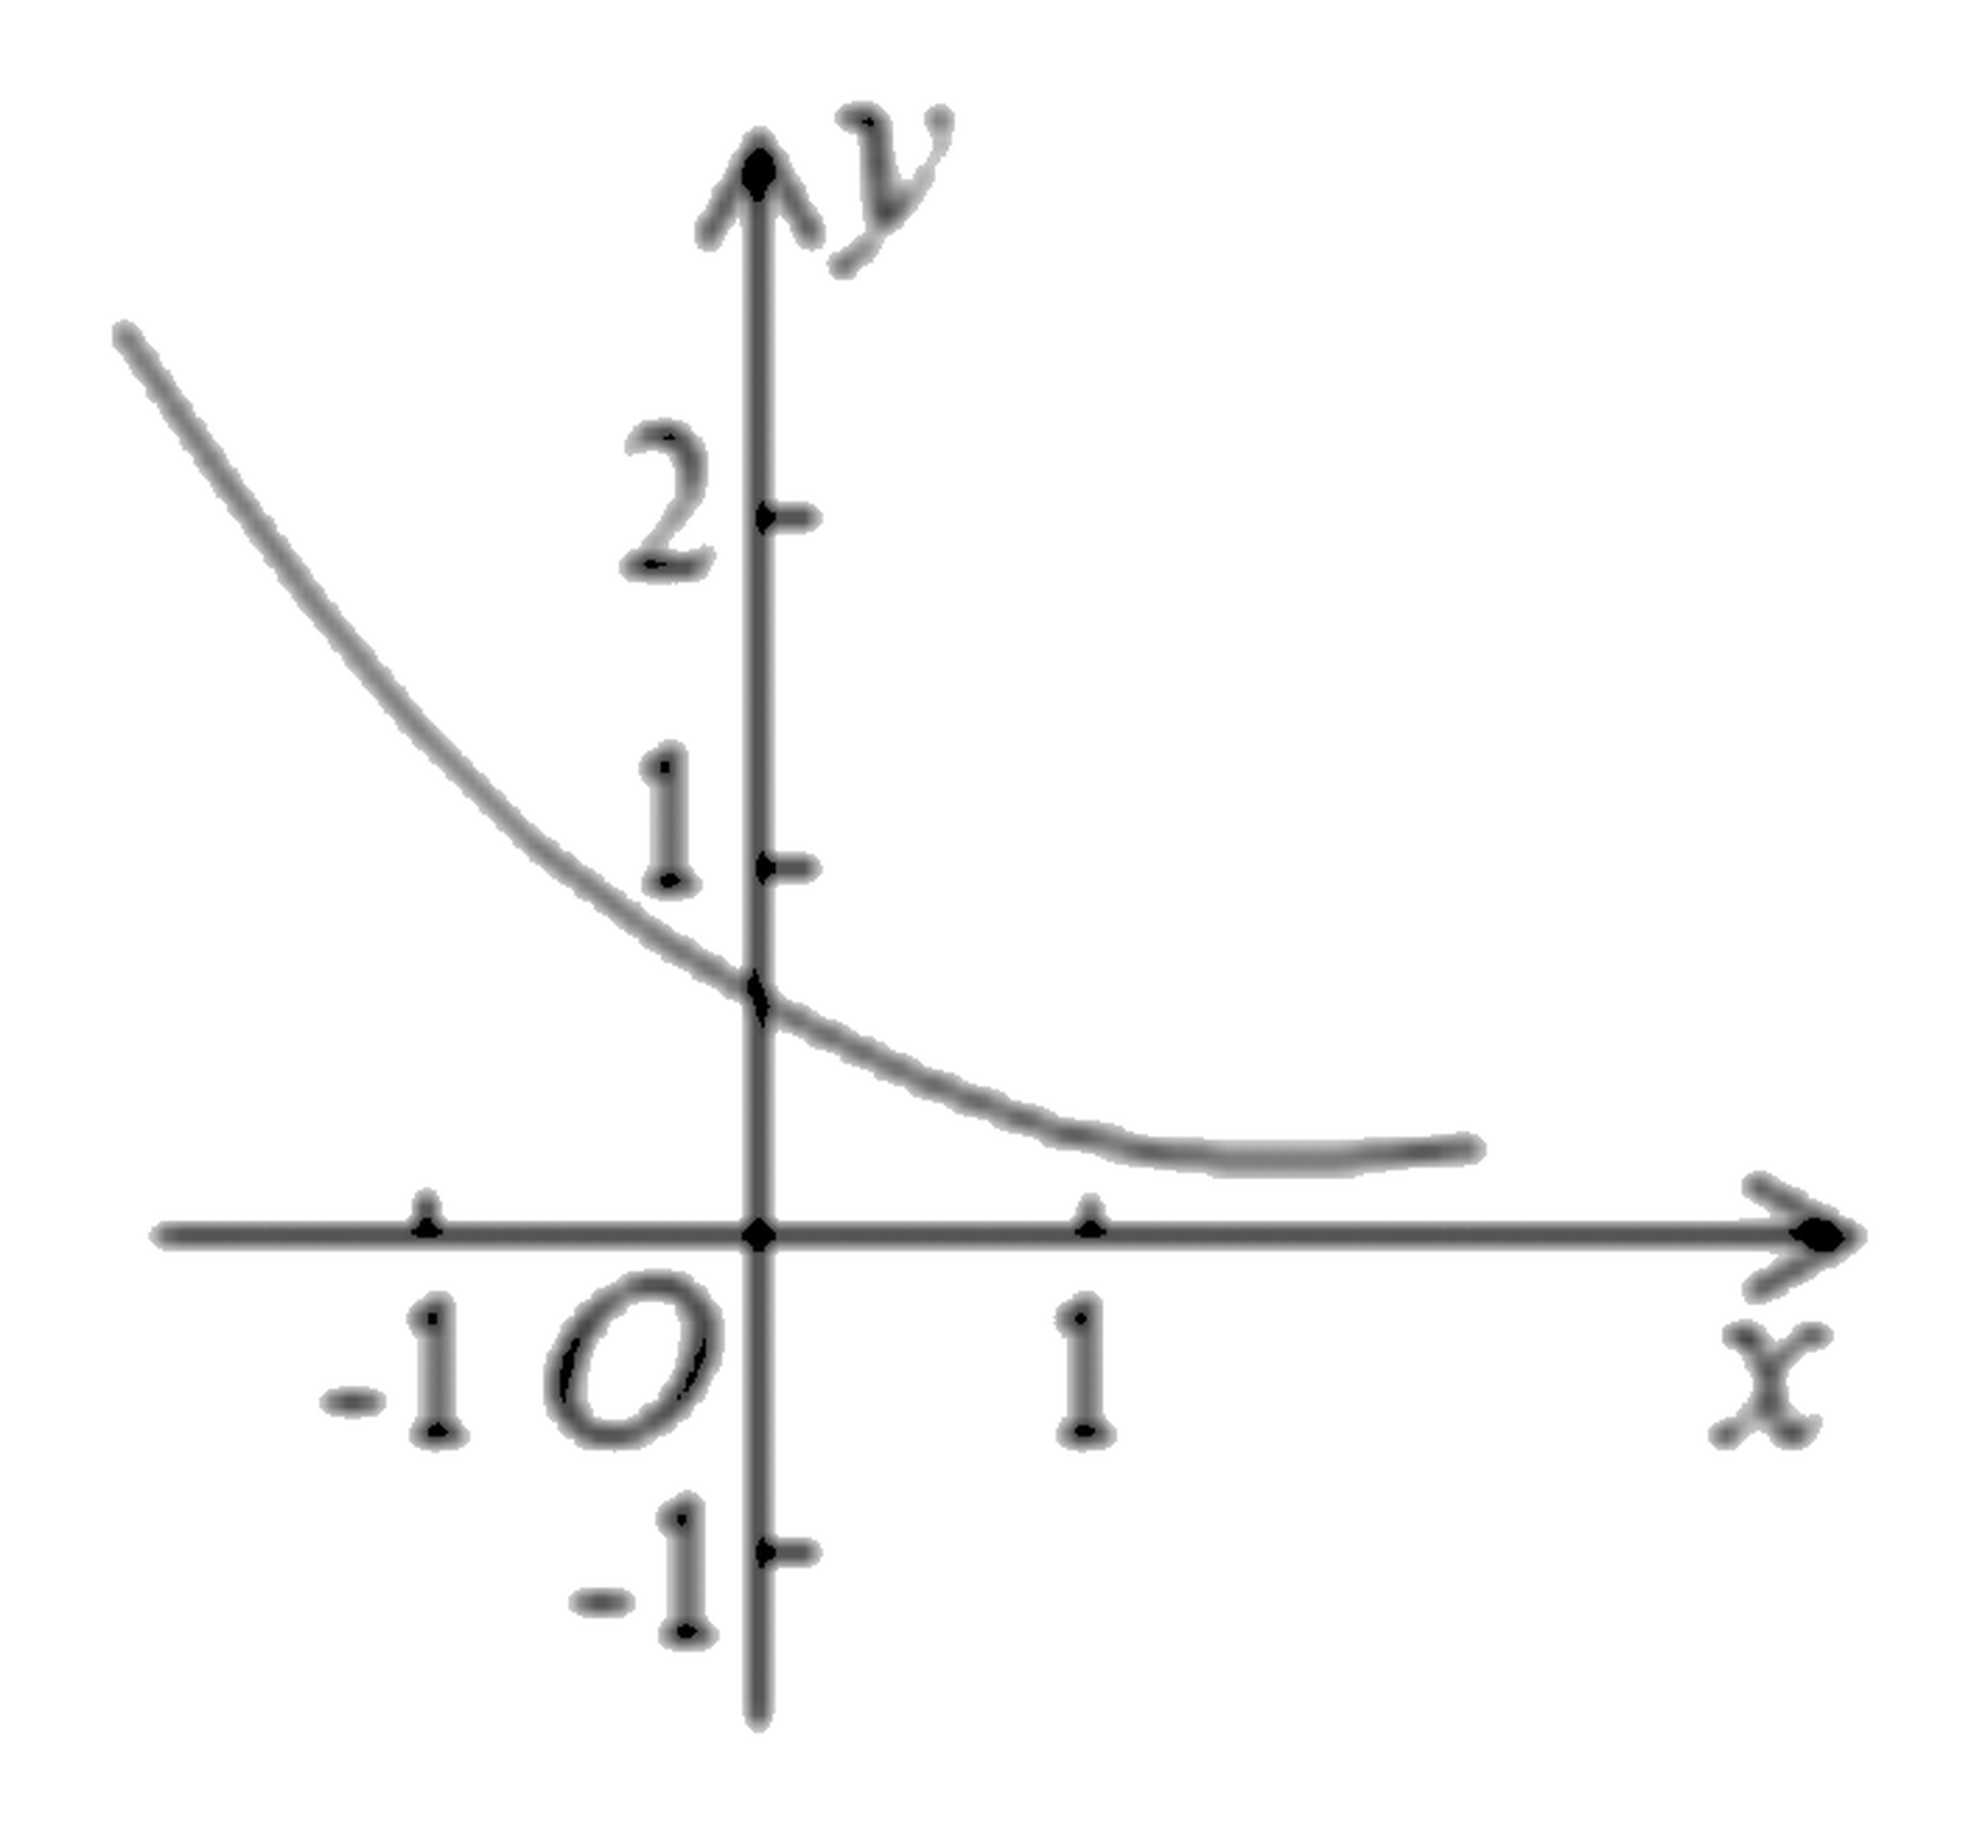
\includegraphics[width=0.30\textwidth]{figures/gao147_q15.png}
\end{center}

\ifanswer
\solbegin
\step{由图象从左到右下降得 $0<a<1$；}
\step{由图象与 $y$ 轴的交点得 $0<a^{-b}<1$，故 $b<0$；}
\step{故 $0<a<1$，$b<0$；故选 $D$.}
\solend
\fi

% === Q16 ===：位数新定义题（无弯引号，放大 04 页 z/q16_stem.png 确认）；四选项横排一行；解析 3 个印刷行
\item 数学运算是指在明晰运算对象的基础上，依据运算法则解决数学问题的素养. 因为运算，数的威力无限；没有运算，数就只是一个符号，对数运算与指数运算是两类重要的运算，对数的运算性质降低了运算的级别，简化了运算，在数学发展史上是伟大的成就. 而位数是指一个自然数有效位的个数，例如：$2^{10}=1024$，所以 $2^{10}$ 的位数为 4. 请你运用所学过的对数运算的知识，估计 $2025^{2026}$ 的位数是\mbox{（\quad）}

\keepwithprev
A. 6697\qquad B. 6698\qquad C. 6699\qquad D. 6700

\ifanswer
\solbegin
\step{设 $2025^{2026}=t$，所以 $\lg t=2026\lg2025$，}
\step{因为 $\lg2025\approx3.3064$，所以 $\lg t\approx6698.8$，}
\step{所以 $t\approx10^{6698.8}\in(10^{6698},10^{6699})$，所以 $2025^{2026}$ 的位数为 6699. 故选 $C$.}
\solend
\fi

\end{enumerate}

\bigsec{三、解答题}

\begin{enumerate}
\setcounter{enumi}{16}

% === Q17 ===：题干＋解析均在 04 页；集合描述竖线 \mid、描述内半角逗号照录；
% 空集 \varnothing、子集 \subseteq（放大 04 页 z/subset_04_q17b.png 确认带下划线）、数集 \R；
% 解析 5 个印刷行，首行末"所以 A=(-∞,-2)∪(3,+∞)"原卷无标点，照录不补
\item 已知集合 $A=\left\{x\mid \dfrac{x+2}{x-3}>0,x\in\R\right\}$，$B=\{x\mid \lvert x-2a\rvert\leqslant2,x\in\R\}$.

(1) 若 $a=1$，求 $A\cap B$；

(2) 若 $A\cap B=\varnothing$，求实数 $a$ 的取值范围.

\ifanswer
\solbegin
\step{由 $\dfrac{x+2}{x-3}>0$，得 $x<-2$ 或 $x>3$，所以 $A=(-\infty,-2)\cup(3,+\infty)$}
\step{(1) 当 $a=1$ 时，$B=\{x\mid \lvert x-2\rvert\leqslant2\}=[0,4]$，于是 $A\cap B=(3,4]$；}
\step{(2) $B=[2a-2,2a+2]$，}
\step{则 $A\cap B=\varnothing\Leftrightarrow[2a-2,2a+2]\subseteq[-2,3]\Leftrightarrow\begin{cases}2a-2\geqslant-2\\2a+2\leqslant3\end{cases}\Leftrightarrow0\leqslant a\leqslant\dfrac{1}{2}$，}
\step{所以实数 $a$ 的取值范围为 $\left[0,\dfrac{1}{2}\right]$.}
\solend
\fi

% === Q18 ===：氟化物／臭氧应用题；"氟化物""（如冰箱等）"全角夹注照录（放大 05 页 z/q18_line1.png 确认）；
% 关系式 $Q=Q_0e^{-0.0025t}$ 原卷独立一行，按一段照录；解析 6 个印刷行
\item 有些家用电器（如冰箱等）使用了氟化物，氟化物的释放破坏了大气上层的臭氧层，使臭氧含量 $Q$ 呈指数函数型变化，在氟化物排放量维持某种水平时，具有关系式

$Q=Q_0e^{-0.0025t}$，其中 $Q_0$ 是臭氧的初始量.

(1) 随时间 $t$ 的增加，臭氧的含量是增加还是减少？

(2) 试估计多少年以后将会有一半的臭氧消失.（用计算器计算）

\ifanswer
\solbegin
\step{(1) 对于函数 $Q=Q_0e^{-0.0025t}$，显然 $Q>0$，}
\step{任取 $t_1$、$t_2\in(0,+\infty)$，且 $t_1<t_2$，则 $t_2-t_1>0$，}
\step{所以 $\dfrac{Q_1}{Q_2}=\dfrac{Q_0e^{-0.0025t_1}}{Q_0e^{-0.0025t_2}}=e^{-0.0025(t_1-t_2)}=e^{0.0025(t_2-t_1)}>e^0=1$，所以 $Q_1>Q_2$，}
\step{故随着时间 $t$ 的增加，臭氧的含量是减少的；}
\step{(2) 令 $\dfrac{Q}{Q_0}=\dfrac{1}{2}$，即 $\dfrac{Q_0e^{-0.0025t}}{Q_0}=e^{-0.0025t}=\dfrac{1}{2}$，得 $-0.0025t=\ln\dfrac{1}{2}\approx-0.6931$，}
\step{解得 $t\approx277$，故估计 277 年以后将会有一半的臭氧消失.}
\solend
\fi

% === Q19 ===：题干用"图像"、解析两处用"图象"逐处照录不统一（05 页）；数集 \Z；
% 题干＋解析前 4 行在 05 页、解析后 3 行在 06 页；解析共 7 个印刷行
\item 已知幂函数 $f(x)=x^{-m^2+4m}(m\in\Z)$ 的图像关于 $y$ 轴对称，且在区间 $(0,+\infty)$ 上是严格增函数.

(1) 求 $m$ 的值；

(2) 求满足不等式 $(2a+1)^m<(a+1)^m$ 的实数 $a$ 的取值范围.

\ifanswer
\solbegin
\step{(1) 由题意得 $-m^2+4m>0$，解得 $0<m<4$，}
\step{因为 $m\in\Z$，所以 $m=1$ 或 $m=2$ 或 $m=3$.}
\step{当 $m=1$ 或 $m=3$ 时，$f(x)=x^3$，图象关于原点对称，不合题意；}
\step{当 $m=2$ 时，$f(x)=x^4$，图象关于 $y$ 轴对称，符合题意，所以 $m=2$.}
\step{(2) 代入 $m=2$，不等式为 $(2a+1)^2<(a+1)^2$，}
\step{得 $(2a+1)^2-(a+1)^2=a(3a+2)<0$，因此 $-\dfrac{2}{3}<a<0$，}
\step{所求范围为 $\left(-\dfrac{2}{3},0\right)$.}
\solend
\fi

% === Q20 ===：指数函数题，题干用"图像"；(3) 长求和式（分数 1/2026、1011/2026、2011/2026、
% 15/2026、1015/2026、2025/2026 放大 06 页 z/q20_sum_06a.png 确认）；题干在 06 页、
% 解析前 6 行在 06 页下半、后 6 行在 07 页上半；解析共 12 个印刷行
\item 已知指数函数 $y=a^x$（$a>0,a\ne1$）的图像经过点 $(1,4)$.

(1) 求实数 $a$ 的值；

(2) 若 $f(x)=(a^x)^2-2\cdot a^x-8$，当 $x\in\R$ 时，不等式 $f(x)>m\cdot4^x-12$ 恒成立，求 $m$ 的取值范围；

(3) 记 $g(x)=\dfrac{1}{a^x+2}$，求证：$g(x)+g(1-x)$ 为定值，并求 $g(0)+g\left(\dfrac{1}{2026}\right)+g\left(\dfrac{1011}{2026}\right)+g\left(\dfrac{2011}{2026}\right)+g\left(\dfrac{1}{2}\right)+g\left(\dfrac{15}{2026}\right)+g\left(\dfrac{1015}{2026}\right)+g\left(\dfrac{2025}{2026}\right)+g(1)$ 的值.

\ifanswer
\solbegin
\step{(1) 将 $(1,4)$ 代入 $y=a^x$，得 $a^1=4$，即 $a=4$.}
\step{(2) 令 $t=4^x$，当 $x\in\R$ 时，$t$ 取遍所有正实数.}
\step{原不等式等价于 $t^2-2t-8>mt-12\Leftrightarrow m<t+\dfrac{4}{t}-2$，}
\step{由基本不等式，$t+\dfrac{4}{t}-2\geqslant2\sqrt{t\cdot\dfrac{4}{t}}-2=2$，}
\step{当且仅当 $t=\dfrac{4}{t}$，即 $t=2$ 时取等号，}
\step{因此原不等式恒成立的充要条件为 $m<2$，即 $m\in(-\infty,2)$.}
\step{(3) 对任意 $x\in\R$，令 $t=4^x>0$，则 $4^{1-x}=\dfrac{4}{t}$，}
\step{从而 $g(x)+g(1-x)=\dfrac{1}{t+2}+\dfrac{1}{\dfrac{4}{t}+2}=\dfrac{1}{t+2}+\dfrac{t}{2(t+2)}=\dfrac{1}{2}$，}
\step{因此 $g(x)+g(1-x)$ 为定值 $\dfrac{1}{2}$.}
\step{原式中，0 与 1、$\dfrac{1}{2026}$ 与 $\dfrac{2025}{2026}$、$\dfrac{1011}{2026}$ 与 $\dfrac{1015}{2026}$、$\dfrac{2011}{2026}$ 与 $\dfrac{15}{2026}$}
\step{分别配对，每对函数值之和均为 $\dfrac{1}{2}$，且 $g\left(\dfrac{1}{2}\right)=\dfrac{1}{4^{\frac12}+2}=\dfrac{1}{4}$，}
\step{所以所求和为 $4\cdot\dfrac{1}{2}+\dfrac{1}{4}=\dfrac{9}{4}$.}
\solend
\fi

% === Q21 ===：不动点新定义题；题干在 07 页、解析续 08／09 页，共 20 个印刷行；
% 判别式两形混用：08 页 (2) cases 内等腰偏高 \Delta、09 页 (3) 扁等边 \triangle，逐处照录不统一
% （放大 /tmp/gao147/z/delta_vs_triangle.png 并排确认）；数集 \R；\forall 照录；
% 第 6—8 行是原卷一个长算式折成的三个印刷行，按印刷行分三条 \step、不并折行
\item 对于二次函数 $y=mx^2+nx+t(m\ne0)$，若存在 $x_0\in\R$，使得 $mx_0^2+nx_0+t=x_0$ 成立，则称 $x_0$ 为二次函数 $y=mx^2+nx+t(m\ne0)$ 的不动点.

(1) 求二次函数 $y=x^2-x-3$ 的不动点；

(2) 若二次函数 $y=2x^2-(3+a)x+a-1$ 有两个不相等的不动点 $x_1$、$x_2$，且 $x_1$、$x_2>0$，求 $\dfrac{x_1}{x_2}+\dfrac{x_2}{x_1}$ 的最小值；

(3) 若对任意实数 $b$，二次函数 $y=ax^2+(b+1)x+(b-1)(a\ne0)$ 恒有不动点，求 $a$ 的取值范围.

\ifanswer
\solbegin
\step{(1) 令 $x^2-x-3=x$，即 $x^2-2x-3=0$，即 $(x-3)(x+1)=0$，}
\step{解得 $x_1=-1$，$x_2=3$，所以不动点为 $-1$ 和 $3$.}
\step{(2) 由题意，$2x^2-(3+a)x+a-1=x$ 有两个不相等的正实数根，}
\step{即方程 $2x^2-(4+a)x+a-1=0$ 有两个不相等的正实数根，}
\step{所以 $\begin{cases}\Delta=(4+a)^2-8(a-1)>0\\x_1+x_2=\dfrac{4+a}{2}>0\\x_1\cdot x_2=\dfrac{a-1}{2}>0\end{cases}$，解得 $a>1$，}% 判别式原卷印等腰偏高粗三角 $\Delta$（放大 08 页 z/delta_08_q21cases.png）
\step{所以 $\dfrac{x_1}{x_2}+\dfrac{x_2}{x_1}=\dfrac{x_1^2+x_2^2}{x_1\cdot x_2}=\dfrac{(x_1+x_2)^2-2x_1\cdot x_2}{x_1\cdot x_2}=\dfrac{(x_1+x_2)^2}{x_1\cdot x_2}-2$}
\step{$=\dfrac{\left(\dfrac{4+a}{2}\right)^2}{\dfrac{a-1}{2}}-2=\dfrac{\dfrac{(a+4)^2}{4}}{\dfrac{a-1}{2}}-2=\dfrac{(a-1+5)^2}{2(a-1)}-2$}
\step{$=\dfrac{(a-1)^2+10(a-1)+25}{2(a-1)}-2=\dfrac{a-1}{2}+\dfrac{25}{2(a-1)}+3$.}
\step{因为 $a>1$，所以 $a-1>0$，}
\step{所以 $\dfrac{a-1}{2}+\dfrac{25}{2(a-1)}+3\geqslant2\sqrt{\dfrac{a-1}{2}\cdot\dfrac{25}{2(a-1)}}+3=8$，}
\step{当且仅当 $\dfrac{a-1}{2}=\dfrac{25}{2(a-1)}$，即 $a=6$ 时等号成立，}
\step{所以 $\dfrac{x_1}{x_2}+\dfrac{x_2}{x_1}$ 的最小值为 $8$.}
\step{(3) 设 $f(x)=ax^2+(b+1)x+b-1$，}
\step{则方程 $f(x)=x$，可化为 $ax^2+(b+1)x+b-1=x$，}
\step{即 $ax^2+bx+b-1=0$，}
\step{由题意得一元二次方程 $ax^2+bx+b-1=0$ 有解，又 $a\ne0$，}
\step{所以方程 $ax^2+bx+b-1=0$ 的判别式 $\triangle=b^2-4a(b-1)\geqslant0$，}% 判别式原卷印扁等边细线三角 $\triangle$（放大 09 页 z/triangle_09_q21.png），与 (2) 高 $\Delta$ 混用、照录不统一
\step{即 $b^2-4ab+4a\geqslant0$，则该不等式对 $\forall b\in\R$ 恒成立，}
\step{则 $(4a)^2-4\times4a\leqslant0$，且 $a\ne0$，解得 $0<a\leqslant1$，}
\step{所以实数 $a$ 的取值范围是 $(0,1]$.}
\solend
\fi

\end{enumerate}

\end{document}
"
% 紧凑版：xelatex "\def\iscompact{1}% 高一147_华师大三附中_期中.tex
%   —— 高一上数学"2026-2027 年华师大三附中高一上期中"（试卷版/答案版/紧凑版）
% 试卷版：xelatex 高一147_华师大三附中_期中.tex
% 答案版：xelatex "\def\isanswer{1}\input{高一147_华师大三附中_期中.tex}"
% 紧凑版：xelatex "\def\iscompact{1}\input{高一147_华师大三附中_期中.tex}"
%
% ① 原始材料：微信公众号"魔都数学加油站"文章，连载"27学年高一147"，原文标题
% "27学年高一147——2026-2027年上海市华师大三附中高一上期中"；
% 原文链接：https://mp.weixin.qq.com/s/X_gPW1JWoTAl2Bky_xEEGw 。
% 正文为 9 张 PNG 页（01/06/08/09 为 2560×3620，02/03/04/05/07 为 4762×6735，
% 同一篇各页分辨率混排，逐页按各自分辨率裁图核对，别按预览比例换算裁框）。
% 体例：混合体例讲评版——19 题中 Q4/Q5/Q7/Q9 只印【答案】、无【解析】，其余 15 题印
% 【解析】（逐题核实，见 ② ②）。题目、答案、解析均据原图转录；卷面粉红色水印
% "魔都数学加油站"及公众号页脚未录入。
% 全卷插图清单（逐页通读 9 页确认）：仅 1 处题目配图——
%   · Q15 递减指数函数小坐标系（03 页右侧：坐标轴、y 轴刻度 2/1/-1、x 轴刻度 -1/1、
%     原点 O、x/y 轴标），为"图像如图所示"的题目配图（选择题选项旁），三版都出；
%     裁自 03 页去粉色水印、去色、4× LANCZOS 放大存 figures/gao147_q15.png；
%   其余 8 页逐页确认无其它题目配图、无【解析】内配图、无表格，
%   亦无"题干写如图而源码漏图"一处；Q12/Q17/Q21 的 cases 块为数学块（非图）。
%
% 卷首标题：原卷印作"2026-2027 年华师大三附中高一上期中"，年份区间按全稿惯例排 en dash；
% 原卷卷面未印副标题，本稿按同期中卷（高一140／141／143／144／145／146）知识模块口径
% 补出"集合与常用逻辑用语、不等式、函数"。
%
% 题号体例（逐页核实定稿）：本卷共 19 题——一、填空题 3—12（10 题）、
% 二、选择题 13—16（4 题）、三、解答题 17—21（5 题）。
% 三节分别 \setcounter{enumi}{2}／{12}／{16}。原卷从第 3 题起、无第 1、2 题，
% 本稿保留原题号；全卷无附加题节（Q21 解析末行"所以实数 a 的取值范围是 (0,1]."
% 为全卷收尾，09 页下半仅水印、无正文）。
%
% ② 与原卷的排版差异：
%   ① 原文从第 3 题起，本稿保留原题号；共 19 题三节；
%   ② 混合体例：原卷 Q4/Q5/Q7/Q9 只印【答案】、无【解析】（分别为 a≤0、(-1,2)、
%      真、(-∞,1)），按 高一140 第 5 题／高一145 Q3 成例提 \ans{}、不补造解析；
%      其余 15 题印【解析】，用 \solbegin…\solend，选择题答案在解析末句"故选 X"
%      （Q13 选 B、Q14 选 B、Q15 选 D、Q16 选 C，逐个放大原图核实）、题干括号
%      \mbox{（\quad）} 留空、不另提 \ans{}；填空／解答答案落在解析里；
%      答案版【答案】/【解析】标记数 = 19（4 个 \ans ＋ 15 个 \solbegin）= 全卷题数；
%   ③ 原卷卷面未印副标题，本稿按知识模块口径补出；
%   ④ 原卷填空横线按全稿惯例排 \blankline[4.4em]；选择题括号排 \mbox{（\quad）}、
%      选项段前按惯例加 \keepwithprev；Q14／Q15 四选项为 2×2 两印刷行（A/B 一行、
%      C/D 一行），用空行分段照录（非一行 \qquad、亦非竖排四行）；解答题不留作答区、
%      不加 \anspace（原卷为讲评版，与 129／131／132／133／136／140／141／143／144／145／146 同）；
%   ⑤ 数集：Q4"A∪B=R"、Q13"f(x)=x^3 在 R 上严格增"、Q17"x∈R"两处、
%      Q20"x∈R"两处、Q21"x_0∈R""∀b∈R"原卷印斜体或黑板粗体 R，按全稿惯例统一改 \R；
%      Q19"m∈Z"改 \Z；本卷未出现 N（\N^* 无对应处）。绝对值排 \lvert…\rvert，
%      集合描述竖线排 \mid；不等号按全稿惯例排 \leqslant／\geqslant（原卷印 \le／\ge 形，
%      【答案】a≤0 亦排 \leqslant）；空集 \varnothing（Q17 两处）；
%      子集 \subseteq（Q17 带下划线，放大 04 页确认）；本卷未出现 \subset／\subsetneq，
%      亦未出现补集上划线 \overline{}；\left…\right 不得拆到不同 $…$ 组；
%   ⑥ 子题标号 (1)(2)(3) 半角括号照录；cases 块整体算一个印刷行（Q3、Q12 一行内
%      两个 cases、Q17、Q21(2)）；本卷解析内无圈数字①②③（无 \text{①} 需求）；
%      数学式内 CJK 用 \text{}（本卷未见）；
%   ⑦ 题干中的中文弯引号按原卷照录：Q7 命题"若 A∪B=B，则 A∩B=A"与
%      (填 " 真 " 或 " 假 ")、Q10 (填 ">" "<" "≤" "或≥")，含引号内空格；
%      注释内一律 ASCII 引号；Q16 位数新定义题逐字放大确认无弯引号
%      （交办提示的"Q16 新定义题"举例未在本卷出现），未补造引号；
%   ⑧ 半角逗号在数学组之间是全稿惯例、非笔误（Q4"$A=(-\infty,0],B=[a,+\infty)$"、
%      Q5"$(a>0,a\ne1)$"、Q17 集合描述内"$>0,x\in R$""$\leqslant2,x\in R$"、
%      Q20 题干"$(a>0,a\ne1)$"、Q21"$y=mx^2+nx+t(m\ne0)$"等），逐处照录别改全角；
%      行末西文句点照录为 ASCII `.`；行中全角逗号／顿号照录；
%      Q7／Q10"(填…)"为半角括号、Q18"（如冰箱等）"为全角括号，逐处照录不统一；
%   ⑨ "图像／图象"逐处照录不统一：题干 5 处用"图像"（Q5"图像恒过定点"、
%      Q9"图像位于直线 y=x 的下方"、Q15"的图像如图所示"、Q19"的图像关于 y 轴对称"、
%      Q20"的图像经过点"），解析 4 处用"图象"（Q15"由图象从左到右下降"
%      "由图象与 y 轴的交点"、Q19"图象关于原点对称""图象关于 y 轴对称"），逐处核、不统一；
%   ⑩ 判别式 Δ/△ 混用是照录项：Q21(2) 解析 cases 块"Δ=(4+a)²−8(a−1)>0"
%      印等腰偏高粗三角 \Delta，Q21(3) 解析"判别式△=b²−4a(b−1)≥0"
%      印扁等边细线三角 \triangle，逐处放大判断、照录不得统一
%      （参照 高一142／144／145 头注④口径，详见 ④）；
%   ⑪ 一条 \step = 原卷解析的一个印刷行，cases 块整体算一个印刷行；别把原卷折行
%      并起来、别把一行拆多条。Q10 七行（跨 01→02 页）、Q12 七行（含一行两 cases）、
%      Q20 十二行（含"原式中…2011/2026 与 15/2026／分别配对…"折行两行）、
%      Q21 二十行（含第 6—8 行一个长算式折成三印刷行、含 cases）均按印刷行逐条断，
%      不丢行；
%   ⑫ 配图：逐页通读 9 页确认全卷仅 Q15 一处题目配图（见 ①），三版都出、
%      \includegraphics[width=0.30\textwidth]；图块较小，未加 \needvspace 大图块守卫
%      （仅 \bigsec 自带 \needvspace{3\baselineskip}）；三版切页审计均"合计异常：无"；
%   ⑬ 跨页续印按题合并：Q3—Q9 在 01 页（Q10 题干在 01 页末、解析首行亦在 01 页末）；
%      Q10 解析续 02 页 6 行、Q11 在 02 页、Q12 题干＋解析前 4 行在 02 页
%      （解析续 03 页 3 行）；"二、选择题"标题与 Q13、Q14、Q15 题干＋解析前 2 行在 03 页
%      （Q15 配图在 03 页右侧）；Q15 解析末行与 Q16、"三、解答题"标题、Q17 在 04 页；
%      Q18 在 05 页、Q19 题干＋解析前 4 行在 05 页（解析续 06 页 3 行）；
%      Q20 题干＋解析前 6 行在 06 页（解析续 07 页 6 行）、Q21 题干＋解析前 3 行在 07 页；
%      Q21 解析续 08 页 13 行、续 09 页 4 行（09 页下半仅水印、无正文）。
%      本稿按题连排，不丢行、不并折行；
%   ⑭ 原卷解析内无红色"法一／法二"之类小标题，故本卷无 \stepm；
%      水印"魔都数学加油站"红色不录入。
%
% ③ 行数复核：一条 \step／\stepm = 原卷解析的一个印刷行，cases 块作一个印刷行计。
%   逐题数（主会话逐页核对定稿）：Q3：1；Q4：0（只印【答案】、提 \ans{}，不计入 \step 账）；
%   Q5：0；Q6：1；Q7：0；Q8：2；Q9：0；Q10：7；Q11：4；Q12：7；Q13：6；Q14：4；
%   Q15：3；Q16：3；Q17：5；Q18：6；Q19：7；Q20：12；Q21：20。
%   合计 88 条 \step（本卷无 \stepm：解析内无红色"法一／法二"类小标题），
%   与原卷逐题印刷行相等。全卷 15 题设 \solbegin…\solend ＋ 4 题一处 \ans{}，
%   答案版【答案】/【解析】标记数 = 19 = 全卷题数。
%
% ④ 判别式／子集符号结论（逐处放大原图照录、不得统一，主会话像素级复核）：
%   判别式全卷 2 处、两形混用逐处照录不统一（参照 高一142／144 头注④口径）：
%     · Q21(2) 解析 cases 块"Δ=(4+a)²−8(a−1)>0" 原卷印等腰偏高粗三角
%       （高>宽、粗笔画），照录 \Delta（放大 08 页 /tmp/gao147/z/delta_08_q21cases.png
%       与 z/delta_vs_triangle.png 左图确认）；
%     · Q21(3) 解析"判别式△=b²−4a(b−1)≥0" 原卷印扁等边细线三角
%       （宽≈高、细线），照录 \triangle（放大 09 页 /tmp/gao147/z/triangle_09_q21.png
%       与 z/delta_vs_triangle.png 右图并排确认）。
%   子集／补集：Q17 解析"[2a−2,2a+2]⊆[−2,3]" 原卷印带下划线 ⊆，照录 \subseteq
%     （放大 04 页 /tmp/gao147/z/subset_04_q17b.png 确认）；Q17"A∩B=∅"空集 \varnothing；
%     集合描述竖线 \mid（Q10 M、Q12 解集、Q17 A/B）；并集 \cup（Q4、Q17）、
%     交集 \cap（Q7、Q17）、不属于 \notin（Q10）；数集 \R／\Z 归一见 ② ⑤。
%   本卷未出现 \subset／\subsetneq，未出现补集上划线 \overline{}。
%
% ⑤ 存疑照录（放大原图确认，照录未改、正文对应处另有 % 注）：
%   1. Q4/Q5/Q7/Q9 只印【答案】、无【解析】，按成例提 \ans{}、不补造解析
%      （混合体例逐题核实，见 ② ②）。
%   2. Q21(2) 判别式高 \Delta 与 Q21(3) 判别式扁 \triangle 两形混用，
%      逐处照录不统一（见 ④）。
%   3. "图像／图象"题干 5 处"图像"、解析 4 处"图象"，逐处照录不统一（见 ② ⑨）。
%   4. Q7／Q10"(填…)"半角括号与 Q18"（如冰箱等）"全角括号，逐处照录不统一。
%   5. Q16 位数新定义题逐字放大确认无弯引号（交办提示的"Q16 新定义题"举例
%      未在本卷出现），未补造引号；全卷弯引号仅 Q7、Q10 两处。
%   6. Q17 解析首行末"所以 A=(-∞,-2)∪(3,+∞)"、Q20(3) 解析"…2011/2026 与 15/2026"
%      行末原卷均无标点，照录未补；Q21(2) 第 6—8 行一个长算式折成三印刷行，
%      按印刷行分三条 \step、不并折行。
%   全卷除此 6 类外未发现其它笔误／自相矛盾处。
%
% ⑥ 跨页续印按题合并说明：见 ② ⑬。
%
\documentclass[a4paper,11pt]{article}
\usepackage{common}

\begin{document}

\examtitlest[3]{2026--2027 年华师大三附中高一上期中}{集合与常用逻辑用语、不等式、函数}

\bigsec{一、填空题}

\begin{enumerate}
\setcounter{enumi}{2}

% === Q3 ===：印【解析】，1 个印刷行（cases 块整体算一行）
\item 函数 $y=(a^2-5a+7)a^x+6-2a$ 是指数函数，则 $a$ 的值为\blankline[4.4em].

\ifanswer
\solbegin
\step{由题意得 $\begin{cases}a^2-5a+7=1\\6-2a=0\end{cases}$，解得 $a=3$.}
\solend
\fi

% === Q4 ===：原卷只印【答案】、无【解析】，按 高一140 第 5 题／高一145 Q3 成例提 \ans{}、不补造解析；
% 题干数学组内半角逗号 $A=(-\infty,0],B=[a,+\infty)$ 照录（放大 01 页 z/q4_stem.png 确认）
\item 已知 $A=(-\infty,0],B=[a,+\infty)$，且 $A\cup B=\R$，则实数 $a$ 的取值范围为\blankline[4.4em].

\ifanswer
\ans{$a\leqslant0$}
\fi

% === Q5 ===：只印【答案】；题干"图像"照录（放大 01 页 z/q5_stem.png 确认）；
% 数学组内半角逗号 $(a>0,a\ne1)$ 照录
\item 函数 $y=a^{x+1}+1(a>0,a\ne1)$ 的图像恒过定点\blankline[4.4em].

\ifanswer
\ans{$(-1,2)$}
\fi

% === Q6 ===：印【解析】，1 个印刷行
\item 已知方程 $x^2+2x-4=0$ 的两个根为 $x_1$、$x_2$，则 $x_1^2+x_2^2$ 的值为\blankline[4.4em].

\ifanswer
\solbegin
\step{$x_1^2+x_2^2=(x_1+x_2)^2-2x_1x_2=4+8=12$.}
\solend
\fi

% === Q7 ===：只印【答案】；中文弯引号"若 A∪B=B，则 A∩B=A"与(填 " 真 " 或 " 假 ")内的空格照录
% （放大 01 页 z/q7_quotes_7x.png、z/q7_tail.png 确认，括号为半角）
\item 命题 “若 $A\cup B=B$，则 $A\cap B=A$” 为\blankline[4.4em]命题(填 “ 真 ” 或 “ 假 ”).

\ifanswer
\ans{真}
\fi

% === Q8 ===：印【解析】，2 个印刷行；不等号按全稿惯例 \geqslant／\leqslant
\item 已知正实数 $a$、$b$ 满足 $a+4b=1$，则 $ab$ 的最大值为\blankline[4.4em].

\ifanswer
\solbegin
\step{$a+4b\geqslant2\sqrt{a\cdot4b}\Rightarrow ab\leqslant\dfrac{1}{16}$，当且仅当 $a=4b=\dfrac{1}{2}$ 时取等号，}
\step{则 $ab$ 的最大值为 $\dfrac{1}{16}$.}
\solend
\fi

% === Q9 ===：只印【答案】；题干"图像"照录（放大 01 页 hi_01_2 确认）
\item 若幂函数 $y=x^s$ 在 $x>1$ 时的图像位于直线 $y=x$ 的下方，则 $s$ 的取值范围是\blankline[4.4em].

\ifanswer
\ans{$(-\infty,1)$}
\fi

% === Q10 ===：印【解析】，共 7 个印刷行（题在 01 页末起 1 行、续 02 页 6 行）；
% 题干跨两印刷行"则 |ab|+1 ____ |a|+|b|（填…）"按一句连排；(填…)为半角括号、引号内空格照录
\item 已知不等式 $\lvert2x+1\rvert+\lvert2x-1\rvert<4$ 的解集为 $M$. 设实数 $a\in M$，$b\notin M$，则 $\lvert ab\rvert+1$\blankline[4.4em] $\lvert a\rvert+\lvert b\rvert$(填 “$>$”，“$<$”，“$\leqslant$” “或$\geqslant$”).

\ifanswer
\solbegin
\step{当 $x<-\dfrac{1}{2}$ 时，不等式化为 $-2x-1+1-2x<4$，即 $x>-1$，所以 $-1<x<-\dfrac{1}{2}$；}
\step{当 $-\dfrac{1}{2}\leqslant x\leqslant\dfrac{1}{2}$ 时，不等式化为 $2x+1-2x+1<4$，即 $2<4$，所以 $-\dfrac{1}{2}\leqslant x\leqslant\dfrac{1}{2}$；}
\step{当 $x>\dfrac{1}{2}$ 时，不等式化为 $2x+1+2x-1<4$，即 $x<1$，所以 $\dfrac{1}{2}<x<1$；}
\step{综上，$M=\{x\mid -1<x<1\}$.}
\step{因为 $a\in M$，$b\notin M$，所以 $\lvert a\rvert<1$，$\lvert b\rvert\geqslant1$.}
\step{而 $\lvert ab\rvert+1-(\lvert a\rvert+\lvert b\rvert)=\lvert ab\rvert+1-\lvert a\rvert-\lvert b\rvert=(\lvert a\rvert-1)(\lvert b\rvert-1)$，}
\step{所以 $\lvert ab\rvert+1\leqslant\lvert a\rvert+\lvert b\rvert$.}
\solend
\fi

% === Q11 ===：印【解析】，4 个印刷行（02 页）
\item 已知 $m>1$，$n>1$，$\lg m=\log_n100$，则 $mn$ 的最小值为\blankline[4.4em].

\ifanswer
\solbegin
\step{由 $m>1$，$n>1$，得 $\lg m>0$，$\lg n>0$，}
\step{因为 $\lg m=\log_n100=\dfrac{\lg100}{\lg n}=\dfrac{2}{\lg n}$，所以 $\lg m\cdot\lg n=2$，}
\step{所以 $\lg(mn)=\lg m+\lg n\geqslant2\sqrt{\lg m\cdot\lg n}=2\sqrt2$，}
\step{当且仅当 $m=n=10^{\sqrt2}$ 时取等号，则 $mn\geqslant10^{2\sqrt2}$，即 $mn$ 的最小值为 $10^{2\sqrt2}$.}
\solend
\fi

% === Q12 ===：印【解析】，共 7 个印刷行（02 页 4 行、03 页 3 行）；
% 第 3 行"则 [cases]，得 [cases]，"两个 cases 块同属一个印刷行，整体作一条 \step（照 高一146 Q11 成例）
\item 已知关于 $x$ 的不等式 $ax^2+bx+c\leqslant1$ 的解集为 $\{x\mid -1\leqslant x\leqslant3\}$. 若关于 $x$ 的不等式 $ax^2+(b-1)x+c-2\leqslant0$ 有且仅有 8 个整数解，则实数 $a$ 的取值范围是\blankline[4.4em].

\ifanswer
\solbegin
\step{由已知关于 $x$ 的不等式 $ax^2+bx+c\leqslant1$ 的解集为 $\{x\mid -1\leqslant x\leqslant3\}$，}
\step{得 $a>0$，且方程 $ax^2+bx+c-1=0$ 的两根分别为 $-1$ 和 $3$，}
\step{则 $\begin{cases}-1+3=-\dfrac{b}{a}\\-1\times3=\dfrac{c-1}{a}\end{cases}$，得 $\begin{cases}b=-2a\\c=1-3a\end{cases}$，}
\step{不等式 $ax^2+(b-1)x+c-2\leqslant0$ 等价于 $ax^2-(2a+1)x-(3a+1)\leqslant0$，}
\step{即 $\left[x-\left(3+\dfrac{1}{a}\right)\right](x+1)\leqslant0$，解得 $-1\leqslant x\leqslant3+\dfrac{1}{a}$，}
\step{因为关于 $x$ 的不等式 $ax^2+(b-1)x+c-2\leqslant0$ 有且仅有 8 个整数解，}
\step{因此 $6\leqslant3+\dfrac{1}{a}<7$，即 $3\leqslant\dfrac{1}{a}<4$，解得 $\dfrac{1}{4}<a\leqslant\dfrac{1}{3}$，所以 $a$ 的取值范围为 $\left(\dfrac{1}{4},\dfrac{1}{3}\right]$.}
\solend
\fi

\end{enumerate}

\bigsec{二、选择题}

\begin{enumerate}
\setcounter{enumi}{12}

% === Q13 ===：题干＋选项＋解析均在 03 页；四选项横排一行；解析 6 个印刷行，末句"故选 B."
\item $a<b<0$，则下列不等式能成立的是\mbox{（\quad）}

\keepwithprev
A. $\dfrac{a}{b}<1$\qquad B. $\lvert a\rvert>-b$\qquad C. $\dfrac{1}{a}<\dfrac{1}{b}$\qquad D. $b^3<a^3$

\ifanswer
\solbegin
\step{对于 $A$，令 $a=-4$，$b=-3$，满足 $a<b<0$，但 $\dfrac{a}{b}>1$，故 $A$ 错误，}
\step{对于 $B$，因为 $a<b<0$，所以 $-a>-b>0$，即 $\lvert a\rvert>-b$，故 $B$ 正确，}
\step{对于 $C$，令 $a=-4$，$b=-3$，满足 $a<b<0$，但 $\dfrac{1}{a}>\dfrac{1}{b}$，故 $C$ 错误，}
\step{对于 $D$，$f(x)=x^3$ 在 $\R$ 上严格增，因为 $a<b$，所以 $f(a)<f(b)$，}
\step{即 $a^3<b^3$，故 $D$ 错误.}
\step{故选 $B$.}
\solend
\fi

% === Q14 ===：四选项原卷为 2×2 两印刷行（A/B 一行、C/D 一行），用空行分段照录；解析 4 个印刷行
\item 已知 $a$、$b$ 为实数，若 $\alpha:ab=0$，$\beta:a^2+\sqrt{b}=0$，则 $\alpha$ 是 $\beta$ 的\mbox{（\quad）}

\keepwithprev
A. 充分不必要条件\qquad\qquad B. 必要不充分条件

C. 充要条件\qquad\qquad D. 既不充分也不必要条件

\ifanswer
\solbegin
\step{$\beta:a^2+\sqrt{b}=0$，所以 $a=0$ 且 $b=0$，}
\step{由 $a=0$，$b=0\Rightarrow ab=0$，反之不成立.}
\step{所以 $ab=0$ 是 $a=0$，$b=0$ 的必要不充分条件，即 $\alpha$ 是 $\beta$ 的必要不充分条件，}
\step{故选 $B$.}
\solend
\fi

% === Q15 ===：题目配图（03 页右侧小坐标系），三版都出；题干用"图像"、解析用"图象"逐处照录；
% 四选项 2×2 两印刷行；解析 3 个印刷行（03 页 2 行、04 页 1 行，末句"故选 D."与前行同一印刷行）
\item 函数 $f(x)=a^{x-b}$ 的图像如图所示，其中 $a$、$b$ 为常数，则下列结论正确的是\mbox{（\quad）}

\keepwithprev
A. $a>1$，$b<0$\qquad\qquad B. $a>1$，$b>0$

C. $0<a<1$，$b>0$\qquad\qquad D. $0<a<1$，$b<0$

\begin{center}
% 递减指数函数小坐标系图取 03 页右侧，去粉色水印、去色、4× LANCZOS 放大；题目配图三版都出
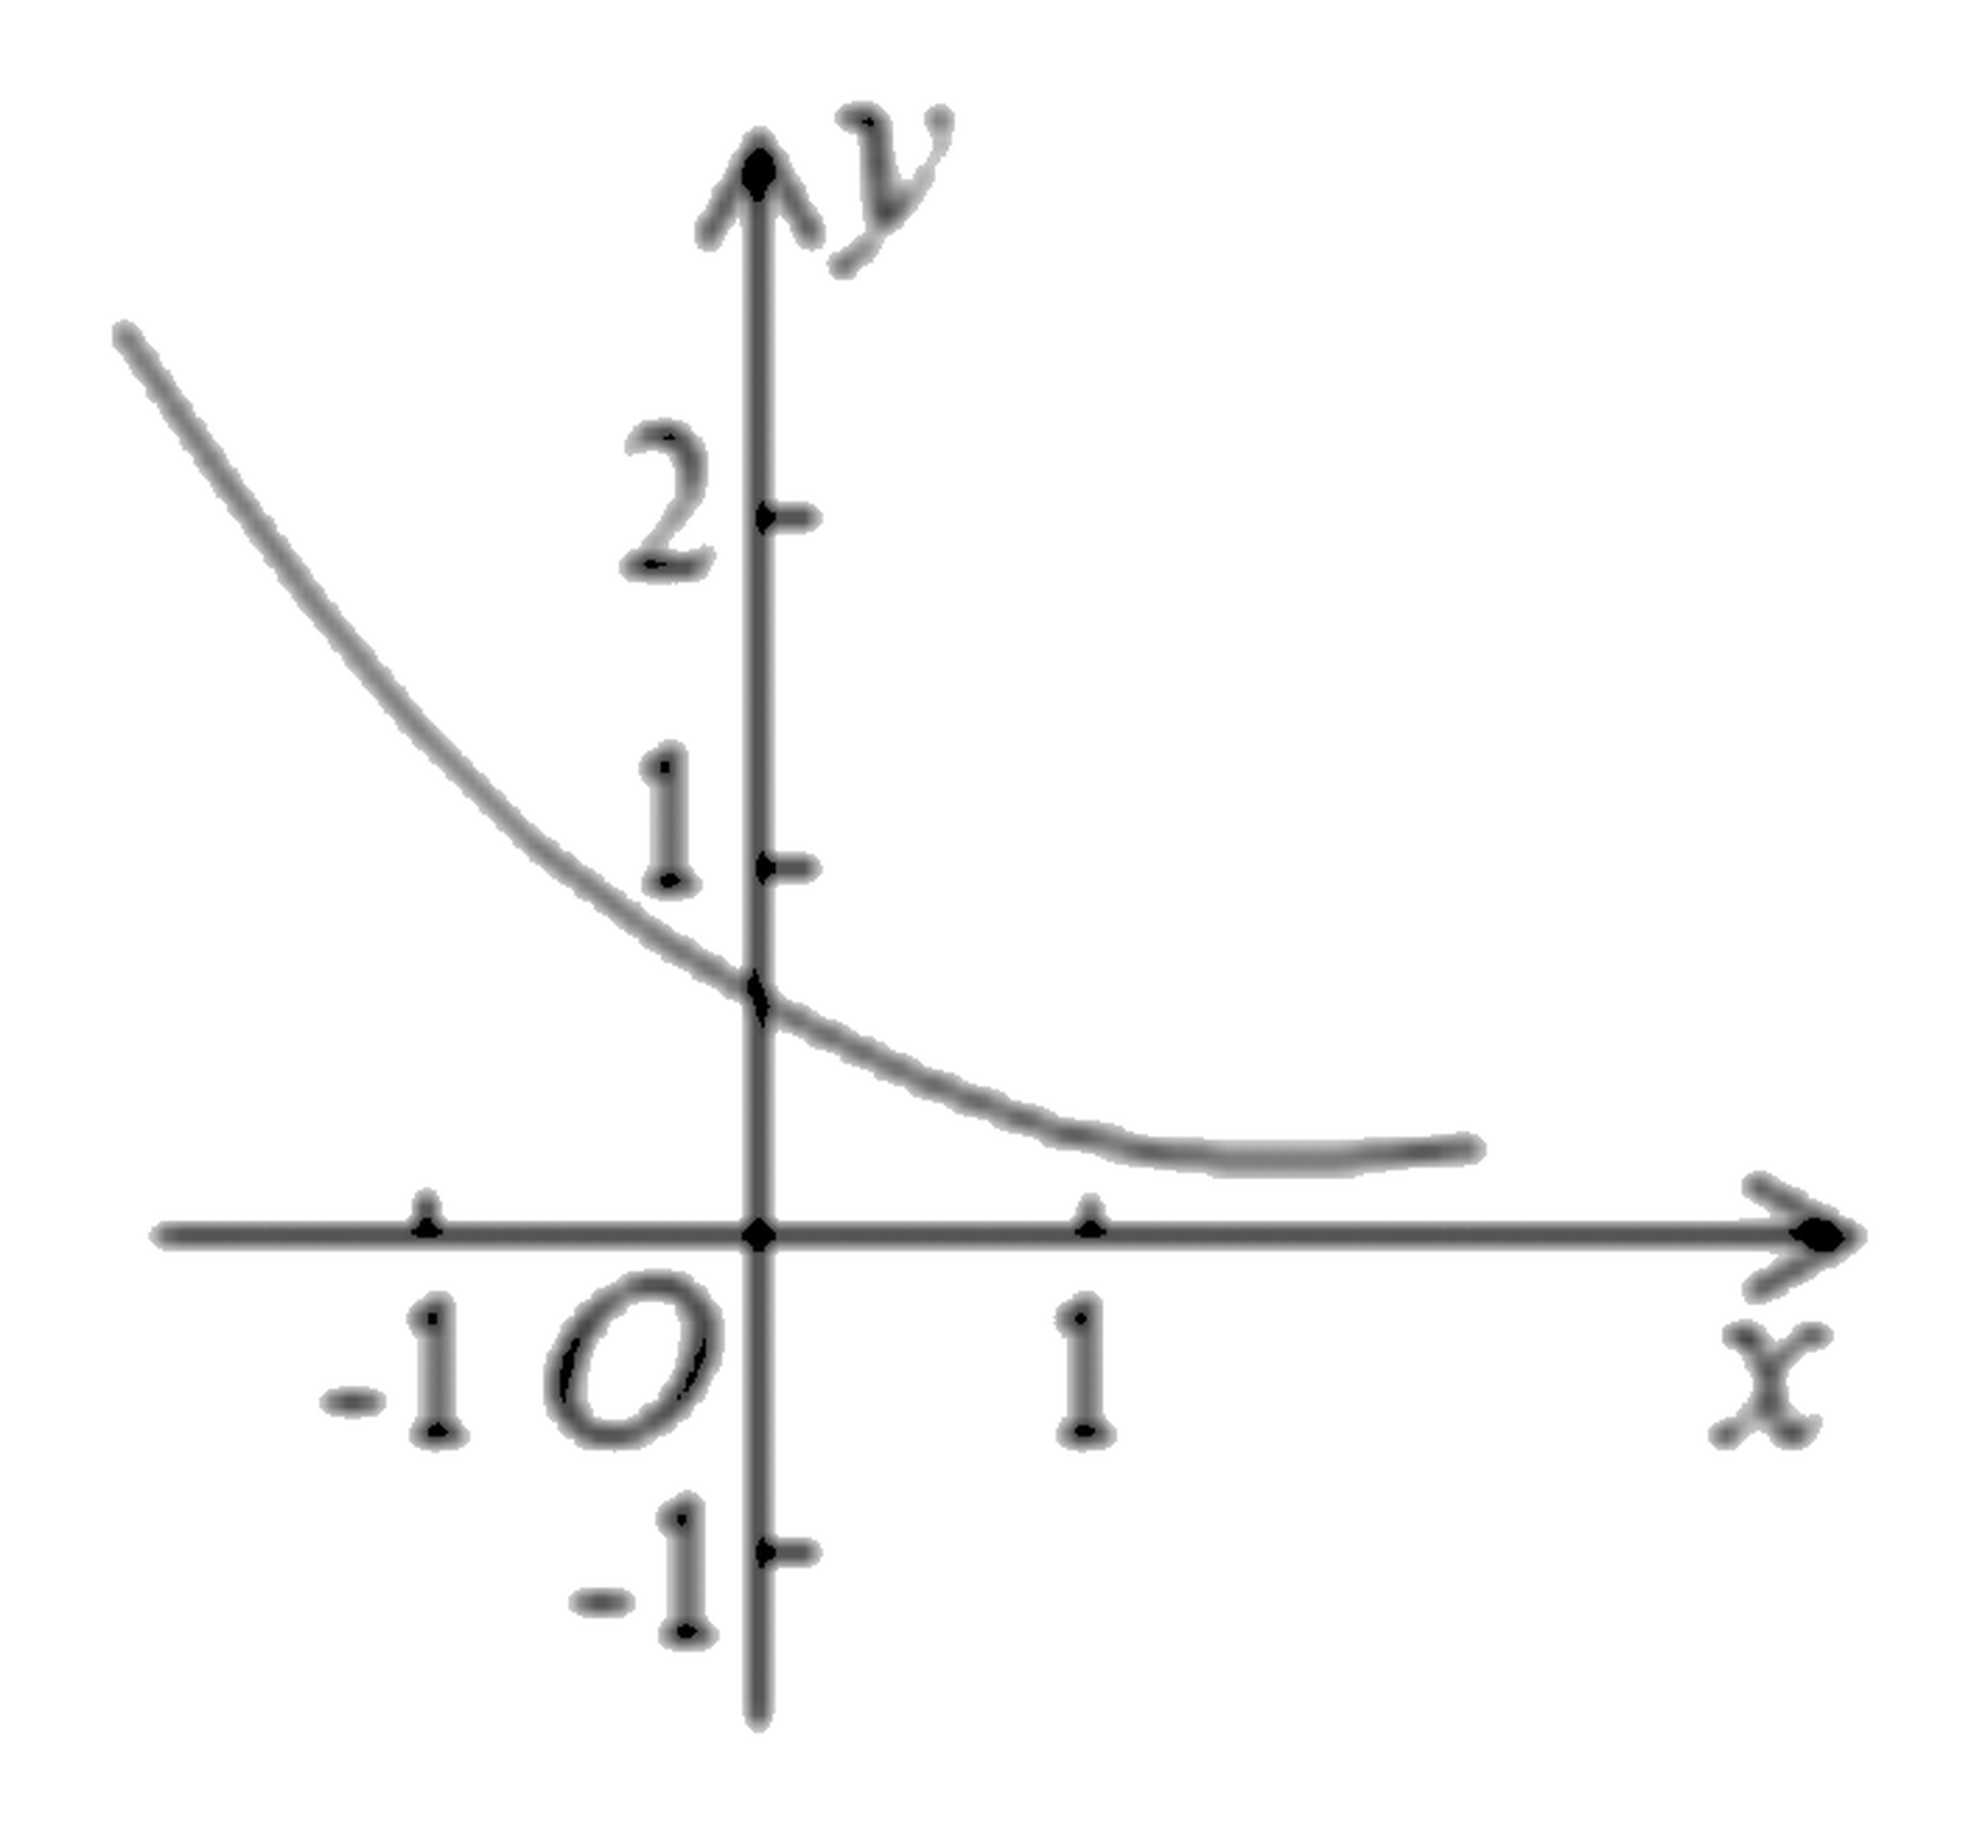
\includegraphics[width=0.30\textwidth]{figures/gao147_q15.png}
\end{center}

\ifanswer
\solbegin
\step{由图象从左到右下降得 $0<a<1$；}
\step{由图象与 $y$ 轴的交点得 $0<a^{-b}<1$，故 $b<0$；}
\step{故 $0<a<1$，$b<0$；故选 $D$.}
\solend
\fi

% === Q16 ===：位数新定义题（无弯引号，放大 04 页 z/q16_stem.png 确认）；四选项横排一行；解析 3 个印刷行
\item 数学运算是指在明晰运算对象的基础上，依据运算法则解决数学问题的素养. 因为运算，数的威力无限；没有运算，数就只是一个符号，对数运算与指数运算是两类重要的运算，对数的运算性质降低了运算的级别，简化了运算，在数学发展史上是伟大的成就. 而位数是指一个自然数有效位的个数，例如：$2^{10}=1024$，所以 $2^{10}$ 的位数为 4. 请你运用所学过的对数运算的知识，估计 $2025^{2026}$ 的位数是\mbox{（\quad）}

\keepwithprev
A. 6697\qquad B. 6698\qquad C. 6699\qquad D. 6700

\ifanswer
\solbegin
\step{设 $2025^{2026}=t$，所以 $\lg t=2026\lg2025$，}
\step{因为 $\lg2025\approx3.3064$，所以 $\lg t\approx6698.8$，}
\step{所以 $t\approx10^{6698.8}\in(10^{6698},10^{6699})$，所以 $2025^{2026}$ 的位数为 6699. 故选 $C$.}
\solend
\fi

\end{enumerate}

\bigsec{三、解答题}

\begin{enumerate}
\setcounter{enumi}{16}

% === Q17 ===：题干＋解析均在 04 页；集合描述竖线 \mid、描述内半角逗号照录；
% 空集 \varnothing、子集 \subseteq（放大 04 页 z/subset_04_q17b.png 确认带下划线）、数集 \R；
% 解析 5 个印刷行，首行末"所以 A=(-∞,-2)∪(3,+∞)"原卷无标点，照录不补
\item 已知集合 $A=\left\{x\mid \dfrac{x+2}{x-3}>0,x\in\R\right\}$，$B=\{x\mid \lvert x-2a\rvert\leqslant2,x\in\R\}$.

(1) 若 $a=1$，求 $A\cap B$；

(2) 若 $A\cap B=\varnothing$，求实数 $a$ 的取值范围.

\ifanswer
\solbegin
\step{由 $\dfrac{x+2}{x-3}>0$，得 $x<-2$ 或 $x>3$，所以 $A=(-\infty,-2)\cup(3,+\infty)$}
\step{(1) 当 $a=1$ 时，$B=\{x\mid \lvert x-2\rvert\leqslant2\}=[0,4]$，于是 $A\cap B=(3,4]$；}
\step{(2) $B=[2a-2,2a+2]$，}
\step{则 $A\cap B=\varnothing\Leftrightarrow[2a-2,2a+2]\subseteq[-2,3]\Leftrightarrow\begin{cases}2a-2\geqslant-2\\2a+2\leqslant3\end{cases}\Leftrightarrow0\leqslant a\leqslant\dfrac{1}{2}$，}
\step{所以实数 $a$ 的取值范围为 $\left[0,\dfrac{1}{2}\right]$.}
\solend
\fi

% === Q18 ===：氟化物／臭氧应用题；"氟化物""（如冰箱等）"全角夹注照录（放大 05 页 z/q18_line1.png 确认）；
% 关系式 $Q=Q_0e^{-0.0025t}$ 原卷独立一行，按一段照录；解析 6 个印刷行
\item 有些家用电器（如冰箱等）使用了氟化物，氟化物的释放破坏了大气上层的臭氧层，使臭氧含量 $Q$ 呈指数函数型变化，在氟化物排放量维持某种水平时，具有关系式

$Q=Q_0e^{-0.0025t}$，其中 $Q_0$ 是臭氧的初始量.

(1) 随时间 $t$ 的增加，臭氧的含量是增加还是减少？

(2) 试估计多少年以后将会有一半的臭氧消失.（用计算器计算）

\ifanswer
\solbegin
\step{(1) 对于函数 $Q=Q_0e^{-0.0025t}$，显然 $Q>0$，}
\step{任取 $t_1$、$t_2\in(0,+\infty)$，且 $t_1<t_2$，则 $t_2-t_1>0$，}
\step{所以 $\dfrac{Q_1}{Q_2}=\dfrac{Q_0e^{-0.0025t_1}}{Q_0e^{-0.0025t_2}}=e^{-0.0025(t_1-t_2)}=e^{0.0025(t_2-t_1)}>e^0=1$，所以 $Q_1>Q_2$，}
\step{故随着时间 $t$ 的增加，臭氧的含量是减少的；}
\step{(2) 令 $\dfrac{Q}{Q_0}=\dfrac{1}{2}$，即 $\dfrac{Q_0e^{-0.0025t}}{Q_0}=e^{-0.0025t}=\dfrac{1}{2}$，得 $-0.0025t=\ln\dfrac{1}{2}\approx-0.6931$，}
\step{解得 $t\approx277$，故估计 277 年以后将会有一半的臭氧消失.}
\solend
\fi

% === Q19 ===：题干用"图像"、解析两处用"图象"逐处照录不统一（05 页）；数集 \Z；
% 题干＋解析前 4 行在 05 页、解析后 3 行在 06 页；解析共 7 个印刷行
\item 已知幂函数 $f(x)=x^{-m^2+4m}(m\in\Z)$ 的图像关于 $y$ 轴对称，且在区间 $(0,+\infty)$ 上是严格增函数.

(1) 求 $m$ 的值；

(2) 求满足不等式 $(2a+1)^m<(a+1)^m$ 的实数 $a$ 的取值范围.

\ifanswer
\solbegin
\step{(1) 由题意得 $-m^2+4m>0$，解得 $0<m<4$，}
\step{因为 $m\in\Z$，所以 $m=1$ 或 $m=2$ 或 $m=3$.}
\step{当 $m=1$ 或 $m=3$ 时，$f(x)=x^3$，图象关于原点对称，不合题意；}
\step{当 $m=2$ 时，$f(x)=x^4$，图象关于 $y$ 轴对称，符合题意，所以 $m=2$.}
\step{(2) 代入 $m=2$，不等式为 $(2a+1)^2<(a+1)^2$，}
\step{得 $(2a+1)^2-(a+1)^2=a(3a+2)<0$，因此 $-\dfrac{2}{3}<a<0$，}
\step{所求范围为 $\left(-\dfrac{2}{3},0\right)$.}
\solend
\fi

% === Q20 ===：指数函数题，题干用"图像"；(3) 长求和式（分数 1/2026、1011/2026、2011/2026、
% 15/2026、1015/2026、2025/2026 放大 06 页 z/q20_sum_06a.png 确认）；题干在 06 页、
% 解析前 6 行在 06 页下半、后 6 行在 07 页上半；解析共 12 个印刷行
\item 已知指数函数 $y=a^x$（$a>0,a\ne1$）的图像经过点 $(1,4)$.

(1) 求实数 $a$ 的值；

(2) 若 $f(x)=(a^x)^2-2\cdot a^x-8$，当 $x\in\R$ 时，不等式 $f(x)>m\cdot4^x-12$ 恒成立，求 $m$ 的取值范围；

(3) 记 $g(x)=\dfrac{1}{a^x+2}$，求证：$g(x)+g(1-x)$ 为定值，并求 $g(0)+g\left(\dfrac{1}{2026}\right)+g\left(\dfrac{1011}{2026}\right)+g\left(\dfrac{2011}{2026}\right)+g\left(\dfrac{1}{2}\right)+g\left(\dfrac{15}{2026}\right)+g\left(\dfrac{1015}{2026}\right)+g\left(\dfrac{2025}{2026}\right)+g(1)$ 的值.

\ifanswer
\solbegin
\step{(1) 将 $(1,4)$ 代入 $y=a^x$，得 $a^1=4$，即 $a=4$.}
\step{(2) 令 $t=4^x$，当 $x\in\R$ 时，$t$ 取遍所有正实数.}
\step{原不等式等价于 $t^2-2t-8>mt-12\Leftrightarrow m<t+\dfrac{4}{t}-2$，}
\step{由基本不等式，$t+\dfrac{4}{t}-2\geqslant2\sqrt{t\cdot\dfrac{4}{t}}-2=2$，}
\step{当且仅当 $t=\dfrac{4}{t}$，即 $t=2$ 时取等号，}
\step{因此原不等式恒成立的充要条件为 $m<2$，即 $m\in(-\infty,2)$.}
\step{(3) 对任意 $x\in\R$，令 $t=4^x>0$，则 $4^{1-x}=\dfrac{4}{t}$，}
\step{从而 $g(x)+g(1-x)=\dfrac{1}{t+2}+\dfrac{1}{\dfrac{4}{t}+2}=\dfrac{1}{t+2}+\dfrac{t}{2(t+2)}=\dfrac{1}{2}$，}
\step{因此 $g(x)+g(1-x)$ 为定值 $\dfrac{1}{2}$.}
\step{原式中，0 与 1、$\dfrac{1}{2026}$ 与 $\dfrac{2025}{2026}$、$\dfrac{1011}{2026}$ 与 $\dfrac{1015}{2026}$、$\dfrac{2011}{2026}$ 与 $\dfrac{15}{2026}$}
\step{分别配对，每对函数值之和均为 $\dfrac{1}{2}$，且 $g\left(\dfrac{1}{2}\right)=\dfrac{1}{4^{\frac12}+2}=\dfrac{1}{4}$，}
\step{所以所求和为 $4\cdot\dfrac{1}{2}+\dfrac{1}{4}=\dfrac{9}{4}$.}
\solend
\fi

% === Q21 ===：不动点新定义题；题干在 07 页、解析续 08／09 页，共 20 个印刷行；
% 判别式两形混用：08 页 (2) cases 内等腰偏高 \Delta、09 页 (3) 扁等边 \triangle，逐处照录不统一
% （放大 /tmp/gao147/z/delta_vs_triangle.png 并排确认）；数集 \R；\forall 照录；
% 第 6—8 行是原卷一个长算式折成的三个印刷行，按印刷行分三条 \step、不并折行
\item 对于二次函数 $y=mx^2+nx+t(m\ne0)$，若存在 $x_0\in\R$，使得 $mx_0^2+nx_0+t=x_0$ 成立，则称 $x_0$ 为二次函数 $y=mx^2+nx+t(m\ne0)$ 的不动点.

(1) 求二次函数 $y=x^2-x-3$ 的不动点；

(2) 若二次函数 $y=2x^2-(3+a)x+a-1$ 有两个不相等的不动点 $x_1$、$x_2$，且 $x_1$、$x_2>0$，求 $\dfrac{x_1}{x_2}+\dfrac{x_2}{x_1}$ 的最小值；

(3) 若对任意实数 $b$，二次函数 $y=ax^2+(b+1)x+(b-1)(a\ne0)$ 恒有不动点，求 $a$ 的取值范围.

\ifanswer
\solbegin
\step{(1) 令 $x^2-x-3=x$，即 $x^2-2x-3=0$，即 $(x-3)(x+1)=0$，}
\step{解得 $x_1=-1$，$x_2=3$，所以不动点为 $-1$ 和 $3$.}
\step{(2) 由题意，$2x^2-(3+a)x+a-1=x$ 有两个不相等的正实数根，}
\step{即方程 $2x^2-(4+a)x+a-1=0$ 有两个不相等的正实数根，}
\step{所以 $\begin{cases}\Delta=(4+a)^2-8(a-1)>0\\x_1+x_2=\dfrac{4+a}{2}>0\\x_1\cdot x_2=\dfrac{a-1}{2}>0\end{cases}$，解得 $a>1$，}% 判别式原卷印等腰偏高粗三角 $\Delta$（放大 08 页 z/delta_08_q21cases.png）
\step{所以 $\dfrac{x_1}{x_2}+\dfrac{x_2}{x_1}=\dfrac{x_1^2+x_2^2}{x_1\cdot x_2}=\dfrac{(x_1+x_2)^2-2x_1\cdot x_2}{x_1\cdot x_2}=\dfrac{(x_1+x_2)^2}{x_1\cdot x_2}-2$}
\step{$=\dfrac{\left(\dfrac{4+a}{2}\right)^2}{\dfrac{a-1}{2}}-2=\dfrac{\dfrac{(a+4)^2}{4}}{\dfrac{a-1}{2}}-2=\dfrac{(a-1+5)^2}{2(a-1)}-2$}
\step{$=\dfrac{(a-1)^2+10(a-1)+25}{2(a-1)}-2=\dfrac{a-1}{2}+\dfrac{25}{2(a-1)}+3$.}
\step{因为 $a>1$，所以 $a-1>0$，}
\step{所以 $\dfrac{a-1}{2}+\dfrac{25}{2(a-1)}+3\geqslant2\sqrt{\dfrac{a-1}{2}\cdot\dfrac{25}{2(a-1)}}+3=8$，}
\step{当且仅当 $\dfrac{a-1}{2}=\dfrac{25}{2(a-1)}$，即 $a=6$ 时等号成立，}
\step{所以 $\dfrac{x_1}{x_2}+\dfrac{x_2}{x_1}$ 的最小值为 $8$.}
\step{(3) 设 $f(x)=ax^2+(b+1)x+b-1$，}
\step{则方程 $f(x)=x$，可化为 $ax^2+(b+1)x+b-1=x$，}
\step{即 $ax^2+bx+b-1=0$，}
\step{由题意得一元二次方程 $ax^2+bx+b-1=0$ 有解，又 $a\ne0$，}
\step{所以方程 $ax^2+bx+b-1=0$ 的判别式 $\triangle=b^2-4a(b-1)\geqslant0$，}% 判别式原卷印扁等边细线三角 $\triangle$（放大 09 页 z/triangle_09_q21.png），与 (2) 高 $\Delta$ 混用、照录不统一
\step{即 $b^2-4ab+4a\geqslant0$，则该不等式对 $\forall b\in\R$ 恒成立，}
\step{则 $(4a)^2-4\times4a\leqslant0$，且 $a\ne0$，解得 $0<a\leqslant1$，}
\step{所以实数 $a$ 的取值范围是 $(0,1]$.}
\solend
\fi

\end{enumerate}

\end{document}
"
%
% ① 原始材料：微信公众号"魔都数学加油站"文章，连载"27学年高一147"，原文标题
% "27学年高一147——2026-2027年上海市华师大三附中高一上期中"；
% 原文链接：https://mp.weixin.qq.com/s/X_gPW1JWoTAl2Bky_xEEGw 。
% 正文为 9 张 PNG 页（01/06/08/09 为 2560×3620，02/03/04/05/07 为 4762×6735，
% 同一篇各页分辨率混排，逐页按各自分辨率裁图核对，别按预览比例换算裁框）。
% 体例：混合体例讲评版——19 题中 Q4/Q5/Q7/Q9 只印【答案】、无【解析】，其余 15 题印
% 【解析】（逐题核实，见 ② ②）。题目、答案、解析均据原图转录；卷面粉红色水印
% "魔都数学加油站"及公众号页脚未录入。
% 全卷插图清单（逐页通读 9 页确认）：仅 1 处题目配图——
%   · Q15 递减指数函数小坐标系（03 页右侧：坐标轴、y 轴刻度 2/1/-1、x 轴刻度 -1/1、
%     原点 O、x/y 轴标），为"图像如图所示"的题目配图（选择题选项旁），三版都出；
%     裁自 03 页去粉色水印、去色、4× LANCZOS 放大存 figures/gao147_q15.png；
%   其余 8 页逐页确认无其它题目配图、无【解析】内配图、无表格，
%   亦无"题干写如图而源码漏图"一处；Q12/Q17/Q21 的 cases 块为数学块（非图）。
%
% 卷首标题：原卷印作"2026-2027 年华师大三附中高一上期中"，年份区间按全稿惯例排 en dash；
% 原卷卷面未印副标题，本稿按同期中卷（高一140／141／143／144／145／146）知识模块口径
% 补出"集合与常用逻辑用语、不等式、函数"。
%
% 题号体例（逐页核实定稿）：本卷共 19 题——一、填空题 3—12（10 题）、
% 二、选择题 13—16（4 题）、三、解答题 17—21（5 题）。
% 三节分别 \setcounter{enumi}{2}／{12}／{16}。原卷从第 3 题起、无第 1、2 题，
% 本稿保留原题号；全卷无附加题节（Q21 解析末行"所以实数 a 的取值范围是 (0,1]."
% 为全卷收尾，09 页下半仅水印、无正文）。
%
% ② 与原卷的排版差异：
%   ① 原文从第 3 题起，本稿保留原题号；共 19 题三节；
%   ② 混合体例：原卷 Q4/Q5/Q7/Q9 只印【答案】、无【解析】（分别为 a≤0、(-1,2)、
%      真、(-∞,1)），按 高一140 第 5 题／高一145 Q3 成例提 \ans{}、不补造解析；
%      其余 15 题印【解析】，用 \solbegin…\solend，选择题答案在解析末句"故选 X"
%      （Q13 选 B、Q14 选 B、Q15 选 D、Q16 选 C，逐个放大原图核实）、题干括号
%      \mbox{（\quad）} 留空、不另提 \ans{}；填空／解答答案落在解析里；
%      答案版【答案】/【解析】标记数 = 19（4 个 \ans ＋ 15 个 \solbegin）= 全卷题数；
%   ③ 原卷卷面未印副标题，本稿按知识模块口径补出；
%   ④ 原卷填空横线按全稿惯例排 \blankline[4.4em]；选择题括号排 \mbox{（\quad）}、
%      选项段前按惯例加 \keepwithprev；Q14／Q15 四选项为 2×2 两印刷行（A/B 一行、
%      C/D 一行），用空行分段照录（非一行 \qquad、亦非竖排四行）；解答题不留作答区、
%      不加 \anspace（原卷为讲评版，与 129／131／132／133／136／140／141／143／144／145／146 同）；
%   ⑤ 数集：Q4"A∪B=R"、Q13"f(x)=x^3 在 R 上严格增"、Q17"x∈R"两处、
%      Q20"x∈R"两处、Q21"x_0∈R""∀b∈R"原卷印斜体或黑板粗体 R，按全稿惯例统一改 \R；
%      Q19"m∈Z"改 \Z；本卷未出现 N（\N^* 无对应处）。绝对值排 \lvert…\rvert，
%      集合描述竖线排 \mid；不等号按全稿惯例排 \leqslant／\geqslant（原卷印 \le／\ge 形，
%      【答案】a≤0 亦排 \leqslant）；空集 \varnothing（Q17 两处）；
%      子集 \subseteq（Q17 带下划线，放大 04 页确认）；本卷未出现 \subset／\subsetneq，
%      亦未出现补集上划线 \overline{}；\left…\right 不得拆到不同 $…$ 组；
%   ⑥ 子题标号 (1)(2)(3) 半角括号照录；cases 块整体算一个印刷行（Q3、Q12 一行内
%      两个 cases、Q17、Q21(2)）；本卷解析内无圈数字①②③（无 \text{①} 需求）；
%      数学式内 CJK 用 \text{}（本卷未见）；
%   ⑦ 题干中的中文弯引号按原卷照录：Q7 命题"若 A∪B=B，则 A∩B=A"与
%      (填 " 真 " 或 " 假 ")、Q10 (填 ">" "<" "≤" "或≥")，含引号内空格；
%      注释内一律 ASCII 引号；Q16 位数新定义题逐字放大确认无弯引号
%      （交办提示的"Q16 新定义题"举例未在本卷出现），未补造引号；
%   ⑧ 半角逗号在数学组之间是全稿惯例、非笔误（Q4"$A=(-\infty,0],B=[a,+\infty)$"、
%      Q5"$(a>0,a\ne1)$"、Q17 集合描述内"$>0,x\in R$""$\leqslant2,x\in R$"、
%      Q20 题干"$(a>0,a\ne1)$"、Q21"$y=mx^2+nx+t(m\ne0)$"等），逐处照录别改全角；
%      行末西文句点照录为 ASCII `.`；行中全角逗号／顿号照录；
%      Q7／Q10"(填…)"为半角括号、Q18"（如冰箱等）"为全角括号，逐处照录不统一；
%   ⑨ "图像／图象"逐处照录不统一：题干 5 处用"图像"（Q5"图像恒过定点"、
%      Q9"图像位于直线 y=x 的下方"、Q15"的图像如图所示"、Q19"的图像关于 y 轴对称"、
%      Q20"的图像经过点"），解析 4 处用"图象"（Q15"由图象从左到右下降"
%      "由图象与 y 轴的交点"、Q19"图象关于原点对称""图象关于 y 轴对称"），逐处核、不统一；
%   ⑩ 判别式 Δ/△ 混用是照录项：Q21(2) 解析 cases 块"Δ=(4+a)²−8(a−1)>0"
%      印等腰偏高粗三角 \Delta，Q21(3) 解析"判别式△=b²−4a(b−1)≥0"
%      印扁等边细线三角 \triangle，逐处放大判断、照录不得统一
%      （参照 高一142／144／145 头注④口径，详见 ④）；
%   ⑪ 一条 \step = 原卷解析的一个印刷行，cases 块整体算一个印刷行；别把原卷折行
%      并起来、别把一行拆多条。Q10 七行（跨 01→02 页）、Q12 七行（含一行两 cases）、
%      Q20 十二行（含"原式中…2011/2026 与 15/2026／分别配对…"折行两行）、
%      Q21 二十行（含第 6—8 行一个长算式折成三印刷行、含 cases）均按印刷行逐条断，
%      不丢行；
%   ⑫ 配图：逐页通读 9 页确认全卷仅 Q15 一处题目配图（见 ①），三版都出、
%      \includegraphics[width=0.30\textwidth]；图块较小，未加 \needvspace 大图块守卫
%      （仅 \bigsec 自带 \needvspace{3\baselineskip}）；三版切页审计均"合计异常：无"；
%   ⑬ 跨页续印按题合并：Q3—Q9 在 01 页（Q10 题干在 01 页末、解析首行亦在 01 页末）；
%      Q10 解析续 02 页 6 行、Q11 在 02 页、Q12 题干＋解析前 4 行在 02 页
%      （解析续 03 页 3 行）；"二、选择题"标题与 Q13、Q14、Q15 题干＋解析前 2 行在 03 页
%      （Q15 配图在 03 页右侧）；Q15 解析末行与 Q16、"三、解答题"标题、Q17 在 04 页；
%      Q18 在 05 页、Q19 题干＋解析前 4 行在 05 页（解析续 06 页 3 行）；
%      Q20 题干＋解析前 6 行在 06 页（解析续 07 页 6 行）、Q21 题干＋解析前 3 行在 07 页；
%      Q21 解析续 08 页 13 行、续 09 页 4 行（09 页下半仅水印、无正文）。
%      本稿按题连排，不丢行、不并折行；
%   ⑭ 原卷解析内无红色"法一／法二"之类小标题，故本卷无 \stepm；
%      水印"魔都数学加油站"红色不录入。
%
% ③ 行数复核：一条 \step／\stepm = 原卷解析的一个印刷行，cases 块作一个印刷行计。
%   逐题数（主会话逐页核对定稿）：Q3：1；Q4：0（只印【答案】、提 \ans{}，不计入 \step 账）；
%   Q5：0；Q6：1；Q7：0；Q8：2；Q9：0；Q10：7；Q11：4；Q12：7；Q13：6；Q14：4；
%   Q15：3；Q16：3；Q17：5；Q18：6；Q19：7；Q20：12；Q21：20。
%   合计 88 条 \step（本卷无 \stepm：解析内无红色"法一／法二"类小标题），
%   与原卷逐题印刷行相等。全卷 15 题设 \solbegin…\solend ＋ 4 题一处 \ans{}，
%   答案版【答案】/【解析】标记数 = 19 = 全卷题数。
%
% ④ 判别式／子集符号结论（逐处放大原图照录、不得统一，主会话像素级复核）：
%   判别式全卷 2 处、两形混用逐处照录不统一（参照 高一142／144 头注④口径）：
%     · Q21(2) 解析 cases 块"Δ=(4+a)²−8(a−1)>0" 原卷印等腰偏高粗三角
%       （高>宽、粗笔画），照录 \Delta（放大 08 页 /tmp/gao147/z/delta_08_q21cases.png
%       与 z/delta_vs_triangle.png 左图确认）；
%     · Q21(3) 解析"判别式△=b²−4a(b−1)≥0" 原卷印扁等边细线三角
%       （宽≈高、细线），照录 \triangle（放大 09 页 /tmp/gao147/z/triangle_09_q21.png
%       与 z/delta_vs_triangle.png 右图并排确认）。
%   子集／补集：Q17 解析"[2a−2,2a+2]⊆[−2,3]" 原卷印带下划线 ⊆，照录 \subseteq
%     （放大 04 页 /tmp/gao147/z/subset_04_q17b.png 确认）；Q17"A∩B=∅"空集 \varnothing；
%     集合描述竖线 \mid（Q10 M、Q12 解集、Q17 A/B）；并集 \cup（Q4、Q17）、
%     交集 \cap（Q7、Q17）、不属于 \notin（Q10）；数集 \R／\Z 归一见 ② ⑤。
%   本卷未出现 \subset／\subsetneq，未出现补集上划线 \overline{}。
%
% ⑤ 存疑照录（放大原图确认，照录未改、正文对应处另有 % 注）：
%   1. Q4/Q5/Q7/Q9 只印【答案】、无【解析】，按成例提 \ans{}、不补造解析
%      （混合体例逐题核实，见 ② ②）。
%   2. Q21(2) 判别式高 \Delta 与 Q21(3) 判别式扁 \triangle 两形混用，
%      逐处照录不统一（见 ④）。
%   3. "图像／图象"题干 5 处"图像"、解析 4 处"图象"，逐处照录不统一（见 ② ⑨）。
%   4. Q7／Q10"(填…)"半角括号与 Q18"（如冰箱等）"全角括号，逐处照录不统一。
%   5. Q16 位数新定义题逐字放大确认无弯引号（交办提示的"Q16 新定义题"举例
%      未在本卷出现），未补造引号；全卷弯引号仅 Q7、Q10 两处。
%   6. Q17 解析首行末"所以 A=(-∞,-2)∪(3,+∞)"、Q20(3) 解析"…2011/2026 与 15/2026"
%      行末原卷均无标点，照录未补；Q21(2) 第 6—8 行一个长算式折成三印刷行，
%      按印刷行分三条 \step、不并折行。
%   全卷除此 6 类外未发现其它笔误／自相矛盾处。
%
% ⑥ 跨页续印按题合并说明：见 ② ⑬。
%
\documentclass[a4paper,11pt]{article}
\usepackage{common}

\begin{document}

\examtitlest[3]{2026--2027 年华师大三附中高一上期中}{集合与常用逻辑用语、不等式、函数}

\bigsec{一、填空题}

\begin{enumerate}
\setcounter{enumi}{2}

% === Q3 ===：印【解析】，1 个印刷行（cases 块整体算一行）
\item 函数 $y=(a^2-5a+7)a^x+6-2a$ 是指数函数，则 $a$ 的值为\blankline[4.4em].

\ifanswer
\solbegin
\step{由题意得 $\begin{cases}a^2-5a+7=1\\6-2a=0\end{cases}$，解得 $a=3$.}
\solend
\fi

% === Q4 ===：原卷只印【答案】、无【解析】，按 高一140 第 5 题／高一145 Q3 成例提 \ans{}、不补造解析；
% 题干数学组内半角逗号 $A=(-\infty,0],B=[a,+\infty)$ 照录（放大 01 页 z/q4_stem.png 确认）
\item 已知 $A=(-\infty,0],B=[a,+\infty)$，且 $A\cup B=\R$，则实数 $a$ 的取值范围为\blankline[4.4em].

\ifanswer
\ans{$a\leqslant0$}
\fi

% === Q5 ===：只印【答案】；题干"图像"照录（放大 01 页 z/q5_stem.png 确认）；
% 数学组内半角逗号 $(a>0,a\ne1)$ 照录
\item 函数 $y=a^{x+1}+1(a>0,a\ne1)$ 的图像恒过定点\blankline[4.4em].

\ifanswer
\ans{$(-1,2)$}
\fi

% === Q6 ===：印【解析】，1 个印刷行
\item 已知方程 $x^2+2x-4=0$ 的两个根为 $x_1$、$x_2$，则 $x_1^2+x_2^2$ 的值为\blankline[4.4em].

\ifanswer
\solbegin
\step{$x_1^2+x_2^2=(x_1+x_2)^2-2x_1x_2=4+8=12$.}
\solend
\fi

% === Q7 ===：只印【答案】；中文弯引号"若 A∪B=B，则 A∩B=A"与(填 " 真 " 或 " 假 ")内的空格照录
% （放大 01 页 z/q7_quotes_7x.png、z/q7_tail.png 确认，括号为半角）
\item 命题 “若 $A\cup B=B$，则 $A\cap B=A$” 为\blankline[4.4em]命题(填 “ 真 ” 或 “ 假 ”).

\ifanswer
\ans{真}
\fi

% === Q8 ===：印【解析】，2 个印刷行；不等号按全稿惯例 \geqslant／\leqslant
\item 已知正实数 $a$、$b$ 满足 $a+4b=1$，则 $ab$ 的最大值为\blankline[4.4em].

\ifanswer
\solbegin
\step{$a+4b\geqslant2\sqrt{a\cdot4b}\Rightarrow ab\leqslant\dfrac{1}{16}$，当且仅当 $a=4b=\dfrac{1}{2}$ 时取等号，}
\step{则 $ab$ 的最大值为 $\dfrac{1}{16}$.}
\solend
\fi

% === Q9 ===：只印【答案】；题干"图像"照录（放大 01 页 hi_01_2 确认）
\item 若幂函数 $y=x^s$ 在 $x>1$ 时的图像位于直线 $y=x$ 的下方，则 $s$ 的取值范围是\blankline[4.4em].

\ifanswer
\ans{$(-\infty,1)$}
\fi

% === Q10 ===：印【解析】，共 7 个印刷行（题在 01 页末起 1 行、续 02 页 6 行）；
% 题干跨两印刷行"则 |ab|+1 ____ |a|+|b|（填…）"按一句连排；(填…)为半角括号、引号内空格照录
\item 已知不等式 $\lvert2x+1\rvert+\lvert2x-1\rvert<4$ 的解集为 $M$. 设实数 $a\in M$，$b\notin M$，则 $\lvert ab\rvert+1$\blankline[4.4em] $\lvert a\rvert+\lvert b\rvert$(填 “$>$”，“$<$”，“$\leqslant$” “或$\geqslant$”).

\ifanswer
\solbegin
\step{当 $x<-\dfrac{1}{2}$ 时，不等式化为 $-2x-1+1-2x<4$，即 $x>-1$，所以 $-1<x<-\dfrac{1}{2}$；}
\step{当 $-\dfrac{1}{2}\leqslant x\leqslant\dfrac{1}{2}$ 时，不等式化为 $2x+1-2x+1<4$，即 $2<4$，所以 $-\dfrac{1}{2}\leqslant x\leqslant\dfrac{1}{2}$；}
\step{当 $x>\dfrac{1}{2}$ 时，不等式化为 $2x+1+2x-1<4$，即 $x<1$，所以 $\dfrac{1}{2}<x<1$；}
\step{综上，$M=\{x\mid -1<x<1\}$.}
\step{因为 $a\in M$，$b\notin M$，所以 $\lvert a\rvert<1$，$\lvert b\rvert\geqslant1$.}
\step{而 $\lvert ab\rvert+1-(\lvert a\rvert+\lvert b\rvert)=\lvert ab\rvert+1-\lvert a\rvert-\lvert b\rvert=(\lvert a\rvert-1)(\lvert b\rvert-1)$，}
\step{所以 $\lvert ab\rvert+1\leqslant\lvert a\rvert+\lvert b\rvert$.}
\solend
\fi

% === Q11 ===：印【解析】，4 个印刷行（02 页）
\item 已知 $m>1$，$n>1$，$\lg m=\log_n100$，则 $mn$ 的最小值为\blankline[4.4em].

\ifanswer
\solbegin
\step{由 $m>1$，$n>1$，得 $\lg m>0$，$\lg n>0$，}
\step{因为 $\lg m=\log_n100=\dfrac{\lg100}{\lg n}=\dfrac{2}{\lg n}$，所以 $\lg m\cdot\lg n=2$，}
\step{所以 $\lg(mn)=\lg m+\lg n\geqslant2\sqrt{\lg m\cdot\lg n}=2\sqrt2$，}
\step{当且仅当 $m=n=10^{\sqrt2}$ 时取等号，则 $mn\geqslant10^{2\sqrt2}$，即 $mn$ 的最小值为 $10^{2\sqrt2}$.}
\solend
\fi

% === Q12 ===：印【解析】，共 7 个印刷行（02 页 4 行、03 页 3 行）；
% 第 3 行"则 [cases]，得 [cases]，"两个 cases 块同属一个印刷行，整体作一条 \step（照 高一146 Q11 成例）
\item 已知关于 $x$ 的不等式 $ax^2+bx+c\leqslant1$ 的解集为 $\{x\mid -1\leqslant x\leqslant3\}$. 若关于 $x$ 的不等式 $ax^2+(b-1)x+c-2\leqslant0$ 有且仅有 8 个整数解，则实数 $a$ 的取值范围是\blankline[4.4em].

\ifanswer
\solbegin
\step{由已知关于 $x$ 的不等式 $ax^2+bx+c\leqslant1$ 的解集为 $\{x\mid -1\leqslant x\leqslant3\}$，}
\step{得 $a>0$，且方程 $ax^2+bx+c-1=0$ 的两根分别为 $-1$ 和 $3$，}
\step{则 $\begin{cases}-1+3=-\dfrac{b}{a}\\-1\times3=\dfrac{c-1}{a}\end{cases}$，得 $\begin{cases}b=-2a\\c=1-3a\end{cases}$，}
\step{不等式 $ax^2+(b-1)x+c-2\leqslant0$ 等价于 $ax^2-(2a+1)x-(3a+1)\leqslant0$，}
\step{即 $\left[x-\left(3+\dfrac{1}{a}\right)\right](x+1)\leqslant0$，解得 $-1\leqslant x\leqslant3+\dfrac{1}{a}$，}
\step{因为关于 $x$ 的不等式 $ax^2+(b-1)x+c-2\leqslant0$ 有且仅有 8 个整数解，}
\step{因此 $6\leqslant3+\dfrac{1}{a}<7$，即 $3\leqslant\dfrac{1}{a}<4$，解得 $\dfrac{1}{4}<a\leqslant\dfrac{1}{3}$，所以 $a$ 的取值范围为 $\left(\dfrac{1}{4},\dfrac{1}{3}\right]$.}
\solend
\fi

\end{enumerate}

\bigsec{二、选择题}

\begin{enumerate}
\setcounter{enumi}{12}

% === Q13 ===：题干＋选项＋解析均在 03 页；四选项横排一行；解析 6 个印刷行，末句"故选 B."
\item $a<b<0$，则下列不等式能成立的是\mbox{（\quad）}

\keepwithprev
A. $\dfrac{a}{b}<1$\qquad B. $\lvert a\rvert>-b$\qquad C. $\dfrac{1}{a}<\dfrac{1}{b}$\qquad D. $b^3<a^3$

\ifanswer
\solbegin
\step{对于 $A$，令 $a=-4$，$b=-3$，满足 $a<b<0$，但 $\dfrac{a}{b}>1$，故 $A$ 错误，}
\step{对于 $B$，因为 $a<b<0$，所以 $-a>-b>0$，即 $\lvert a\rvert>-b$，故 $B$ 正确，}
\step{对于 $C$，令 $a=-4$，$b=-3$，满足 $a<b<0$，但 $\dfrac{1}{a}>\dfrac{1}{b}$，故 $C$ 错误，}
\step{对于 $D$，$f(x)=x^3$ 在 $\R$ 上严格增，因为 $a<b$，所以 $f(a)<f(b)$，}
\step{即 $a^3<b^3$，故 $D$ 错误.}
\step{故选 $B$.}
\solend
\fi

% === Q14 ===：四选项原卷为 2×2 两印刷行（A/B 一行、C/D 一行），用空行分段照录；解析 4 个印刷行
\item 已知 $a$、$b$ 为实数，若 $\alpha:ab=0$，$\beta:a^2+\sqrt{b}=0$，则 $\alpha$ 是 $\beta$ 的\mbox{（\quad）}

\keepwithprev
A. 充分不必要条件\qquad\qquad B. 必要不充分条件

C. 充要条件\qquad\qquad D. 既不充分也不必要条件

\ifanswer
\solbegin
\step{$\beta:a^2+\sqrt{b}=0$，所以 $a=0$ 且 $b=0$，}
\step{由 $a=0$，$b=0\Rightarrow ab=0$，反之不成立.}
\step{所以 $ab=0$ 是 $a=0$，$b=0$ 的必要不充分条件，即 $\alpha$ 是 $\beta$ 的必要不充分条件，}
\step{故选 $B$.}
\solend
\fi

% === Q15 ===：题目配图（03 页右侧小坐标系），三版都出；题干用"图像"、解析用"图象"逐处照录；
% 四选项 2×2 两印刷行；解析 3 个印刷行（03 页 2 行、04 页 1 行，末句"故选 D."与前行同一印刷行）
\item 函数 $f(x)=a^{x-b}$ 的图像如图所示，其中 $a$、$b$ 为常数，则下列结论正确的是\mbox{（\quad）}

\keepwithprev
A. $a>1$，$b<0$\qquad\qquad B. $a>1$，$b>0$

C. $0<a<1$，$b>0$\qquad\qquad D. $0<a<1$，$b<0$

\begin{center}
% 递减指数函数小坐标系图取 03 页右侧，去粉色水印、去色、4× LANCZOS 放大；题目配图三版都出
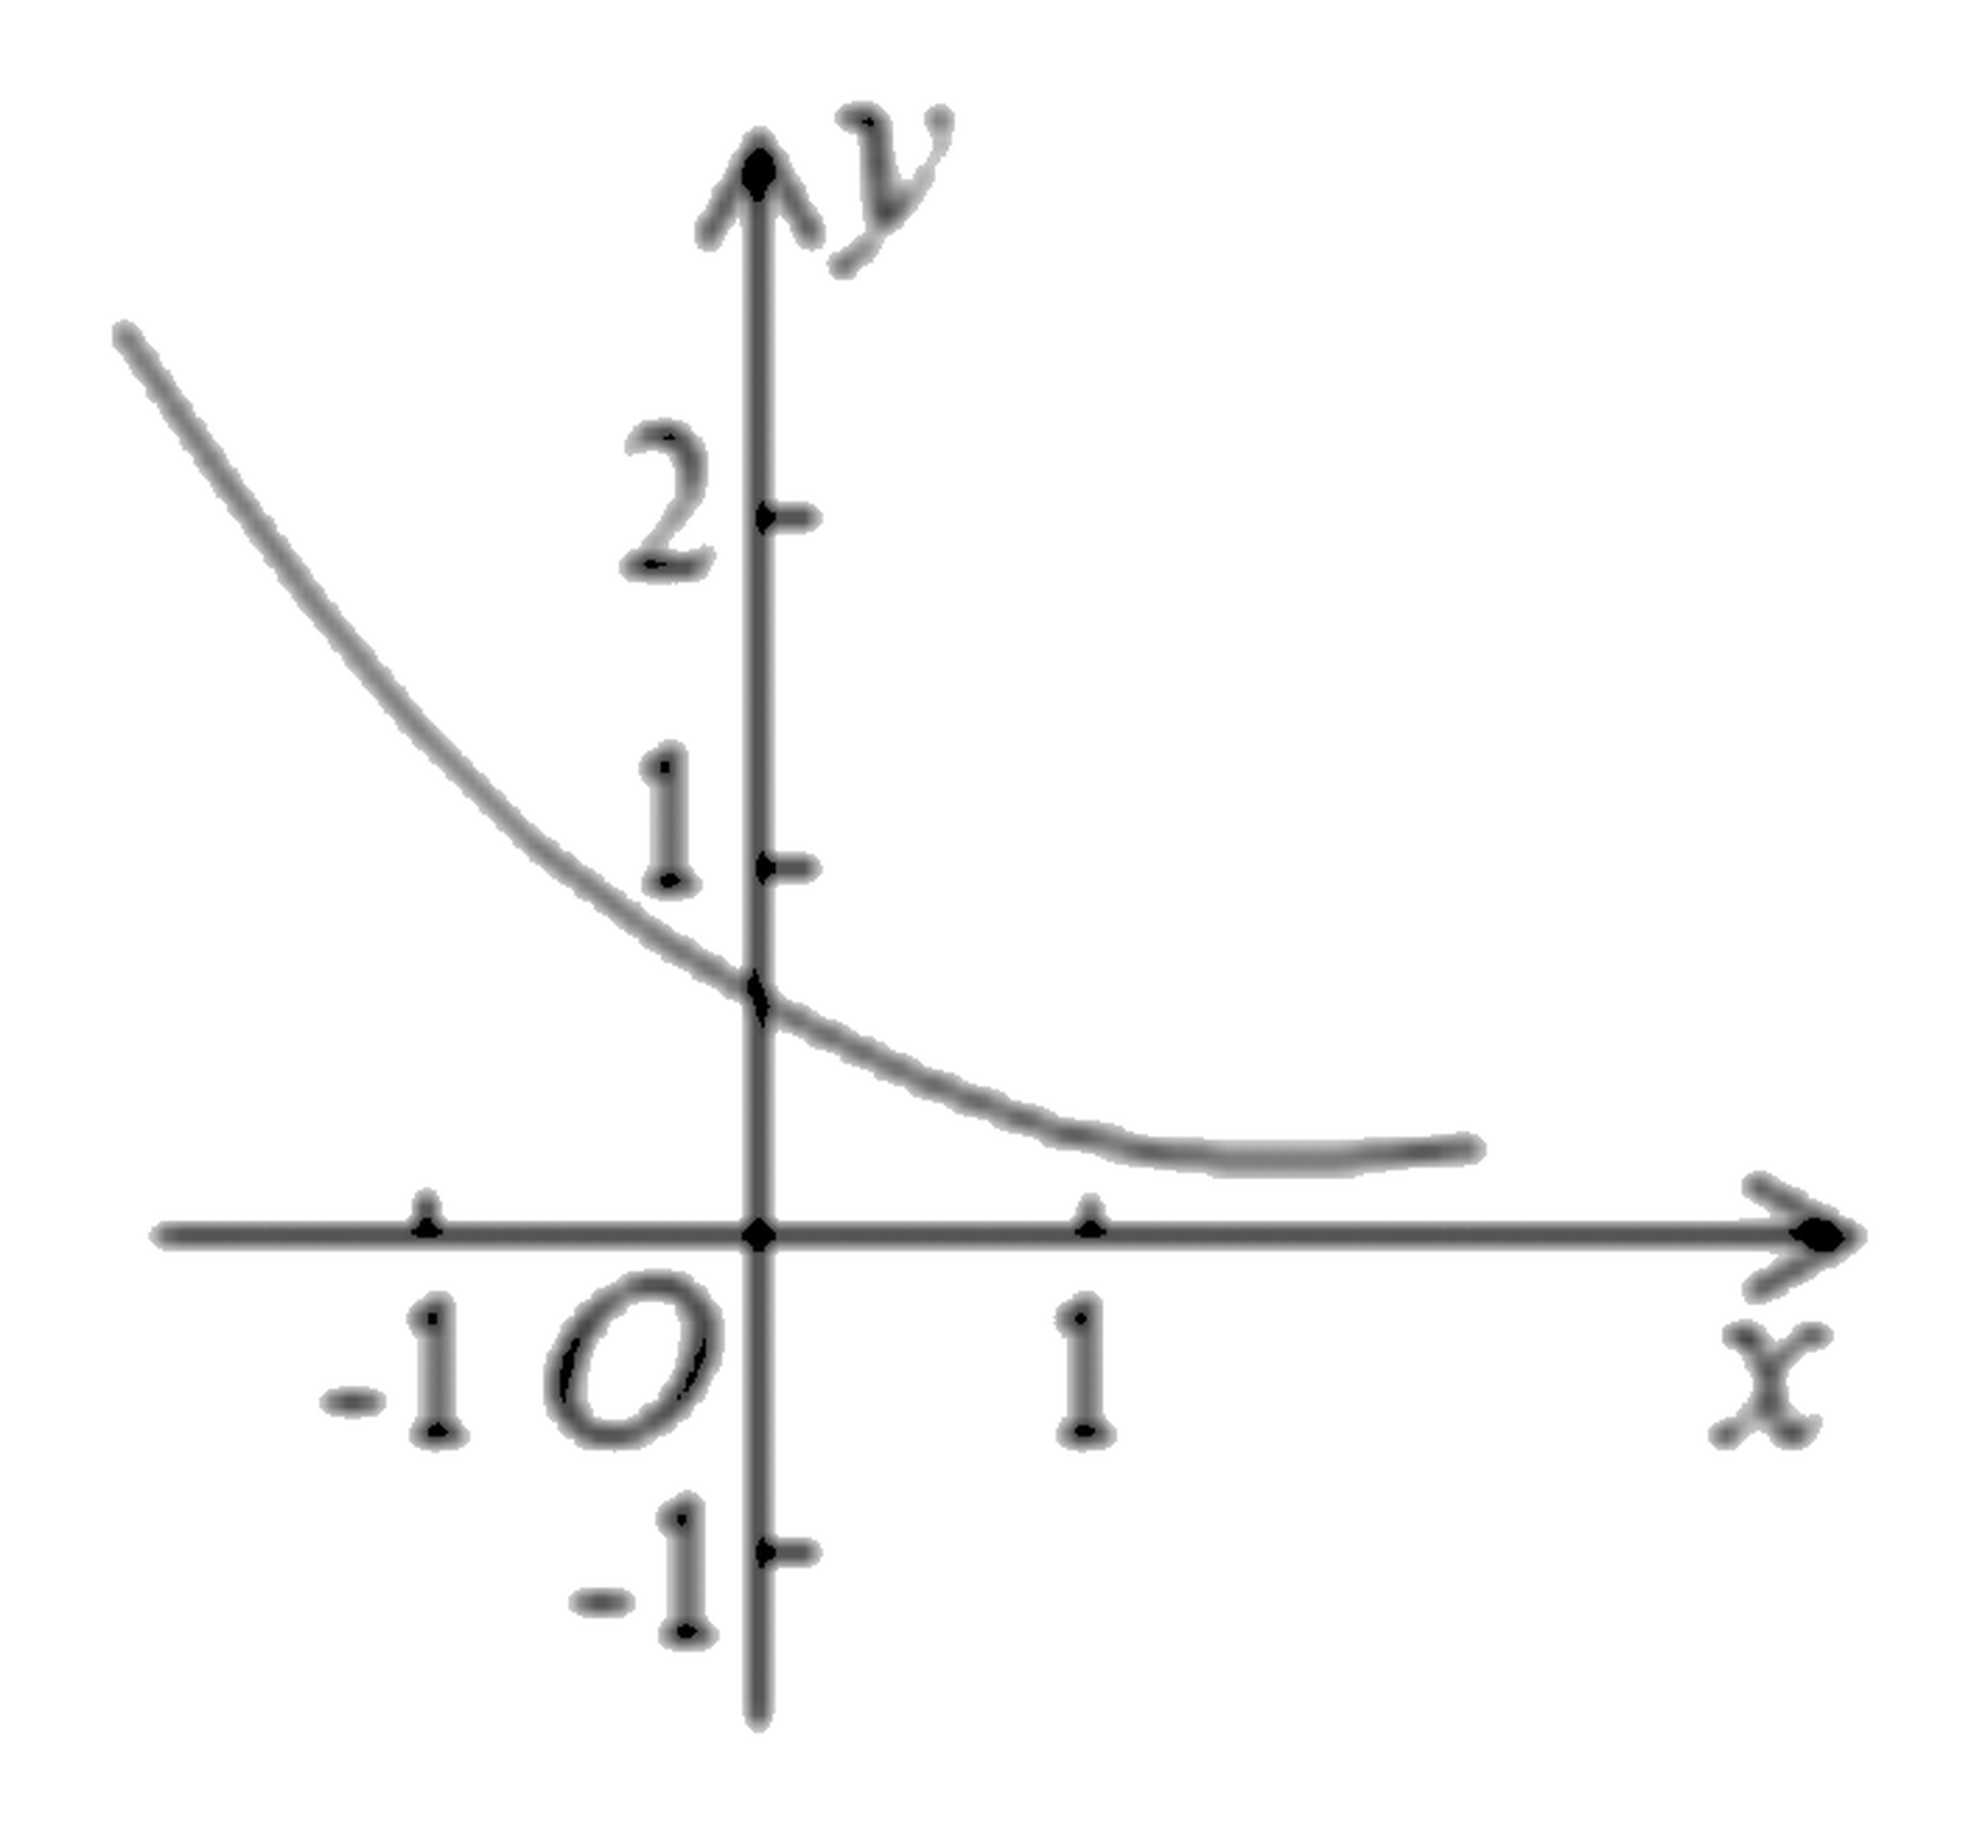
\includegraphics[width=0.30\textwidth]{figures/gao147_q15.png}
\end{center}

\ifanswer
\solbegin
\step{由图象从左到右下降得 $0<a<1$；}
\step{由图象与 $y$ 轴的交点得 $0<a^{-b}<1$，故 $b<0$；}
\step{故 $0<a<1$，$b<0$；故选 $D$.}
\solend
\fi

% === Q16 ===：位数新定义题（无弯引号，放大 04 页 z/q16_stem.png 确认）；四选项横排一行；解析 3 个印刷行
\item 数学运算是指在明晰运算对象的基础上，依据运算法则解决数学问题的素养. 因为运算，数的威力无限；没有运算，数就只是一个符号，对数运算与指数运算是两类重要的运算，对数的运算性质降低了运算的级别，简化了运算，在数学发展史上是伟大的成就. 而位数是指一个自然数有效位的个数，例如：$2^{10}=1024$，所以 $2^{10}$ 的位数为 4. 请你运用所学过的对数运算的知识，估计 $2025^{2026}$ 的位数是\mbox{（\quad）}

\keepwithprev
A. 6697\qquad B. 6698\qquad C. 6699\qquad D. 6700

\ifanswer
\solbegin
\step{设 $2025^{2026}=t$，所以 $\lg t=2026\lg2025$，}
\step{因为 $\lg2025\approx3.3064$，所以 $\lg t\approx6698.8$，}
\step{所以 $t\approx10^{6698.8}\in(10^{6698},10^{6699})$，所以 $2025^{2026}$ 的位数为 6699. 故选 $C$.}
\solend
\fi

\end{enumerate}

\bigsec{三、解答题}

\begin{enumerate}
\setcounter{enumi}{16}

% === Q17 ===：题干＋解析均在 04 页；集合描述竖线 \mid、描述内半角逗号照录；
% 空集 \varnothing、子集 \subseteq（放大 04 页 z/subset_04_q17b.png 确认带下划线）、数集 \R；
% 解析 5 个印刷行，首行末"所以 A=(-∞,-2)∪(3,+∞)"原卷无标点，照录不补
\item 已知集合 $A=\left\{x\mid \dfrac{x+2}{x-3}>0,x\in\R\right\}$，$B=\{x\mid \lvert x-2a\rvert\leqslant2,x\in\R\}$.

(1) 若 $a=1$，求 $A\cap B$；

(2) 若 $A\cap B=\varnothing$，求实数 $a$ 的取值范围.

\ifanswer
\solbegin
\step{由 $\dfrac{x+2}{x-3}>0$，得 $x<-2$ 或 $x>3$，所以 $A=(-\infty,-2)\cup(3,+\infty)$}
\step{(1) 当 $a=1$ 时，$B=\{x\mid \lvert x-2\rvert\leqslant2\}=[0,4]$，于是 $A\cap B=(3,4]$；}
\step{(2) $B=[2a-2,2a+2]$，}
\step{则 $A\cap B=\varnothing\Leftrightarrow[2a-2,2a+2]\subseteq[-2,3]\Leftrightarrow\begin{cases}2a-2\geqslant-2\\2a+2\leqslant3\end{cases}\Leftrightarrow0\leqslant a\leqslant\dfrac{1}{2}$，}
\step{所以实数 $a$ 的取值范围为 $\left[0,\dfrac{1}{2}\right]$.}
\solend
\fi

% === Q18 ===：氟化物／臭氧应用题；"氟化物""（如冰箱等）"全角夹注照录（放大 05 页 z/q18_line1.png 确认）；
% 关系式 $Q=Q_0e^{-0.0025t}$ 原卷独立一行，按一段照录；解析 6 个印刷行
\item 有些家用电器（如冰箱等）使用了氟化物，氟化物的释放破坏了大气上层的臭氧层，使臭氧含量 $Q$ 呈指数函数型变化，在氟化物排放量维持某种水平时，具有关系式

$Q=Q_0e^{-0.0025t}$，其中 $Q_0$ 是臭氧的初始量.

(1) 随时间 $t$ 的增加，臭氧的含量是增加还是减少？

(2) 试估计多少年以后将会有一半的臭氧消失.（用计算器计算）

\ifanswer
\solbegin
\step{(1) 对于函数 $Q=Q_0e^{-0.0025t}$，显然 $Q>0$，}
\step{任取 $t_1$、$t_2\in(0,+\infty)$，且 $t_1<t_2$，则 $t_2-t_1>0$，}
\step{所以 $\dfrac{Q_1}{Q_2}=\dfrac{Q_0e^{-0.0025t_1}}{Q_0e^{-0.0025t_2}}=e^{-0.0025(t_1-t_2)}=e^{0.0025(t_2-t_1)}>e^0=1$，所以 $Q_1>Q_2$，}
\step{故随着时间 $t$ 的增加，臭氧的含量是减少的；}
\step{(2) 令 $\dfrac{Q}{Q_0}=\dfrac{1}{2}$，即 $\dfrac{Q_0e^{-0.0025t}}{Q_0}=e^{-0.0025t}=\dfrac{1}{2}$，得 $-0.0025t=\ln\dfrac{1}{2}\approx-0.6931$，}
\step{解得 $t\approx277$，故估计 277 年以后将会有一半的臭氧消失.}
\solend
\fi

% === Q19 ===：题干用"图像"、解析两处用"图象"逐处照录不统一（05 页）；数集 \Z；
% 题干＋解析前 4 行在 05 页、解析后 3 行在 06 页；解析共 7 个印刷行
\item 已知幂函数 $f(x)=x^{-m^2+4m}(m\in\Z)$ 的图像关于 $y$ 轴对称，且在区间 $(0,+\infty)$ 上是严格增函数.

(1) 求 $m$ 的值；

(2) 求满足不等式 $(2a+1)^m<(a+1)^m$ 的实数 $a$ 的取值范围.

\ifanswer
\solbegin
\step{(1) 由题意得 $-m^2+4m>0$，解得 $0<m<4$，}
\step{因为 $m\in\Z$，所以 $m=1$ 或 $m=2$ 或 $m=3$.}
\step{当 $m=1$ 或 $m=3$ 时，$f(x)=x^3$，图象关于原点对称，不合题意；}
\step{当 $m=2$ 时，$f(x)=x^4$，图象关于 $y$ 轴对称，符合题意，所以 $m=2$.}
\step{(2) 代入 $m=2$，不等式为 $(2a+1)^2<(a+1)^2$，}
\step{得 $(2a+1)^2-(a+1)^2=a(3a+2)<0$，因此 $-\dfrac{2}{3}<a<0$，}
\step{所求范围为 $\left(-\dfrac{2}{3},0\right)$.}
\solend
\fi

% === Q20 ===：指数函数题，题干用"图像"；(3) 长求和式（分数 1/2026、1011/2026、2011/2026、
% 15/2026、1015/2026、2025/2026 放大 06 页 z/q20_sum_06a.png 确认）；题干在 06 页、
% 解析前 6 行在 06 页下半、后 6 行在 07 页上半；解析共 12 个印刷行
\item 已知指数函数 $y=a^x$（$a>0,a\ne1$）的图像经过点 $(1,4)$.

(1) 求实数 $a$ 的值；

(2) 若 $f(x)=(a^x)^2-2\cdot a^x-8$，当 $x\in\R$ 时，不等式 $f(x)>m\cdot4^x-12$ 恒成立，求 $m$ 的取值范围；

(3) 记 $g(x)=\dfrac{1}{a^x+2}$，求证：$g(x)+g(1-x)$ 为定值，并求 $g(0)+g\left(\dfrac{1}{2026}\right)+g\left(\dfrac{1011}{2026}\right)+g\left(\dfrac{2011}{2026}\right)+g\left(\dfrac{1}{2}\right)+g\left(\dfrac{15}{2026}\right)+g\left(\dfrac{1015}{2026}\right)+g\left(\dfrac{2025}{2026}\right)+g(1)$ 的值.

\ifanswer
\solbegin
\step{(1) 将 $(1,4)$ 代入 $y=a^x$，得 $a^1=4$，即 $a=4$.}
\step{(2) 令 $t=4^x$，当 $x\in\R$ 时，$t$ 取遍所有正实数.}
\step{原不等式等价于 $t^2-2t-8>mt-12\Leftrightarrow m<t+\dfrac{4}{t}-2$，}
\step{由基本不等式，$t+\dfrac{4}{t}-2\geqslant2\sqrt{t\cdot\dfrac{4}{t}}-2=2$，}
\step{当且仅当 $t=\dfrac{4}{t}$，即 $t=2$ 时取等号，}
\step{因此原不等式恒成立的充要条件为 $m<2$，即 $m\in(-\infty,2)$.}
\step{(3) 对任意 $x\in\R$，令 $t=4^x>0$，则 $4^{1-x}=\dfrac{4}{t}$，}
\step{从而 $g(x)+g(1-x)=\dfrac{1}{t+2}+\dfrac{1}{\dfrac{4}{t}+2}=\dfrac{1}{t+2}+\dfrac{t}{2(t+2)}=\dfrac{1}{2}$，}
\step{因此 $g(x)+g(1-x)$ 为定值 $\dfrac{1}{2}$.}
\step{原式中，0 与 1、$\dfrac{1}{2026}$ 与 $\dfrac{2025}{2026}$、$\dfrac{1011}{2026}$ 与 $\dfrac{1015}{2026}$、$\dfrac{2011}{2026}$ 与 $\dfrac{15}{2026}$}
\step{分别配对，每对函数值之和均为 $\dfrac{1}{2}$，且 $g\left(\dfrac{1}{2}\right)=\dfrac{1}{4^{\frac12}+2}=\dfrac{1}{4}$，}
\step{所以所求和为 $4\cdot\dfrac{1}{2}+\dfrac{1}{4}=\dfrac{9}{4}$.}
\solend
\fi

% === Q21 ===：不动点新定义题；题干在 07 页、解析续 08／09 页，共 20 个印刷行；
% 判别式两形混用：08 页 (2) cases 内等腰偏高 \Delta、09 页 (3) 扁等边 \triangle，逐处照录不统一
% （放大 /tmp/gao147/z/delta_vs_triangle.png 并排确认）；数集 \R；\forall 照录；
% 第 6—8 行是原卷一个长算式折成的三个印刷行，按印刷行分三条 \step、不并折行
\item 对于二次函数 $y=mx^2+nx+t(m\ne0)$，若存在 $x_0\in\R$，使得 $mx_0^2+nx_0+t=x_0$ 成立，则称 $x_0$ 为二次函数 $y=mx^2+nx+t(m\ne0)$ 的不动点.

(1) 求二次函数 $y=x^2-x-3$ 的不动点；

(2) 若二次函数 $y=2x^2-(3+a)x+a-1$ 有两个不相等的不动点 $x_1$、$x_2$，且 $x_1$、$x_2>0$，求 $\dfrac{x_1}{x_2}+\dfrac{x_2}{x_1}$ 的最小值；

(3) 若对任意实数 $b$，二次函数 $y=ax^2+(b+1)x+(b-1)(a\ne0)$ 恒有不动点，求 $a$ 的取值范围.

\ifanswer
\solbegin
\step{(1) 令 $x^2-x-3=x$，即 $x^2-2x-3=0$，即 $(x-3)(x+1)=0$，}
\step{解得 $x_1=-1$，$x_2=3$，所以不动点为 $-1$ 和 $3$.}
\step{(2) 由题意，$2x^2-(3+a)x+a-1=x$ 有两个不相等的正实数根，}
\step{即方程 $2x^2-(4+a)x+a-1=0$ 有两个不相等的正实数根，}
\step{所以 $\begin{cases}\Delta=(4+a)^2-8(a-1)>0\\x_1+x_2=\dfrac{4+a}{2}>0\\x_1\cdot x_2=\dfrac{a-1}{2}>0\end{cases}$，解得 $a>1$，}% 判别式原卷印等腰偏高粗三角 $\Delta$（放大 08 页 z/delta_08_q21cases.png）
\step{所以 $\dfrac{x_1}{x_2}+\dfrac{x_2}{x_1}=\dfrac{x_1^2+x_2^2}{x_1\cdot x_2}=\dfrac{(x_1+x_2)^2-2x_1\cdot x_2}{x_1\cdot x_2}=\dfrac{(x_1+x_2)^2}{x_1\cdot x_2}-2$}
\step{$=\dfrac{\left(\dfrac{4+a}{2}\right)^2}{\dfrac{a-1}{2}}-2=\dfrac{\dfrac{(a+4)^2}{4}}{\dfrac{a-1}{2}}-2=\dfrac{(a-1+5)^2}{2(a-1)}-2$}
\step{$=\dfrac{(a-1)^2+10(a-1)+25}{2(a-1)}-2=\dfrac{a-1}{2}+\dfrac{25}{2(a-1)}+3$.}
\step{因为 $a>1$，所以 $a-1>0$，}
\step{所以 $\dfrac{a-1}{2}+\dfrac{25}{2(a-1)}+3\geqslant2\sqrt{\dfrac{a-1}{2}\cdot\dfrac{25}{2(a-1)}}+3=8$，}
\step{当且仅当 $\dfrac{a-1}{2}=\dfrac{25}{2(a-1)}$，即 $a=6$ 时等号成立，}
\step{所以 $\dfrac{x_1}{x_2}+\dfrac{x_2}{x_1}$ 的最小值为 $8$.}
\step{(3) 设 $f(x)=ax^2+(b+1)x+b-1$，}
\step{则方程 $f(x)=x$，可化为 $ax^2+(b+1)x+b-1=x$，}
\step{即 $ax^2+bx+b-1=0$，}
\step{由题意得一元二次方程 $ax^2+bx+b-1=0$ 有解，又 $a\ne0$，}
\step{所以方程 $ax^2+bx+b-1=0$ 的判别式 $\triangle=b^2-4a(b-1)\geqslant0$，}% 判别式原卷印扁等边细线三角 $\triangle$（放大 09 页 z/triangle_09_q21.png），与 (2) 高 $\Delta$ 混用、照录不统一
\step{即 $b^2-4ab+4a\geqslant0$，则该不等式对 $\forall b\in\R$ 恒成立，}
\step{则 $(4a)^2-4\times4a\leqslant0$，且 $a\ne0$，解得 $0<a\leqslant1$，}
\step{所以实数 $a$ 的取值范围是 $(0,1]$.}
\solend
\fi

\end{enumerate}

\end{document}
"
% 紧凑版：xelatex "\def\iscompact{1}% 高一147_华师大三附中_期中.tex
%   —— 高一上数学"2026-2027 年华师大三附中高一上期中"（试卷版/答案版/紧凑版）
% 试卷版：xelatex 高一147_华师大三附中_期中.tex
% 答案版：xelatex "\def\isanswer{1}% 高一147_华师大三附中_期中.tex
%   —— 高一上数学"2026-2027 年华师大三附中高一上期中"（试卷版/答案版/紧凑版）
% 试卷版：xelatex 高一147_华师大三附中_期中.tex
% 答案版：xelatex "\def\isanswer{1}\input{高一147_华师大三附中_期中.tex}"
% 紧凑版：xelatex "\def\iscompact{1}\input{高一147_华师大三附中_期中.tex}"
%
% ① 原始材料：微信公众号"魔都数学加油站"文章，连载"27学年高一147"，原文标题
% "27学年高一147——2026-2027年上海市华师大三附中高一上期中"；
% 原文链接：https://mp.weixin.qq.com/s/X_gPW1JWoTAl2Bky_xEEGw 。
% 正文为 9 张 PNG 页（01/06/08/09 为 2560×3620，02/03/04/05/07 为 4762×6735，
% 同一篇各页分辨率混排，逐页按各自分辨率裁图核对，别按预览比例换算裁框）。
% 体例：混合体例讲评版——19 题中 Q4/Q5/Q7/Q9 只印【答案】、无【解析】，其余 15 题印
% 【解析】（逐题核实，见 ② ②）。题目、答案、解析均据原图转录；卷面粉红色水印
% "魔都数学加油站"及公众号页脚未录入。
% 全卷插图清单（逐页通读 9 页确认）：仅 1 处题目配图——
%   · Q15 递减指数函数小坐标系（03 页右侧：坐标轴、y 轴刻度 2/1/-1、x 轴刻度 -1/1、
%     原点 O、x/y 轴标），为"图像如图所示"的题目配图（选择题选项旁），三版都出；
%     裁自 03 页去粉色水印、去色、4× LANCZOS 放大存 figures/gao147_q15.png；
%   其余 8 页逐页确认无其它题目配图、无【解析】内配图、无表格，
%   亦无"题干写如图而源码漏图"一处；Q12/Q17/Q21 的 cases 块为数学块（非图）。
%
% 卷首标题：原卷印作"2026-2027 年华师大三附中高一上期中"，年份区间按全稿惯例排 en dash；
% 原卷卷面未印副标题，本稿按同期中卷（高一140／141／143／144／145／146）知识模块口径
% 补出"集合与常用逻辑用语、不等式、函数"。
%
% 题号体例（逐页核实定稿）：本卷共 19 题——一、填空题 3—12（10 题）、
% 二、选择题 13—16（4 题）、三、解答题 17—21（5 题）。
% 三节分别 \setcounter{enumi}{2}／{12}／{16}。原卷从第 3 题起、无第 1、2 题，
% 本稿保留原题号；全卷无附加题节（Q21 解析末行"所以实数 a 的取值范围是 (0,1]."
% 为全卷收尾，09 页下半仅水印、无正文）。
%
% ② 与原卷的排版差异：
%   ① 原文从第 3 题起，本稿保留原题号；共 19 题三节；
%   ② 混合体例：原卷 Q4/Q5/Q7/Q9 只印【答案】、无【解析】（分别为 a≤0、(-1,2)、
%      真、(-∞,1)），按 高一140 第 5 题／高一145 Q3 成例提 \ans{}、不补造解析；
%      其余 15 题印【解析】，用 \solbegin…\solend，选择题答案在解析末句"故选 X"
%      （Q13 选 B、Q14 选 B、Q15 选 D、Q16 选 C，逐个放大原图核实）、题干括号
%      \mbox{（\quad）} 留空、不另提 \ans{}；填空／解答答案落在解析里；
%      答案版【答案】/【解析】标记数 = 19（4 个 \ans ＋ 15 个 \solbegin）= 全卷题数；
%   ③ 原卷卷面未印副标题，本稿按知识模块口径补出；
%   ④ 原卷填空横线按全稿惯例排 \blankline[4.4em]；选择题括号排 \mbox{（\quad）}、
%      选项段前按惯例加 \keepwithprev；Q14／Q15 四选项为 2×2 两印刷行（A/B 一行、
%      C/D 一行），用空行分段照录（非一行 \qquad、亦非竖排四行）；解答题不留作答区、
%      不加 \anspace（原卷为讲评版，与 129／131／132／133／136／140／141／143／144／145／146 同）；
%   ⑤ 数集：Q4"A∪B=R"、Q13"f(x)=x^3 在 R 上严格增"、Q17"x∈R"两处、
%      Q20"x∈R"两处、Q21"x_0∈R""∀b∈R"原卷印斜体或黑板粗体 R，按全稿惯例统一改 \R；
%      Q19"m∈Z"改 \Z；本卷未出现 N（\N^* 无对应处）。绝对值排 \lvert…\rvert，
%      集合描述竖线排 \mid；不等号按全稿惯例排 \leqslant／\geqslant（原卷印 \le／\ge 形，
%      【答案】a≤0 亦排 \leqslant）；空集 \varnothing（Q17 两处）；
%      子集 \subseteq（Q17 带下划线，放大 04 页确认）；本卷未出现 \subset／\subsetneq，
%      亦未出现补集上划线 \overline{}；\left…\right 不得拆到不同 $…$ 组；
%   ⑥ 子题标号 (1)(2)(3) 半角括号照录；cases 块整体算一个印刷行（Q3、Q12 一行内
%      两个 cases、Q17、Q21(2)）；本卷解析内无圈数字①②③（无 \text{①} 需求）；
%      数学式内 CJK 用 \text{}（本卷未见）；
%   ⑦ 题干中的中文弯引号按原卷照录：Q7 命题"若 A∪B=B，则 A∩B=A"与
%      (填 " 真 " 或 " 假 ")、Q10 (填 ">" "<" "≤" "或≥")，含引号内空格；
%      注释内一律 ASCII 引号；Q16 位数新定义题逐字放大确认无弯引号
%      （交办提示的"Q16 新定义题"举例未在本卷出现），未补造引号；
%   ⑧ 半角逗号在数学组之间是全稿惯例、非笔误（Q4"$A=(-\infty,0],B=[a,+\infty)$"、
%      Q5"$(a>0,a\ne1)$"、Q17 集合描述内"$>0,x\in R$""$\leqslant2,x\in R$"、
%      Q20 题干"$(a>0,a\ne1)$"、Q21"$y=mx^2+nx+t(m\ne0)$"等），逐处照录别改全角；
%      行末西文句点照录为 ASCII `.`；行中全角逗号／顿号照录；
%      Q7／Q10"(填…)"为半角括号、Q18"（如冰箱等）"为全角括号，逐处照录不统一；
%   ⑨ "图像／图象"逐处照录不统一：题干 5 处用"图像"（Q5"图像恒过定点"、
%      Q9"图像位于直线 y=x 的下方"、Q15"的图像如图所示"、Q19"的图像关于 y 轴对称"、
%      Q20"的图像经过点"），解析 4 处用"图象"（Q15"由图象从左到右下降"
%      "由图象与 y 轴的交点"、Q19"图象关于原点对称""图象关于 y 轴对称"），逐处核、不统一；
%   ⑩ 判别式 Δ/△ 混用是照录项：Q21(2) 解析 cases 块"Δ=(4+a)²−8(a−1)>0"
%      印等腰偏高粗三角 \Delta，Q21(3) 解析"判别式△=b²−4a(b−1)≥0"
%      印扁等边细线三角 \triangle，逐处放大判断、照录不得统一
%      （参照 高一142／144／145 头注④口径，详见 ④）；
%   ⑪ 一条 \step = 原卷解析的一个印刷行，cases 块整体算一个印刷行；别把原卷折行
%      并起来、别把一行拆多条。Q10 七行（跨 01→02 页）、Q12 七行（含一行两 cases）、
%      Q20 十二行（含"原式中…2011/2026 与 15/2026／分别配对…"折行两行）、
%      Q21 二十行（含第 6—8 行一个长算式折成三印刷行、含 cases）均按印刷行逐条断，
%      不丢行；
%   ⑫ 配图：逐页通读 9 页确认全卷仅 Q15 一处题目配图（见 ①），三版都出、
%      \includegraphics[width=0.30\textwidth]；图块较小，未加 \needvspace 大图块守卫
%      （仅 \bigsec 自带 \needvspace{3\baselineskip}）；三版切页审计均"合计异常：无"；
%   ⑬ 跨页续印按题合并：Q3—Q9 在 01 页（Q10 题干在 01 页末、解析首行亦在 01 页末）；
%      Q10 解析续 02 页 6 行、Q11 在 02 页、Q12 题干＋解析前 4 行在 02 页
%      （解析续 03 页 3 行）；"二、选择题"标题与 Q13、Q14、Q15 题干＋解析前 2 行在 03 页
%      （Q15 配图在 03 页右侧）；Q15 解析末行与 Q16、"三、解答题"标题、Q17 在 04 页；
%      Q18 在 05 页、Q19 题干＋解析前 4 行在 05 页（解析续 06 页 3 行）；
%      Q20 题干＋解析前 6 行在 06 页（解析续 07 页 6 行）、Q21 题干＋解析前 3 行在 07 页；
%      Q21 解析续 08 页 13 行、续 09 页 4 行（09 页下半仅水印、无正文）。
%      本稿按题连排，不丢行、不并折行；
%   ⑭ 原卷解析内无红色"法一／法二"之类小标题，故本卷无 \stepm；
%      水印"魔都数学加油站"红色不录入。
%
% ③ 行数复核：一条 \step／\stepm = 原卷解析的一个印刷行，cases 块作一个印刷行计。
%   逐题数（主会话逐页核对定稿）：Q3：1；Q4：0（只印【答案】、提 \ans{}，不计入 \step 账）；
%   Q5：0；Q6：1；Q7：0；Q8：2；Q9：0；Q10：7；Q11：4；Q12：7；Q13：6；Q14：4；
%   Q15：3；Q16：3；Q17：5；Q18：6；Q19：7；Q20：12；Q21：20。
%   合计 88 条 \step（本卷无 \stepm：解析内无红色"法一／法二"类小标题），
%   与原卷逐题印刷行相等。全卷 15 题设 \solbegin…\solend ＋ 4 题一处 \ans{}，
%   答案版【答案】/【解析】标记数 = 19 = 全卷题数。
%
% ④ 判别式／子集符号结论（逐处放大原图照录、不得统一，主会话像素级复核）：
%   判别式全卷 2 处、两形混用逐处照录不统一（参照 高一142／144 头注④口径）：
%     · Q21(2) 解析 cases 块"Δ=(4+a)²−8(a−1)>0" 原卷印等腰偏高粗三角
%       （高>宽、粗笔画），照录 \Delta（放大 08 页 /tmp/gao147/z/delta_08_q21cases.png
%       与 z/delta_vs_triangle.png 左图确认）；
%     · Q21(3) 解析"判别式△=b²−4a(b−1)≥0" 原卷印扁等边细线三角
%       （宽≈高、细线），照录 \triangle（放大 09 页 /tmp/gao147/z/triangle_09_q21.png
%       与 z/delta_vs_triangle.png 右图并排确认）。
%   子集／补集：Q17 解析"[2a−2,2a+2]⊆[−2,3]" 原卷印带下划线 ⊆，照录 \subseteq
%     （放大 04 页 /tmp/gao147/z/subset_04_q17b.png 确认）；Q17"A∩B=∅"空集 \varnothing；
%     集合描述竖线 \mid（Q10 M、Q12 解集、Q17 A/B）；并集 \cup（Q4、Q17）、
%     交集 \cap（Q7、Q17）、不属于 \notin（Q10）；数集 \R／\Z 归一见 ② ⑤。
%   本卷未出现 \subset／\subsetneq，未出现补集上划线 \overline{}。
%
% ⑤ 存疑照录（放大原图确认，照录未改、正文对应处另有 % 注）：
%   1. Q4/Q5/Q7/Q9 只印【答案】、无【解析】，按成例提 \ans{}、不补造解析
%      （混合体例逐题核实，见 ② ②）。
%   2. Q21(2) 判别式高 \Delta 与 Q21(3) 判别式扁 \triangle 两形混用，
%      逐处照录不统一（见 ④）。
%   3. "图像／图象"题干 5 处"图像"、解析 4 处"图象"，逐处照录不统一（见 ② ⑨）。
%   4. Q7／Q10"(填…)"半角括号与 Q18"（如冰箱等）"全角括号，逐处照录不统一。
%   5. Q16 位数新定义题逐字放大确认无弯引号（交办提示的"Q16 新定义题"举例
%      未在本卷出现），未补造引号；全卷弯引号仅 Q7、Q10 两处。
%   6. Q17 解析首行末"所以 A=(-∞,-2)∪(3,+∞)"、Q20(3) 解析"…2011/2026 与 15/2026"
%      行末原卷均无标点，照录未补；Q21(2) 第 6—8 行一个长算式折成三印刷行，
%      按印刷行分三条 \step、不并折行。
%   全卷除此 6 类外未发现其它笔误／自相矛盾处。
%
% ⑥ 跨页续印按题合并说明：见 ② ⑬。
%
\documentclass[a4paper,11pt]{article}
\usepackage{common}

\begin{document}

\examtitlest[3]{2026--2027 年华师大三附中高一上期中}{集合与常用逻辑用语、不等式、函数}

\bigsec{一、填空题}

\begin{enumerate}
\setcounter{enumi}{2}

% === Q3 ===：印【解析】，1 个印刷行（cases 块整体算一行）
\item 函数 $y=(a^2-5a+7)a^x+6-2a$ 是指数函数，则 $a$ 的值为\blankline[4.4em].

\ifanswer
\solbegin
\step{由题意得 $\begin{cases}a^2-5a+7=1\\6-2a=0\end{cases}$，解得 $a=3$.}
\solend
\fi

% === Q4 ===：原卷只印【答案】、无【解析】，按 高一140 第 5 题／高一145 Q3 成例提 \ans{}、不补造解析；
% 题干数学组内半角逗号 $A=(-\infty,0],B=[a,+\infty)$ 照录（放大 01 页 z/q4_stem.png 确认）
\item 已知 $A=(-\infty,0],B=[a,+\infty)$，且 $A\cup B=\R$，则实数 $a$ 的取值范围为\blankline[4.4em].

\ifanswer
\ans{$a\leqslant0$}
\fi

% === Q5 ===：只印【答案】；题干"图像"照录（放大 01 页 z/q5_stem.png 确认）；
% 数学组内半角逗号 $(a>0,a\ne1)$ 照录
\item 函数 $y=a^{x+1}+1(a>0,a\ne1)$ 的图像恒过定点\blankline[4.4em].

\ifanswer
\ans{$(-1,2)$}
\fi

% === Q6 ===：印【解析】，1 个印刷行
\item 已知方程 $x^2+2x-4=0$ 的两个根为 $x_1$、$x_2$，则 $x_1^2+x_2^2$ 的值为\blankline[4.4em].

\ifanswer
\solbegin
\step{$x_1^2+x_2^2=(x_1+x_2)^2-2x_1x_2=4+8=12$.}
\solend
\fi

% === Q7 ===：只印【答案】；中文弯引号"若 A∪B=B，则 A∩B=A"与(填 " 真 " 或 " 假 ")内的空格照录
% （放大 01 页 z/q7_quotes_7x.png、z/q7_tail.png 确认，括号为半角）
\item 命题 “若 $A\cup B=B$，则 $A\cap B=A$” 为\blankline[4.4em]命题(填 “ 真 ” 或 “ 假 ”).

\ifanswer
\ans{真}
\fi

% === Q8 ===：印【解析】，2 个印刷行；不等号按全稿惯例 \geqslant／\leqslant
\item 已知正实数 $a$、$b$ 满足 $a+4b=1$，则 $ab$ 的最大值为\blankline[4.4em].

\ifanswer
\solbegin
\step{$a+4b\geqslant2\sqrt{a\cdot4b}\Rightarrow ab\leqslant\dfrac{1}{16}$，当且仅当 $a=4b=\dfrac{1}{2}$ 时取等号，}
\step{则 $ab$ 的最大值为 $\dfrac{1}{16}$.}
\solend
\fi

% === Q9 ===：只印【答案】；题干"图像"照录（放大 01 页 hi_01_2 确认）
\item 若幂函数 $y=x^s$ 在 $x>1$ 时的图像位于直线 $y=x$ 的下方，则 $s$ 的取值范围是\blankline[4.4em].

\ifanswer
\ans{$(-\infty,1)$}
\fi

% === Q10 ===：印【解析】，共 7 个印刷行（题在 01 页末起 1 行、续 02 页 6 行）；
% 题干跨两印刷行"则 |ab|+1 ____ |a|+|b|（填…）"按一句连排；(填…)为半角括号、引号内空格照录
\item 已知不等式 $\lvert2x+1\rvert+\lvert2x-1\rvert<4$ 的解集为 $M$. 设实数 $a\in M$，$b\notin M$，则 $\lvert ab\rvert+1$\blankline[4.4em] $\lvert a\rvert+\lvert b\rvert$(填 “$>$”，“$<$”，“$\leqslant$” “或$\geqslant$”).

\ifanswer
\solbegin
\step{当 $x<-\dfrac{1}{2}$ 时，不等式化为 $-2x-1+1-2x<4$，即 $x>-1$，所以 $-1<x<-\dfrac{1}{2}$；}
\step{当 $-\dfrac{1}{2}\leqslant x\leqslant\dfrac{1}{2}$ 时，不等式化为 $2x+1-2x+1<4$，即 $2<4$，所以 $-\dfrac{1}{2}\leqslant x\leqslant\dfrac{1}{2}$；}
\step{当 $x>\dfrac{1}{2}$ 时，不等式化为 $2x+1+2x-1<4$，即 $x<1$，所以 $\dfrac{1}{2}<x<1$；}
\step{综上，$M=\{x\mid -1<x<1\}$.}
\step{因为 $a\in M$，$b\notin M$，所以 $\lvert a\rvert<1$，$\lvert b\rvert\geqslant1$.}
\step{而 $\lvert ab\rvert+1-(\lvert a\rvert+\lvert b\rvert)=\lvert ab\rvert+1-\lvert a\rvert-\lvert b\rvert=(\lvert a\rvert-1)(\lvert b\rvert-1)$，}
\step{所以 $\lvert ab\rvert+1\leqslant\lvert a\rvert+\lvert b\rvert$.}
\solend
\fi

% === Q11 ===：印【解析】，4 个印刷行（02 页）
\item 已知 $m>1$，$n>1$，$\lg m=\log_n100$，则 $mn$ 的最小值为\blankline[4.4em].

\ifanswer
\solbegin
\step{由 $m>1$，$n>1$，得 $\lg m>0$，$\lg n>0$，}
\step{因为 $\lg m=\log_n100=\dfrac{\lg100}{\lg n}=\dfrac{2}{\lg n}$，所以 $\lg m\cdot\lg n=2$，}
\step{所以 $\lg(mn)=\lg m+\lg n\geqslant2\sqrt{\lg m\cdot\lg n}=2\sqrt2$，}
\step{当且仅当 $m=n=10^{\sqrt2}$ 时取等号，则 $mn\geqslant10^{2\sqrt2}$，即 $mn$ 的最小值为 $10^{2\sqrt2}$.}
\solend
\fi

% === Q12 ===：印【解析】，共 7 个印刷行（02 页 4 行、03 页 3 行）；
% 第 3 行"则 [cases]，得 [cases]，"两个 cases 块同属一个印刷行，整体作一条 \step（照 高一146 Q11 成例）
\item 已知关于 $x$ 的不等式 $ax^2+bx+c\leqslant1$ 的解集为 $\{x\mid -1\leqslant x\leqslant3\}$. 若关于 $x$ 的不等式 $ax^2+(b-1)x+c-2\leqslant0$ 有且仅有 8 个整数解，则实数 $a$ 的取值范围是\blankline[4.4em].

\ifanswer
\solbegin
\step{由已知关于 $x$ 的不等式 $ax^2+bx+c\leqslant1$ 的解集为 $\{x\mid -1\leqslant x\leqslant3\}$，}
\step{得 $a>0$，且方程 $ax^2+bx+c-1=0$ 的两根分别为 $-1$ 和 $3$，}
\step{则 $\begin{cases}-1+3=-\dfrac{b}{a}\\-1\times3=\dfrac{c-1}{a}\end{cases}$，得 $\begin{cases}b=-2a\\c=1-3a\end{cases}$，}
\step{不等式 $ax^2+(b-1)x+c-2\leqslant0$ 等价于 $ax^2-(2a+1)x-(3a+1)\leqslant0$，}
\step{即 $\left[x-\left(3+\dfrac{1}{a}\right)\right](x+1)\leqslant0$，解得 $-1\leqslant x\leqslant3+\dfrac{1}{a}$，}
\step{因为关于 $x$ 的不等式 $ax^2+(b-1)x+c-2\leqslant0$ 有且仅有 8 个整数解，}
\step{因此 $6\leqslant3+\dfrac{1}{a}<7$，即 $3\leqslant\dfrac{1}{a}<4$，解得 $\dfrac{1}{4}<a\leqslant\dfrac{1}{3}$，所以 $a$ 的取值范围为 $\left(\dfrac{1}{4},\dfrac{1}{3}\right]$.}
\solend
\fi

\end{enumerate}

\bigsec{二、选择题}

\begin{enumerate}
\setcounter{enumi}{12}

% === Q13 ===：题干＋选项＋解析均在 03 页；四选项横排一行；解析 6 个印刷行，末句"故选 B."
\item $a<b<0$，则下列不等式能成立的是\mbox{（\quad）}

\keepwithprev
A. $\dfrac{a}{b}<1$\qquad B. $\lvert a\rvert>-b$\qquad C. $\dfrac{1}{a}<\dfrac{1}{b}$\qquad D. $b^3<a^3$

\ifanswer
\solbegin
\step{对于 $A$，令 $a=-4$，$b=-3$，满足 $a<b<0$，但 $\dfrac{a}{b}>1$，故 $A$ 错误，}
\step{对于 $B$，因为 $a<b<0$，所以 $-a>-b>0$，即 $\lvert a\rvert>-b$，故 $B$ 正确，}
\step{对于 $C$，令 $a=-4$，$b=-3$，满足 $a<b<0$，但 $\dfrac{1}{a}>\dfrac{1}{b}$，故 $C$ 错误，}
\step{对于 $D$，$f(x)=x^3$ 在 $\R$ 上严格增，因为 $a<b$，所以 $f(a)<f(b)$，}
\step{即 $a^3<b^3$，故 $D$ 错误.}
\step{故选 $B$.}
\solend
\fi

% === Q14 ===：四选项原卷为 2×2 两印刷行（A/B 一行、C/D 一行），用空行分段照录；解析 4 个印刷行
\item 已知 $a$、$b$ 为实数，若 $\alpha:ab=0$，$\beta:a^2+\sqrt{b}=0$，则 $\alpha$ 是 $\beta$ 的\mbox{（\quad）}

\keepwithprev
A. 充分不必要条件\qquad\qquad B. 必要不充分条件

C. 充要条件\qquad\qquad D. 既不充分也不必要条件

\ifanswer
\solbegin
\step{$\beta:a^2+\sqrt{b}=0$，所以 $a=0$ 且 $b=0$，}
\step{由 $a=0$，$b=0\Rightarrow ab=0$，反之不成立.}
\step{所以 $ab=0$ 是 $a=0$，$b=0$ 的必要不充分条件，即 $\alpha$ 是 $\beta$ 的必要不充分条件，}
\step{故选 $B$.}
\solend
\fi

% === Q15 ===：题目配图（03 页右侧小坐标系），三版都出；题干用"图像"、解析用"图象"逐处照录；
% 四选项 2×2 两印刷行；解析 3 个印刷行（03 页 2 行、04 页 1 行，末句"故选 D."与前行同一印刷行）
\item 函数 $f(x)=a^{x-b}$ 的图像如图所示，其中 $a$、$b$ 为常数，则下列结论正确的是\mbox{（\quad）}

\keepwithprev
A. $a>1$，$b<0$\qquad\qquad B. $a>1$，$b>0$

C. $0<a<1$，$b>0$\qquad\qquad D. $0<a<1$，$b<0$

\begin{center}
% 递减指数函数小坐标系图取 03 页右侧，去粉色水印、去色、4× LANCZOS 放大；题目配图三版都出
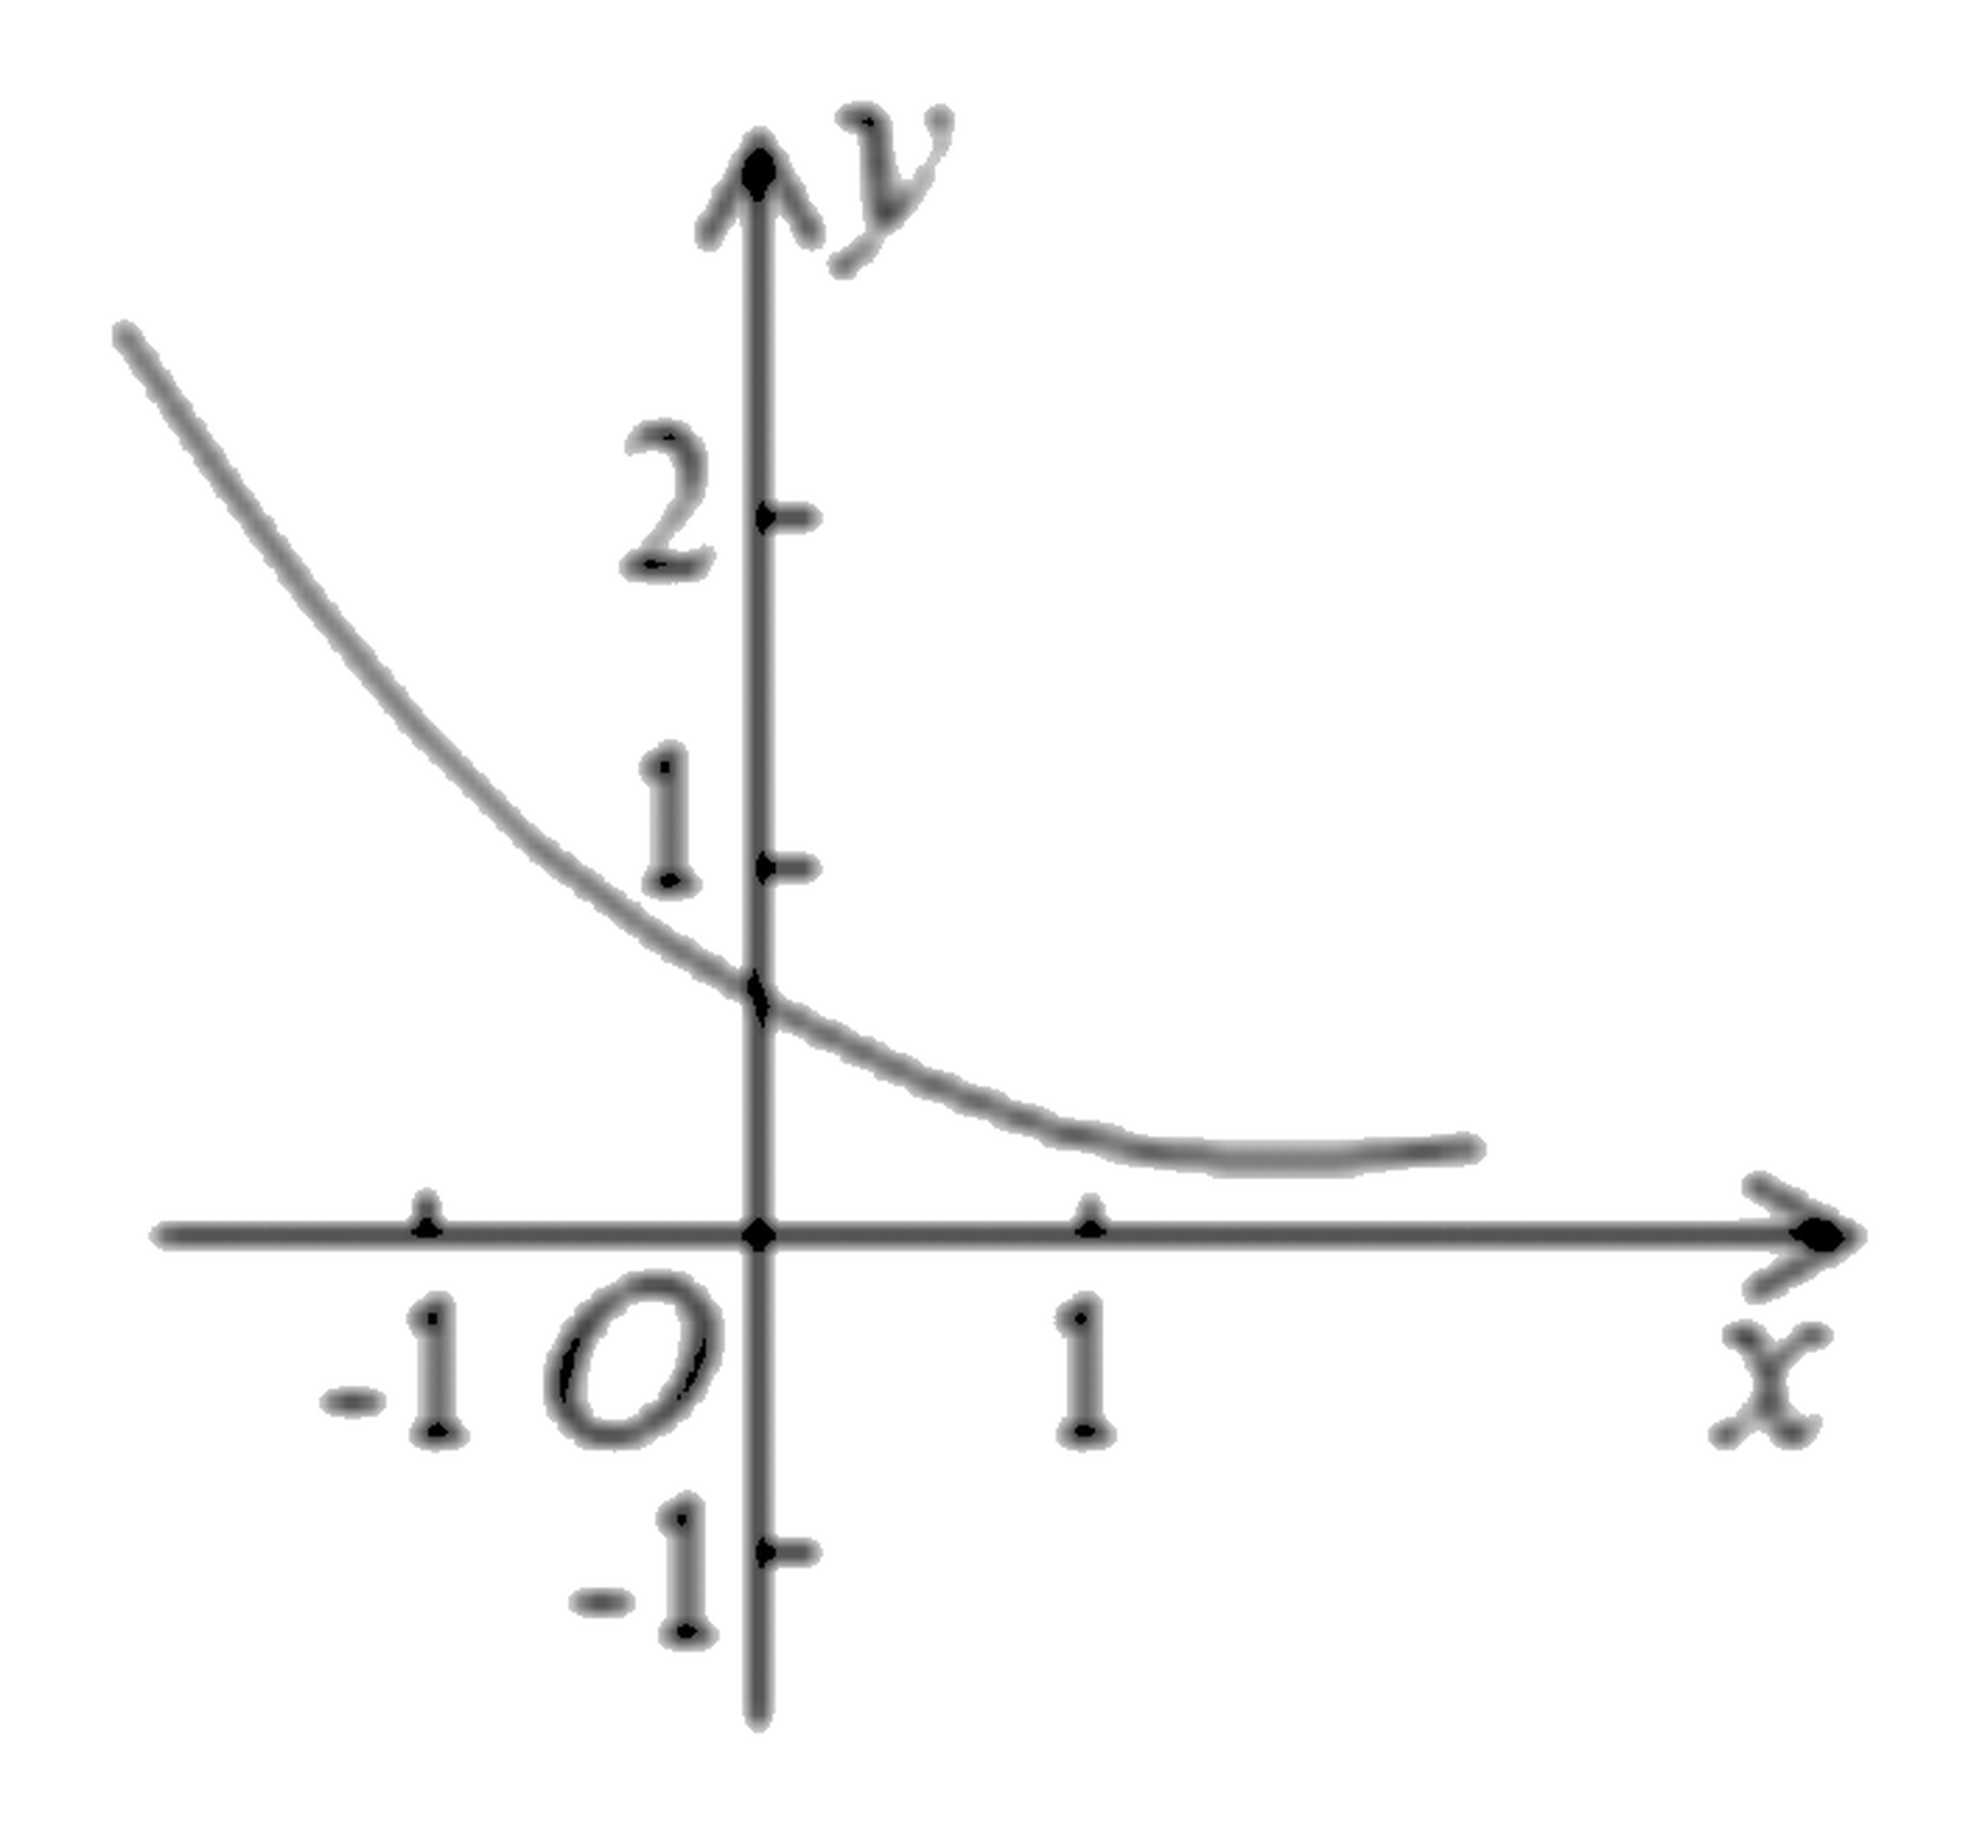
\includegraphics[width=0.30\textwidth]{figures/gao147_q15.png}
\end{center}

\ifanswer
\solbegin
\step{由图象从左到右下降得 $0<a<1$；}
\step{由图象与 $y$ 轴的交点得 $0<a^{-b}<1$，故 $b<0$；}
\step{故 $0<a<1$，$b<0$；故选 $D$.}
\solend
\fi

% === Q16 ===：位数新定义题（无弯引号，放大 04 页 z/q16_stem.png 确认）；四选项横排一行；解析 3 个印刷行
\item 数学运算是指在明晰运算对象的基础上，依据运算法则解决数学问题的素养. 因为运算，数的威力无限；没有运算，数就只是一个符号，对数运算与指数运算是两类重要的运算，对数的运算性质降低了运算的级别，简化了运算，在数学发展史上是伟大的成就. 而位数是指一个自然数有效位的个数，例如：$2^{10}=1024$，所以 $2^{10}$ 的位数为 4. 请你运用所学过的对数运算的知识，估计 $2025^{2026}$ 的位数是\mbox{（\quad）}

\keepwithprev
A. 6697\qquad B. 6698\qquad C. 6699\qquad D. 6700

\ifanswer
\solbegin
\step{设 $2025^{2026}=t$，所以 $\lg t=2026\lg2025$，}
\step{因为 $\lg2025\approx3.3064$，所以 $\lg t\approx6698.8$，}
\step{所以 $t\approx10^{6698.8}\in(10^{6698},10^{6699})$，所以 $2025^{2026}$ 的位数为 6699. 故选 $C$.}
\solend
\fi

\end{enumerate}

\bigsec{三、解答题}

\begin{enumerate}
\setcounter{enumi}{16}

% === Q17 ===：题干＋解析均在 04 页；集合描述竖线 \mid、描述内半角逗号照录；
% 空集 \varnothing、子集 \subseteq（放大 04 页 z/subset_04_q17b.png 确认带下划线）、数集 \R；
% 解析 5 个印刷行，首行末"所以 A=(-∞,-2)∪(3,+∞)"原卷无标点，照录不补
\item 已知集合 $A=\left\{x\mid \dfrac{x+2}{x-3}>0,x\in\R\right\}$，$B=\{x\mid \lvert x-2a\rvert\leqslant2,x\in\R\}$.

(1) 若 $a=1$，求 $A\cap B$；

(2) 若 $A\cap B=\varnothing$，求实数 $a$ 的取值范围.

\ifanswer
\solbegin
\step{由 $\dfrac{x+2}{x-3}>0$，得 $x<-2$ 或 $x>3$，所以 $A=(-\infty,-2)\cup(3,+\infty)$}
\step{(1) 当 $a=1$ 时，$B=\{x\mid \lvert x-2\rvert\leqslant2\}=[0,4]$，于是 $A\cap B=(3,4]$；}
\step{(2) $B=[2a-2,2a+2]$，}
\step{则 $A\cap B=\varnothing\Leftrightarrow[2a-2,2a+2]\subseteq[-2,3]\Leftrightarrow\begin{cases}2a-2\geqslant-2\\2a+2\leqslant3\end{cases}\Leftrightarrow0\leqslant a\leqslant\dfrac{1}{2}$，}
\step{所以实数 $a$ 的取值范围为 $\left[0,\dfrac{1}{2}\right]$.}
\solend
\fi

% === Q18 ===：氟化物／臭氧应用题；"氟化物""（如冰箱等）"全角夹注照录（放大 05 页 z/q18_line1.png 确认）；
% 关系式 $Q=Q_0e^{-0.0025t}$ 原卷独立一行，按一段照录；解析 6 个印刷行
\item 有些家用电器（如冰箱等）使用了氟化物，氟化物的释放破坏了大气上层的臭氧层，使臭氧含量 $Q$ 呈指数函数型变化，在氟化物排放量维持某种水平时，具有关系式

$Q=Q_0e^{-0.0025t}$，其中 $Q_0$ 是臭氧的初始量.

(1) 随时间 $t$ 的增加，臭氧的含量是增加还是减少？

(2) 试估计多少年以后将会有一半的臭氧消失.（用计算器计算）

\ifanswer
\solbegin
\step{(1) 对于函数 $Q=Q_0e^{-0.0025t}$，显然 $Q>0$，}
\step{任取 $t_1$、$t_2\in(0,+\infty)$，且 $t_1<t_2$，则 $t_2-t_1>0$，}
\step{所以 $\dfrac{Q_1}{Q_2}=\dfrac{Q_0e^{-0.0025t_1}}{Q_0e^{-0.0025t_2}}=e^{-0.0025(t_1-t_2)}=e^{0.0025(t_2-t_1)}>e^0=1$，所以 $Q_1>Q_2$，}
\step{故随着时间 $t$ 的增加，臭氧的含量是减少的；}
\step{(2) 令 $\dfrac{Q}{Q_0}=\dfrac{1}{2}$，即 $\dfrac{Q_0e^{-0.0025t}}{Q_0}=e^{-0.0025t}=\dfrac{1}{2}$，得 $-0.0025t=\ln\dfrac{1}{2}\approx-0.6931$，}
\step{解得 $t\approx277$，故估计 277 年以后将会有一半的臭氧消失.}
\solend
\fi

% === Q19 ===：题干用"图像"、解析两处用"图象"逐处照录不统一（05 页）；数集 \Z；
% 题干＋解析前 4 行在 05 页、解析后 3 行在 06 页；解析共 7 个印刷行
\item 已知幂函数 $f(x)=x^{-m^2+4m}(m\in\Z)$ 的图像关于 $y$ 轴对称，且在区间 $(0,+\infty)$ 上是严格增函数.

(1) 求 $m$ 的值；

(2) 求满足不等式 $(2a+1)^m<(a+1)^m$ 的实数 $a$ 的取值范围.

\ifanswer
\solbegin
\step{(1) 由题意得 $-m^2+4m>0$，解得 $0<m<4$，}
\step{因为 $m\in\Z$，所以 $m=1$ 或 $m=2$ 或 $m=3$.}
\step{当 $m=1$ 或 $m=3$ 时，$f(x)=x^3$，图象关于原点对称，不合题意；}
\step{当 $m=2$ 时，$f(x)=x^4$，图象关于 $y$ 轴对称，符合题意，所以 $m=2$.}
\step{(2) 代入 $m=2$，不等式为 $(2a+1)^2<(a+1)^2$，}
\step{得 $(2a+1)^2-(a+1)^2=a(3a+2)<0$，因此 $-\dfrac{2}{3}<a<0$，}
\step{所求范围为 $\left(-\dfrac{2}{3},0\right)$.}
\solend
\fi

% === Q20 ===：指数函数题，题干用"图像"；(3) 长求和式（分数 1/2026、1011/2026、2011/2026、
% 15/2026、1015/2026、2025/2026 放大 06 页 z/q20_sum_06a.png 确认）；题干在 06 页、
% 解析前 6 行在 06 页下半、后 6 行在 07 页上半；解析共 12 个印刷行
\item 已知指数函数 $y=a^x$（$a>0,a\ne1$）的图像经过点 $(1,4)$.

(1) 求实数 $a$ 的值；

(2) 若 $f(x)=(a^x)^2-2\cdot a^x-8$，当 $x\in\R$ 时，不等式 $f(x)>m\cdot4^x-12$ 恒成立，求 $m$ 的取值范围；

(3) 记 $g(x)=\dfrac{1}{a^x+2}$，求证：$g(x)+g(1-x)$ 为定值，并求 $g(0)+g\left(\dfrac{1}{2026}\right)+g\left(\dfrac{1011}{2026}\right)+g\left(\dfrac{2011}{2026}\right)+g\left(\dfrac{1}{2}\right)+g\left(\dfrac{15}{2026}\right)+g\left(\dfrac{1015}{2026}\right)+g\left(\dfrac{2025}{2026}\right)+g(1)$ 的值.

\ifanswer
\solbegin
\step{(1) 将 $(1,4)$ 代入 $y=a^x$，得 $a^1=4$，即 $a=4$.}
\step{(2) 令 $t=4^x$，当 $x\in\R$ 时，$t$ 取遍所有正实数.}
\step{原不等式等价于 $t^2-2t-8>mt-12\Leftrightarrow m<t+\dfrac{4}{t}-2$，}
\step{由基本不等式，$t+\dfrac{4}{t}-2\geqslant2\sqrt{t\cdot\dfrac{4}{t}}-2=2$，}
\step{当且仅当 $t=\dfrac{4}{t}$，即 $t=2$ 时取等号，}
\step{因此原不等式恒成立的充要条件为 $m<2$，即 $m\in(-\infty,2)$.}
\step{(3) 对任意 $x\in\R$，令 $t=4^x>0$，则 $4^{1-x}=\dfrac{4}{t}$，}
\step{从而 $g(x)+g(1-x)=\dfrac{1}{t+2}+\dfrac{1}{\dfrac{4}{t}+2}=\dfrac{1}{t+2}+\dfrac{t}{2(t+2)}=\dfrac{1}{2}$，}
\step{因此 $g(x)+g(1-x)$ 为定值 $\dfrac{1}{2}$.}
\step{原式中，0 与 1、$\dfrac{1}{2026}$ 与 $\dfrac{2025}{2026}$、$\dfrac{1011}{2026}$ 与 $\dfrac{1015}{2026}$、$\dfrac{2011}{2026}$ 与 $\dfrac{15}{2026}$}
\step{分别配对，每对函数值之和均为 $\dfrac{1}{2}$，且 $g\left(\dfrac{1}{2}\right)=\dfrac{1}{4^{\frac12}+2}=\dfrac{1}{4}$，}
\step{所以所求和为 $4\cdot\dfrac{1}{2}+\dfrac{1}{4}=\dfrac{9}{4}$.}
\solend
\fi

% === Q21 ===：不动点新定义题；题干在 07 页、解析续 08／09 页，共 20 个印刷行；
% 判别式两形混用：08 页 (2) cases 内等腰偏高 \Delta、09 页 (3) 扁等边 \triangle，逐处照录不统一
% （放大 /tmp/gao147/z/delta_vs_triangle.png 并排确认）；数集 \R；\forall 照录；
% 第 6—8 行是原卷一个长算式折成的三个印刷行，按印刷行分三条 \step、不并折行
\item 对于二次函数 $y=mx^2+nx+t(m\ne0)$，若存在 $x_0\in\R$，使得 $mx_0^2+nx_0+t=x_0$ 成立，则称 $x_0$ 为二次函数 $y=mx^2+nx+t(m\ne0)$ 的不动点.

(1) 求二次函数 $y=x^2-x-3$ 的不动点；

(2) 若二次函数 $y=2x^2-(3+a)x+a-1$ 有两个不相等的不动点 $x_1$、$x_2$，且 $x_1$、$x_2>0$，求 $\dfrac{x_1}{x_2}+\dfrac{x_2}{x_1}$ 的最小值；

(3) 若对任意实数 $b$，二次函数 $y=ax^2+(b+1)x+(b-1)(a\ne0)$ 恒有不动点，求 $a$ 的取值范围.

\ifanswer
\solbegin
\step{(1) 令 $x^2-x-3=x$，即 $x^2-2x-3=0$，即 $(x-3)(x+1)=0$，}
\step{解得 $x_1=-1$，$x_2=3$，所以不动点为 $-1$ 和 $3$.}
\step{(2) 由题意，$2x^2-(3+a)x+a-1=x$ 有两个不相等的正实数根，}
\step{即方程 $2x^2-(4+a)x+a-1=0$ 有两个不相等的正实数根，}
\step{所以 $\begin{cases}\Delta=(4+a)^2-8(a-1)>0\\x_1+x_2=\dfrac{4+a}{2}>0\\x_1\cdot x_2=\dfrac{a-1}{2}>0\end{cases}$，解得 $a>1$，}% 判别式原卷印等腰偏高粗三角 $\Delta$（放大 08 页 z/delta_08_q21cases.png）
\step{所以 $\dfrac{x_1}{x_2}+\dfrac{x_2}{x_1}=\dfrac{x_1^2+x_2^2}{x_1\cdot x_2}=\dfrac{(x_1+x_2)^2-2x_1\cdot x_2}{x_1\cdot x_2}=\dfrac{(x_1+x_2)^2}{x_1\cdot x_2}-2$}
\step{$=\dfrac{\left(\dfrac{4+a}{2}\right)^2}{\dfrac{a-1}{2}}-2=\dfrac{\dfrac{(a+4)^2}{4}}{\dfrac{a-1}{2}}-2=\dfrac{(a-1+5)^2}{2(a-1)}-2$}
\step{$=\dfrac{(a-1)^2+10(a-1)+25}{2(a-1)}-2=\dfrac{a-1}{2}+\dfrac{25}{2(a-1)}+3$.}
\step{因为 $a>1$，所以 $a-1>0$，}
\step{所以 $\dfrac{a-1}{2}+\dfrac{25}{2(a-1)}+3\geqslant2\sqrt{\dfrac{a-1}{2}\cdot\dfrac{25}{2(a-1)}}+3=8$，}
\step{当且仅当 $\dfrac{a-1}{2}=\dfrac{25}{2(a-1)}$，即 $a=6$ 时等号成立，}
\step{所以 $\dfrac{x_1}{x_2}+\dfrac{x_2}{x_1}$ 的最小值为 $8$.}
\step{(3) 设 $f(x)=ax^2+(b+1)x+b-1$，}
\step{则方程 $f(x)=x$，可化为 $ax^2+(b+1)x+b-1=x$，}
\step{即 $ax^2+bx+b-1=0$，}
\step{由题意得一元二次方程 $ax^2+bx+b-1=0$ 有解，又 $a\ne0$，}
\step{所以方程 $ax^2+bx+b-1=0$ 的判别式 $\triangle=b^2-4a(b-1)\geqslant0$，}% 判别式原卷印扁等边细线三角 $\triangle$（放大 09 页 z/triangle_09_q21.png），与 (2) 高 $\Delta$ 混用、照录不统一
\step{即 $b^2-4ab+4a\geqslant0$，则该不等式对 $\forall b\in\R$ 恒成立，}
\step{则 $(4a)^2-4\times4a\leqslant0$，且 $a\ne0$，解得 $0<a\leqslant1$，}
\step{所以实数 $a$ 的取值范围是 $(0,1]$.}
\solend
\fi

\end{enumerate}

\end{document}
"
% 紧凑版：xelatex "\def\iscompact{1}% 高一147_华师大三附中_期中.tex
%   —— 高一上数学"2026-2027 年华师大三附中高一上期中"（试卷版/答案版/紧凑版）
% 试卷版：xelatex 高一147_华师大三附中_期中.tex
% 答案版：xelatex "\def\isanswer{1}\input{高一147_华师大三附中_期中.tex}"
% 紧凑版：xelatex "\def\iscompact{1}\input{高一147_华师大三附中_期中.tex}"
%
% ① 原始材料：微信公众号"魔都数学加油站"文章，连载"27学年高一147"，原文标题
% "27学年高一147——2026-2027年上海市华师大三附中高一上期中"；
% 原文链接：https://mp.weixin.qq.com/s/X_gPW1JWoTAl2Bky_xEEGw 。
% 正文为 9 张 PNG 页（01/06/08/09 为 2560×3620，02/03/04/05/07 为 4762×6735，
% 同一篇各页分辨率混排，逐页按各自分辨率裁图核对，别按预览比例换算裁框）。
% 体例：混合体例讲评版——19 题中 Q4/Q5/Q7/Q9 只印【答案】、无【解析】，其余 15 题印
% 【解析】（逐题核实，见 ② ②）。题目、答案、解析均据原图转录；卷面粉红色水印
% "魔都数学加油站"及公众号页脚未录入。
% 全卷插图清单（逐页通读 9 页确认）：仅 1 处题目配图——
%   · Q15 递减指数函数小坐标系（03 页右侧：坐标轴、y 轴刻度 2/1/-1、x 轴刻度 -1/1、
%     原点 O、x/y 轴标），为"图像如图所示"的题目配图（选择题选项旁），三版都出；
%     裁自 03 页去粉色水印、去色、4× LANCZOS 放大存 figures/gao147_q15.png；
%   其余 8 页逐页确认无其它题目配图、无【解析】内配图、无表格，
%   亦无"题干写如图而源码漏图"一处；Q12/Q17/Q21 的 cases 块为数学块（非图）。
%
% 卷首标题：原卷印作"2026-2027 年华师大三附中高一上期中"，年份区间按全稿惯例排 en dash；
% 原卷卷面未印副标题，本稿按同期中卷（高一140／141／143／144／145／146）知识模块口径
% 补出"集合与常用逻辑用语、不等式、函数"。
%
% 题号体例（逐页核实定稿）：本卷共 19 题——一、填空题 3—12（10 题）、
% 二、选择题 13—16（4 题）、三、解答题 17—21（5 题）。
% 三节分别 \setcounter{enumi}{2}／{12}／{16}。原卷从第 3 题起、无第 1、2 题，
% 本稿保留原题号；全卷无附加题节（Q21 解析末行"所以实数 a 的取值范围是 (0,1]."
% 为全卷收尾，09 页下半仅水印、无正文）。
%
% ② 与原卷的排版差异：
%   ① 原文从第 3 题起，本稿保留原题号；共 19 题三节；
%   ② 混合体例：原卷 Q4/Q5/Q7/Q9 只印【答案】、无【解析】（分别为 a≤0、(-1,2)、
%      真、(-∞,1)），按 高一140 第 5 题／高一145 Q3 成例提 \ans{}、不补造解析；
%      其余 15 题印【解析】，用 \solbegin…\solend，选择题答案在解析末句"故选 X"
%      （Q13 选 B、Q14 选 B、Q15 选 D、Q16 选 C，逐个放大原图核实）、题干括号
%      \mbox{（\quad）} 留空、不另提 \ans{}；填空／解答答案落在解析里；
%      答案版【答案】/【解析】标记数 = 19（4 个 \ans ＋ 15 个 \solbegin）= 全卷题数；
%   ③ 原卷卷面未印副标题，本稿按知识模块口径补出；
%   ④ 原卷填空横线按全稿惯例排 \blankline[4.4em]；选择题括号排 \mbox{（\quad）}、
%      选项段前按惯例加 \keepwithprev；Q14／Q15 四选项为 2×2 两印刷行（A/B 一行、
%      C/D 一行），用空行分段照录（非一行 \qquad、亦非竖排四行）；解答题不留作答区、
%      不加 \anspace（原卷为讲评版，与 129／131／132／133／136／140／141／143／144／145／146 同）；
%   ⑤ 数集：Q4"A∪B=R"、Q13"f(x)=x^3 在 R 上严格增"、Q17"x∈R"两处、
%      Q20"x∈R"两处、Q21"x_0∈R""∀b∈R"原卷印斜体或黑板粗体 R，按全稿惯例统一改 \R；
%      Q19"m∈Z"改 \Z；本卷未出现 N（\N^* 无对应处）。绝对值排 \lvert…\rvert，
%      集合描述竖线排 \mid；不等号按全稿惯例排 \leqslant／\geqslant（原卷印 \le／\ge 形，
%      【答案】a≤0 亦排 \leqslant）；空集 \varnothing（Q17 两处）；
%      子集 \subseteq（Q17 带下划线，放大 04 页确认）；本卷未出现 \subset／\subsetneq，
%      亦未出现补集上划线 \overline{}；\left…\right 不得拆到不同 $…$ 组；
%   ⑥ 子题标号 (1)(2)(3) 半角括号照录；cases 块整体算一个印刷行（Q3、Q12 一行内
%      两个 cases、Q17、Q21(2)）；本卷解析内无圈数字①②③（无 \text{①} 需求）；
%      数学式内 CJK 用 \text{}（本卷未见）；
%   ⑦ 题干中的中文弯引号按原卷照录：Q7 命题"若 A∪B=B，则 A∩B=A"与
%      (填 " 真 " 或 " 假 ")、Q10 (填 ">" "<" "≤" "或≥")，含引号内空格；
%      注释内一律 ASCII 引号；Q16 位数新定义题逐字放大确认无弯引号
%      （交办提示的"Q16 新定义题"举例未在本卷出现），未补造引号；
%   ⑧ 半角逗号在数学组之间是全稿惯例、非笔误（Q4"$A=(-\infty,0],B=[a,+\infty)$"、
%      Q5"$(a>0,a\ne1)$"、Q17 集合描述内"$>0,x\in R$""$\leqslant2,x\in R$"、
%      Q20 题干"$(a>0,a\ne1)$"、Q21"$y=mx^2+nx+t(m\ne0)$"等），逐处照录别改全角；
%      行末西文句点照录为 ASCII `.`；行中全角逗号／顿号照录；
%      Q7／Q10"(填…)"为半角括号、Q18"（如冰箱等）"为全角括号，逐处照录不统一；
%   ⑨ "图像／图象"逐处照录不统一：题干 5 处用"图像"（Q5"图像恒过定点"、
%      Q9"图像位于直线 y=x 的下方"、Q15"的图像如图所示"、Q19"的图像关于 y 轴对称"、
%      Q20"的图像经过点"），解析 4 处用"图象"（Q15"由图象从左到右下降"
%      "由图象与 y 轴的交点"、Q19"图象关于原点对称""图象关于 y 轴对称"），逐处核、不统一；
%   ⑩ 判别式 Δ/△ 混用是照录项：Q21(2) 解析 cases 块"Δ=(4+a)²−8(a−1)>0"
%      印等腰偏高粗三角 \Delta，Q21(3) 解析"判别式△=b²−4a(b−1)≥0"
%      印扁等边细线三角 \triangle，逐处放大判断、照录不得统一
%      （参照 高一142／144／145 头注④口径，详见 ④）；
%   ⑪ 一条 \step = 原卷解析的一个印刷行，cases 块整体算一个印刷行；别把原卷折行
%      并起来、别把一行拆多条。Q10 七行（跨 01→02 页）、Q12 七行（含一行两 cases）、
%      Q20 十二行（含"原式中…2011/2026 与 15/2026／分别配对…"折行两行）、
%      Q21 二十行（含第 6—8 行一个长算式折成三印刷行、含 cases）均按印刷行逐条断，
%      不丢行；
%   ⑫ 配图：逐页通读 9 页确认全卷仅 Q15 一处题目配图（见 ①），三版都出、
%      \includegraphics[width=0.30\textwidth]；图块较小，未加 \needvspace 大图块守卫
%      （仅 \bigsec 自带 \needvspace{3\baselineskip}）；三版切页审计均"合计异常：无"；
%   ⑬ 跨页续印按题合并：Q3—Q9 在 01 页（Q10 题干在 01 页末、解析首行亦在 01 页末）；
%      Q10 解析续 02 页 6 行、Q11 在 02 页、Q12 题干＋解析前 4 行在 02 页
%      （解析续 03 页 3 行）；"二、选择题"标题与 Q13、Q14、Q15 题干＋解析前 2 行在 03 页
%      （Q15 配图在 03 页右侧）；Q15 解析末行与 Q16、"三、解答题"标题、Q17 在 04 页；
%      Q18 在 05 页、Q19 题干＋解析前 4 行在 05 页（解析续 06 页 3 行）；
%      Q20 题干＋解析前 6 行在 06 页（解析续 07 页 6 行）、Q21 题干＋解析前 3 行在 07 页；
%      Q21 解析续 08 页 13 行、续 09 页 4 行（09 页下半仅水印、无正文）。
%      本稿按题连排，不丢行、不并折行；
%   ⑭ 原卷解析内无红色"法一／法二"之类小标题，故本卷无 \stepm；
%      水印"魔都数学加油站"红色不录入。
%
% ③ 行数复核：一条 \step／\stepm = 原卷解析的一个印刷行，cases 块作一个印刷行计。
%   逐题数（主会话逐页核对定稿）：Q3：1；Q4：0（只印【答案】、提 \ans{}，不计入 \step 账）；
%   Q5：0；Q6：1；Q7：0；Q8：2；Q9：0；Q10：7；Q11：4；Q12：7；Q13：6；Q14：4；
%   Q15：3；Q16：3；Q17：5；Q18：6；Q19：7；Q20：12；Q21：20。
%   合计 88 条 \step（本卷无 \stepm：解析内无红色"法一／法二"类小标题），
%   与原卷逐题印刷行相等。全卷 15 题设 \solbegin…\solend ＋ 4 题一处 \ans{}，
%   答案版【答案】/【解析】标记数 = 19 = 全卷题数。
%
% ④ 判别式／子集符号结论（逐处放大原图照录、不得统一，主会话像素级复核）：
%   判别式全卷 2 处、两形混用逐处照录不统一（参照 高一142／144 头注④口径）：
%     · Q21(2) 解析 cases 块"Δ=(4+a)²−8(a−1)>0" 原卷印等腰偏高粗三角
%       （高>宽、粗笔画），照录 \Delta（放大 08 页 /tmp/gao147/z/delta_08_q21cases.png
%       与 z/delta_vs_triangle.png 左图确认）；
%     · Q21(3) 解析"判别式△=b²−4a(b−1)≥0" 原卷印扁等边细线三角
%       （宽≈高、细线），照录 \triangle（放大 09 页 /tmp/gao147/z/triangle_09_q21.png
%       与 z/delta_vs_triangle.png 右图并排确认）。
%   子集／补集：Q17 解析"[2a−2,2a+2]⊆[−2,3]" 原卷印带下划线 ⊆，照录 \subseteq
%     （放大 04 页 /tmp/gao147/z/subset_04_q17b.png 确认）；Q17"A∩B=∅"空集 \varnothing；
%     集合描述竖线 \mid（Q10 M、Q12 解集、Q17 A/B）；并集 \cup（Q4、Q17）、
%     交集 \cap（Q7、Q17）、不属于 \notin（Q10）；数集 \R／\Z 归一见 ② ⑤。
%   本卷未出现 \subset／\subsetneq，未出现补集上划线 \overline{}。
%
% ⑤ 存疑照录（放大原图确认，照录未改、正文对应处另有 % 注）：
%   1. Q4/Q5/Q7/Q9 只印【答案】、无【解析】，按成例提 \ans{}、不补造解析
%      （混合体例逐题核实，见 ② ②）。
%   2. Q21(2) 判别式高 \Delta 与 Q21(3) 判别式扁 \triangle 两形混用，
%      逐处照录不统一（见 ④）。
%   3. "图像／图象"题干 5 处"图像"、解析 4 处"图象"，逐处照录不统一（见 ② ⑨）。
%   4. Q7／Q10"(填…)"半角括号与 Q18"（如冰箱等）"全角括号，逐处照录不统一。
%   5. Q16 位数新定义题逐字放大确认无弯引号（交办提示的"Q16 新定义题"举例
%      未在本卷出现），未补造引号；全卷弯引号仅 Q7、Q10 两处。
%   6. Q17 解析首行末"所以 A=(-∞,-2)∪(3,+∞)"、Q20(3) 解析"…2011/2026 与 15/2026"
%      行末原卷均无标点，照录未补；Q21(2) 第 6—8 行一个长算式折成三印刷行，
%      按印刷行分三条 \step、不并折行。
%   全卷除此 6 类外未发现其它笔误／自相矛盾处。
%
% ⑥ 跨页续印按题合并说明：见 ② ⑬。
%
\documentclass[a4paper,11pt]{article}
\usepackage{common}

\begin{document}

\examtitlest[3]{2026--2027 年华师大三附中高一上期中}{集合与常用逻辑用语、不等式、函数}

\bigsec{一、填空题}

\begin{enumerate}
\setcounter{enumi}{2}

% === Q3 ===：印【解析】，1 个印刷行（cases 块整体算一行）
\item 函数 $y=(a^2-5a+7)a^x+6-2a$ 是指数函数，则 $a$ 的值为\blankline[4.4em].

\ifanswer
\solbegin
\step{由题意得 $\begin{cases}a^2-5a+7=1\\6-2a=0\end{cases}$，解得 $a=3$.}
\solend
\fi

% === Q4 ===：原卷只印【答案】、无【解析】，按 高一140 第 5 题／高一145 Q3 成例提 \ans{}、不补造解析；
% 题干数学组内半角逗号 $A=(-\infty,0],B=[a,+\infty)$ 照录（放大 01 页 z/q4_stem.png 确认）
\item 已知 $A=(-\infty,0],B=[a,+\infty)$，且 $A\cup B=\R$，则实数 $a$ 的取值范围为\blankline[4.4em].

\ifanswer
\ans{$a\leqslant0$}
\fi

% === Q5 ===：只印【答案】；题干"图像"照录（放大 01 页 z/q5_stem.png 确认）；
% 数学组内半角逗号 $(a>0,a\ne1)$ 照录
\item 函数 $y=a^{x+1}+1(a>0,a\ne1)$ 的图像恒过定点\blankline[4.4em].

\ifanswer
\ans{$(-1,2)$}
\fi

% === Q6 ===：印【解析】，1 个印刷行
\item 已知方程 $x^2+2x-4=0$ 的两个根为 $x_1$、$x_2$，则 $x_1^2+x_2^2$ 的值为\blankline[4.4em].

\ifanswer
\solbegin
\step{$x_1^2+x_2^2=(x_1+x_2)^2-2x_1x_2=4+8=12$.}
\solend
\fi

% === Q7 ===：只印【答案】；中文弯引号"若 A∪B=B，则 A∩B=A"与(填 " 真 " 或 " 假 ")内的空格照录
% （放大 01 页 z/q7_quotes_7x.png、z/q7_tail.png 确认，括号为半角）
\item 命题 “若 $A\cup B=B$，则 $A\cap B=A$” 为\blankline[4.4em]命题(填 “ 真 ” 或 “ 假 ”).

\ifanswer
\ans{真}
\fi

% === Q8 ===：印【解析】，2 个印刷行；不等号按全稿惯例 \geqslant／\leqslant
\item 已知正实数 $a$、$b$ 满足 $a+4b=1$，则 $ab$ 的最大值为\blankline[4.4em].

\ifanswer
\solbegin
\step{$a+4b\geqslant2\sqrt{a\cdot4b}\Rightarrow ab\leqslant\dfrac{1}{16}$，当且仅当 $a=4b=\dfrac{1}{2}$ 时取等号，}
\step{则 $ab$ 的最大值为 $\dfrac{1}{16}$.}
\solend
\fi

% === Q9 ===：只印【答案】；题干"图像"照录（放大 01 页 hi_01_2 确认）
\item 若幂函数 $y=x^s$ 在 $x>1$ 时的图像位于直线 $y=x$ 的下方，则 $s$ 的取值范围是\blankline[4.4em].

\ifanswer
\ans{$(-\infty,1)$}
\fi

% === Q10 ===：印【解析】，共 7 个印刷行（题在 01 页末起 1 行、续 02 页 6 行）；
% 题干跨两印刷行"则 |ab|+1 ____ |a|+|b|（填…）"按一句连排；(填…)为半角括号、引号内空格照录
\item 已知不等式 $\lvert2x+1\rvert+\lvert2x-1\rvert<4$ 的解集为 $M$. 设实数 $a\in M$，$b\notin M$，则 $\lvert ab\rvert+1$\blankline[4.4em] $\lvert a\rvert+\lvert b\rvert$(填 “$>$”，“$<$”，“$\leqslant$” “或$\geqslant$”).

\ifanswer
\solbegin
\step{当 $x<-\dfrac{1}{2}$ 时，不等式化为 $-2x-1+1-2x<4$，即 $x>-1$，所以 $-1<x<-\dfrac{1}{2}$；}
\step{当 $-\dfrac{1}{2}\leqslant x\leqslant\dfrac{1}{2}$ 时，不等式化为 $2x+1-2x+1<4$，即 $2<4$，所以 $-\dfrac{1}{2}\leqslant x\leqslant\dfrac{1}{2}$；}
\step{当 $x>\dfrac{1}{2}$ 时，不等式化为 $2x+1+2x-1<4$，即 $x<1$，所以 $\dfrac{1}{2}<x<1$；}
\step{综上，$M=\{x\mid -1<x<1\}$.}
\step{因为 $a\in M$，$b\notin M$，所以 $\lvert a\rvert<1$，$\lvert b\rvert\geqslant1$.}
\step{而 $\lvert ab\rvert+1-(\lvert a\rvert+\lvert b\rvert)=\lvert ab\rvert+1-\lvert a\rvert-\lvert b\rvert=(\lvert a\rvert-1)(\lvert b\rvert-1)$，}
\step{所以 $\lvert ab\rvert+1\leqslant\lvert a\rvert+\lvert b\rvert$.}
\solend
\fi

% === Q11 ===：印【解析】，4 个印刷行（02 页）
\item 已知 $m>1$，$n>1$，$\lg m=\log_n100$，则 $mn$ 的最小值为\blankline[4.4em].

\ifanswer
\solbegin
\step{由 $m>1$，$n>1$，得 $\lg m>0$，$\lg n>0$，}
\step{因为 $\lg m=\log_n100=\dfrac{\lg100}{\lg n}=\dfrac{2}{\lg n}$，所以 $\lg m\cdot\lg n=2$，}
\step{所以 $\lg(mn)=\lg m+\lg n\geqslant2\sqrt{\lg m\cdot\lg n}=2\sqrt2$，}
\step{当且仅当 $m=n=10^{\sqrt2}$ 时取等号，则 $mn\geqslant10^{2\sqrt2}$，即 $mn$ 的最小值为 $10^{2\sqrt2}$.}
\solend
\fi

% === Q12 ===：印【解析】，共 7 个印刷行（02 页 4 行、03 页 3 行）；
% 第 3 行"则 [cases]，得 [cases]，"两个 cases 块同属一个印刷行，整体作一条 \step（照 高一146 Q11 成例）
\item 已知关于 $x$ 的不等式 $ax^2+bx+c\leqslant1$ 的解集为 $\{x\mid -1\leqslant x\leqslant3\}$. 若关于 $x$ 的不等式 $ax^2+(b-1)x+c-2\leqslant0$ 有且仅有 8 个整数解，则实数 $a$ 的取值范围是\blankline[4.4em].

\ifanswer
\solbegin
\step{由已知关于 $x$ 的不等式 $ax^2+bx+c\leqslant1$ 的解集为 $\{x\mid -1\leqslant x\leqslant3\}$，}
\step{得 $a>0$，且方程 $ax^2+bx+c-1=0$ 的两根分别为 $-1$ 和 $3$，}
\step{则 $\begin{cases}-1+3=-\dfrac{b}{a}\\-1\times3=\dfrac{c-1}{a}\end{cases}$，得 $\begin{cases}b=-2a\\c=1-3a\end{cases}$，}
\step{不等式 $ax^2+(b-1)x+c-2\leqslant0$ 等价于 $ax^2-(2a+1)x-(3a+1)\leqslant0$，}
\step{即 $\left[x-\left(3+\dfrac{1}{a}\right)\right](x+1)\leqslant0$，解得 $-1\leqslant x\leqslant3+\dfrac{1}{a}$，}
\step{因为关于 $x$ 的不等式 $ax^2+(b-1)x+c-2\leqslant0$ 有且仅有 8 个整数解，}
\step{因此 $6\leqslant3+\dfrac{1}{a}<7$，即 $3\leqslant\dfrac{1}{a}<4$，解得 $\dfrac{1}{4}<a\leqslant\dfrac{1}{3}$，所以 $a$ 的取值范围为 $\left(\dfrac{1}{4},\dfrac{1}{3}\right]$.}
\solend
\fi

\end{enumerate}

\bigsec{二、选择题}

\begin{enumerate}
\setcounter{enumi}{12}

% === Q13 ===：题干＋选项＋解析均在 03 页；四选项横排一行；解析 6 个印刷行，末句"故选 B."
\item $a<b<0$，则下列不等式能成立的是\mbox{（\quad）}

\keepwithprev
A. $\dfrac{a}{b}<1$\qquad B. $\lvert a\rvert>-b$\qquad C. $\dfrac{1}{a}<\dfrac{1}{b}$\qquad D. $b^3<a^3$

\ifanswer
\solbegin
\step{对于 $A$，令 $a=-4$，$b=-3$，满足 $a<b<0$，但 $\dfrac{a}{b}>1$，故 $A$ 错误，}
\step{对于 $B$，因为 $a<b<0$，所以 $-a>-b>0$，即 $\lvert a\rvert>-b$，故 $B$ 正确，}
\step{对于 $C$，令 $a=-4$，$b=-3$，满足 $a<b<0$，但 $\dfrac{1}{a}>\dfrac{1}{b}$，故 $C$ 错误，}
\step{对于 $D$，$f(x)=x^3$ 在 $\R$ 上严格增，因为 $a<b$，所以 $f(a)<f(b)$，}
\step{即 $a^3<b^3$，故 $D$ 错误.}
\step{故选 $B$.}
\solend
\fi

% === Q14 ===：四选项原卷为 2×2 两印刷行（A/B 一行、C/D 一行），用空行分段照录；解析 4 个印刷行
\item 已知 $a$、$b$ 为实数，若 $\alpha:ab=0$，$\beta:a^2+\sqrt{b}=0$，则 $\alpha$ 是 $\beta$ 的\mbox{（\quad）}

\keepwithprev
A. 充分不必要条件\qquad\qquad B. 必要不充分条件

C. 充要条件\qquad\qquad D. 既不充分也不必要条件

\ifanswer
\solbegin
\step{$\beta:a^2+\sqrt{b}=0$，所以 $a=0$ 且 $b=0$，}
\step{由 $a=0$，$b=0\Rightarrow ab=0$，反之不成立.}
\step{所以 $ab=0$ 是 $a=0$，$b=0$ 的必要不充分条件，即 $\alpha$ 是 $\beta$ 的必要不充分条件，}
\step{故选 $B$.}
\solend
\fi

% === Q15 ===：题目配图（03 页右侧小坐标系），三版都出；题干用"图像"、解析用"图象"逐处照录；
% 四选项 2×2 两印刷行；解析 3 个印刷行（03 页 2 行、04 页 1 行，末句"故选 D."与前行同一印刷行）
\item 函数 $f(x)=a^{x-b}$ 的图像如图所示，其中 $a$、$b$ 为常数，则下列结论正确的是\mbox{（\quad）}

\keepwithprev
A. $a>1$，$b<0$\qquad\qquad B. $a>1$，$b>0$

C. $0<a<1$，$b>0$\qquad\qquad D. $0<a<1$，$b<0$

\begin{center}
% 递减指数函数小坐标系图取 03 页右侧，去粉色水印、去色、4× LANCZOS 放大；题目配图三版都出
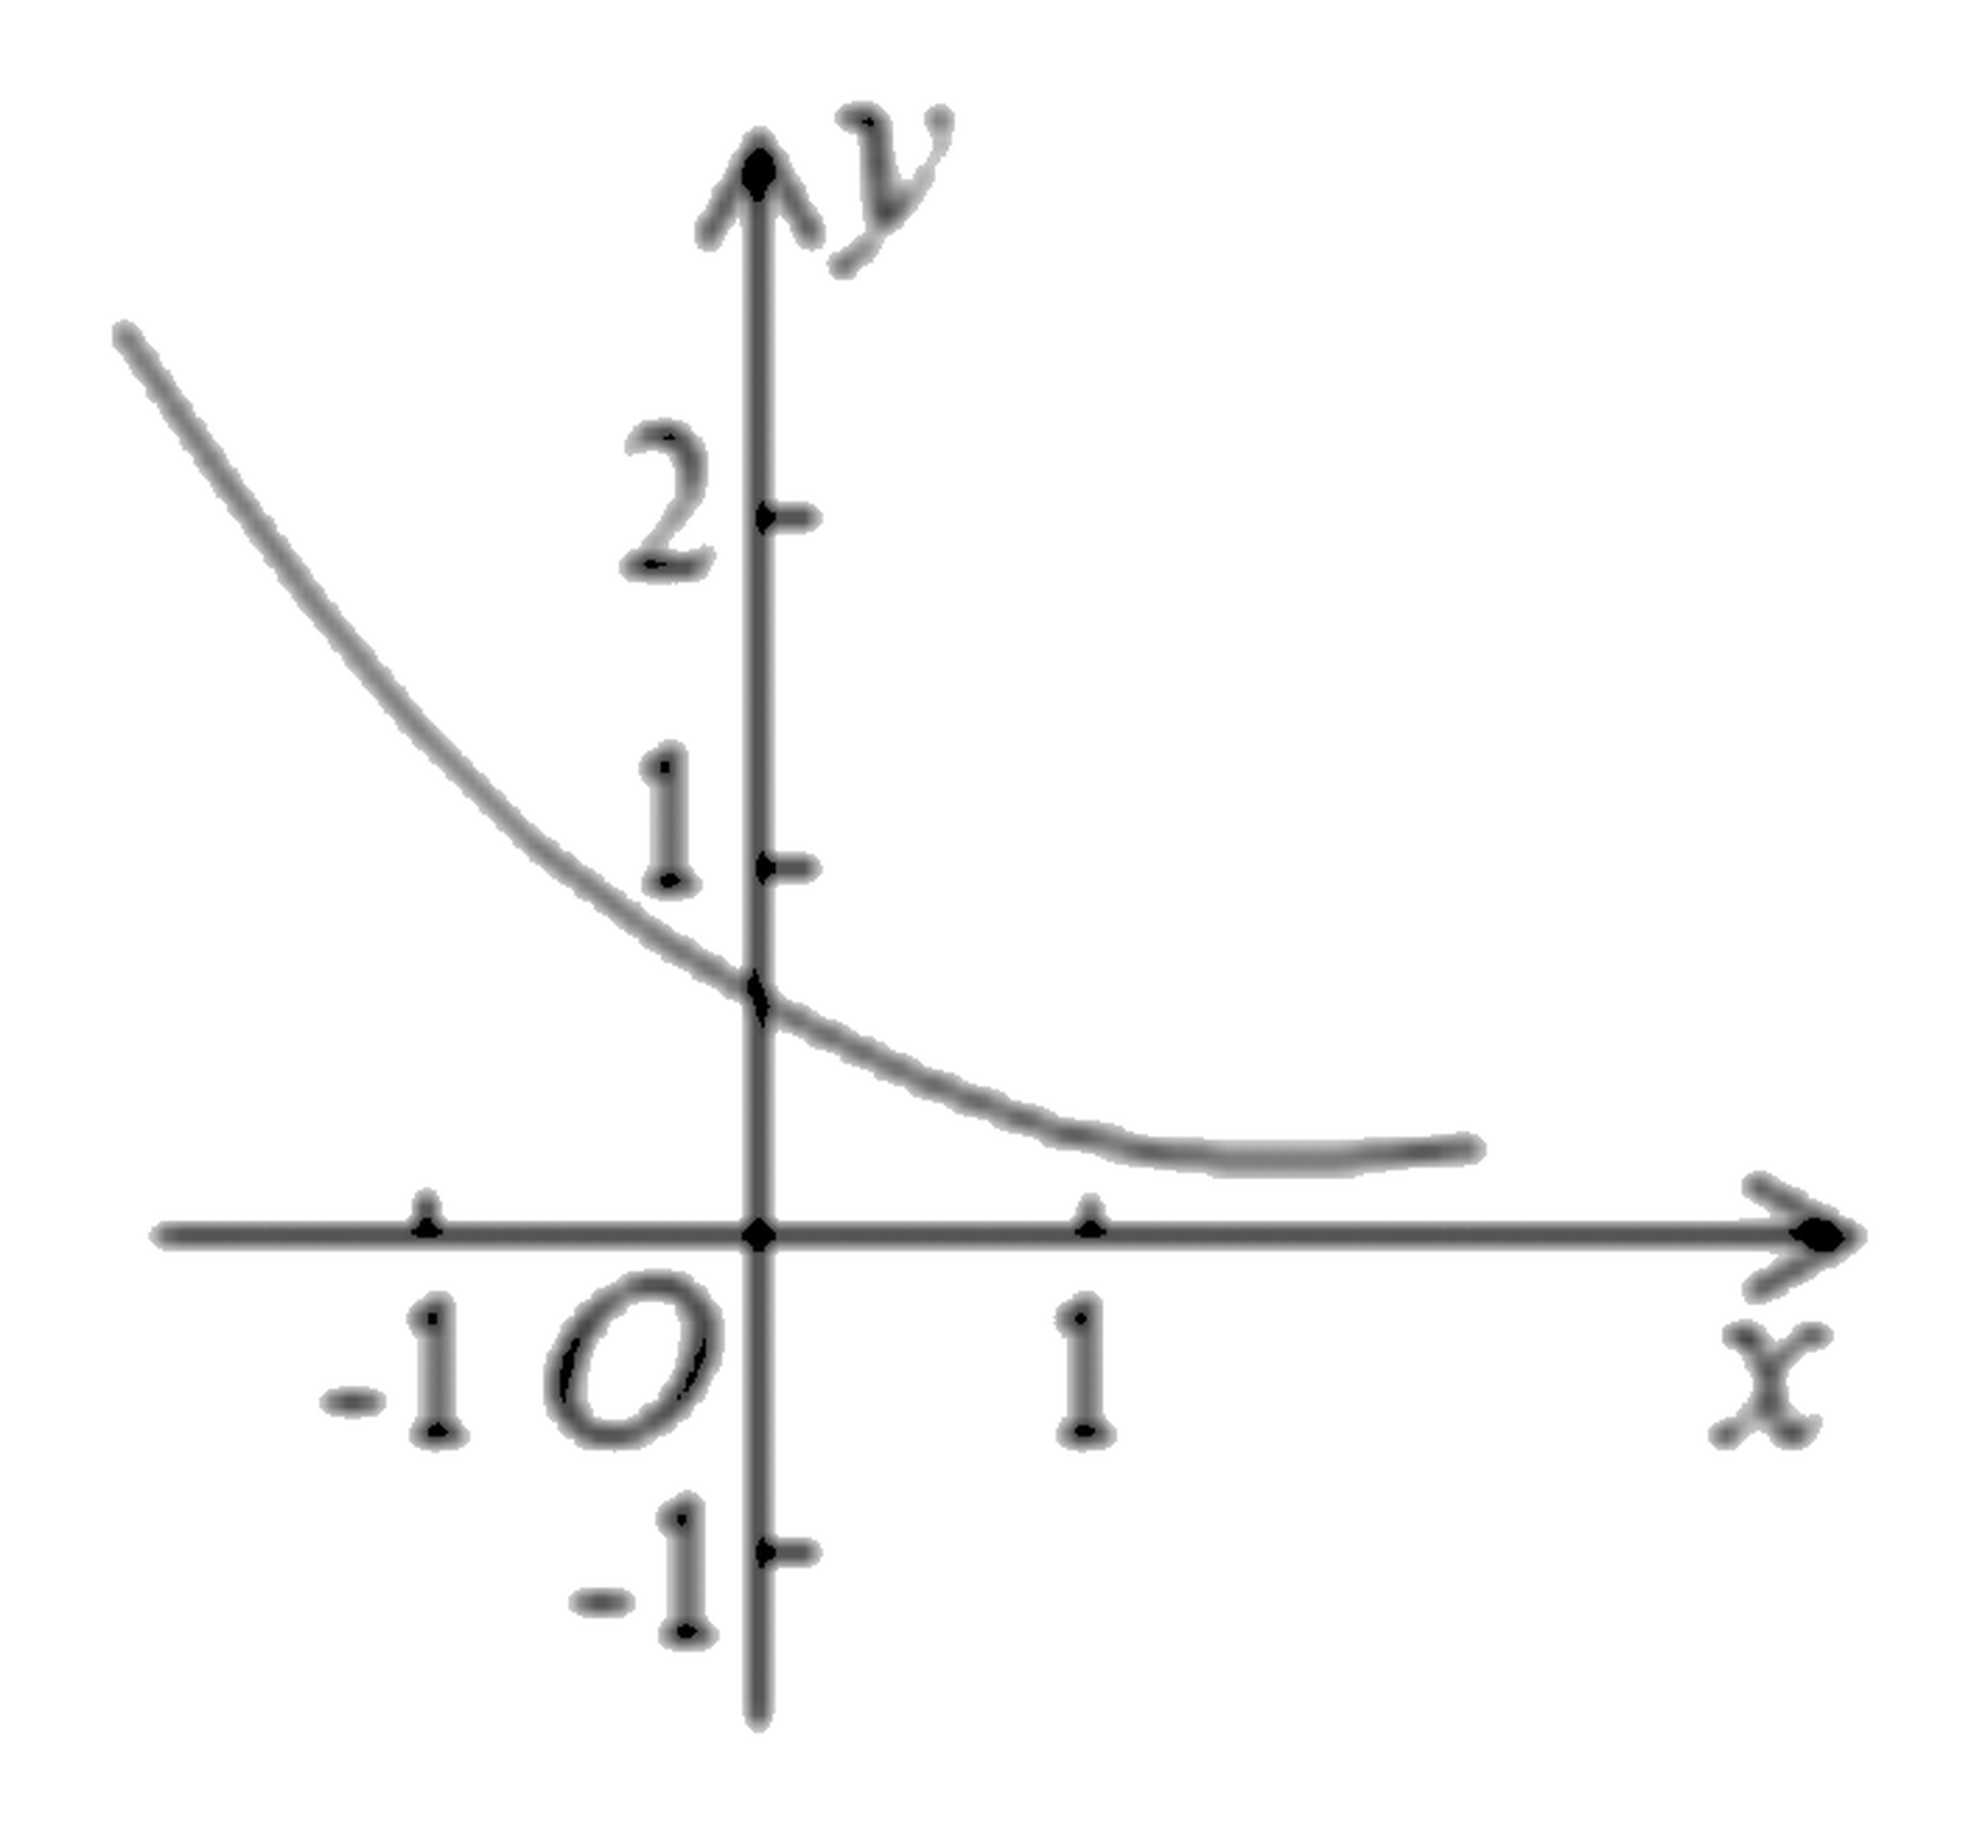
\includegraphics[width=0.30\textwidth]{figures/gao147_q15.png}
\end{center}

\ifanswer
\solbegin
\step{由图象从左到右下降得 $0<a<1$；}
\step{由图象与 $y$ 轴的交点得 $0<a^{-b}<1$，故 $b<0$；}
\step{故 $0<a<1$，$b<0$；故选 $D$.}
\solend
\fi

% === Q16 ===：位数新定义题（无弯引号，放大 04 页 z/q16_stem.png 确认）；四选项横排一行；解析 3 个印刷行
\item 数学运算是指在明晰运算对象的基础上，依据运算法则解决数学问题的素养. 因为运算，数的威力无限；没有运算，数就只是一个符号，对数运算与指数运算是两类重要的运算，对数的运算性质降低了运算的级别，简化了运算，在数学发展史上是伟大的成就. 而位数是指一个自然数有效位的个数，例如：$2^{10}=1024$，所以 $2^{10}$ 的位数为 4. 请你运用所学过的对数运算的知识，估计 $2025^{2026}$ 的位数是\mbox{（\quad）}

\keepwithprev
A. 6697\qquad B. 6698\qquad C. 6699\qquad D. 6700

\ifanswer
\solbegin
\step{设 $2025^{2026}=t$，所以 $\lg t=2026\lg2025$，}
\step{因为 $\lg2025\approx3.3064$，所以 $\lg t\approx6698.8$，}
\step{所以 $t\approx10^{6698.8}\in(10^{6698},10^{6699})$，所以 $2025^{2026}$ 的位数为 6699. 故选 $C$.}
\solend
\fi

\end{enumerate}

\bigsec{三、解答题}

\begin{enumerate}
\setcounter{enumi}{16}

% === Q17 ===：题干＋解析均在 04 页；集合描述竖线 \mid、描述内半角逗号照录；
% 空集 \varnothing、子集 \subseteq（放大 04 页 z/subset_04_q17b.png 确认带下划线）、数集 \R；
% 解析 5 个印刷行，首行末"所以 A=(-∞,-2)∪(3,+∞)"原卷无标点，照录不补
\item 已知集合 $A=\left\{x\mid \dfrac{x+2}{x-3}>0,x\in\R\right\}$，$B=\{x\mid \lvert x-2a\rvert\leqslant2,x\in\R\}$.

(1) 若 $a=1$，求 $A\cap B$；

(2) 若 $A\cap B=\varnothing$，求实数 $a$ 的取值范围.

\ifanswer
\solbegin
\step{由 $\dfrac{x+2}{x-3}>0$，得 $x<-2$ 或 $x>3$，所以 $A=(-\infty,-2)\cup(3,+\infty)$}
\step{(1) 当 $a=1$ 时，$B=\{x\mid \lvert x-2\rvert\leqslant2\}=[0,4]$，于是 $A\cap B=(3,4]$；}
\step{(2) $B=[2a-2,2a+2]$，}
\step{则 $A\cap B=\varnothing\Leftrightarrow[2a-2,2a+2]\subseteq[-2,3]\Leftrightarrow\begin{cases}2a-2\geqslant-2\\2a+2\leqslant3\end{cases}\Leftrightarrow0\leqslant a\leqslant\dfrac{1}{2}$，}
\step{所以实数 $a$ 的取值范围为 $\left[0,\dfrac{1}{2}\right]$.}
\solend
\fi

% === Q18 ===：氟化物／臭氧应用题；"氟化物""（如冰箱等）"全角夹注照录（放大 05 页 z/q18_line1.png 确认）；
% 关系式 $Q=Q_0e^{-0.0025t}$ 原卷独立一行，按一段照录；解析 6 个印刷行
\item 有些家用电器（如冰箱等）使用了氟化物，氟化物的释放破坏了大气上层的臭氧层，使臭氧含量 $Q$ 呈指数函数型变化，在氟化物排放量维持某种水平时，具有关系式

$Q=Q_0e^{-0.0025t}$，其中 $Q_0$ 是臭氧的初始量.

(1) 随时间 $t$ 的增加，臭氧的含量是增加还是减少？

(2) 试估计多少年以后将会有一半的臭氧消失.（用计算器计算）

\ifanswer
\solbegin
\step{(1) 对于函数 $Q=Q_0e^{-0.0025t}$，显然 $Q>0$，}
\step{任取 $t_1$、$t_2\in(0,+\infty)$，且 $t_1<t_2$，则 $t_2-t_1>0$，}
\step{所以 $\dfrac{Q_1}{Q_2}=\dfrac{Q_0e^{-0.0025t_1}}{Q_0e^{-0.0025t_2}}=e^{-0.0025(t_1-t_2)}=e^{0.0025(t_2-t_1)}>e^0=1$，所以 $Q_1>Q_2$，}
\step{故随着时间 $t$ 的增加，臭氧的含量是减少的；}
\step{(2) 令 $\dfrac{Q}{Q_0}=\dfrac{1}{2}$，即 $\dfrac{Q_0e^{-0.0025t}}{Q_0}=e^{-0.0025t}=\dfrac{1}{2}$，得 $-0.0025t=\ln\dfrac{1}{2}\approx-0.6931$，}
\step{解得 $t\approx277$，故估计 277 年以后将会有一半的臭氧消失.}
\solend
\fi

% === Q19 ===：题干用"图像"、解析两处用"图象"逐处照录不统一（05 页）；数集 \Z；
% 题干＋解析前 4 行在 05 页、解析后 3 行在 06 页；解析共 7 个印刷行
\item 已知幂函数 $f(x)=x^{-m^2+4m}(m\in\Z)$ 的图像关于 $y$ 轴对称，且在区间 $(0,+\infty)$ 上是严格增函数.

(1) 求 $m$ 的值；

(2) 求满足不等式 $(2a+1)^m<(a+1)^m$ 的实数 $a$ 的取值范围.

\ifanswer
\solbegin
\step{(1) 由题意得 $-m^2+4m>0$，解得 $0<m<4$，}
\step{因为 $m\in\Z$，所以 $m=1$ 或 $m=2$ 或 $m=3$.}
\step{当 $m=1$ 或 $m=3$ 时，$f(x)=x^3$，图象关于原点对称，不合题意；}
\step{当 $m=2$ 时，$f(x)=x^4$，图象关于 $y$ 轴对称，符合题意，所以 $m=2$.}
\step{(2) 代入 $m=2$，不等式为 $(2a+1)^2<(a+1)^2$，}
\step{得 $(2a+1)^2-(a+1)^2=a(3a+2)<0$，因此 $-\dfrac{2}{3}<a<0$，}
\step{所求范围为 $\left(-\dfrac{2}{3},0\right)$.}
\solend
\fi

% === Q20 ===：指数函数题，题干用"图像"；(3) 长求和式（分数 1/2026、1011/2026、2011/2026、
% 15/2026、1015/2026、2025/2026 放大 06 页 z/q20_sum_06a.png 确认）；题干在 06 页、
% 解析前 6 行在 06 页下半、后 6 行在 07 页上半；解析共 12 个印刷行
\item 已知指数函数 $y=a^x$（$a>0,a\ne1$）的图像经过点 $(1,4)$.

(1) 求实数 $a$ 的值；

(2) 若 $f(x)=(a^x)^2-2\cdot a^x-8$，当 $x\in\R$ 时，不等式 $f(x)>m\cdot4^x-12$ 恒成立，求 $m$ 的取值范围；

(3) 记 $g(x)=\dfrac{1}{a^x+2}$，求证：$g(x)+g(1-x)$ 为定值，并求 $g(0)+g\left(\dfrac{1}{2026}\right)+g\left(\dfrac{1011}{2026}\right)+g\left(\dfrac{2011}{2026}\right)+g\left(\dfrac{1}{2}\right)+g\left(\dfrac{15}{2026}\right)+g\left(\dfrac{1015}{2026}\right)+g\left(\dfrac{2025}{2026}\right)+g(1)$ 的值.

\ifanswer
\solbegin
\step{(1) 将 $(1,4)$ 代入 $y=a^x$，得 $a^1=4$，即 $a=4$.}
\step{(2) 令 $t=4^x$，当 $x\in\R$ 时，$t$ 取遍所有正实数.}
\step{原不等式等价于 $t^2-2t-8>mt-12\Leftrightarrow m<t+\dfrac{4}{t}-2$，}
\step{由基本不等式，$t+\dfrac{4}{t}-2\geqslant2\sqrt{t\cdot\dfrac{4}{t}}-2=2$，}
\step{当且仅当 $t=\dfrac{4}{t}$，即 $t=2$ 时取等号，}
\step{因此原不等式恒成立的充要条件为 $m<2$，即 $m\in(-\infty,2)$.}
\step{(3) 对任意 $x\in\R$，令 $t=4^x>0$，则 $4^{1-x}=\dfrac{4}{t}$，}
\step{从而 $g(x)+g(1-x)=\dfrac{1}{t+2}+\dfrac{1}{\dfrac{4}{t}+2}=\dfrac{1}{t+2}+\dfrac{t}{2(t+2)}=\dfrac{1}{2}$，}
\step{因此 $g(x)+g(1-x)$ 为定值 $\dfrac{1}{2}$.}
\step{原式中，0 与 1、$\dfrac{1}{2026}$ 与 $\dfrac{2025}{2026}$、$\dfrac{1011}{2026}$ 与 $\dfrac{1015}{2026}$、$\dfrac{2011}{2026}$ 与 $\dfrac{15}{2026}$}
\step{分别配对，每对函数值之和均为 $\dfrac{1}{2}$，且 $g\left(\dfrac{1}{2}\right)=\dfrac{1}{4^{\frac12}+2}=\dfrac{1}{4}$，}
\step{所以所求和为 $4\cdot\dfrac{1}{2}+\dfrac{1}{4}=\dfrac{9}{4}$.}
\solend
\fi

% === Q21 ===：不动点新定义题；题干在 07 页、解析续 08／09 页，共 20 个印刷行；
% 判别式两形混用：08 页 (2) cases 内等腰偏高 \Delta、09 页 (3) 扁等边 \triangle，逐处照录不统一
% （放大 /tmp/gao147/z/delta_vs_triangle.png 并排确认）；数集 \R；\forall 照录；
% 第 6—8 行是原卷一个长算式折成的三个印刷行，按印刷行分三条 \step、不并折行
\item 对于二次函数 $y=mx^2+nx+t(m\ne0)$，若存在 $x_0\in\R$，使得 $mx_0^2+nx_0+t=x_0$ 成立，则称 $x_0$ 为二次函数 $y=mx^2+nx+t(m\ne0)$ 的不动点.

(1) 求二次函数 $y=x^2-x-3$ 的不动点；

(2) 若二次函数 $y=2x^2-(3+a)x+a-1$ 有两个不相等的不动点 $x_1$、$x_2$，且 $x_1$、$x_2>0$，求 $\dfrac{x_1}{x_2}+\dfrac{x_2}{x_1}$ 的最小值；

(3) 若对任意实数 $b$，二次函数 $y=ax^2+(b+1)x+(b-1)(a\ne0)$ 恒有不动点，求 $a$ 的取值范围.

\ifanswer
\solbegin
\step{(1) 令 $x^2-x-3=x$，即 $x^2-2x-3=0$，即 $(x-3)(x+1)=0$，}
\step{解得 $x_1=-1$，$x_2=3$，所以不动点为 $-1$ 和 $3$.}
\step{(2) 由题意，$2x^2-(3+a)x+a-1=x$ 有两个不相等的正实数根，}
\step{即方程 $2x^2-(4+a)x+a-1=0$ 有两个不相等的正实数根，}
\step{所以 $\begin{cases}\Delta=(4+a)^2-8(a-1)>0\\x_1+x_2=\dfrac{4+a}{2}>0\\x_1\cdot x_2=\dfrac{a-1}{2}>0\end{cases}$，解得 $a>1$，}% 判别式原卷印等腰偏高粗三角 $\Delta$（放大 08 页 z/delta_08_q21cases.png）
\step{所以 $\dfrac{x_1}{x_2}+\dfrac{x_2}{x_1}=\dfrac{x_1^2+x_2^2}{x_1\cdot x_2}=\dfrac{(x_1+x_2)^2-2x_1\cdot x_2}{x_1\cdot x_2}=\dfrac{(x_1+x_2)^2}{x_1\cdot x_2}-2$}
\step{$=\dfrac{\left(\dfrac{4+a}{2}\right)^2}{\dfrac{a-1}{2}}-2=\dfrac{\dfrac{(a+4)^2}{4}}{\dfrac{a-1}{2}}-2=\dfrac{(a-1+5)^2}{2(a-1)}-2$}
\step{$=\dfrac{(a-1)^2+10(a-1)+25}{2(a-1)}-2=\dfrac{a-1}{2}+\dfrac{25}{2(a-1)}+3$.}
\step{因为 $a>1$，所以 $a-1>0$，}
\step{所以 $\dfrac{a-1}{2}+\dfrac{25}{2(a-1)}+3\geqslant2\sqrt{\dfrac{a-1}{2}\cdot\dfrac{25}{2(a-1)}}+3=8$，}
\step{当且仅当 $\dfrac{a-1}{2}=\dfrac{25}{2(a-1)}$，即 $a=6$ 时等号成立，}
\step{所以 $\dfrac{x_1}{x_2}+\dfrac{x_2}{x_1}$ 的最小值为 $8$.}
\step{(3) 设 $f(x)=ax^2+(b+1)x+b-1$，}
\step{则方程 $f(x)=x$，可化为 $ax^2+(b+1)x+b-1=x$，}
\step{即 $ax^2+bx+b-1=0$，}
\step{由题意得一元二次方程 $ax^2+bx+b-1=0$ 有解，又 $a\ne0$，}
\step{所以方程 $ax^2+bx+b-1=0$ 的判别式 $\triangle=b^2-4a(b-1)\geqslant0$，}% 判别式原卷印扁等边细线三角 $\triangle$（放大 09 页 z/triangle_09_q21.png），与 (2) 高 $\Delta$ 混用、照录不统一
\step{即 $b^2-4ab+4a\geqslant0$，则该不等式对 $\forall b\in\R$ 恒成立，}
\step{则 $(4a)^2-4\times4a\leqslant0$，且 $a\ne0$，解得 $0<a\leqslant1$，}
\step{所以实数 $a$ 的取值范围是 $(0,1]$.}
\solend
\fi

\end{enumerate}

\end{document}
"
%
% ① 原始材料：微信公众号"魔都数学加油站"文章，连载"27学年高一147"，原文标题
% "27学年高一147——2026-2027年上海市华师大三附中高一上期中"；
% 原文链接：https://mp.weixin.qq.com/s/X_gPW1JWoTAl2Bky_xEEGw 。
% 正文为 9 张 PNG 页（01/06/08/09 为 2560×3620，02/03/04/05/07 为 4762×6735，
% 同一篇各页分辨率混排，逐页按各自分辨率裁图核对，别按预览比例换算裁框）。
% 体例：混合体例讲评版——19 题中 Q4/Q5/Q7/Q9 只印【答案】、无【解析】，其余 15 题印
% 【解析】（逐题核实，见 ② ②）。题目、答案、解析均据原图转录；卷面粉红色水印
% "魔都数学加油站"及公众号页脚未录入。
% 全卷插图清单（逐页通读 9 页确认）：仅 1 处题目配图——
%   · Q15 递减指数函数小坐标系（03 页右侧：坐标轴、y 轴刻度 2/1/-1、x 轴刻度 -1/1、
%     原点 O、x/y 轴标），为"图像如图所示"的题目配图（选择题选项旁），三版都出；
%     裁自 03 页去粉色水印、去色、4× LANCZOS 放大存 figures/gao147_q15.png；
%   其余 8 页逐页确认无其它题目配图、无【解析】内配图、无表格，
%   亦无"题干写如图而源码漏图"一处；Q12/Q17/Q21 的 cases 块为数学块（非图）。
%
% 卷首标题：原卷印作"2026-2027 年华师大三附中高一上期中"，年份区间按全稿惯例排 en dash；
% 原卷卷面未印副标题，本稿按同期中卷（高一140／141／143／144／145／146）知识模块口径
% 补出"集合与常用逻辑用语、不等式、函数"。
%
% 题号体例（逐页核实定稿）：本卷共 19 题——一、填空题 3—12（10 题）、
% 二、选择题 13—16（4 题）、三、解答题 17—21（5 题）。
% 三节分别 \setcounter{enumi}{2}／{12}／{16}。原卷从第 3 题起、无第 1、2 题，
% 本稿保留原题号；全卷无附加题节（Q21 解析末行"所以实数 a 的取值范围是 (0,1]."
% 为全卷收尾，09 页下半仅水印、无正文）。
%
% ② 与原卷的排版差异：
%   ① 原文从第 3 题起，本稿保留原题号；共 19 题三节；
%   ② 混合体例：原卷 Q4/Q5/Q7/Q9 只印【答案】、无【解析】（分别为 a≤0、(-1,2)、
%      真、(-∞,1)），按 高一140 第 5 题／高一145 Q3 成例提 \ans{}、不补造解析；
%      其余 15 题印【解析】，用 \solbegin…\solend，选择题答案在解析末句"故选 X"
%      （Q13 选 B、Q14 选 B、Q15 选 D、Q16 选 C，逐个放大原图核实）、题干括号
%      \mbox{（\quad）} 留空、不另提 \ans{}；填空／解答答案落在解析里；
%      答案版【答案】/【解析】标记数 = 19（4 个 \ans ＋ 15 个 \solbegin）= 全卷题数；
%   ③ 原卷卷面未印副标题，本稿按知识模块口径补出；
%   ④ 原卷填空横线按全稿惯例排 \blankline[4.4em]；选择题括号排 \mbox{（\quad）}、
%      选项段前按惯例加 \keepwithprev；Q14／Q15 四选项为 2×2 两印刷行（A/B 一行、
%      C/D 一行），用空行分段照录（非一行 \qquad、亦非竖排四行）；解答题不留作答区、
%      不加 \anspace（原卷为讲评版，与 129／131／132／133／136／140／141／143／144／145／146 同）；
%   ⑤ 数集：Q4"A∪B=R"、Q13"f(x)=x^3 在 R 上严格增"、Q17"x∈R"两处、
%      Q20"x∈R"两处、Q21"x_0∈R""∀b∈R"原卷印斜体或黑板粗体 R，按全稿惯例统一改 \R；
%      Q19"m∈Z"改 \Z；本卷未出现 N（\N^* 无对应处）。绝对值排 \lvert…\rvert，
%      集合描述竖线排 \mid；不等号按全稿惯例排 \leqslant／\geqslant（原卷印 \le／\ge 形，
%      【答案】a≤0 亦排 \leqslant）；空集 \varnothing（Q17 两处）；
%      子集 \subseteq（Q17 带下划线，放大 04 页确认）；本卷未出现 \subset／\subsetneq，
%      亦未出现补集上划线 \overline{}；\left…\right 不得拆到不同 $…$ 组；
%   ⑥ 子题标号 (1)(2)(3) 半角括号照录；cases 块整体算一个印刷行（Q3、Q12 一行内
%      两个 cases、Q17、Q21(2)）；本卷解析内无圈数字①②③（无 \text{①} 需求）；
%      数学式内 CJK 用 \text{}（本卷未见）；
%   ⑦ 题干中的中文弯引号按原卷照录：Q7 命题"若 A∪B=B，则 A∩B=A"与
%      (填 " 真 " 或 " 假 ")、Q10 (填 ">" "<" "≤" "或≥")，含引号内空格；
%      注释内一律 ASCII 引号；Q16 位数新定义题逐字放大确认无弯引号
%      （交办提示的"Q16 新定义题"举例未在本卷出现），未补造引号；
%   ⑧ 半角逗号在数学组之间是全稿惯例、非笔误（Q4"$A=(-\infty,0],B=[a,+\infty)$"、
%      Q5"$(a>0,a\ne1)$"、Q17 集合描述内"$>0,x\in R$""$\leqslant2,x\in R$"、
%      Q20 题干"$(a>0,a\ne1)$"、Q21"$y=mx^2+nx+t(m\ne0)$"等），逐处照录别改全角；
%      行末西文句点照录为 ASCII `.`；行中全角逗号／顿号照录；
%      Q7／Q10"(填…)"为半角括号、Q18"（如冰箱等）"为全角括号，逐处照录不统一；
%   ⑨ "图像／图象"逐处照录不统一：题干 5 处用"图像"（Q5"图像恒过定点"、
%      Q9"图像位于直线 y=x 的下方"、Q15"的图像如图所示"、Q19"的图像关于 y 轴对称"、
%      Q20"的图像经过点"），解析 4 处用"图象"（Q15"由图象从左到右下降"
%      "由图象与 y 轴的交点"、Q19"图象关于原点对称""图象关于 y 轴对称"），逐处核、不统一；
%   ⑩ 判别式 Δ/△ 混用是照录项：Q21(2) 解析 cases 块"Δ=(4+a)²−8(a−1)>0"
%      印等腰偏高粗三角 \Delta，Q21(3) 解析"判别式△=b²−4a(b−1)≥0"
%      印扁等边细线三角 \triangle，逐处放大判断、照录不得统一
%      （参照 高一142／144／145 头注④口径，详见 ④）；
%   ⑪ 一条 \step = 原卷解析的一个印刷行，cases 块整体算一个印刷行；别把原卷折行
%      并起来、别把一行拆多条。Q10 七行（跨 01→02 页）、Q12 七行（含一行两 cases）、
%      Q20 十二行（含"原式中…2011/2026 与 15/2026／分别配对…"折行两行）、
%      Q21 二十行（含第 6—8 行一个长算式折成三印刷行、含 cases）均按印刷行逐条断，
%      不丢行；
%   ⑫ 配图：逐页通读 9 页确认全卷仅 Q15 一处题目配图（见 ①），三版都出、
%      \includegraphics[width=0.30\textwidth]；图块较小，未加 \needvspace 大图块守卫
%      （仅 \bigsec 自带 \needvspace{3\baselineskip}）；三版切页审计均"合计异常：无"；
%   ⑬ 跨页续印按题合并：Q3—Q9 在 01 页（Q10 题干在 01 页末、解析首行亦在 01 页末）；
%      Q10 解析续 02 页 6 行、Q11 在 02 页、Q12 题干＋解析前 4 行在 02 页
%      （解析续 03 页 3 行）；"二、选择题"标题与 Q13、Q14、Q15 题干＋解析前 2 行在 03 页
%      （Q15 配图在 03 页右侧）；Q15 解析末行与 Q16、"三、解答题"标题、Q17 在 04 页；
%      Q18 在 05 页、Q19 题干＋解析前 4 行在 05 页（解析续 06 页 3 行）；
%      Q20 题干＋解析前 6 行在 06 页（解析续 07 页 6 行）、Q21 题干＋解析前 3 行在 07 页；
%      Q21 解析续 08 页 13 行、续 09 页 4 行（09 页下半仅水印、无正文）。
%      本稿按题连排，不丢行、不并折行；
%   ⑭ 原卷解析内无红色"法一／法二"之类小标题，故本卷无 \stepm；
%      水印"魔都数学加油站"红色不录入。
%
% ③ 行数复核：一条 \step／\stepm = 原卷解析的一个印刷行，cases 块作一个印刷行计。
%   逐题数（主会话逐页核对定稿）：Q3：1；Q4：0（只印【答案】、提 \ans{}，不计入 \step 账）；
%   Q5：0；Q6：1；Q7：0；Q8：2；Q9：0；Q10：7；Q11：4；Q12：7；Q13：6；Q14：4；
%   Q15：3；Q16：3；Q17：5；Q18：6；Q19：7；Q20：12；Q21：20。
%   合计 88 条 \step（本卷无 \stepm：解析内无红色"法一／法二"类小标题），
%   与原卷逐题印刷行相等。全卷 15 题设 \solbegin…\solend ＋ 4 题一处 \ans{}，
%   答案版【答案】/【解析】标记数 = 19 = 全卷题数。
%
% ④ 判别式／子集符号结论（逐处放大原图照录、不得统一，主会话像素级复核）：
%   判别式全卷 2 处、两形混用逐处照录不统一（参照 高一142／144 头注④口径）：
%     · Q21(2) 解析 cases 块"Δ=(4+a)²−8(a−1)>0" 原卷印等腰偏高粗三角
%       （高>宽、粗笔画），照录 \Delta（放大 08 页 /tmp/gao147/z/delta_08_q21cases.png
%       与 z/delta_vs_triangle.png 左图确认）；
%     · Q21(3) 解析"判别式△=b²−4a(b−1)≥0" 原卷印扁等边细线三角
%       （宽≈高、细线），照录 \triangle（放大 09 页 /tmp/gao147/z/triangle_09_q21.png
%       与 z/delta_vs_triangle.png 右图并排确认）。
%   子集／补集：Q17 解析"[2a−2,2a+2]⊆[−2,3]" 原卷印带下划线 ⊆，照录 \subseteq
%     （放大 04 页 /tmp/gao147/z/subset_04_q17b.png 确认）；Q17"A∩B=∅"空集 \varnothing；
%     集合描述竖线 \mid（Q10 M、Q12 解集、Q17 A/B）；并集 \cup（Q4、Q17）、
%     交集 \cap（Q7、Q17）、不属于 \notin（Q10）；数集 \R／\Z 归一见 ② ⑤。
%   本卷未出现 \subset／\subsetneq，未出现补集上划线 \overline{}。
%
% ⑤ 存疑照录（放大原图确认，照录未改、正文对应处另有 % 注）：
%   1. Q4/Q5/Q7/Q9 只印【答案】、无【解析】，按成例提 \ans{}、不补造解析
%      （混合体例逐题核实，见 ② ②）。
%   2. Q21(2) 判别式高 \Delta 与 Q21(3) 判别式扁 \triangle 两形混用，
%      逐处照录不统一（见 ④）。
%   3. "图像／图象"题干 5 处"图像"、解析 4 处"图象"，逐处照录不统一（见 ② ⑨）。
%   4. Q7／Q10"(填…)"半角括号与 Q18"（如冰箱等）"全角括号，逐处照录不统一。
%   5. Q16 位数新定义题逐字放大确认无弯引号（交办提示的"Q16 新定义题"举例
%      未在本卷出现），未补造引号；全卷弯引号仅 Q7、Q10 两处。
%   6. Q17 解析首行末"所以 A=(-∞,-2)∪(3,+∞)"、Q20(3) 解析"…2011/2026 与 15/2026"
%      行末原卷均无标点，照录未补；Q21(2) 第 6—8 行一个长算式折成三印刷行，
%      按印刷行分三条 \step、不并折行。
%   全卷除此 6 类外未发现其它笔误／自相矛盾处。
%
% ⑥ 跨页续印按题合并说明：见 ② ⑬。
%
\documentclass[a4paper,11pt]{article}
\usepackage{common}

\begin{document}

\examtitlest[3]{2026--2027 年华师大三附中高一上期中}{集合与常用逻辑用语、不等式、函数}

\bigsec{一、填空题}

\begin{enumerate}
\setcounter{enumi}{2}

% === Q3 ===：印【解析】，1 个印刷行（cases 块整体算一行）
\item 函数 $y=(a^2-5a+7)a^x+6-2a$ 是指数函数，则 $a$ 的值为\blankline[4.4em].

\ifanswer
\solbegin
\step{由题意得 $\begin{cases}a^2-5a+7=1\\6-2a=0\end{cases}$，解得 $a=3$.}
\solend
\fi

% === Q4 ===：原卷只印【答案】、无【解析】，按 高一140 第 5 题／高一145 Q3 成例提 \ans{}、不补造解析；
% 题干数学组内半角逗号 $A=(-\infty,0],B=[a,+\infty)$ 照录（放大 01 页 z/q4_stem.png 确认）
\item 已知 $A=(-\infty,0],B=[a,+\infty)$，且 $A\cup B=\R$，则实数 $a$ 的取值范围为\blankline[4.4em].

\ifanswer
\ans{$a\leqslant0$}
\fi

% === Q5 ===：只印【答案】；题干"图像"照录（放大 01 页 z/q5_stem.png 确认）；
% 数学组内半角逗号 $(a>0,a\ne1)$ 照录
\item 函数 $y=a^{x+1}+1(a>0,a\ne1)$ 的图像恒过定点\blankline[4.4em].

\ifanswer
\ans{$(-1,2)$}
\fi

% === Q6 ===：印【解析】，1 个印刷行
\item 已知方程 $x^2+2x-4=0$ 的两个根为 $x_1$、$x_2$，则 $x_1^2+x_2^2$ 的值为\blankline[4.4em].

\ifanswer
\solbegin
\step{$x_1^2+x_2^2=(x_1+x_2)^2-2x_1x_2=4+8=12$.}
\solend
\fi

% === Q7 ===：只印【答案】；中文弯引号"若 A∪B=B，则 A∩B=A"与(填 " 真 " 或 " 假 ")内的空格照录
% （放大 01 页 z/q7_quotes_7x.png、z/q7_tail.png 确认，括号为半角）
\item 命题 “若 $A\cup B=B$，则 $A\cap B=A$” 为\blankline[4.4em]命题(填 “ 真 ” 或 “ 假 ”).

\ifanswer
\ans{真}
\fi

% === Q8 ===：印【解析】，2 个印刷行；不等号按全稿惯例 \geqslant／\leqslant
\item 已知正实数 $a$、$b$ 满足 $a+4b=1$，则 $ab$ 的最大值为\blankline[4.4em].

\ifanswer
\solbegin
\step{$a+4b\geqslant2\sqrt{a\cdot4b}\Rightarrow ab\leqslant\dfrac{1}{16}$，当且仅当 $a=4b=\dfrac{1}{2}$ 时取等号，}
\step{则 $ab$ 的最大值为 $\dfrac{1}{16}$.}
\solend
\fi

% === Q9 ===：只印【答案】；题干"图像"照录（放大 01 页 hi_01_2 确认）
\item 若幂函数 $y=x^s$ 在 $x>1$ 时的图像位于直线 $y=x$ 的下方，则 $s$ 的取值范围是\blankline[4.4em].

\ifanswer
\ans{$(-\infty,1)$}
\fi

% === Q10 ===：印【解析】，共 7 个印刷行（题在 01 页末起 1 行、续 02 页 6 行）；
% 题干跨两印刷行"则 |ab|+1 ____ |a|+|b|（填…）"按一句连排；(填…)为半角括号、引号内空格照录
\item 已知不等式 $\lvert2x+1\rvert+\lvert2x-1\rvert<4$ 的解集为 $M$. 设实数 $a\in M$，$b\notin M$，则 $\lvert ab\rvert+1$\blankline[4.4em] $\lvert a\rvert+\lvert b\rvert$(填 “$>$”，“$<$”，“$\leqslant$” “或$\geqslant$”).

\ifanswer
\solbegin
\step{当 $x<-\dfrac{1}{2}$ 时，不等式化为 $-2x-1+1-2x<4$，即 $x>-1$，所以 $-1<x<-\dfrac{1}{2}$；}
\step{当 $-\dfrac{1}{2}\leqslant x\leqslant\dfrac{1}{2}$ 时，不等式化为 $2x+1-2x+1<4$，即 $2<4$，所以 $-\dfrac{1}{2}\leqslant x\leqslant\dfrac{1}{2}$；}
\step{当 $x>\dfrac{1}{2}$ 时，不等式化为 $2x+1+2x-1<4$，即 $x<1$，所以 $\dfrac{1}{2}<x<1$；}
\step{综上，$M=\{x\mid -1<x<1\}$.}
\step{因为 $a\in M$，$b\notin M$，所以 $\lvert a\rvert<1$，$\lvert b\rvert\geqslant1$.}
\step{而 $\lvert ab\rvert+1-(\lvert a\rvert+\lvert b\rvert)=\lvert ab\rvert+1-\lvert a\rvert-\lvert b\rvert=(\lvert a\rvert-1)(\lvert b\rvert-1)$，}
\step{所以 $\lvert ab\rvert+1\leqslant\lvert a\rvert+\lvert b\rvert$.}
\solend
\fi

% === Q11 ===：印【解析】，4 个印刷行（02 页）
\item 已知 $m>1$，$n>1$，$\lg m=\log_n100$，则 $mn$ 的最小值为\blankline[4.4em].

\ifanswer
\solbegin
\step{由 $m>1$，$n>1$，得 $\lg m>0$，$\lg n>0$，}
\step{因为 $\lg m=\log_n100=\dfrac{\lg100}{\lg n}=\dfrac{2}{\lg n}$，所以 $\lg m\cdot\lg n=2$，}
\step{所以 $\lg(mn)=\lg m+\lg n\geqslant2\sqrt{\lg m\cdot\lg n}=2\sqrt2$，}
\step{当且仅当 $m=n=10^{\sqrt2}$ 时取等号，则 $mn\geqslant10^{2\sqrt2}$，即 $mn$ 的最小值为 $10^{2\sqrt2}$.}
\solend
\fi

% === Q12 ===：印【解析】，共 7 个印刷行（02 页 4 行、03 页 3 行）；
% 第 3 行"则 [cases]，得 [cases]，"两个 cases 块同属一个印刷行，整体作一条 \step（照 高一146 Q11 成例）
\item 已知关于 $x$ 的不等式 $ax^2+bx+c\leqslant1$ 的解集为 $\{x\mid -1\leqslant x\leqslant3\}$. 若关于 $x$ 的不等式 $ax^2+(b-1)x+c-2\leqslant0$ 有且仅有 8 个整数解，则实数 $a$ 的取值范围是\blankline[4.4em].

\ifanswer
\solbegin
\step{由已知关于 $x$ 的不等式 $ax^2+bx+c\leqslant1$ 的解集为 $\{x\mid -1\leqslant x\leqslant3\}$，}
\step{得 $a>0$，且方程 $ax^2+bx+c-1=0$ 的两根分别为 $-1$ 和 $3$，}
\step{则 $\begin{cases}-1+3=-\dfrac{b}{a}\\-1\times3=\dfrac{c-1}{a}\end{cases}$，得 $\begin{cases}b=-2a\\c=1-3a\end{cases}$，}
\step{不等式 $ax^2+(b-1)x+c-2\leqslant0$ 等价于 $ax^2-(2a+1)x-(3a+1)\leqslant0$，}
\step{即 $\left[x-\left(3+\dfrac{1}{a}\right)\right](x+1)\leqslant0$，解得 $-1\leqslant x\leqslant3+\dfrac{1}{a}$，}
\step{因为关于 $x$ 的不等式 $ax^2+(b-1)x+c-2\leqslant0$ 有且仅有 8 个整数解，}
\step{因此 $6\leqslant3+\dfrac{1}{a}<7$，即 $3\leqslant\dfrac{1}{a}<4$，解得 $\dfrac{1}{4}<a\leqslant\dfrac{1}{3}$，所以 $a$ 的取值范围为 $\left(\dfrac{1}{4},\dfrac{1}{3}\right]$.}
\solend
\fi

\end{enumerate}

\bigsec{二、选择题}

\begin{enumerate}
\setcounter{enumi}{12}

% === Q13 ===：题干＋选项＋解析均在 03 页；四选项横排一行；解析 6 个印刷行，末句"故选 B."
\item $a<b<0$，则下列不等式能成立的是\mbox{（\quad）}

\keepwithprev
A. $\dfrac{a}{b}<1$\qquad B. $\lvert a\rvert>-b$\qquad C. $\dfrac{1}{a}<\dfrac{1}{b}$\qquad D. $b^3<a^3$

\ifanswer
\solbegin
\step{对于 $A$，令 $a=-4$，$b=-3$，满足 $a<b<0$，但 $\dfrac{a}{b}>1$，故 $A$ 错误，}
\step{对于 $B$，因为 $a<b<0$，所以 $-a>-b>0$，即 $\lvert a\rvert>-b$，故 $B$ 正确，}
\step{对于 $C$，令 $a=-4$，$b=-3$，满足 $a<b<0$，但 $\dfrac{1}{a}>\dfrac{1}{b}$，故 $C$ 错误，}
\step{对于 $D$，$f(x)=x^3$ 在 $\R$ 上严格增，因为 $a<b$，所以 $f(a)<f(b)$，}
\step{即 $a^3<b^3$，故 $D$ 错误.}
\step{故选 $B$.}
\solend
\fi

% === Q14 ===：四选项原卷为 2×2 两印刷行（A/B 一行、C/D 一行），用空行分段照录；解析 4 个印刷行
\item 已知 $a$、$b$ 为实数，若 $\alpha:ab=0$，$\beta:a^2+\sqrt{b}=0$，则 $\alpha$ 是 $\beta$ 的\mbox{（\quad）}

\keepwithprev
A. 充分不必要条件\qquad\qquad B. 必要不充分条件

C. 充要条件\qquad\qquad D. 既不充分也不必要条件

\ifanswer
\solbegin
\step{$\beta:a^2+\sqrt{b}=0$，所以 $a=0$ 且 $b=0$，}
\step{由 $a=0$，$b=0\Rightarrow ab=0$，反之不成立.}
\step{所以 $ab=0$ 是 $a=0$，$b=0$ 的必要不充分条件，即 $\alpha$ 是 $\beta$ 的必要不充分条件，}
\step{故选 $B$.}
\solend
\fi

% === Q15 ===：题目配图（03 页右侧小坐标系），三版都出；题干用"图像"、解析用"图象"逐处照录；
% 四选项 2×2 两印刷行；解析 3 个印刷行（03 页 2 行、04 页 1 行，末句"故选 D."与前行同一印刷行）
\item 函数 $f(x)=a^{x-b}$ 的图像如图所示，其中 $a$、$b$ 为常数，则下列结论正确的是\mbox{（\quad）}

\keepwithprev
A. $a>1$，$b<0$\qquad\qquad B. $a>1$，$b>0$

C. $0<a<1$，$b>0$\qquad\qquad D. $0<a<1$，$b<0$

\begin{center}
% 递减指数函数小坐标系图取 03 页右侧，去粉色水印、去色、4× LANCZOS 放大；题目配图三版都出
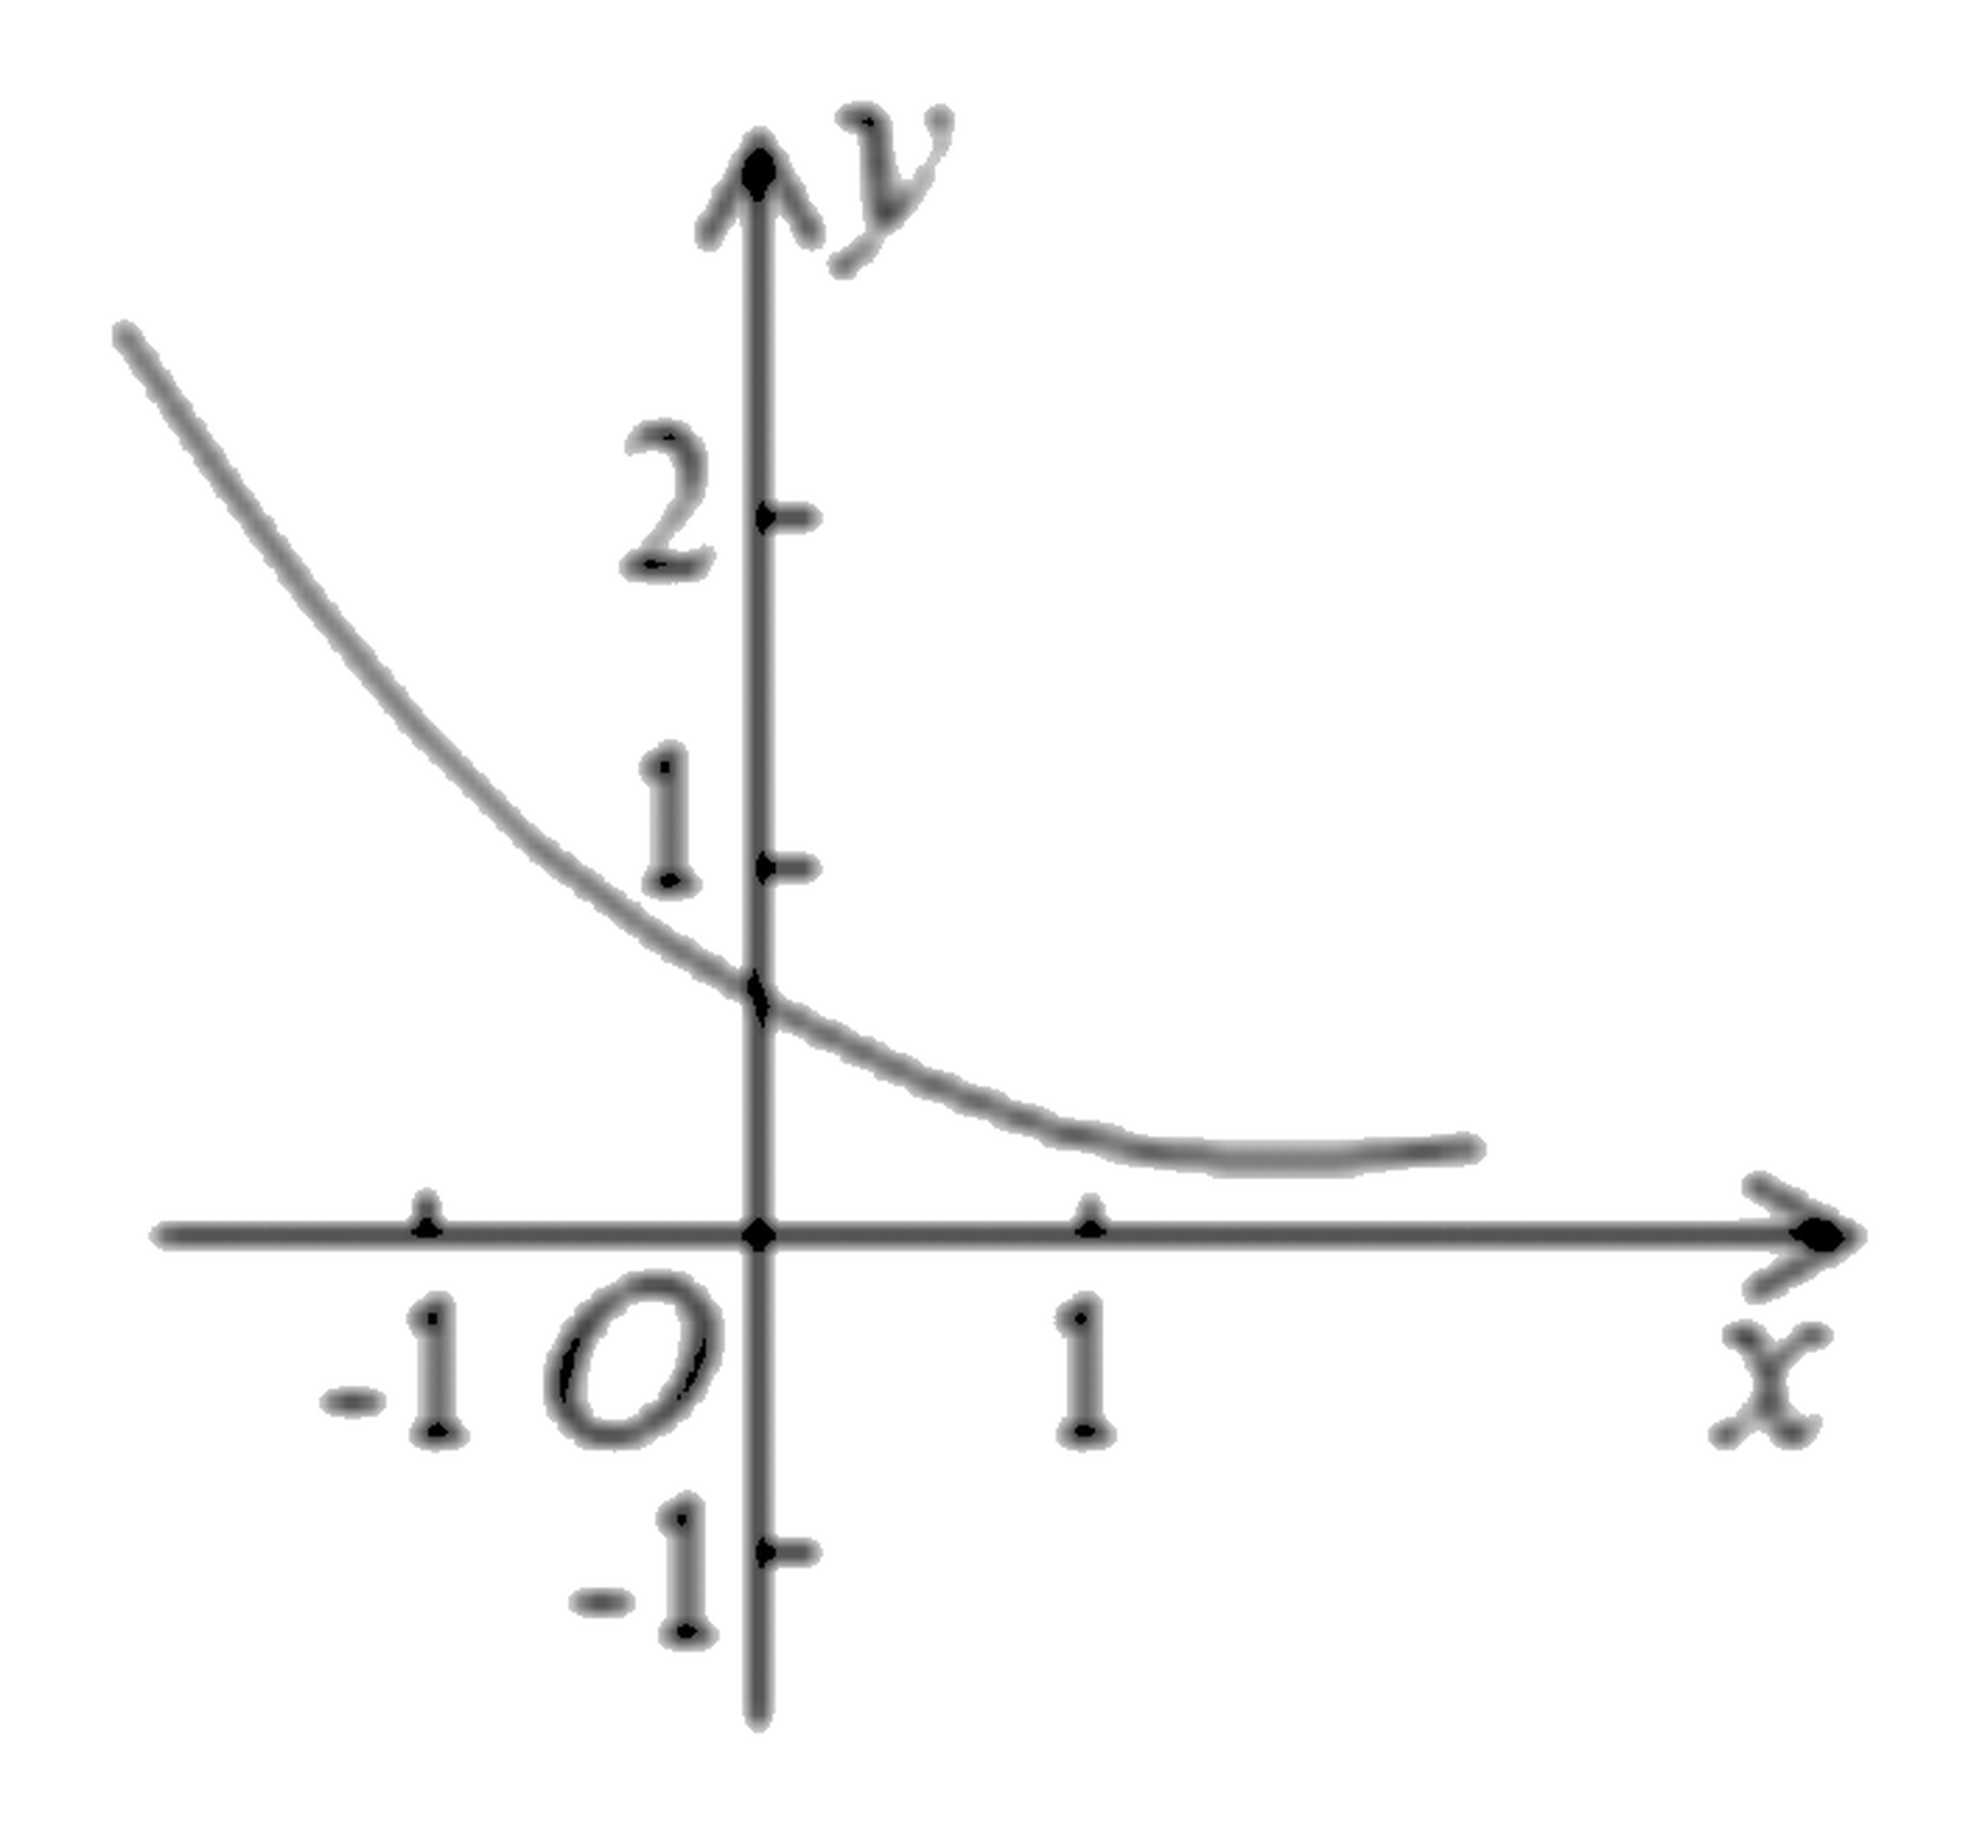
\includegraphics[width=0.30\textwidth]{figures/gao147_q15.png}
\end{center}

\ifanswer
\solbegin
\step{由图象从左到右下降得 $0<a<1$；}
\step{由图象与 $y$ 轴的交点得 $0<a^{-b}<1$，故 $b<0$；}
\step{故 $0<a<1$，$b<0$；故选 $D$.}
\solend
\fi

% === Q16 ===：位数新定义题（无弯引号，放大 04 页 z/q16_stem.png 确认）；四选项横排一行；解析 3 个印刷行
\item 数学运算是指在明晰运算对象的基础上，依据运算法则解决数学问题的素养. 因为运算，数的威力无限；没有运算，数就只是一个符号，对数运算与指数运算是两类重要的运算，对数的运算性质降低了运算的级别，简化了运算，在数学发展史上是伟大的成就. 而位数是指一个自然数有效位的个数，例如：$2^{10}=1024$，所以 $2^{10}$ 的位数为 4. 请你运用所学过的对数运算的知识，估计 $2025^{2026}$ 的位数是\mbox{（\quad）}

\keepwithprev
A. 6697\qquad B. 6698\qquad C. 6699\qquad D. 6700

\ifanswer
\solbegin
\step{设 $2025^{2026}=t$，所以 $\lg t=2026\lg2025$，}
\step{因为 $\lg2025\approx3.3064$，所以 $\lg t\approx6698.8$，}
\step{所以 $t\approx10^{6698.8}\in(10^{6698},10^{6699})$，所以 $2025^{2026}$ 的位数为 6699. 故选 $C$.}
\solend
\fi

\end{enumerate}

\bigsec{三、解答题}

\begin{enumerate}
\setcounter{enumi}{16}

% === Q17 ===：题干＋解析均在 04 页；集合描述竖线 \mid、描述内半角逗号照录；
% 空集 \varnothing、子集 \subseteq（放大 04 页 z/subset_04_q17b.png 确认带下划线）、数集 \R；
% 解析 5 个印刷行，首行末"所以 A=(-∞,-2)∪(3,+∞)"原卷无标点，照录不补
\item 已知集合 $A=\left\{x\mid \dfrac{x+2}{x-3}>0,x\in\R\right\}$，$B=\{x\mid \lvert x-2a\rvert\leqslant2,x\in\R\}$.

(1) 若 $a=1$，求 $A\cap B$；

(2) 若 $A\cap B=\varnothing$，求实数 $a$ 的取值范围.

\ifanswer
\solbegin
\step{由 $\dfrac{x+2}{x-3}>0$，得 $x<-2$ 或 $x>3$，所以 $A=(-\infty,-2)\cup(3,+\infty)$}
\step{(1) 当 $a=1$ 时，$B=\{x\mid \lvert x-2\rvert\leqslant2\}=[0,4]$，于是 $A\cap B=(3,4]$；}
\step{(2) $B=[2a-2,2a+2]$，}
\step{则 $A\cap B=\varnothing\Leftrightarrow[2a-2,2a+2]\subseteq[-2,3]\Leftrightarrow\begin{cases}2a-2\geqslant-2\\2a+2\leqslant3\end{cases}\Leftrightarrow0\leqslant a\leqslant\dfrac{1}{2}$，}
\step{所以实数 $a$ 的取值范围为 $\left[0,\dfrac{1}{2}\right]$.}
\solend
\fi

% === Q18 ===：氟化物／臭氧应用题；"氟化物""（如冰箱等）"全角夹注照录（放大 05 页 z/q18_line1.png 确认）；
% 关系式 $Q=Q_0e^{-0.0025t}$ 原卷独立一行，按一段照录；解析 6 个印刷行
\item 有些家用电器（如冰箱等）使用了氟化物，氟化物的释放破坏了大气上层的臭氧层，使臭氧含量 $Q$ 呈指数函数型变化，在氟化物排放量维持某种水平时，具有关系式

$Q=Q_0e^{-0.0025t}$，其中 $Q_0$ 是臭氧的初始量.

(1) 随时间 $t$ 的增加，臭氧的含量是增加还是减少？

(2) 试估计多少年以后将会有一半的臭氧消失.（用计算器计算）

\ifanswer
\solbegin
\step{(1) 对于函数 $Q=Q_0e^{-0.0025t}$，显然 $Q>0$，}
\step{任取 $t_1$、$t_2\in(0,+\infty)$，且 $t_1<t_2$，则 $t_2-t_1>0$，}
\step{所以 $\dfrac{Q_1}{Q_2}=\dfrac{Q_0e^{-0.0025t_1}}{Q_0e^{-0.0025t_2}}=e^{-0.0025(t_1-t_2)}=e^{0.0025(t_2-t_1)}>e^0=1$，所以 $Q_1>Q_2$，}
\step{故随着时间 $t$ 的增加，臭氧的含量是减少的；}
\step{(2) 令 $\dfrac{Q}{Q_0}=\dfrac{1}{2}$，即 $\dfrac{Q_0e^{-0.0025t}}{Q_0}=e^{-0.0025t}=\dfrac{1}{2}$，得 $-0.0025t=\ln\dfrac{1}{2}\approx-0.6931$，}
\step{解得 $t\approx277$，故估计 277 年以后将会有一半的臭氧消失.}
\solend
\fi

% === Q19 ===：题干用"图像"、解析两处用"图象"逐处照录不统一（05 页）；数集 \Z；
% 题干＋解析前 4 行在 05 页、解析后 3 行在 06 页；解析共 7 个印刷行
\item 已知幂函数 $f(x)=x^{-m^2+4m}(m\in\Z)$ 的图像关于 $y$ 轴对称，且在区间 $(0,+\infty)$ 上是严格增函数.

(1) 求 $m$ 的值；

(2) 求满足不等式 $(2a+1)^m<(a+1)^m$ 的实数 $a$ 的取值范围.

\ifanswer
\solbegin
\step{(1) 由题意得 $-m^2+4m>0$，解得 $0<m<4$，}
\step{因为 $m\in\Z$，所以 $m=1$ 或 $m=2$ 或 $m=3$.}
\step{当 $m=1$ 或 $m=3$ 时，$f(x)=x^3$，图象关于原点对称，不合题意；}
\step{当 $m=2$ 时，$f(x)=x^4$，图象关于 $y$ 轴对称，符合题意，所以 $m=2$.}
\step{(2) 代入 $m=2$，不等式为 $(2a+1)^2<(a+1)^2$，}
\step{得 $(2a+1)^2-(a+1)^2=a(3a+2)<0$，因此 $-\dfrac{2}{3}<a<0$，}
\step{所求范围为 $\left(-\dfrac{2}{3},0\right)$.}
\solend
\fi

% === Q20 ===：指数函数题，题干用"图像"；(3) 长求和式（分数 1/2026、1011/2026、2011/2026、
% 15/2026、1015/2026、2025/2026 放大 06 页 z/q20_sum_06a.png 确认）；题干在 06 页、
% 解析前 6 行在 06 页下半、后 6 行在 07 页上半；解析共 12 个印刷行
\item 已知指数函数 $y=a^x$（$a>0,a\ne1$）的图像经过点 $(1,4)$.

(1) 求实数 $a$ 的值；

(2) 若 $f(x)=(a^x)^2-2\cdot a^x-8$，当 $x\in\R$ 时，不等式 $f(x)>m\cdot4^x-12$ 恒成立，求 $m$ 的取值范围；

(3) 记 $g(x)=\dfrac{1}{a^x+2}$，求证：$g(x)+g(1-x)$ 为定值，并求 $g(0)+g\left(\dfrac{1}{2026}\right)+g\left(\dfrac{1011}{2026}\right)+g\left(\dfrac{2011}{2026}\right)+g\left(\dfrac{1}{2}\right)+g\left(\dfrac{15}{2026}\right)+g\left(\dfrac{1015}{2026}\right)+g\left(\dfrac{2025}{2026}\right)+g(1)$ 的值.

\ifanswer
\solbegin
\step{(1) 将 $(1,4)$ 代入 $y=a^x$，得 $a^1=4$，即 $a=4$.}
\step{(2) 令 $t=4^x$，当 $x\in\R$ 时，$t$ 取遍所有正实数.}
\step{原不等式等价于 $t^2-2t-8>mt-12\Leftrightarrow m<t+\dfrac{4}{t}-2$，}
\step{由基本不等式，$t+\dfrac{4}{t}-2\geqslant2\sqrt{t\cdot\dfrac{4}{t}}-2=2$，}
\step{当且仅当 $t=\dfrac{4}{t}$，即 $t=2$ 时取等号，}
\step{因此原不等式恒成立的充要条件为 $m<2$，即 $m\in(-\infty,2)$.}
\step{(3) 对任意 $x\in\R$，令 $t=4^x>0$，则 $4^{1-x}=\dfrac{4}{t}$，}
\step{从而 $g(x)+g(1-x)=\dfrac{1}{t+2}+\dfrac{1}{\dfrac{4}{t}+2}=\dfrac{1}{t+2}+\dfrac{t}{2(t+2)}=\dfrac{1}{2}$，}
\step{因此 $g(x)+g(1-x)$ 为定值 $\dfrac{1}{2}$.}
\step{原式中，0 与 1、$\dfrac{1}{2026}$ 与 $\dfrac{2025}{2026}$、$\dfrac{1011}{2026}$ 与 $\dfrac{1015}{2026}$、$\dfrac{2011}{2026}$ 与 $\dfrac{15}{2026}$}
\step{分别配对，每对函数值之和均为 $\dfrac{1}{2}$，且 $g\left(\dfrac{1}{2}\right)=\dfrac{1}{4^{\frac12}+2}=\dfrac{1}{4}$，}
\step{所以所求和为 $4\cdot\dfrac{1}{2}+\dfrac{1}{4}=\dfrac{9}{4}$.}
\solend
\fi

% === Q21 ===：不动点新定义题；题干在 07 页、解析续 08／09 页，共 20 个印刷行；
% 判别式两形混用：08 页 (2) cases 内等腰偏高 \Delta、09 页 (3) 扁等边 \triangle，逐处照录不统一
% （放大 /tmp/gao147/z/delta_vs_triangle.png 并排确认）；数集 \R；\forall 照录；
% 第 6—8 行是原卷一个长算式折成的三个印刷行，按印刷行分三条 \step、不并折行
\item 对于二次函数 $y=mx^2+nx+t(m\ne0)$，若存在 $x_0\in\R$，使得 $mx_0^2+nx_0+t=x_0$ 成立，则称 $x_0$ 为二次函数 $y=mx^2+nx+t(m\ne0)$ 的不动点.

(1) 求二次函数 $y=x^2-x-3$ 的不动点；

(2) 若二次函数 $y=2x^2-(3+a)x+a-1$ 有两个不相等的不动点 $x_1$、$x_2$，且 $x_1$、$x_2>0$，求 $\dfrac{x_1}{x_2}+\dfrac{x_2}{x_1}$ 的最小值；

(3) 若对任意实数 $b$，二次函数 $y=ax^2+(b+1)x+(b-1)(a\ne0)$ 恒有不动点，求 $a$ 的取值范围.

\ifanswer
\solbegin
\step{(1) 令 $x^2-x-3=x$，即 $x^2-2x-3=0$，即 $(x-3)(x+1)=0$，}
\step{解得 $x_1=-1$，$x_2=3$，所以不动点为 $-1$ 和 $3$.}
\step{(2) 由题意，$2x^2-(3+a)x+a-1=x$ 有两个不相等的正实数根，}
\step{即方程 $2x^2-(4+a)x+a-1=0$ 有两个不相等的正实数根，}
\step{所以 $\begin{cases}\Delta=(4+a)^2-8(a-1)>0\\x_1+x_2=\dfrac{4+a}{2}>0\\x_1\cdot x_2=\dfrac{a-1}{2}>0\end{cases}$，解得 $a>1$，}% 判别式原卷印等腰偏高粗三角 $\Delta$（放大 08 页 z/delta_08_q21cases.png）
\step{所以 $\dfrac{x_1}{x_2}+\dfrac{x_2}{x_1}=\dfrac{x_1^2+x_2^2}{x_1\cdot x_2}=\dfrac{(x_1+x_2)^2-2x_1\cdot x_2}{x_1\cdot x_2}=\dfrac{(x_1+x_2)^2}{x_1\cdot x_2}-2$}
\step{$=\dfrac{\left(\dfrac{4+a}{2}\right)^2}{\dfrac{a-1}{2}}-2=\dfrac{\dfrac{(a+4)^2}{4}}{\dfrac{a-1}{2}}-2=\dfrac{(a-1+5)^2}{2(a-1)}-2$}
\step{$=\dfrac{(a-1)^2+10(a-1)+25}{2(a-1)}-2=\dfrac{a-1}{2}+\dfrac{25}{2(a-1)}+3$.}
\step{因为 $a>1$，所以 $a-1>0$，}
\step{所以 $\dfrac{a-1}{2}+\dfrac{25}{2(a-1)}+3\geqslant2\sqrt{\dfrac{a-1}{2}\cdot\dfrac{25}{2(a-1)}}+3=8$，}
\step{当且仅当 $\dfrac{a-1}{2}=\dfrac{25}{2(a-1)}$，即 $a=6$ 时等号成立，}
\step{所以 $\dfrac{x_1}{x_2}+\dfrac{x_2}{x_1}$ 的最小值为 $8$.}
\step{(3) 设 $f(x)=ax^2+(b+1)x+b-1$，}
\step{则方程 $f(x)=x$，可化为 $ax^2+(b+1)x+b-1=x$，}
\step{即 $ax^2+bx+b-1=0$，}
\step{由题意得一元二次方程 $ax^2+bx+b-1=0$ 有解，又 $a\ne0$，}
\step{所以方程 $ax^2+bx+b-1=0$ 的判别式 $\triangle=b^2-4a(b-1)\geqslant0$，}% 判别式原卷印扁等边细线三角 $\triangle$（放大 09 页 z/triangle_09_q21.png），与 (2) 高 $\Delta$ 混用、照录不统一
\step{即 $b^2-4ab+4a\geqslant0$，则该不等式对 $\forall b\in\R$ 恒成立，}
\step{则 $(4a)^2-4\times4a\leqslant0$，且 $a\ne0$，解得 $0<a\leqslant1$，}
\step{所以实数 $a$ 的取值范围是 $(0,1]$.}
\solend
\fi

\end{enumerate}

\end{document}
"
%
% ① 原始材料：微信公众号"魔都数学加油站"文章，连载"27学年高一147"，原文标题
% "27学年高一147——2026-2027年上海市华师大三附中高一上期中"；
% 原文链接：https://mp.weixin.qq.com/s/X_gPW1JWoTAl2Bky_xEEGw 。
% 正文为 9 张 PNG 页（01/06/08/09 为 2560×3620，02/03/04/05/07 为 4762×6735，
% 同一篇各页分辨率混排，逐页按各自分辨率裁图核对，别按预览比例换算裁框）。
% 体例：混合体例讲评版——19 题中 Q4/Q5/Q7/Q9 只印【答案】、无【解析】，其余 15 题印
% 【解析】（逐题核实，见 ② ②）。题目、答案、解析均据原图转录；卷面粉红色水印
% "魔都数学加油站"及公众号页脚未录入。
% 全卷插图清单（逐页通读 9 页确认）：仅 1 处题目配图——
%   · Q15 递减指数函数小坐标系（03 页右侧：坐标轴、y 轴刻度 2/1/-1、x 轴刻度 -1/1、
%     原点 O、x/y 轴标），为"图像如图所示"的题目配图（选择题选项旁），三版都出；
%     裁自 03 页去粉色水印、去色、4× LANCZOS 放大存 figures/gao147_q15.png；
%   其余 8 页逐页确认无其它题目配图、无【解析】内配图、无表格，
%   亦无"题干写如图而源码漏图"一处；Q12/Q17/Q21 的 cases 块为数学块（非图）。
%
% 卷首标题：原卷印作"2026-2027 年华师大三附中高一上期中"，年份区间按全稿惯例排 en dash；
% 原卷卷面未印副标题，本稿按同期中卷（高一140／141／143／144／145／146）知识模块口径
% 补出"集合与常用逻辑用语、不等式、函数"。
%
% 题号体例（逐页核实定稿）：本卷共 19 题——一、填空题 3—12（10 题）、
% 二、选择题 13—16（4 题）、三、解答题 17—21（5 题）。
% 三节分别 \setcounter{enumi}{2}／{12}／{16}。原卷从第 3 题起、无第 1、2 题，
% 本稿保留原题号；全卷无附加题节（Q21 解析末行"所以实数 a 的取值范围是 (0,1]."
% 为全卷收尾，09 页下半仅水印、无正文）。
%
% ② 与原卷的排版差异：
%   ① 原文从第 3 题起，本稿保留原题号；共 19 题三节；
%   ② 混合体例：原卷 Q4/Q5/Q7/Q9 只印【答案】、无【解析】（分别为 a≤0、(-1,2)、
%      真、(-∞,1)），按 高一140 第 5 题／高一145 Q3 成例提 \ans{}、不补造解析；
%      其余 15 题印【解析】，用 \solbegin…\solend，选择题答案在解析末句"故选 X"
%      （Q13 选 B、Q14 选 B、Q15 选 D、Q16 选 C，逐个放大原图核实）、题干括号
%      \mbox{（\quad）} 留空、不另提 \ans{}；填空／解答答案落在解析里；
%      答案版【答案】/【解析】标记数 = 19（4 个 \ans ＋ 15 个 \solbegin）= 全卷题数；
%   ③ 原卷卷面未印副标题，本稿按知识模块口径补出；
%   ④ 原卷填空横线按全稿惯例排 \blankline[4.4em]；选择题括号排 \mbox{（\quad）}、
%      选项段前按惯例加 \keepwithprev；Q14／Q15 四选项为 2×2 两印刷行（A/B 一行、
%      C/D 一行），用空行分段照录（非一行 \qquad、亦非竖排四行）；解答题不留作答区、
%      不加 \anspace（原卷为讲评版，与 129／131／132／133／136／140／141／143／144／145／146 同）；
%   ⑤ 数集：Q4"A∪B=R"、Q13"f(x)=x^3 在 R 上严格增"、Q17"x∈R"两处、
%      Q20"x∈R"两处、Q21"x_0∈R""∀b∈R"原卷印斜体或黑板粗体 R，按全稿惯例统一改 \R；
%      Q19"m∈Z"改 \Z；本卷未出现 N（\N^* 无对应处）。绝对值排 \lvert…\rvert，
%      集合描述竖线排 \mid；不等号按全稿惯例排 \leqslant／\geqslant（原卷印 \le／\ge 形，
%      【答案】a≤0 亦排 \leqslant）；空集 \varnothing（Q17 两处）；
%      子集 \subseteq（Q17 带下划线，放大 04 页确认）；本卷未出现 \subset／\subsetneq，
%      亦未出现补集上划线 \overline{}；\left…\right 不得拆到不同 $…$ 组；
%   ⑥ 子题标号 (1)(2)(3) 半角括号照录；cases 块整体算一个印刷行（Q3、Q12 一行内
%      两个 cases、Q17、Q21(2)）；本卷解析内无圈数字①②③（无 \text{①} 需求）；
%      数学式内 CJK 用 \text{}（本卷未见）；
%   ⑦ 题干中的中文弯引号按原卷照录：Q7 命题"若 A∪B=B，则 A∩B=A"与
%      (填 " 真 " 或 " 假 ")、Q10 (填 ">" "<" "≤" "或≥")，含引号内空格；
%      注释内一律 ASCII 引号；Q16 位数新定义题逐字放大确认无弯引号
%      （交办提示的"Q16 新定义题"举例未在本卷出现），未补造引号；
%   ⑧ 半角逗号在数学组之间是全稿惯例、非笔误（Q4"$A=(-\infty,0],B=[a,+\infty)$"、
%      Q5"$(a>0,a\ne1)$"、Q17 集合描述内"$>0,x\in R$""$\leqslant2,x\in R$"、
%      Q20 题干"$(a>0,a\ne1)$"、Q21"$y=mx^2+nx+t(m\ne0)$"等），逐处照录别改全角；
%      行末西文句点照录为 ASCII `.`；行中全角逗号／顿号照录；
%      Q7／Q10"(填…)"为半角括号、Q18"（如冰箱等）"为全角括号，逐处照录不统一；
%   ⑨ "图像／图象"逐处照录不统一：题干 5 处用"图像"（Q5"图像恒过定点"、
%      Q9"图像位于直线 y=x 的下方"、Q15"的图像如图所示"、Q19"的图像关于 y 轴对称"、
%      Q20"的图像经过点"），解析 4 处用"图象"（Q15"由图象从左到右下降"
%      "由图象与 y 轴的交点"、Q19"图象关于原点对称""图象关于 y 轴对称"），逐处核、不统一；
%   ⑩ 判别式 Δ/△ 混用是照录项：Q21(2) 解析 cases 块"Δ=(4+a)²−8(a−1)>0"
%      印等腰偏高粗三角 \Delta，Q21(3) 解析"判别式△=b²−4a(b−1)≥0"
%      印扁等边细线三角 \triangle，逐处放大判断、照录不得统一
%      （参照 高一142／144／145 头注④口径，详见 ④）；
%   ⑪ 一条 \step = 原卷解析的一个印刷行，cases 块整体算一个印刷行；别把原卷折行
%      并起来、别把一行拆多条。Q10 七行（跨 01→02 页）、Q12 七行（含一行两 cases）、
%      Q20 十二行（含"原式中…2011/2026 与 15/2026／分别配对…"折行两行）、
%      Q21 二十行（含第 6—8 行一个长算式折成三印刷行、含 cases）均按印刷行逐条断，
%      不丢行；
%   ⑫ 配图：逐页通读 9 页确认全卷仅 Q15 一处题目配图（见 ①），三版都出、
%      \includegraphics[width=0.30\textwidth]；图块较小，未加 \needvspace 大图块守卫
%      （仅 \bigsec 自带 \needvspace{3\baselineskip}）；三版切页审计均"合计异常：无"；
%   ⑬ 跨页续印按题合并：Q3—Q9 在 01 页（Q10 题干在 01 页末、解析首行亦在 01 页末）；
%      Q10 解析续 02 页 6 行、Q11 在 02 页、Q12 题干＋解析前 4 行在 02 页
%      （解析续 03 页 3 行）；"二、选择题"标题与 Q13、Q14、Q15 题干＋解析前 2 行在 03 页
%      （Q15 配图在 03 页右侧）；Q15 解析末行与 Q16、"三、解答题"标题、Q17 在 04 页；
%      Q18 在 05 页、Q19 题干＋解析前 4 行在 05 页（解析续 06 页 3 行）；
%      Q20 题干＋解析前 6 行在 06 页（解析续 07 页 6 行）、Q21 题干＋解析前 3 行在 07 页；
%      Q21 解析续 08 页 13 行、续 09 页 4 行（09 页下半仅水印、无正文）。
%      本稿按题连排，不丢行、不并折行；
%   ⑭ 原卷解析内无红色"法一／法二"之类小标题，故本卷无 \stepm；
%      水印"魔都数学加油站"红色不录入。
%
% ③ 行数复核：一条 \step／\stepm = 原卷解析的一个印刷行，cases 块作一个印刷行计。
%   逐题数（主会话逐页核对定稿）：Q3：1；Q4：0（只印【答案】、提 \ans{}，不计入 \step 账）；
%   Q5：0；Q6：1；Q7：0；Q8：2；Q9：0；Q10：7；Q11：4；Q12：7；Q13：6；Q14：4；
%   Q15：3；Q16：3；Q17：5；Q18：6；Q19：7；Q20：12；Q21：20。
%   合计 88 条 \step（本卷无 \stepm：解析内无红色"法一／法二"类小标题），
%   与原卷逐题印刷行相等。全卷 15 题设 \solbegin…\solend ＋ 4 题一处 \ans{}，
%   答案版【答案】/【解析】标记数 = 19 = 全卷题数。
%
% ④ 判别式／子集符号结论（逐处放大原图照录、不得统一，主会话像素级复核）：
%   判别式全卷 2 处、两形混用逐处照录不统一（参照 高一142／144 头注④口径）：
%     · Q21(2) 解析 cases 块"Δ=(4+a)²−8(a−1)>0" 原卷印等腰偏高粗三角
%       （高>宽、粗笔画），照录 \Delta（放大 08 页 /tmp/gao147/z/delta_08_q21cases.png
%       与 z/delta_vs_triangle.png 左图确认）；
%     · Q21(3) 解析"判别式△=b²−4a(b−1)≥0" 原卷印扁等边细线三角
%       （宽≈高、细线），照录 \triangle（放大 09 页 /tmp/gao147/z/triangle_09_q21.png
%       与 z/delta_vs_triangle.png 右图并排确认）。
%   子集／补集：Q17 解析"[2a−2,2a+2]⊆[−2,3]" 原卷印带下划线 ⊆，照录 \subseteq
%     （放大 04 页 /tmp/gao147/z/subset_04_q17b.png 确认）；Q17"A∩B=∅"空集 \varnothing；
%     集合描述竖线 \mid（Q10 M、Q12 解集、Q17 A/B）；并集 \cup（Q4、Q17）、
%     交集 \cap（Q7、Q17）、不属于 \notin（Q10）；数集 \R／\Z 归一见 ② ⑤。
%   本卷未出现 \subset／\subsetneq，未出现补集上划线 \overline{}。
%
% ⑤ 存疑照录（放大原图确认，照录未改、正文对应处另有 % 注）：
%   1. Q4/Q5/Q7/Q9 只印【答案】、无【解析】，按成例提 \ans{}、不补造解析
%      （混合体例逐题核实，见 ② ②）。
%   2. Q21(2) 判别式高 \Delta 与 Q21(3) 判别式扁 \triangle 两形混用，
%      逐处照录不统一（见 ④）。
%   3. "图像／图象"题干 5 处"图像"、解析 4 处"图象"，逐处照录不统一（见 ② ⑨）。
%   4. Q7／Q10"(填…)"半角括号与 Q18"（如冰箱等）"全角括号，逐处照录不统一。
%   5. Q16 位数新定义题逐字放大确认无弯引号（交办提示的"Q16 新定义题"举例
%      未在本卷出现），未补造引号；全卷弯引号仅 Q7、Q10 两处。
%   6. Q17 解析首行末"所以 A=(-∞,-2)∪(3,+∞)"、Q20(3) 解析"…2011/2026 与 15/2026"
%      行末原卷均无标点，照录未补；Q21(2) 第 6—8 行一个长算式折成三印刷行，
%      按印刷行分三条 \step、不并折行。
%   全卷除此 6 类外未发现其它笔误／自相矛盾处。
%
% ⑥ 跨页续印按题合并说明：见 ② ⑬。
%
\documentclass[a4paper,11pt]{article}
\usepackage{common}

\begin{document}

\examtitlest[3]{2026--2027 年华师大三附中高一上期中}{集合与常用逻辑用语、不等式、函数}

\bigsec{一、填空题}

\begin{enumerate}
\setcounter{enumi}{2}

% === Q3 ===：印【解析】，1 个印刷行（cases 块整体算一行）
\item 函数 $y=(a^2-5a+7)a^x+6-2a$ 是指数函数，则 $a$ 的值为\blankline[4.4em].

\ifanswer
\solbegin
\step{由题意得 $\begin{cases}a^2-5a+7=1\\6-2a=0\end{cases}$，解得 $a=3$.}
\solend
\fi

% === Q4 ===：原卷只印【答案】、无【解析】，按 高一140 第 5 题／高一145 Q3 成例提 \ans{}、不补造解析；
% 题干数学组内半角逗号 $A=(-\infty,0],B=[a,+\infty)$ 照录（放大 01 页 z/q4_stem.png 确认）
\item 已知 $A=(-\infty,0],B=[a,+\infty)$，且 $A\cup B=\R$，则实数 $a$ 的取值范围为\blankline[4.4em].

\ifanswer
\ans{$a\leqslant0$}
\fi

% === Q5 ===：只印【答案】；题干"图像"照录（放大 01 页 z/q5_stem.png 确认）；
% 数学组内半角逗号 $(a>0,a\ne1)$ 照录
\item 函数 $y=a^{x+1}+1(a>0,a\ne1)$ 的图像恒过定点\blankline[4.4em].

\ifanswer
\ans{$(-1,2)$}
\fi

% === Q6 ===：印【解析】，1 个印刷行
\item 已知方程 $x^2+2x-4=0$ 的两个根为 $x_1$、$x_2$，则 $x_1^2+x_2^2$ 的值为\blankline[4.4em].

\ifanswer
\solbegin
\step{$x_1^2+x_2^2=(x_1+x_2)^2-2x_1x_2=4+8=12$.}
\solend
\fi

% === Q7 ===：只印【答案】；中文弯引号"若 A∪B=B，则 A∩B=A"与(填 " 真 " 或 " 假 ")内的空格照录
% （放大 01 页 z/q7_quotes_7x.png、z/q7_tail.png 确认，括号为半角）
\item 命题 “若 $A\cup B=B$，则 $A\cap B=A$” 为\blankline[4.4em]命题(填 “ 真 ” 或 “ 假 ”).

\ifanswer
\ans{真}
\fi

% === Q8 ===：印【解析】，2 个印刷行；不等号按全稿惯例 \geqslant／\leqslant
\item 已知正实数 $a$、$b$ 满足 $a+4b=1$，则 $ab$ 的最大值为\blankline[4.4em].

\ifanswer
\solbegin
\step{$a+4b\geqslant2\sqrt{a\cdot4b}\Rightarrow ab\leqslant\dfrac{1}{16}$，当且仅当 $a=4b=\dfrac{1}{2}$ 时取等号，}
\step{则 $ab$ 的最大值为 $\dfrac{1}{16}$.}
\solend
\fi

% === Q9 ===：只印【答案】；题干"图像"照录（放大 01 页 hi_01_2 确认）
\item 若幂函数 $y=x^s$ 在 $x>1$ 时的图像位于直线 $y=x$ 的下方，则 $s$ 的取值范围是\blankline[4.4em].

\ifanswer
\ans{$(-\infty,1)$}
\fi

% === Q10 ===：印【解析】，共 7 个印刷行（题在 01 页末起 1 行、续 02 页 6 行）；
% 题干跨两印刷行"则 |ab|+1 ____ |a|+|b|（填…）"按一句连排；(填…)为半角括号、引号内空格照录
\item 已知不等式 $\lvert2x+1\rvert+\lvert2x-1\rvert<4$ 的解集为 $M$. 设实数 $a\in M$，$b\notin M$，则 $\lvert ab\rvert+1$\blankline[4.4em] $\lvert a\rvert+\lvert b\rvert$(填 “$>$”，“$<$”，“$\leqslant$” “或$\geqslant$”).

\ifanswer
\solbegin
\step{当 $x<-\dfrac{1}{2}$ 时，不等式化为 $-2x-1+1-2x<4$，即 $x>-1$，所以 $-1<x<-\dfrac{1}{2}$；}
\step{当 $-\dfrac{1}{2}\leqslant x\leqslant\dfrac{1}{2}$ 时，不等式化为 $2x+1-2x+1<4$，即 $2<4$，所以 $-\dfrac{1}{2}\leqslant x\leqslant\dfrac{1}{2}$；}
\step{当 $x>\dfrac{1}{2}$ 时，不等式化为 $2x+1+2x-1<4$，即 $x<1$，所以 $\dfrac{1}{2}<x<1$；}
\step{综上，$M=\{x\mid -1<x<1\}$.}
\step{因为 $a\in M$，$b\notin M$，所以 $\lvert a\rvert<1$，$\lvert b\rvert\geqslant1$.}
\step{而 $\lvert ab\rvert+1-(\lvert a\rvert+\lvert b\rvert)=\lvert ab\rvert+1-\lvert a\rvert-\lvert b\rvert=(\lvert a\rvert-1)(\lvert b\rvert-1)$，}
\step{所以 $\lvert ab\rvert+1\leqslant\lvert a\rvert+\lvert b\rvert$.}
\solend
\fi

% === Q11 ===：印【解析】，4 个印刷行（02 页）
\item 已知 $m>1$，$n>1$，$\lg m=\log_n100$，则 $mn$ 的最小值为\blankline[4.4em].

\ifanswer
\solbegin
\step{由 $m>1$，$n>1$，得 $\lg m>0$，$\lg n>0$，}
\step{因为 $\lg m=\log_n100=\dfrac{\lg100}{\lg n}=\dfrac{2}{\lg n}$，所以 $\lg m\cdot\lg n=2$，}
\step{所以 $\lg(mn)=\lg m+\lg n\geqslant2\sqrt{\lg m\cdot\lg n}=2\sqrt2$，}
\step{当且仅当 $m=n=10^{\sqrt2}$ 时取等号，则 $mn\geqslant10^{2\sqrt2}$，即 $mn$ 的最小值为 $10^{2\sqrt2}$.}
\solend
\fi

% === Q12 ===：印【解析】，共 7 个印刷行（02 页 4 行、03 页 3 行）；
% 第 3 行"则 [cases]，得 [cases]，"两个 cases 块同属一个印刷行，整体作一条 \step（照 高一146 Q11 成例）
\item 已知关于 $x$ 的不等式 $ax^2+bx+c\leqslant1$ 的解集为 $\{x\mid -1\leqslant x\leqslant3\}$. 若关于 $x$ 的不等式 $ax^2+(b-1)x+c-2\leqslant0$ 有且仅有 8 个整数解，则实数 $a$ 的取值范围是\blankline[4.4em].

\ifanswer
\solbegin
\step{由已知关于 $x$ 的不等式 $ax^2+bx+c\leqslant1$ 的解集为 $\{x\mid -1\leqslant x\leqslant3\}$，}
\step{得 $a>0$，且方程 $ax^2+bx+c-1=0$ 的两根分别为 $-1$ 和 $3$，}
\step{则 $\begin{cases}-1+3=-\dfrac{b}{a}\\-1\times3=\dfrac{c-1}{a}\end{cases}$，得 $\begin{cases}b=-2a\\c=1-3a\end{cases}$，}
\step{不等式 $ax^2+(b-1)x+c-2\leqslant0$ 等价于 $ax^2-(2a+1)x-(3a+1)\leqslant0$，}
\step{即 $\left[x-\left(3+\dfrac{1}{a}\right)\right](x+1)\leqslant0$，解得 $-1\leqslant x\leqslant3+\dfrac{1}{a}$，}
\step{因为关于 $x$ 的不等式 $ax^2+(b-1)x+c-2\leqslant0$ 有且仅有 8 个整数解，}
\step{因此 $6\leqslant3+\dfrac{1}{a}<7$，即 $3\leqslant\dfrac{1}{a}<4$，解得 $\dfrac{1}{4}<a\leqslant\dfrac{1}{3}$，所以 $a$ 的取值范围为 $\left(\dfrac{1}{4},\dfrac{1}{3}\right]$.}
\solend
\fi

\end{enumerate}

\bigsec{二、选择题}

\begin{enumerate}
\setcounter{enumi}{12}

% === Q13 ===：题干＋选项＋解析均在 03 页；四选项横排一行；解析 6 个印刷行，末句"故选 B."
\item $a<b<0$，则下列不等式能成立的是\mbox{（\quad）}

\keepwithprev
A. $\dfrac{a}{b}<1$\qquad B. $\lvert a\rvert>-b$\qquad C. $\dfrac{1}{a}<\dfrac{1}{b}$\qquad D. $b^3<a^3$

\ifanswer
\solbegin
\step{对于 $A$，令 $a=-4$，$b=-3$，满足 $a<b<0$，但 $\dfrac{a}{b}>1$，故 $A$ 错误，}
\step{对于 $B$，因为 $a<b<0$，所以 $-a>-b>0$，即 $\lvert a\rvert>-b$，故 $B$ 正确，}
\step{对于 $C$，令 $a=-4$，$b=-3$，满足 $a<b<0$，但 $\dfrac{1}{a}>\dfrac{1}{b}$，故 $C$ 错误，}
\step{对于 $D$，$f(x)=x^3$ 在 $\R$ 上严格增，因为 $a<b$，所以 $f(a)<f(b)$，}
\step{即 $a^3<b^3$，故 $D$ 错误.}
\step{故选 $B$.}
\solend
\fi

% === Q14 ===：四选项原卷为 2×2 两印刷行（A/B 一行、C/D 一行），用空行分段照录；解析 4 个印刷行
\item 已知 $a$、$b$ 为实数，若 $\alpha:ab=0$，$\beta:a^2+\sqrt{b}=0$，则 $\alpha$ 是 $\beta$ 的\mbox{（\quad）}

\keepwithprev
A. 充分不必要条件\qquad\qquad B. 必要不充分条件

C. 充要条件\qquad\qquad D. 既不充分也不必要条件

\ifanswer
\solbegin
\step{$\beta:a^2+\sqrt{b}=0$，所以 $a=0$ 且 $b=0$，}
\step{由 $a=0$，$b=0\Rightarrow ab=0$，反之不成立.}
\step{所以 $ab=0$ 是 $a=0$，$b=0$ 的必要不充分条件，即 $\alpha$ 是 $\beta$ 的必要不充分条件，}
\step{故选 $B$.}
\solend
\fi

% === Q15 ===：题目配图（03 页右侧小坐标系），三版都出；题干用"图像"、解析用"图象"逐处照录；
% 四选项 2×2 两印刷行；解析 3 个印刷行（03 页 2 行、04 页 1 行，末句"故选 D."与前行同一印刷行）
\item 函数 $f(x)=a^{x-b}$ 的图像如图所示，其中 $a$、$b$ 为常数，则下列结论正确的是\mbox{（\quad）}

\keepwithprev
A. $a>1$，$b<0$\qquad\qquad B. $a>1$，$b>0$

C. $0<a<1$，$b>0$\qquad\qquad D. $0<a<1$，$b<0$

\begin{center}
% 递减指数函数小坐标系图取 03 页右侧，去粉色水印、去色、4× LANCZOS 放大；题目配图三版都出
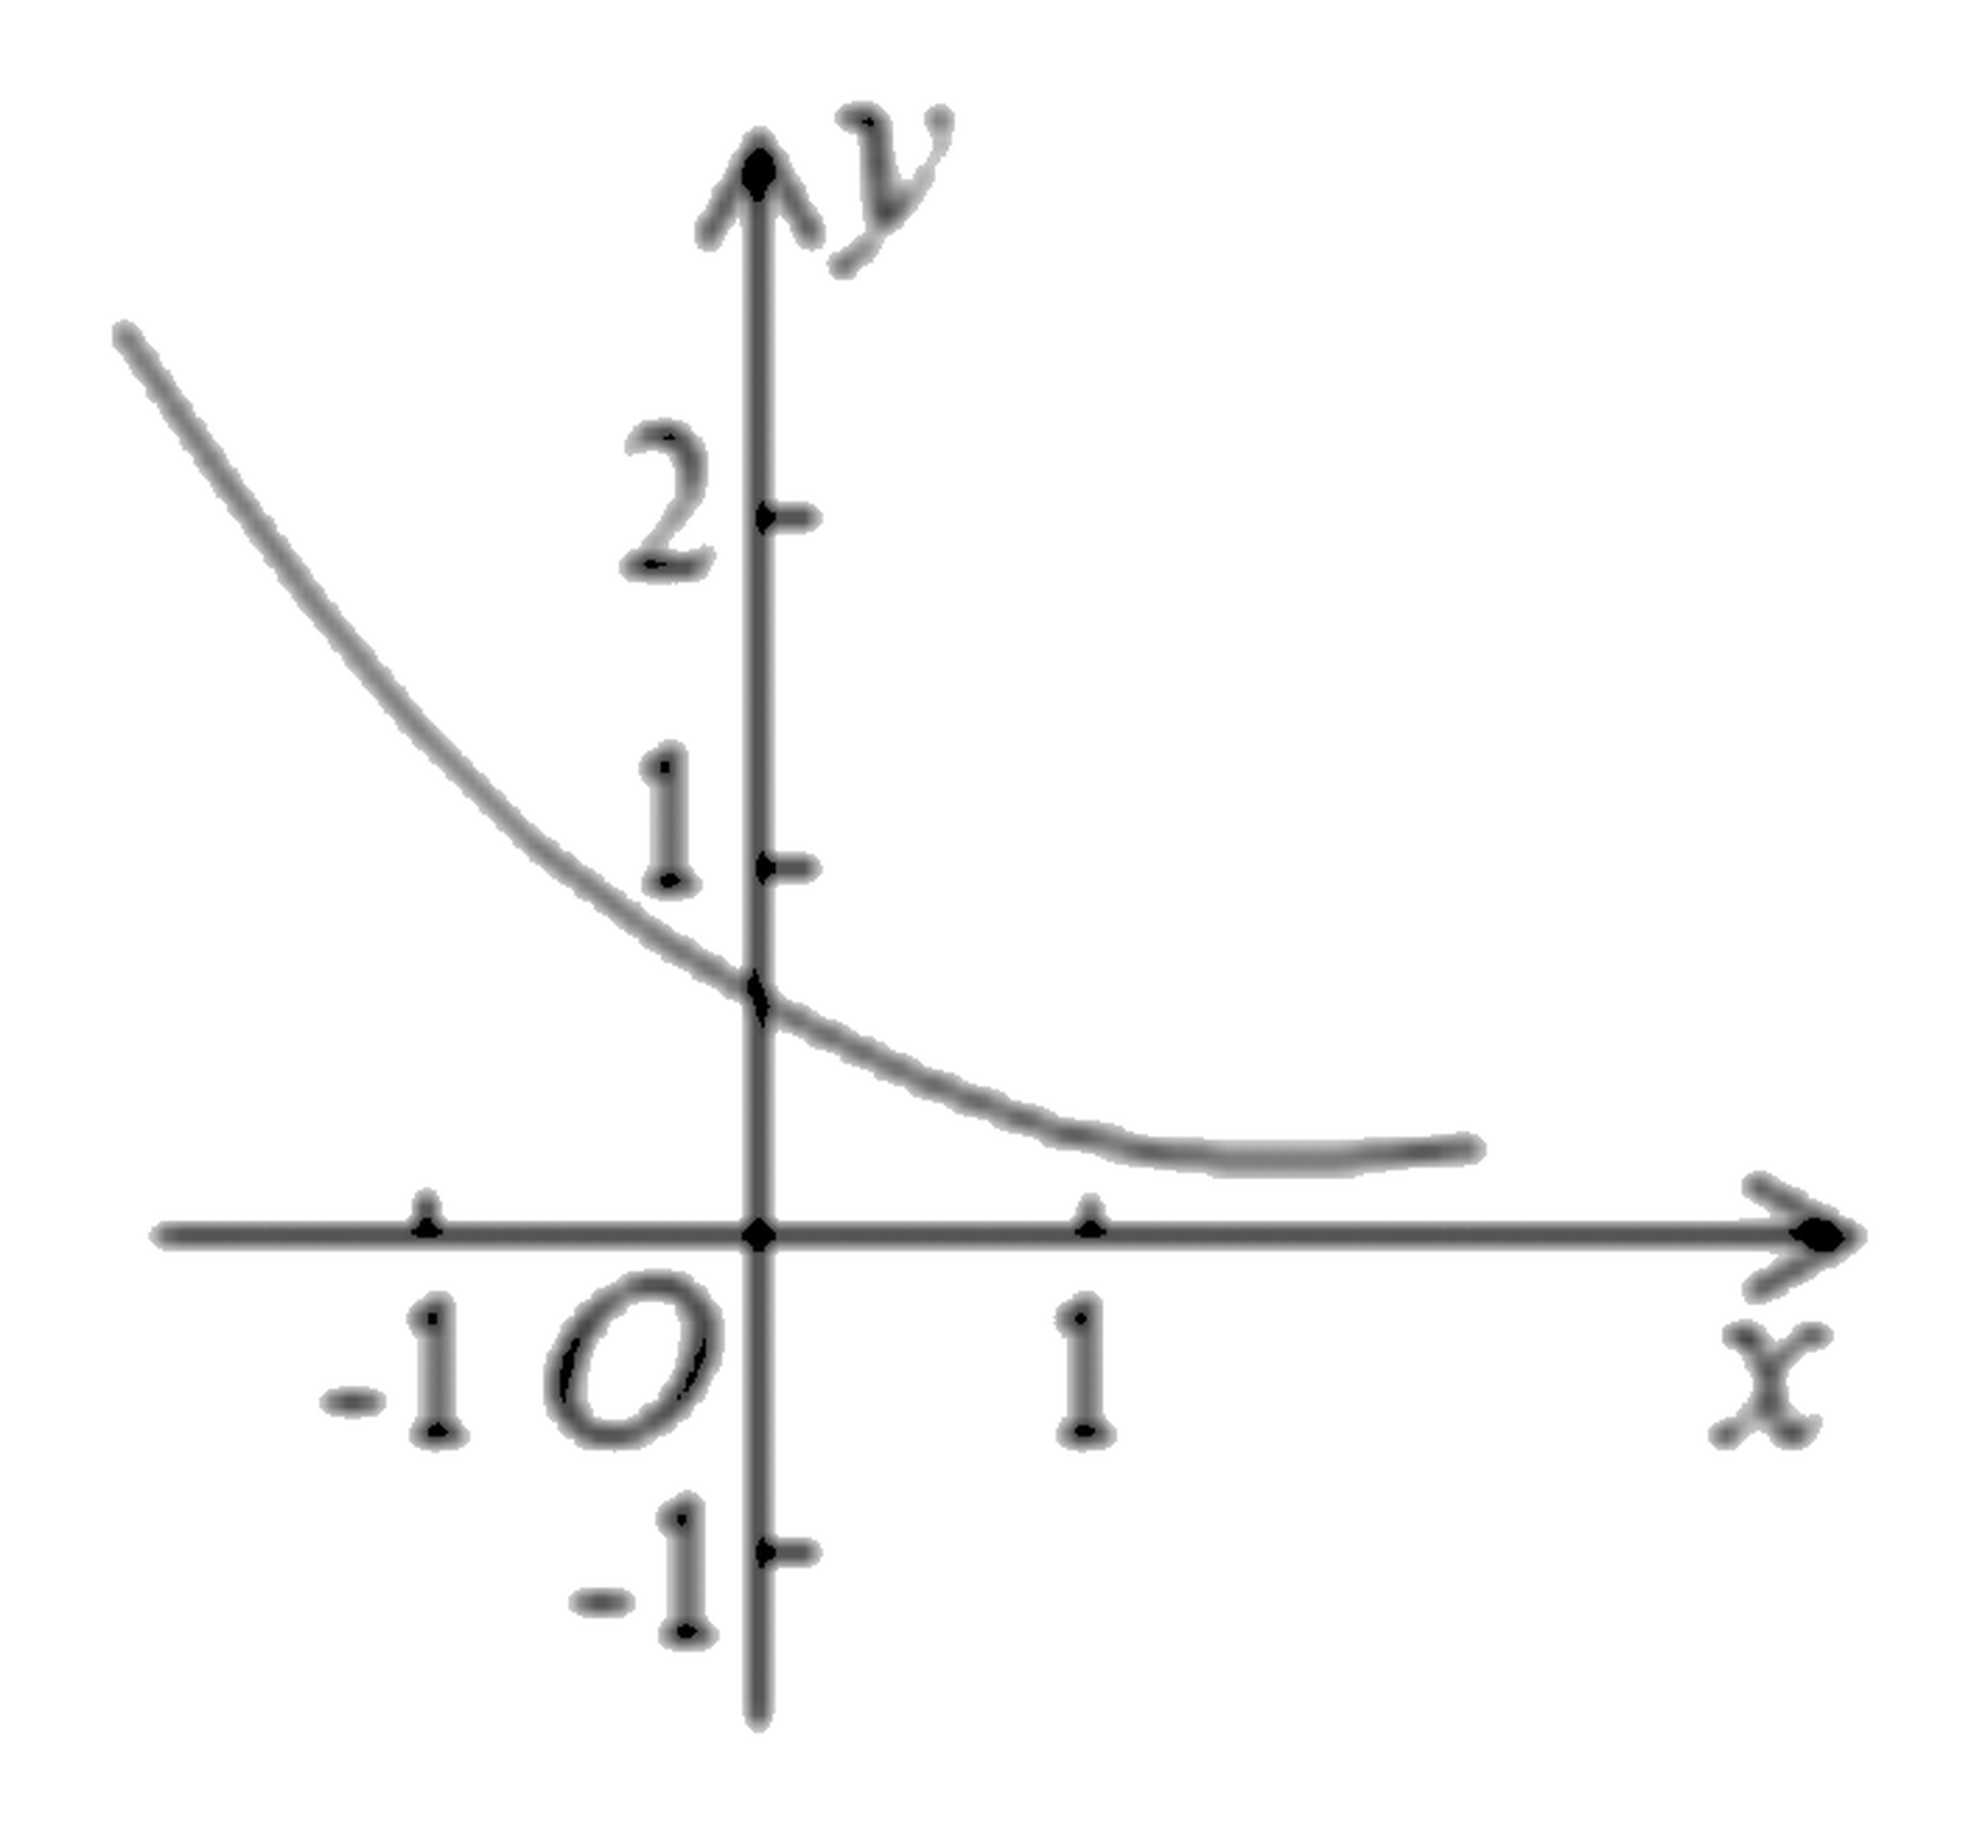
\includegraphics[width=0.30\textwidth]{figures/gao147_q15.png}
\end{center}

\ifanswer
\solbegin
\step{由图象从左到右下降得 $0<a<1$；}
\step{由图象与 $y$ 轴的交点得 $0<a^{-b}<1$，故 $b<0$；}
\step{故 $0<a<1$，$b<0$；故选 $D$.}
\solend
\fi

% === Q16 ===：位数新定义题（无弯引号，放大 04 页 z/q16_stem.png 确认）；四选项横排一行；解析 3 个印刷行
\item 数学运算是指在明晰运算对象的基础上，依据运算法则解决数学问题的素养. 因为运算，数的威力无限；没有运算，数就只是一个符号，对数运算与指数运算是两类重要的运算，对数的运算性质降低了运算的级别，简化了运算，在数学发展史上是伟大的成就. 而位数是指一个自然数有效位的个数，例如：$2^{10}=1024$，所以 $2^{10}$ 的位数为 4. 请你运用所学过的对数运算的知识，估计 $2025^{2026}$ 的位数是\mbox{（\quad）}

\keepwithprev
A. 6697\qquad B. 6698\qquad C. 6699\qquad D. 6700

\ifanswer
\solbegin
\step{设 $2025^{2026}=t$，所以 $\lg t=2026\lg2025$，}
\step{因为 $\lg2025\approx3.3064$，所以 $\lg t\approx6698.8$，}
\step{所以 $t\approx10^{6698.8}\in(10^{6698},10^{6699})$，所以 $2025^{2026}$ 的位数为 6699. 故选 $C$.}
\solend
\fi

\end{enumerate}

\bigsec{三、解答题}

\begin{enumerate}
\setcounter{enumi}{16}

% === Q17 ===：题干＋解析均在 04 页；集合描述竖线 \mid、描述内半角逗号照录；
% 空集 \varnothing、子集 \subseteq（放大 04 页 z/subset_04_q17b.png 确认带下划线）、数集 \R；
% 解析 5 个印刷行，首行末"所以 A=(-∞,-2)∪(3,+∞)"原卷无标点，照录不补
\item 已知集合 $A=\left\{x\mid \dfrac{x+2}{x-3}>0,x\in\R\right\}$，$B=\{x\mid \lvert x-2a\rvert\leqslant2,x\in\R\}$.

(1) 若 $a=1$，求 $A\cap B$；

(2) 若 $A\cap B=\varnothing$，求实数 $a$ 的取值范围.

\ifanswer
\solbegin
\step{由 $\dfrac{x+2}{x-3}>0$，得 $x<-2$ 或 $x>3$，所以 $A=(-\infty,-2)\cup(3,+\infty)$}
\step{(1) 当 $a=1$ 时，$B=\{x\mid \lvert x-2\rvert\leqslant2\}=[0,4]$，于是 $A\cap B=(3,4]$；}
\step{(2) $B=[2a-2,2a+2]$，}
\step{则 $A\cap B=\varnothing\Leftrightarrow[2a-2,2a+2]\subseteq[-2,3]\Leftrightarrow\begin{cases}2a-2\geqslant-2\\2a+2\leqslant3\end{cases}\Leftrightarrow0\leqslant a\leqslant\dfrac{1}{2}$，}
\step{所以实数 $a$ 的取值范围为 $\left[0,\dfrac{1}{2}\right]$.}
\solend
\fi

% === Q18 ===：氟化物／臭氧应用题；"氟化物""（如冰箱等）"全角夹注照录（放大 05 页 z/q18_line1.png 确认）；
% 关系式 $Q=Q_0e^{-0.0025t}$ 原卷独立一行，按一段照录；解析 6 个印刷行
\item 有些家用电器（如冰箱等）使用了氟化物，氟化物的释放破坏了大气上层的臭氧层，使臭氧含量 $Q$ 呈指数函数型变化，在氟化物排放量维持某种水平时，具有关系式

$Q=Q_0e^{-0.0025t}$，其中 $Q_0$ 是臭氧的初始量.

(1) 随时间 $t$ 的增加，臭氧的含量是增加还是减少？

(2) 试估计多少年以后将会有一半的臭氧消失.（用计算器计算）

\ifanswer
\solbegin
\step{(1) 对于函数 $Q=Q_0e^{-0.0025t}$，显然 $Q>0$，}
\step{任取 $t_1$、$t_2\in(0,+\infty)$，且 $t_1<t_2$，则 $t_2-t_1>0$，}
\step{所以 $\dfrac{Q_1}{Q_2}=\dfrac{Q_0e^{-0.0025t_1}}{Q_0e^{-0.0025t_2}}=e^{-0.0025(t_1-t_2)}=e^{0.0025(t_2-t_1)}>e^0=1$，所以 $Q_1>Q_2$，}
\step{故随着时间 $t$ 的增加，臭氧的含量是减少的；}
\step{(2) 令 $\dfrac{Q}{Q_0}=\dfrac{1}{2}$，即 $\dfrac{Q_0e^{-0.0025t}}{Q_0}=e^{-0.0025t}=\dfrac{1}{2}$，得 $-0.0025t=\ln\dfrac{1}{2}\approx-0.6931$，}
\step{解得 $t\approx277$，故估计 277 年以后将会有一半的臭氧消失.}
\solend
\fi

% === Q19 ===：题干用"图像"、解析两处用"图象"逐处照录不统一（05 页）；数集 \Z；
% 题干＋解析前 4 行在 05 页、解析后 3 行在 06 页；解析共 7 个印刷行
\item 已知幂函数 $f(x)=x^{-m^2+4m}(m\in\Z)$ 的图像关于 $y$ 轴对称，且在区间 $(0,+\infty)$ 上是严格增函数.

(1) 求 $m$ 的值；

(2) 求满足不等式 $(2a+1)^m<(a+1)^m$ 的实数 $a$ 的取值范围.

\ifanswer
\solbegin
\step{(1) 由题意得 $-m^2+4m>0$，解得 $0<m<4$，}
\step{因为 $m\in\Z$，所以 $m=1$ 或 $m=2$ 或 $m=3$.}
\step{当 $m=1$ 或 $m=3$ 时，$f(x)=x^3$，图象关于原点对称，不合题意；}
\step{当 $m=2$ 时，$f(x)=x^4$，图象关于 $y$ 轴对称，符合题意，所以 $m=2$.}
\step{(2) 代入 $m=2$，不等式为 $(2a+1)^2<(a+1)^2$，}
\step{得 $(2a+1)^2-(a+1)^2=a(3a+2)<0$，因此 $-\dfrac{2}{3}<a<0$，}
\step{所求范围为 $\left(-\dfrac{2}{3},0\right)$.}
\solend
\fi

% === Q20 ===：指数函数题，题干用"图像"；(3) 长求和式（分数 1/2026、1011/2026、2011/2026、
% 15/2026、1015/2026、2025/2026 放大 06 页 z/q20_sum_06a.png 确认）；题干在 06 页、
% 解析前 6 行在 06 页下半、后 6 行在 07 页上半；解析共 12 个印刷行
\item 已知指数函数 $y=a^x$（$a>0,a\ne1$）的图像经过点 $(1,4)$.

(1) 求实数 $a$ 的值；

(2) 若 $f(x)=(a^x)^2-2\cdot a^x-8$，当 $x\in\R$ 时，不等式 $f(x)>m\cdot4^x-12$ 恒成立，求 $m$ 的取值范围；

(3) 记 $g(x)=\dfrac{1}{a^x+2}$，求证：$g(x)+g(1-x)$ 为定值，并求 $g(0)+g\left(\dfrac{1}{2026}\right)+g\left(\dfrac{1011}{2026}\right)+g\left(\dfrac{2011}{2026}\right)+g\left(\dfrac{1}{2}\right)+g\left(\dfrac{15}{2026}\right)+g\left(\dfrac{1015}{2026}\right)+g\left(\dfrac{2025}{2026}\right)+g(1)$ 的值.

\ifanswer
\solbegin
\step{(1) 将 $(1,4)$ 代入 $y=a^x$，得 $a^1=4$，即 $a=4$.}
\step{(2) 令 $t=4^x$，当 $x\in\R$ 时，$t$ 取遍所有正实数.}
\step{原不等式等价于 $t^2-2t-8>mt-12\Leftrightarrow m<t+\dfrac{4}{t}-2$，}
\step{由基本不等式，$t+\dfrac{4}{t}-2\geqslant2\sqrt{t\cdot\dfrac{4}{t}}-2=2$，}
\step{当且仅当 $t=\dfrac{4}{t}$，即 $t=2$ 时取等号，}
\step{因此原不等式恒成立的充要条件为 $m<2$，即 $m\in(-\infty,2)$.}
\step{(3) 对任意 $x\in\R$，令 $t=4^x>0$，则 $4^{1-x}=\dfrac{4}{t}$，}
\step{从而 $g(x)+g(1-x)=\dfrac{1}{t+2}+\dfrac{1}{\dfrac{4}{t}+2}=\dfrac{1}{t+2}+\dfrac{t}{2(t+2)}=\dfrac{1}{2}$，}
\step{因此 $g(x)+g(1-x)$ 为定值 $\dfrac{1}{2}$.}
\step{原式中，0 与 1、$\dfrac{1}{2026}$ 与 $\dfrac{2025}{2026}$、$\dfrac{1011}{2026}$ 与 $\dfrac{1015}{2026}$、$\dfrac{2011}{2026}$ 与 $\dfrac{15}{2026}$}
\step{分别配对，每对函数值之和均为 $\dfrac{1}{2}$，且 $g\left(\dfrac{1}{2}\right)=\dfrac{1}{4^{\frac12}+2}=\dfrac{1}{4}$，}
\step{所以所求和为 $4\cdot\dfrac{1}{2}+\dfrac{1}{4}=\dfrac{9}{4}$.}
\solend
\fi

% === Q21 ===：不动点新定义题；题干在 07 页、解析续 08／09 页，共 20 个印刷行；
% 判别式两形混用：08 页 (2) cases 内等腰偏高 \Delta、09 页 (3) 扁等边 \triangle，逐处照录不统一
% （放大 /tmp/gao147/z/delta_vs_triangle.png 并排确认）；数集 \R；\forall 照录；
% 第 6—8 行是原卷一个长算式折成的三个印刷行，按印刷行分三条 \step、不并折行
\item 对于二次函数 $y=mx^2+nx+t(m\ne0)$，若存在 $x_0\in\R$，使得 $mx_0^2+nx_0+t=x_0$ 成立，则称 $x_0$ 为二次函数 $y=mx^2+nx+t(m\ne0)$ 的不动点.

(1) 求二次函数 $y=x^2-x-3$ 的不动点；

(2) 若二次函数 $y=2x^2-(3+a)x+a-1$ 有两个不相等的不动点 $x_1$、$x_2$，且 $x_1$、$x_2>0$，求 $\dfrac{x_1}{x_2}+\dfrac{x_2}{x_1}$ 的最小值；

(3) 若对任意实数 $b$，二次函数 $y=ax^2+(b+1)x+(b-1)(a\ne0)$ 恒有不动点，求 $a$ 的取值范围.

\ifanswer
\solbegin
\step{(1) 令 $x^2-x-3=x$，即 $x^2-2x-3=0$，即 $(x-3)(x+1)=0$，}
\step{解得 $x_1=-1$，$x_2=3$，所以不动点为 $-1$ 和 $3$.}
\step{(2) 由题意，$2x^2-(3+a)x+a-1=x$ 有两个不相等的正实数根，}
\step{即方程 $2x^2-(4+a)x+a-1=0$ 有两个不相等的正实数根，}
\step{所以 $\begin{cases}\Delta=(4+a)^2-8(a-1)>0\\x_1+x_2=\dfrac{4+a}{2}>0\\x_1\cdot x_2=\dfrac{a-1}{2}>0\end{cases}$，解得 $a>1$，}% 判别式原卷印等腰偏高粗三角 $\Delta$（放大 08 页 z/delta_08_q21cases.png）
\step{所以 $\dfrac{x_1}{x_2}+\dfrac{x_2}{x_1}=\dfrac{x_1^2+x_2^2}{x_1\cdot x_2}=\dfrac{(x_1+x_2)^2-2x_1\cdot x_2}{x_1\cdot x_2}=\dfrac{(x_1+x_2)^2}{x_1\cdot x_2}-2$}
\step{$=\dfrac{\left(\dfrac{4+a}{2}\right)^2}{\dfrac{a-1}{2}}-2=\dfrac{\dfrac{(a+4)^2}{4}}{\dfrac{a-1}{2}}-2=\dfrac{(a-1+5)^2}{2(a-1)}-2$}
\step{$=\dfrac{(a-1)^2+10(a-1)+25}{2(a-1)}-2=\dfrac{a-1}{2}+\dfrac{25}{2(a-1)}+3$.}
\step{因为 $a>1$，所以 $a-1>0$，}
\step{所以 $\dfrac{a-1}{2}+\dfrac{25}{2(a-1)}+3\geqslant2\sqrt{\dfrac{a-1}{2}\cdot\dfrac{25}{2(a-1)}}+3=8$，}
\step{当且仅当 $\dfrac{a-1}{2}=\dfrac{25}{2(a-1)}$，即 $a=6$ 时等号成立，}
\step{所以 $\dfrac{x_1}{x_2}+\dfrac{x_2}{x_1}$ 的最小值为 $8$.}
\step{(3) 设 $f(x)=ax^2+(b+1)x+b-1$，}
\step{则方程 $f(x)=x$，可化为 $ax^2+(b+1)x+b-1=x$，}
\step{即 $ax^2+bx+b-1=0$，}
\step{由题意得一元二次方程 $ax^2+bx+b-1=0$ 有解，又 $a\ne0$，}
\step{所以方程 $ax^2+bx+b-1=0$ 的判别式 $\triangle=b^2-4a(b-1)\geqslant0$，}% 判别式原卷印扁等边细线三角 $\triangle$（放大 09 页 z/triangle_09_q21.png），与 (2) 高 $\Delta$ 混用、照录不统一
\step{即 $b^2-4ab+4a\geqslant0$，则该不等式对 $\forall b\in\R$ 恒成立，}
\step{则 $(4a)^2-4\times4a\leqslant0$，且 $a\ne0$，解得 $0<a\leqslant1$，}
\step{所以实数 $a$ 的取值范围是 $(0,1]$.}
\solend
\fi

\end{enumerate}

\end{document}
"
% 紧凑版：xelatex "\def\iscompact{1}% 高一147_华师大三附中_期中.tex
%   —— 高一上数学"2026-2027 年华师大三附中高一上期中"（试卷版/答案版/紧凑版）
% 试卷版：xelatex 高一147_华师大三附中_期中.tex
% 答案版：xelatex "\def\isanswer{1}% 高一147_华师大三附中_期中.tex
%   —— 高一上数学"2026-2027 年华师大三附中高一上期中"（试卷版/答案版/紧凑版）
% 试卷版：xelatex 高一147_华师大三附中_期中.tex
% 答案版：xelatex "\def\isanswer{1}% 高一147_华师大三附中_期中.tex
%   —— 高一上数学"2026-2027 年华师大三附中高一上期中"（试卷版/答案版/紧凑版）
% 试卷版：xelatex 高一147_华师大三附中_期中.tex
% 答案版：xelatex "\def\isanswer{1}\input{高一147_华师大三附中_期中.tex}"
% 紧凑版：xelatex "\def\iscompact{1}\input{高一147_华师大三附中_期中.tex}"
%
% ① 原始材料：微信公众号"魔都数学加油站"文章，连载"27学年高一147"，原文标题
% "27学年高一147——2026-2027年上海市华师大三附中高一上期中"；
% 原文链接：https://mp.weixin.qq.com/s/X_gPW1JWoTAl2Bky_xEEGw 。
% 正文为 9 张 PNG 页（01/06/08/09 为 2560×3620，02/03/04/05/07 为 4762×6735，
% 同一篇各页分辨率混排，逐页按各自分辨率裁图核对，别按预览比例换算裁框）。
% 体例：混合体例讲评版——19 题中 Q4/Q5/Q7/Q9 只印【答案】、无【解析】，其余 15 题印
% 【解析】（逐题核实，见 ② ②）。题目、答案、解析均据原图转录；卷面粉红色水印
% "魔都数学加油站"及公众号页脚未录入。
% 全卷插图清单（逐页通读 9 页确认）：仅 1 处题目配图——
%   · Q15 递减指数函数小坐标系（03 页右侧：坐标轴、y 轴刻度 2/1/-1、x 轴刻度 -1/1、
%     原点 O、x/y 轴标），为"图像如图所示"的题目配图（选择题选项旁），三版都出；
%     裁自 03 页去粉色水印、去色、4× LANCZOS 放大存 figures/gao147_q15.png；
%   其余 8 页逐页确认无其它题目配图、无【解析】内配图、无表格，
%   亦无"题干写如图而源码漏图"一处；Q12/Q17/Q21 的 cases 块为数学块（非图）。
%
% 卷首标题：原卷印作"2026-2027 年华师大三附中高一上期中"，年份区间按全稿惯例排 en dash；
% 原卷卷面未印副标题，本稿按同期中卷（高一140／141／143／144／145／146）知识模块口径
% 补出"集合与常用逻辑用语、不等式、函数"。
%
% 题号体例（逐页核实定稿）：本卷共 19 题——一、填空题 3—12（10 题）、
% 二、选择题 13—16（4 题）、三、解答题 17—21（5 题）。
% 三节分别 \setcounter{enumi}{2}／{12}／{16}。原卷从第 3 题起、无第 1、2 题，
% 本稿保留原题号；全卷无附加题节（Q21 解析末行"所以实数 a 的取值范围是 (0,1]."
% 为全卷收尾，09 页下半仅水印、无正文）。
%
% ② 与原卷的排版差异：
%   ① 原文从第 3 题起，本稿保留原题号；共 19 题三节；
%   ② 混合体例：原卷 Q4/Q5/Q7/Q9 只印【答案】、无【解析】（分别为 a≤0、(-1,2)、
%      真、(-∞,1)），按 高一140 第 5 题／高一145 Q3 成例提 \ans{}、不补造解析；
%      其余 15 题印【解析】，用 \solbegin…\solend，选择题答案在解析末句"故选 X"
%      （Q13 选 B、Q14 选 B、Q15 选 D、Q16 选 C，逐个放大原图核实）、题干括号
%      \mbox{（\quad）} 留空、不另提 \ans{}；填空／解答答案落在解析里；
%      答案版【答案】/【解析】标记数 = 19（4 个 \ans ＋ 15 个 \solbegin）= 全卷题数；
%   ③ 原卷卷面未印副标题，本稿按知识模块口径补出；
%   ④ 原卷填空横线按全稿惯例排 \blankline[4.4em]；选择题括号排 \mbox{（\quad）}、
%      选项段前按惯例加 \keepwithprev；Q14／Q15 四选项为 2×2 两印刷行（A/B 一行、
%      C/D 一行），用空行分段照录（非一行 \qquad、亦非竖排四行）；解答题不留作答区、
%      不加 \anspace（原卷为讲评版，与 129／131／132／133／136／140／141／143／144／145／146 同）；
%   ⑤ 数集：Q4"A∪B=R"、Q13"f(x)=x^3 在 R 上严格增"、Q17"x∈R"两处、
%      Q20"x∈R"两处、Q21"x_0∈R""∀b∈R"原卷印斜体或黑板粗体 R，按全稿惯例统一改 \R；
%      Q19"m∈Z"改 \Z；本卷未出现 N（\N^* 无对应处）。绝对值排 \lvert…\rvert，
%      集合描述竖线排 \mid；不等号按全稿惯例排 \leqslant／\geqslant（原卷印 \le／\ge 形，
%      【答案】a≤0 亦排 \leqslant）；空集 \varnothing（Q17 两处）；
%      子集 \subseteq（Q17 带下划线，放大 04 页确认）；本卷未出现 \subset／\subsetneq，
%      亦未出现补集上划线 \overline{}；\left…\right 不得拆到不同 $…$ 组；
%   ⑥ 子题标号 (1)(2)(3) 半角括号照录；cases 块整体算一个印刷行（Q3、Q12 一行内
%      两个 cases、Q17、Q21(2)）；本卷解析内无圈数字①②③（无 \text{①} 需求）；
%      数学式内 CJK 用 \text{}（本卷未见）；
%   ⑦ 题干中的中文弯引号按原卷照录：Q7 命题"若 A∪B=B，则 A∩B=A"与
%      (填 " 真 " 或 " 假 ")、Q10 (填 ">" "<" "≤" "或≥")，含引号内空格；
%      注释内一律 ASCII 引号；Q16 位数新定义题逐字放大确认无弯引号
%      （交办提示的"Q16 新定义题"举例未在本卷出现），未补造引号；
%   ⑧ 半角逗号在数学组之间是全稿惯例、非笔误（Q4"$A=(-\infty,0],B=[a,+\infty)$"、
%      Q5"$(a>0,a\ne1)$"、Q17 集合描述内"$>0,x\in R$""$\leqslant2,x\in R$"、
%      Q20 题干"$(a>0,a\ne1)$"、Q21"$y=mx^2+nx+t(m\ne0)$"等），逐处照录别改全角；
%      行末西文句点照录为 ASCII `.`；行中全角逗号／顿号照录；
%      Q7／Q10"(填…)"为半角括号、Q18"（如冰箱等）"为全角括号，逐处照录不统一；
%   ⑨ "图像／图象"逐处照录不统一：题干 5 处用"图像"（Q5"图像恒过定点"、
%      Q9"图像位于直线 y=x 的下方"、Q15"的图像如图所示"、Q19"的图像关于 y 轴对称"、
%      Q20"的图像经过点"），解析 4 处用"图象"（Q15"由图象从左到右下降"
%      "由图象与 y 轴的交点"、Q19"图象关于原点对称""图象关于 y 轴对称"），逐处核、不统一；
%   ⑩ 判别式 Δ/△ 混用是照录项：Q21(2) 解析 cases 块"Δ=(4+a)²−8(a−1)>0"
%      印等腰偏高粗三角 \Delta，Q21(3) 解析"判别式△=b²−4a(b−1)≥0"
%      印扁等边细线三角 \triangle，逐处放大判断、照录不得统一
%      （参照 高一142／144／145 头注④口径，详见 ④）；
%   ⑪ 一条 \step = 原卷解析的一个印刷行，cases 块整体算一个印刷行；别把原卷折行
%      并起来、别把一行拆多条。Q10 七行（跨 01→02 页）、Q12 七行（含一行两 cases）、
%      Q20 十二行（含"原式中…2011/2026 与 15/2026／分别配对…"折行两行）、
%      Q21 二十行（含第 6—8 行一个长算式折成三印刷行、含 cases）均按印刷行逐条断，
%      不丢行；
%   ⑫ 配图：逐页通读 9 页确认全卷仅 Q15 一处题目配图（见 ①），三版都出、
%      \includegraphics[width=0.30\textwidth]；图块较小，未加 \needvspace 大图块守卫
%      （仅 \bigsec 自带 \needvspace{3\baselineskip}）；三版切页审计均"合计异常：无"；
%   ⑬ 跨页续印按题合并：Q3—Q9 在 01 页（Q10 题干在 01 页末、解析首行亦在 01 页末）；
%      Q10 解析续 02 页 6 行、Q11 在 02 页、Q12 题干＋解析前 4 行在 02 页
%      （解析续 03 页 3 行）；"二、选择题"标题与 Q13、Q14、Q15 题干＋解析前 2 行在 03 页
%      （Q15 配图在 03 页右侧）；Q15 解析末行与 Q16、"三、解答题"标题、Q17 在 04 页；
%      Q18 在 05 页、Q19 题干＋解析前 4 行在 05 页（解析续 06 页 3 行）；
%      Q20 题干＋解析前 6 行在 06 页（解析续 07 页 6 行）、Q21 题干＋解析前 3 行在 07 页；
%      Q21 解析续 08 页 13 行、续 09 页 4 行（09 页下半仅水印、无正文）。
%      本稿按题连排，不丢行、不并折行；
%   ⑭ 原卷解析内无红色"法一／法二"之类小标题，故本卷无 \stepm；
%      水印"魔都数学加油站"红色不录入。
%
% ③ 行数复核：一条 \step／\stepm = 原卷解析的一个印刷行，cases 块作一个印刷行计。
%   逐题数（主会话逐页核对定稿）：Q3：1；Q4：0（只印【答案】、提 \ans{}，不计入 \step 账）；
%   Q5：0；Q6：1；Q7：0；Q8：2；Q9：0；Q10：7；Q11：4；Q12：7；Q13：6；Q14：4；
%   Q15：3；Q16：3；Q17：5；Q18：6；Q19：7；Q20：12；Q21：20。
%   合计 88 条 \step（本卷无 \stepm：解析内无红色"法一／法二"类小标题），
%   与原卷逐题印刷行相等。全卷 15 题设 \solbegin…\solend ＋ 4 题一处 \ans{}，
%   答案版【答案】/【解析】标记数 = 19 = 全卷题数。
%
% ④ 判别式／子集符号结论（逐处放大原图照录、不得统一，主会话像素级复核）：
%   判别式全卷 2 处、两形混用逐处照录不统一（参照 高一142／144 头注④口径）：
%     · Q21(2) 解析 cases 块"Δ=(4+a)²−8(a−1)>0" 原卷印等腰偏高粗三角
%       （高>宽、粗笔画），照录 \Delta（放大 08 页 /tmp/gao147/z/delta_08_q21cases.png
%       与 z/delta_vs_triangle.png 左图确认）；
%     · Q21(3) 解析"判别式△=b²−4a(b−1)≥0" 原卷印扁等边细线三角
%       （宽≈高、细线），照录 \triangle（放大 09 页 /tmp/gao147/z/triangle_09_q21.png
%       与 z/delta_vs_triangle.png 右图并排确认）。
%   子集／补集：Q17 解析"[2a−2,2a+2]⊆[−2,3]" 原卷印带下划线 ⊆，照录 \subseteq
%     （放大 04 页 /tmp/gao147/z/subset_04_q17b.png 确认）；Q17"A∩B=∅"空集 \varnothing；
%     集合描述竖线 \mid（Q10 M、Q12 解集、Q17 A/B）；并集 \cup（Q4、Q17）、
%     交集 \cap（Q7、Q17）、不属于 \notin（Q10）；数集 \R／\Z 归一见 ② ⑤。
%   本卷未出现 \subset／\subsetneq，未出现补集上划线 \overline{}。
%
% ⑤ 存疑照录（放大原图确认，照录未改、正文对应处另有 % 注）：
%   1. Q4/Q5/Q7/Q9 只印【答案】、无【解析】，按成例提 \ans{}、不补造解析
%      （混合体例逐题核实，见 ② ②）。
%   2. Q21(2) 判别式高 \Delta 与 Q21(3) 判别式扁 \triangle 两形混用，
%      逐处照录不统一（见 ④）。
%   3. "图像／图象"题干 5 处"图像"、解析 4 处"图象"，逐处照录不统一（见 ② ⑨）。
%   4. Q7／Q10"(填…)"半角括号与 Q18"（如冰箱等）"全角括号，逐处照录不统一。
%   5. Q16 位数新定义题逐字放大确认无弯引号（交办提示的"Q16 新定义题"举例
%      未在本卷出现），未补造引号；全卷弯引号仅 Q7、Q10 两处。
%   6. Q17 解析首行末"所以 A=(-∞,-2)∪(3,+∞)"、Q20(3) 解析"…2011/2026 与 15/2026"
%      行末原卷均无标点，照录未补；Q21(2) 第 6—8 行一个长算式折成三印刷行，
%      按印刷行分三条 \step、不并折行。
%   全卷除此 6 类外未发现其它笔误／自相矛盾处。
%
% ⑥ 跨页续印按题合并说明：见 ② ⑬。
%
\documentclass[a4paper,11pt]{article}
\usepackage{common}

\begin{document}

\examtitlest[3]{2026--2027 年华师大三附中高一上期中}{集合与常用逻辑用语、不等式、函数}

\bigsec{一、填空题}

\begin{enumerate}
\setcounter{enumi}{2}

% === Q3 ===：印【解析】，1 个印刷行（cases 块整体算一行）
\item 函数 $y=(a^2-5a+7)a^x+6-2a$ 是指数函数，则 $a$ 的值为\blankline[4.4em].

\ifanswer
\solbegin
\step{由题意得 $\begin{cases}a^2-5a+7=1\\6-2a=0\end{cases}$，解得 $a=3$.}
\solend
\fi

% === Q4 ===：原卷只印【答案】、无【解析】，按 高一140 第 5 题／高一145 Q3 成例提 \ans{}、不补造解析；
% 题干数学组内半角逗号 $A=(-\infty,0],B=[a,+\infty)$ 照录（放大 01 页 z/q4_stem.png 确认）
\item 已知 $A=(-\infty,0],B=[a,+\infty)$，且 $A\cup B=\R$，则实数 $a$ 的取值范围为\blankline[4.4em].

\ifanswer
\ans{$a\leqslant0$}
\fi

% === Q5 ===：只印【答案】；题干"图像"照录（放大 01 页 z/q5_stem.png 确认）；
% 数学组内半角逗号 $(a>0,a\ne1)$ 照录
\item 函数 $y=a^{x+1}+1(a>0,a\ne1)$ 的图像恒过定点\blankline[4.4em].

\ifanswer
\ans{$(-1,2)$}
\fi

% === Q6 ===：印【解析】，1 个印刷行
\item 已知方程 $x^2+2x-4=0$ 的两个根为 $x_1$、$x_2$，则 $x_1^2+x_2^2$ 的值为\blankline[4.4em].

\ifanswer
\solbegin
\step{$x_1^2+x_2^2=(x_1+x_2)^2-2x_1x_2=4+8=12$.}
\solend
\fi

% === Q7 ===：只印【答案】；中文弯引号"若 A∪B=B，则 A∩B=A"与(填 " 真 " 或 " 假 ")内的空格照录
% （放大 01 页 z/q7_quotes_7x.png、z/q7_tail.png 确认，括号为半角）
\item 命题 “若 $A\cup B=B$，则 $A\cap B=A$” 为\blankline[4.4em]命题(填 “ 真 ” 或 “ 假 ”).

\ifanswer
\ans{真}
\fi

% === Q8 ===：印【解析】，2 个印刷行；不等号按全稿惯例 \geqslant／\leqslant
\item 已知正实数 $a$、$b$ 满足 $a+4b=1$，则 $ab$ 的最大值为\blankline[4.4em].

\ifanswer
\solbegin
\step{$a+4b\geqslant2\sqrt{a\cdot4b}\Rightarrow ab\leqslant\dfrac{1}{16}$，当且仅当 $a=4b=\dfrac{1}{2}$ 时取等号，}
\step{则 $ab$ 的最大值为 $\dfrac{1}{16}$.}
\solend
\fi

% === Q9 ===：只印【答案】；题干"图像"照录（放大 01 页 hi_01_2 确认）
\item 若幂函数 $y=x^s$ 在 $x>1$ 时的图像位于直线 $y=x$ 的下方，则 $s$ 的取值范围是\blankline[4.4em].

\ifanswer
\ans{$(-\infty,1)$}
\fi

% === Q10 ===：印【解析】，共 7 个印刷行（题在 01 页末起 1 行、续 02 页 6 行）；
% 题干跨两印刷行"则 |ab|+1 ____ |a|+|b|（填…）"按一句连排；(填…)为半角括号、引号内空格照录
\item 已知不等式 $\lvert2x+1\rvert+\lvert2x-1\rvert<4$ 的解集为 $M$. 设实数 $a\in M$，$b\notin M$，则 $\lvert ab\rvert+1$\blankline[4.4em] $\lvert a\rvert+\lvert b\rvert$(填 “$>$”，“$<$”，“$\leqslant$” “或$\geqslant$”).

\ifanswer
\solbegin
\step{当 $x<-\dfrac{1}{2}$ 时，不等式化为 $-2x-1+1-2x<4$，即 $x>-1$，所以 $-1<x<-\dfrac{1}{2}$；}
\step{当 $-\dfrac{1}{2}\leqslant x\leqslant\dfrac{1}{2}$ 时，不等式化为 $2x+1-2x+1<4$，即 $2<4$，所以 $-\dfrac{1}{2}\leqslant x\leqslant\dfrac{1}{2}$；}
\step{当 $x>\dfrac{1}{2}$ 时，不等式化为 $2x+1+2x-1<4$，即 $x<1$，所以 $\dfrac{1}{2}<x<1$；}
\step{综上，$M=\{x\mid -1<x<1\}$.}
\step{因为 $a\in M$，$b\notin M$，所以 $\lvert a\rvert<1$，$\lvert b\rvert\geqslant1$.}
\step{而 $\lvert ab\rvert+1-(\lvert a\rvert+\lvert b\rvert)=\lvert ab\rvert+1-\lvert a\rvert-\lvert b\rvert=(\lvert a\rvert-1)(\lvert b\rvert-1)$，}
\step{所以 $\lvert ab\rvert+1\leqslant\lvert a\rvert+\lvert b\rvert$.}
\solend
\fi

% === Q11 ===：印【解析】，4 个印刷行（02 页）
\item 已知 $m>1$，$n>1$，$\lg m=\log_n100$，则 $mn$ 的最小值为\blankline[4.4em].

\ifanswer
\solbegin
\step{由 $m>1$，$n>1$，得 $\lg m>0$，$\lg n>0$，}
\step{因为 $\lg m=\log_n100=\dfrac{\lg100}{\lg n}=\dfrac{2}{\lg n}$，所以 $\lg m\cdot\lg n=2$，}
\step{所以 $\lg(mn)=\lg m+\lg n\geqslant2\sqrt{\lg m\cdot\lg n}=2\sqrt2$，}
\step{当且仅当 $m=n=10^{\sqrt2}$ 时取等号，则 $mn\geqslant10^{2\sqrt2}$，即 $mn$ 的最小值为 $10^{2\sqrt2}$.}
\solend
\fi

% === Q12 ===：印【解析】，共 7 个印刷行（02 页 4 行、03 页 3 行）；
% 第 3 行"则 [cases]，得 [cases]，"两个 cases 块同属一个印刷行，整体作一条 \step（照 高一146 Q11 成例）
\item 已知关于 $x$ 的不等式 $ax^2+bx+c\leqslant1$ 的解集为 $\{x\mid -1\leqslant x\leqslant3\}$. 若关于 $x$ 的不等式 $ax^2+(b-1)x+c-2\leqslant0$ 有且仅有 8 个整数解，则实数 $a$ 的取值范围是\blankline[4.4em].

\ifanswer
\solbegin
\step{由已知关于 $x$ 的不等式 $ax^2+bx+c\leqslant1$ 的解集为 $\{x\mid -1\leqslant x\leqslant3\}$，}
\step{得 $a>0$，且方程 $ax^2+bx+c-1=0$ 的两根分别为 $-1$ 和 $3$，}
\step{则 $\begin{cases}-1+3=-\dfrac{b}{a}\\-1\times3=\dfrac{c-1}{a}\end{cases}$，得 $\begin{cases}b=-2a\\c=1-3a\end{cases}$，}
\step{不等式 $ax^2+(b-1)x+c-2\leqslant0$ 等价于 $ax^2-(2a+1)x-(3a+1)\leqslant0$，}
\step{即 $\left[x-\left(3+\dfrac{1}{a}\right)\right](x+1)\leqslant0$，解得 $-1\leqslant x\leqslant3+\dfrac{1}{a}$，}
\step{因为关于 $x$ 的不等式 $ax^2+(b-1)x+c-2\leqslant0$ 有且仅有 8 个整数解，}
\step{因此 $6\leqslant3+\dfrac{1}{a}<7$，即 $3\leqslant\dfrac{1}{a}<4$，解得 $\dfrac{1}{4}<a\leqslant\dfrac{1}{3}$，所以 $a$ 的取值范围为 $\left(\dfrac{1}{4},\dfrac{1}{3}\right]$.}
\solend
\fi

\end{enumerate}

\bigsec{二、选择题}

\begin{enumerate}
\setcounter{enumi}{12}

% === Q13 ===：题干＋选项＋解析均在 03 页；四选项横排一行；解析 6 个印刷行，末句"故选 B."
\item $a<b<0$，则下列不等式能成立的是\mbox{（\quad）}

\keepwithprev
A. $\dfrac{a}{b}<1$\qquad B. $\lvert a\rvert>-b$\qquad C. $\dfrac{1}{a}<\dfrac{1}{b}$\qquad D. $b^3<a^3$

\ifanswer
\solbegin
\step{对于 $A$，令 $a=-4$，$b=-3$，满足 $a<b<0$，但 $\dfrac{a}{b}>1$，故 $A$ 错误，}
\step{对于 $B$，因为 $a<b<0$，所以 $-a>-b>0$，即 $\lvert a\rvert>-b$，故 $B$ 正确，}
\step{对于 $C$，令 $a=-4$，$b=-3$，满足 $a<b<0$，但 $\dfrac{1}{a}>\dfrac{1}{b}$，故 $C$ 错误，}
\step{对于 $D$，$f(x)=x^3$ 在 $\R$ 上严格增，因为 $a<b$，所以 $f(a)<f(b)$，}
\step{即 $a^3<b^3$，故 $D$ 错误.}
\step{故选 $B$.}
\solend
\fi

% === Q14 ===：四选项原卷为 2×2 两印刷行（A/B 一行、C/D 一行），用空行分段照录；解析 4 个印刷行
\item 已知 $a$、$b$ 为实数，若 $\alpha:ab=0$，$\beta:a^2+\sqrt{b}=0$，则 $\alpha$ 是 $\beta$ 的\mbox{（\quad）}

\keepwithprev
A. 充分不必要条件\qquad\qquad B. 必要不充分条件

C. 充要条件\qquad\qquad D. 既不充分也不必要条件

\ifanswer
\solbegin
\step{$\beta:a^2+\sqrt{b}=0$，所以 $a=0$ 且 $b=0$，}
\step{由 $a=0$，$b=0\Rightarrow ab=0$，反之不成立.}
\step{所以 $ab=0$ 是 $a=0$，$b=0$ 的必要不充分条件，即 $\alpha$ 是 $\beta$ 的必要不充分条件，}
\step{故选 $B$.}
\solend
\fi

% === Q15 ===：题目配图（03 页右侧小坐标系），三版都出；题干用"图像"、解析用"图象"逐处照录；
% 四选项 2×2 两印刷行；解析 3 个印刷行（03 页 2 行、04 页 1 行，末句"故选 D."与前行同一印刷行）
\item 函数 $f(x)=a^{x-b}$ 的图像如图所示，其中 $a$、$b$ 为常数，则下列结论正确的是\mbox{（\quad）}

\keepwithprev
A. $a>1$，$b<0$\qquad\qquad B. $a>1$，$b>0$

C. $0<a<1$，$b>0$\qquad\qquad D. $0<a<1$，$b<0$

\begin{center}
% 递减指数函数小坐标系图取 03 页右侧，去粉色水印、去色、4× LANCZOS 放大；题目配图三版都出
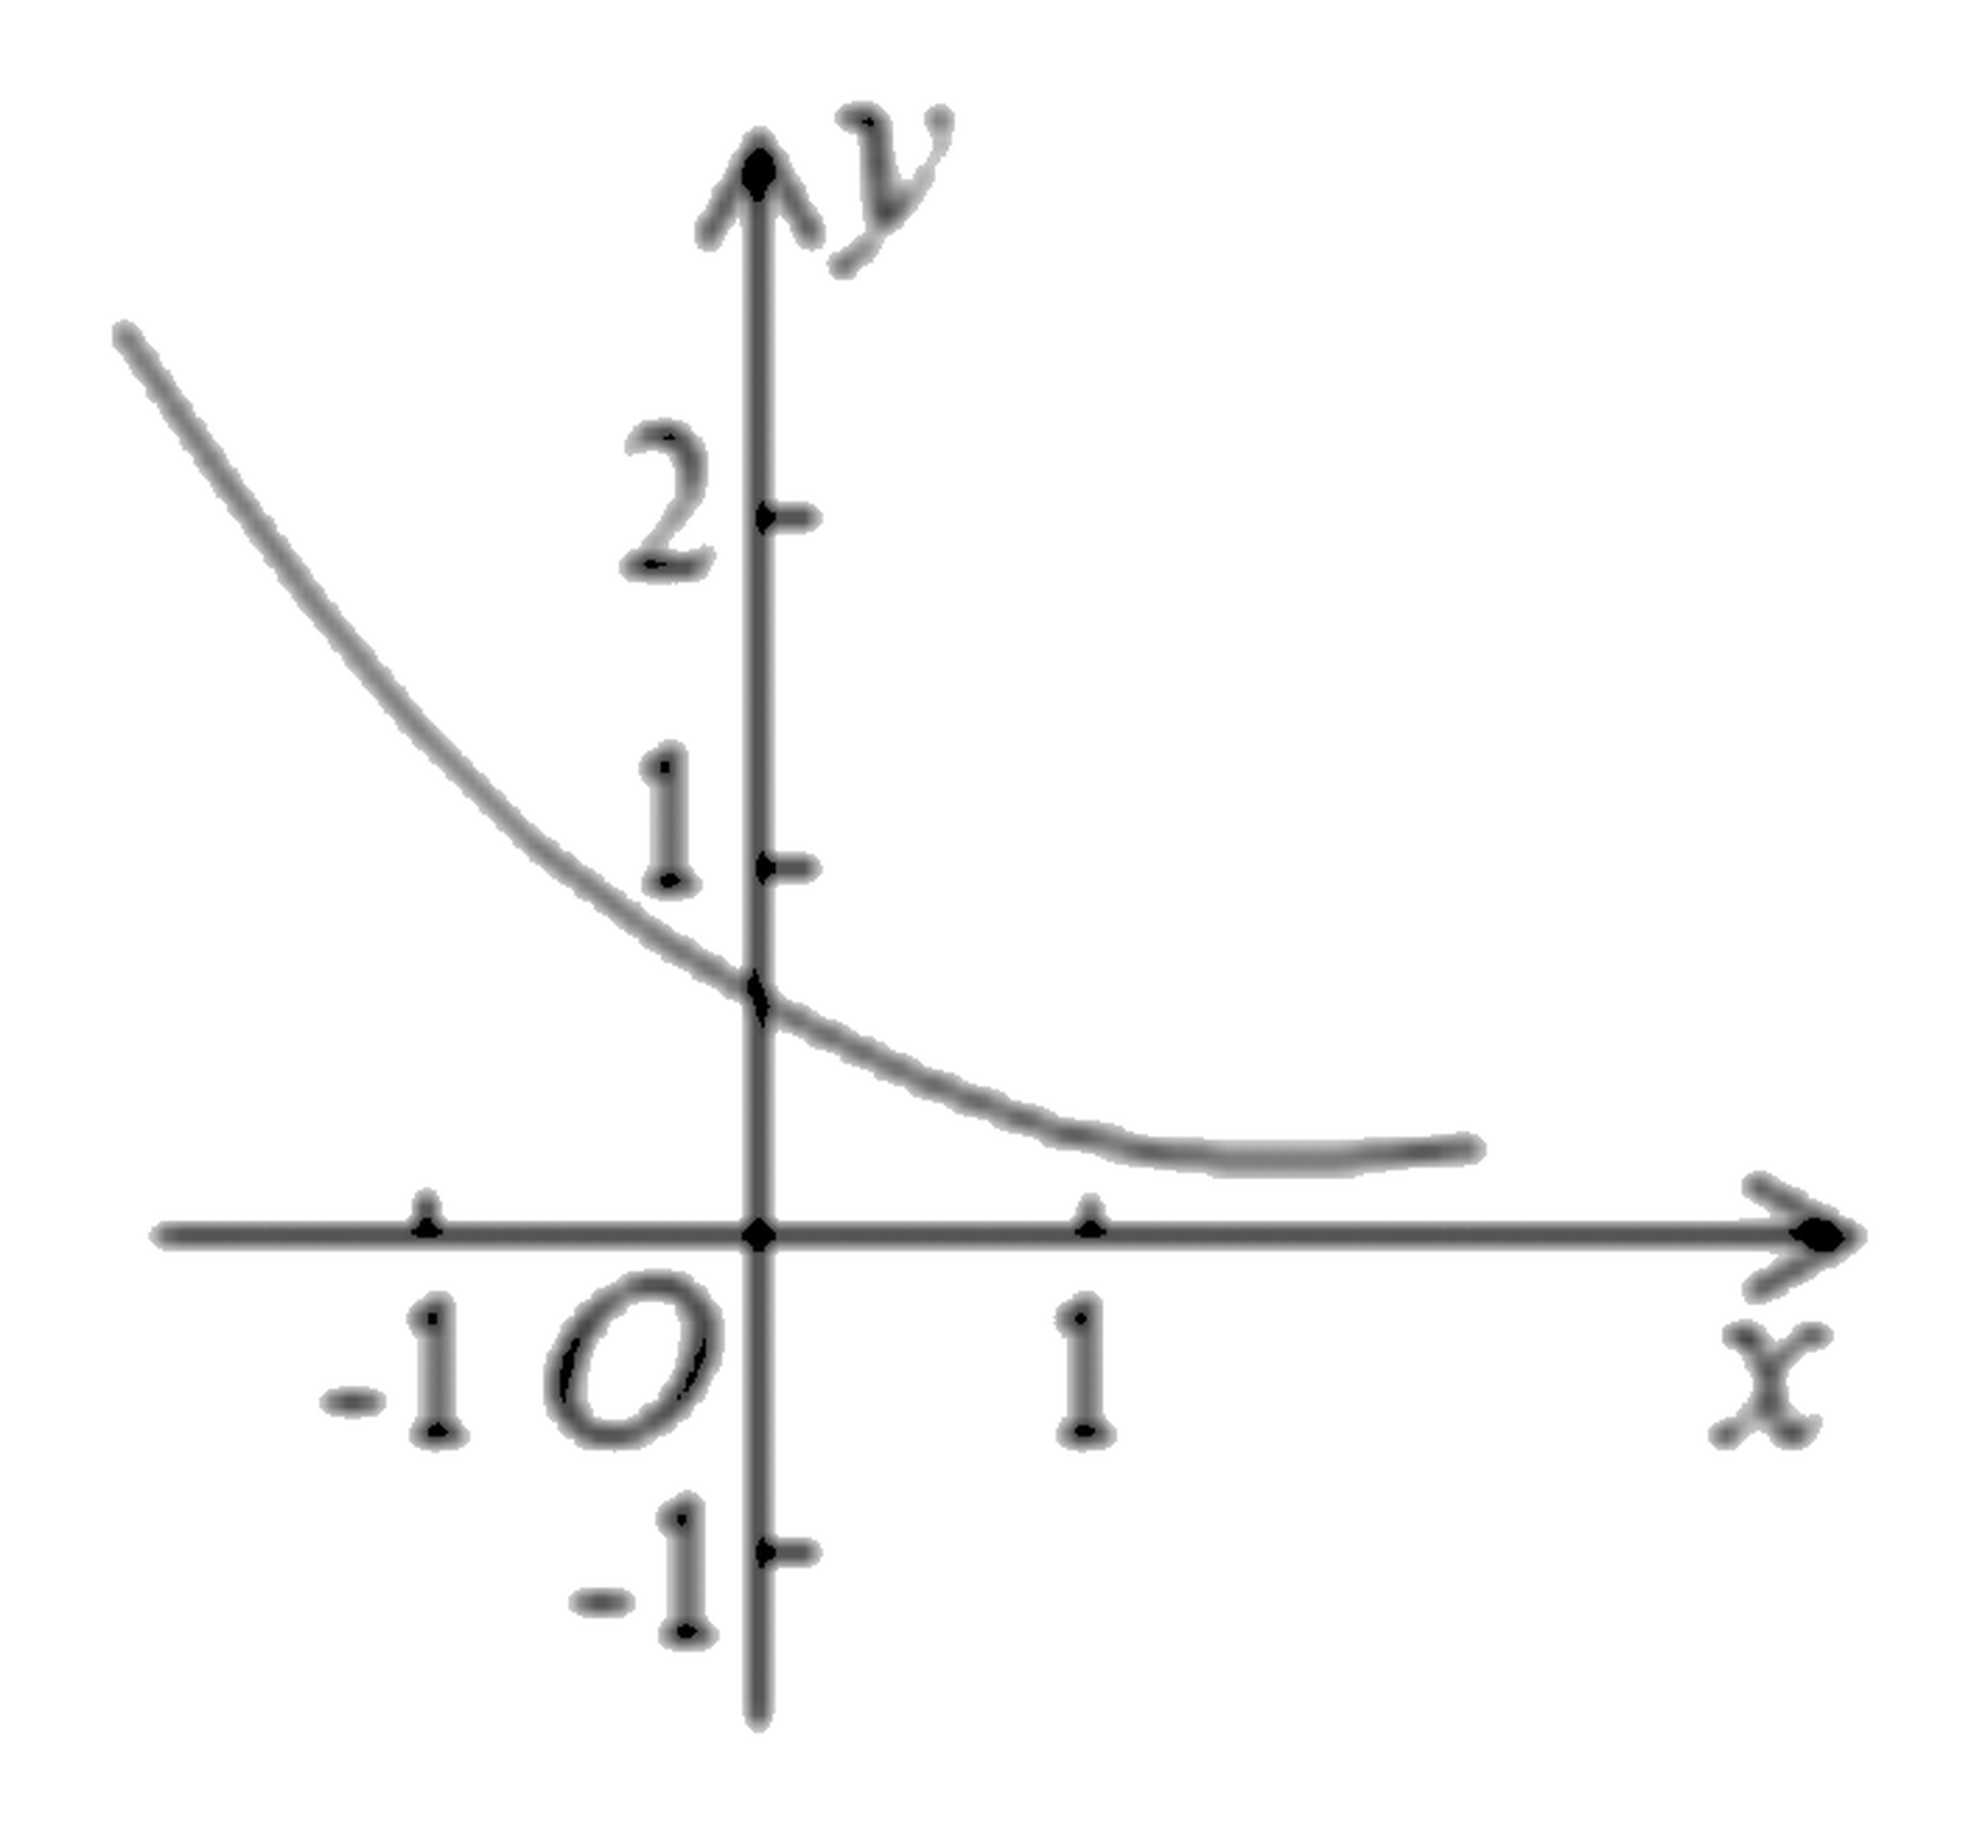
\includegraphics[width=0.30\textwidth]{figures/gao147_q15.png}
\end{center}

\ifanswer
\solbegin
\step{由图象从左到右下降得 $0<a<1$；}
\step{由图象与 $y$ 轴的交点得 $0<a^{-b}<1$，故 $b<0$；}
\step{故 $0<a<1$，$b<0$；故选 $D$.}
\solend
\fi

% === Q16 ===：位数新定义题（无弯引号，放大 04 页 z/q16_stem.png 确认）；四选项横排一行；解析 3 个印刷行
\item 数学运算是指在明晰运算对象的基础上，依据运算法则解决数学问题的素养. 因为运算，数的威力无限；没有运算，数就只是一个符号，对数运算与指数运算是两类重要的运算，对数的运算性质降低了运算的级别，简化了运算，在数学发展史上是伟大的成就. 而位数是指一个自然数有效位的个数，例如：$2^{10}=1024$，所以 $2^{10}$ 的位数为 4. 请你运用所学过的对数运算的知识，估计 $2025^{2026}$ 的位数是\mbox{（\quad）}

\keepwithprev
A. 6697\qquad B. 6698\qquad C. 6699\qquad D. 6700

\ifanswer
\solbegin
\step{设 $2025^{2026}=t$，所以 $\lg t=2026\lg2025$，}
\step{因为 $\lg2025\approx3.3064$，所以 $\lg t\approx6698.8$，}
\step{所以 $t\approx10^{6698.8}\in(10^{6698},10^{6699})$，所以 $2025^{2026}$ 的位数为 6699. 故选 $C$.}
\solend
\fi

\end{enumerate}

\bigsec{三、解答题}

\begin{enumerate}
\setcounter{enumi}{16}

% === Q17 ===：题干＋解析均在 04 页；集合描述竖线 \mid、描述内半角逗号照录；
% 空集 \varnothing、子集 \subseteq（放大 04 页 z/subset_04_q17b.png 确认带下划线）、数集 \R；
% 解析 5 个印刷行，首行末"所以 A=(-∞,-2)∪(3,+∞)"原卷无标点，照录不补
\item 已知集合 $A=\left\{x\mid \dfrac{x+2}{x-3}>0,x\in\R\right\}$，$B=\{x\mid \lvert x-2a\rvert\leqslant2,x\in\R\}$.

(1) 若 $a=1$，求 $A\cap B$；

(2) 若 $A\cap B=\varnothing$，求实数 $a$ 的取值范围.

\ifanswer
\solbegin
\step{由 $\dfrac{x+2}{x-3}>0$，得 $x<-2$ 或 $x>3$，所以 $A=(-\infty,-2)\cup(3,+\infty)$}
\step{(1) 当 $a=1$ 时，$B=\{x\mid \lvert x-2\rvert\leqslant2\}=[0,4]$，于是 $A\cap B=(3,4]$；}
\step{(2) $B=[2a-2,2a+2]$，}
\step{则 $A\cap B=\varnothing\Leftrightarrow[2a-2,2a+2]\subseteq[-2,3]\Leftrightarrow\begin{cases}2a-2\geqslant-2\\2a+2\leqslant3\end{cases}\Leftrightarrow0\leqslant a\leqslant\dfrac{1}{2}$，}
\step{所以实数 $a$ 的取值范围为 $\left[0,\dfrac{1}{2}\right]$.}
\solend
\fi

% === Q18 ===：氟化物／臭氧应用题；"氟化物""（如冰箱等）"全角夹注照录（放大 05 页 z/q18_line1.png 确认）；
% 关系式 $Q=Q_0e^{-0.0025t}$ 原卷独立一行，按一段照录；解析 6 个印刷行
\item 有些家用电器（如冰箱等）使用了氟化物，氟化物的释放破坏了大气上层的臭氧层，使臭氧含量 $Q$ 呈指数函数型变化，在氟化物排放量维持某种水平时，具有关系式

$Q=Q_0e^{-0.0025t}$，其中 $Q_0$ 是臭氧的初始量.

(1) 随时间 $t$ 的增加，臭氧的含量是增加还是减少？

(2) 试估计多少年以后将会有一半的臭氧消失.（用计算器计算）

\ifanswer
\solbegin
\step{(1) 对于函数 $Q=Q_0e^{-0.0025t}$，显然 $Q>0$，}
\step{任取 $t_1$、$t_2\in(0,+\infty)$，且 $t_1<t_2$，则 $t_2-t_1>0$，}
\step{所以 $\dfrac{Q_1}{Q_2}=\dfrac{Q_0e^{-0.0025t_1}}{Q_0e^{-0.0025t_2}}=e^{-0.0025(t_1-t_2)}=e^{0.0025(t_2-t_1)}>e^0=1$，所以 $Q_1>Q_2$，}
\step{故随着时间 $t$ 的增加，臭氧的含量是减少的；}
\step{(2) 令 $\dfrac{Q}{Q_0}=\dfrac{1}{2}$，即 $\dfrac{Q_0e^{-0.0025t}}{Q_0}=e^{-0.0025t}=\dfrac{1}{2}$，得 $-0.0025t=\ln\dfrac{1}{2}\approx-0.6931$，}
\step{解得 $t\approx277$，故估计 277 年以后将会有一半的臭氧消失.}
\solend
\fi

% === Q19 ===：题干用"图像"、解析两处用"图象"逐处照录不统一（05 页）；数集 \Z；
% 题干＋解析前 4 行在 05 页、解析后 3 行在 06 页；解析共 7 个印刷行
\item 已知幂函数 $f(x)=x^{-m^2+4m}(m\in\Z)$ 的图像关于 $y$ 轴对称，且在区间 $(0,+\infty)$ 上是严格增函数.

(1) 求 $m$ 的值；

(2) 求满足不等式 $(2a+1)^m<(a+1)^m$ 的实数 $a$ 的取值范围.

\ifanswer
\solbegin
\step{(1) 由题意得 $-m^2+4m>0$，解得 $0<m<4$，}
\step{因为 $m\in\Z$，所以 $m=1$ 或 $m=2$ 或 $m=3$.}
\step{当 $m=1$ 或 $m=3$ 时，$f(x)=x^3$，图象关于原点对称，不合题意；}
\step{当 $m=2$ 时，$f(x)=x^4$，图象关于 $y$ 轴对称，符合题意，所以 $m=2$.}
\step{(2) 代入 $m=2$，不等式为 $(2a+1)^2<(a+1)^2$，}
\step{得 $(2a+1)^2-(a+1)^2=a(3a+2)<0$，因此 $-\dfrac{2}{3}<a<0$，}
\step{所求范围为 $\left(-\dfrac{2}{3},0\right)$.}
\solend
\fi

% === Q20 ===：指数函数题，题干用"图像"；(3) 长求和式（分数 1/2026、1011/2026、2011/2026、
% 15/2026、1015/2026、2025/2026 放大 06 页 z/q20_sum_06a.png 确认）；题干在 06 页、
% 解析前 6 行在 06 页下半、后 6 行在 07 页上半；解析共 12 个印刷行
\item 已知指数函数 $y=a^x$（$a>0,a\ne1$）的图像经过点 $(1,4)$.

(1) 求实数 $a$ 的值；

(2) 若 $f(x)=(a^x)^2-2\cdot a^x-8$，当 $x\in\R$ 时，不等式 $f(x)>m\cdot4^x-12$ 恒成立，求 $m$ 的取值范围；

(3) 记 $g(x)=\dfrac{1}{a^x+2}$，求证：$g(x)+g(1-x)$ 为定值，并求 $g(0)+g\left(\dfrac{1}{2026}\right)+g\left(\dfrac{1011}{2026}\right)+g\left(\dfrac{2011}{2026}\right)+g\left(\dfrac{1}{2}\right)+g\left(\dfrac{15}{2026}\right)+g\left(\dfrac{1015}{2026}\right)+g\left(\dfrac{2025}{2026}\right)+g(1)$ 的值.

\ifanswer
\solbegin
\step{(1) 将 $(1,4)$ 代入 $y=a^x$，得 $a^1=4$，即 $a=4$.}
\step{(2) 令 $t=4^x$，当 $x\in\R$ 时，$t$ 取遍所有正实数.}
\step{原不等式等价于 $t^2-2t-8>mt-12\Leftrightarrow m<t+\dfrac{4}{t}-2$，}
\step{由基本不等式，$t+\dfrac{4}{t}-2\geqslant2\sqrt{t\cdot\dfrac{4}{t}}-2=2$，}
\step{当且仅当 $t=\dfrac{4}{t}$，即 $t=2$ 时取等号，}
\step{因此原不等式恒成立的充要条件为 $m<2$，即 $m\in(-\infty,2)$.}
\step{(3) 对任意 $x\in\R$，令 $t=4^x>0$，则 $4^{1-x}=\dfrac{4}{t}$，}
\step{从而 $g(x)+g(1-x)=\dfrac{1}{t+2}+\dfrac{1}{\dfrac{4}{t}+2}=\dfrac{1}{t+2}+\dfrac{t}{2(t+2)}=\dfrac{1}{2}$，}
\step{因此 $g(x)+g(1-x)$ 为定值 $\dfrac{1}{2}$.}
\step{原式中，0 与 1、$\dfrac{1}{2026}$ 与 $\dfrac{2025}{2026}$、$\dfrac{1011}{2026}$ 与 $\dfrac{1015}{2026}$、$\dfrac{2011}{2026}$ 与 $\dfrac{15}{2026}$}
\step{分别配对，每对函数值之和均为 $\dfrac{1}{2}$，且 $g\left(\dfrac{1}{2}\right)=\dfrac{1}{4^{\frac12}+2}=\dfrac{1}{4}$，}
\step{所以所求和为 $4\cdot\dfrac{1}{2}+\dfrac{1}{4}=\dfrac{9}{4}$.}
\solend
\fi

% === Q21 ===：不动点新定义题；题干在 07 页、解析续 08／09 页，共 20 个印刷行；
% 判别式两形混用：08 页 (2) cases 内等腰偏高 \Delta、09 页 (3) 扁等边 \triangle，逐处照录不统一
% （放大 /tmp/gao147/z/delta_vs_triangle.png 并排确认）；数集 \R；\forall 照录；
% 第 6—8 行是原卷一个长算式折成的三个印刷行，按印刷行分三条 \step、不并折行
\item 对于二次函数 $y=mx^2+nx+t(m\ne0)$，若存在 $x_0\in\R$，使得 $mx_0^2+nx_0+t=x_0$ 成立，则称 $x_0$ 为二次函数 $y=mx^2+nx+t(m\ne0)$ 的不动点.

(1) 求二次函数 $y=x^2-x-3$ 的不动点；

(2) 若二次函数 $y=2x^2-(3+a)x+a-1$ 有两个不相等的不动点 $x_1$、$x_2$，且 $x_1$、$x_2>0$，求 $\dfrac{x_1}{x_2}+\dfrac{x_2}{x_1}$ 的最小值；

(3) 若对任意实数 $b$，二次函数 $y=ax^2+(b+1)x+(b-1)(a\ne0)$ 恒有不动点，求 $a$ 的取值范围.

\ifanswer
\solbegin
\step{(1) 令 $x^2-x-3=x$，即 $x^2-2x-3=0$，即 $(x-3)(x+1)=0$，}
\step{解得 $x_1=-1$，$x_2=3$，所以不动点为 $-1$ 和 $3$.}
\step{(2) 由题意，$2x^2-(3+a)x+a-1=x$ 有两个不相等的正实数根，}
\step{即方程 $2x^2-(4+a)x+a-1=0$ 有两个不相等的正实数根，}
\step{所以 $\begin{cases}\Delta=(4+a)^2-8(a-1)>0\\x_1+x_2=\dfrac{4+a}{2}>0\\x_1\cdot x_2=\dfrac{a-1}{2}>0\end{cases}$，解得 $a>1$，}% 判别式原卷印等腰偏高粗三角 $\Delta$（放大 08 页 z/delta_08_q21cases.png）
\step{所以 $\dfrac{x_1}{x_2}+\dfrac{x_2}{x_1}=\dfrac{x_1^2+x_2^2}{x_1\cdot x_2}=\dfrac{(x_1+x_2)^2-2x_1\cdot x_2}{x_1\cdot x_2}=\dfrac{(x_1+x_2)^2}{x_1\cdot x_2}-2$}
\step{$=\dfrac{\left(\dfrac{4+a}{2}\right)^2}{\dfrac{a-1}{2}}-2=\dfrac{\dfrac{(a+4)^2}{4}}{\dfrac{a-1}{2}}-2=\dfrac{(a-1+5)^2}{2(a-1)}-2$}
\step{$=\dfrac{(a-1)^2+10(a-1)+25}{2(a-1)}-2=\dfrac{a-1}{2}+\dfrac{25}{2(a-1)}+3$.}
\step{因为 $a>1$，所以 $a-1>0$，}
\step{所以 $\dfrac{a-1}{2}+\dfrac{25}{2(a-1)}+3\geqslant2\sqrt{\dfrac{a-1}{2}\cdot\dfrac{25}{2(a-1)}}+3=8$，}
\step{当且仅当 $\dfrac{a-1}{2}=\dfrac{25}{2(a-1)}$，即 $a=6$ 时等号成立，}
\step{所以 $\dfrac{x_1}{x_2}+\dfrac{x_2}{x_1}$ 的最小值为 $8$.}
\step{(3) 设 $f(x)=ax^2+(b+1)x+b-1$，}
\step{则方程 $f(x)=x$，可化为 $ax^2+(b+1)x+b-1=x$，}
\step{即 $ax^2+bx+b-1=0$，}
\step{由题意得一元二次方程 $ax^2+bx+b-1=0$ 有解，又 $a\ne0$，}
\step{所以方程 $ax^2+bx+b-1=0$ 的判别式 $\triangle=b^2-4a(b-1)\geqslant0$，}% 判别式原卷印扁等边细线三角 $\triangle$（放大 09 页 z/triangle_09_q21.png），与 (2) 高 $\Delta$ 混用、照录不统一
\step{即 $b^2-4ab+4a\geqslant0$，则该不等式对 $\forall b\in\R$ 恒成立，}
\step{则 $(4a)^2-4\times4a\leqslant0$，且 $a\ne0$，解得 $0<a\leqslant1$，}
\step{所以实数 $a$ 的取值范围是 $(0,1]$.}
\solend
\fi

\end{enumerate}

\end{document}
"
% 紧凑版：xelatex "\def\iscompact{1}% 高一147_华师大三附中_期中.tex
%   —— 高一上数学"2026-2027 年华师大三附中高一上期中"（试卷版/答案版/紧凑版）
% 试卷版：xelatex 高一147_华师大三附中_期中.tex
% 答案版：xelatex "\def\isanswer{1}\input{高一147_华师大三附中_期中.tex}"
% 紧凑版：xelatex "\def\iscompact{1}\input{高一147_华师大三附中_期中.tex}"
%
% ① 原始材料：微信公众号"魔都数学加油站"文章，连载"27学年高一147"，原文标题
% "27学年高一147——2026-2027年上海市华师大三附中高一上期中"；
% 原文链接：https://mp.weixin.qq.com/s/X_gPW1JWoTAl2Bky_xEEGw 。
% 正文为 9 张 PNG 页（01/06/08/09 为 2560×3620，02/03/04/05/07 为 4762×6735，
% 同一篇各页分辨率混排，逐页按各自分辨率裁图核对，别按预览比例换算裁框）。
% 体例：混合体例讲评版——19 题中 Q4/Q5/Q7/Q9 只印【答案】、无【解析】，其余 15 题印
% 【解析】（逐题核实，见 ② ②）。题目、答案、解析均据原图转录；卷面粉红色水印
% "魔都数学加油站"及公众号页脚未录入。
% 全卷插图清单（逐页通读 9 页确认）：仅 1 处题目配图——
%   · Q15 递减指数函数小坐标系（03 页右侧：坐标轴、y 轴刻度 2/1/-1、x 轴刻度 -1/1、
%     原点 O、x/y 轴标），为"图像如图所示"的题目配图（选择题选项旁），三版都出；
%     裁自 03 页去粉色水印、去色、4× LANCZOS 放大存 figures/gao147_q15.png；
%   其余 8 页逐页确认无其它题目配图、无【解析】内配图、无表格，
%   亦无"题干写如图而源码漏图"一处；Q12/Q17/Q21 的 cases 块为数学块（非图）。
%
% 卷首标题：原卷印作"2026-2027 年华师大三附中高一上期中"，年份区间按全稿惯例排 en dash；
% 原卷卷面未印副标题，本稿按同期中卷（高一140／141／143／144／145／146）知识模块口径
% 补出"集合与常用逻辑用语、不等式、函数"。
%
% 题号体例（逐页核实定稿）：本卷共 19 题——一、填空题 3—12（10 题）、
% 二、选择题 13—16（4 题）、三、解答题 17—21（5 题）。
% 三节分别 \setcounter{enumi}{2}／{12}／{16}。原卷从第 3 题起、无第 1、2 题，
% 本稿保留原题号；全卷无附加题节（Q21 解析末行"所以实数 a 的取值范围是 (0,1]."
% 为全卷收尾，09 页下半仅水印、无正文）。
%
% ② 与原卷的排版差异：
%   ① 原文从第 3 题起，本稿保留原题号；共 19 题三节；
%   ② 混合体例：原卷 Q4/Q5/Q7/Q9 只印【答案】、无【解析】（分别为 a≤0、(-1,2)、
%      真、(-∞,1)），按 高一140 第 5 题／高一145 Q3 成例提 \ans{}、不补造解析；
%      其余 15 题印【解析】，用 \solbegin…\solend，选择题答案在解析末句"故选 X"
%      （Q13 选 B、Q14 选 B、Q15 选 D、Q16 选 C，逐个放大原图核实）、题干括号
%      \mbox{（\quad）} 留空、不另提 \ans{}；填空／解答答案落在解析里；
%      答案版【答案】/【解析】标记数 = 19（4 个 \ans ＋ 15 个 \solbegin）= 全卷题数；
%   ③ 原卷卷面未印副标题，本稿按知识模块口径补出；
%   ④ 原卷填空横线按全稿惯例排 \blankline[4.4em]；选择题括号排 \mbox{（\quad）}、
%      选项段前按惯例加 \keepwithprev；Q14／Q15 四选项为 2×2 两印刷行（A/B 一行、
%      C/D 一行），用空行分段照录（非一行 \qquad、亦非竖排四行）；解答题不留作答区、
%      不加 \anspace（原卷为讲评版，与 129／131／132／133／136／140／141／143／144／145／146 同）；
%   ⑤ 数集：Q4"A∪B=R"、Q13"f(x)=x^3 在 R 上严格增"、Q17"x∈R"两处、
%      Q20"x∈R"两处、Q21"x_0∈R""∀b∈R"原卷印斜体或黑板粗体 R，按全稿惯例统一改 \R；
%      Q19"m∈Z"改 \Z；本卷未出现 N（\N^* 无对应处）。绝对值排 \lvert…\rvert，
%      集合描述竖线排 \mid；不等号按全稿惯例排 \leqslant／\geqslant（原卷印 \le／\ge 形，
%      【答案】a≤0 亦排 \leqslant）；空集 \varnothing（Q17 两处）；
%      子集 \subseteq（Q17 带下划线，放大 04 页确认）；本卷未出现 \subset／\subsetneq，
%      亦未出现补集上划线 \overline{}；\left…\right 不得拆到不同 $…$ 组；
%   ⑥ 子题标号 (1)(2)(3) 半角括号照录；cases 块整体算一个印刷行（Q3、Q12 一行内
%      两个 cases、Q17、Q21(2)）；本卷解析内无圈数字①②③（无 \text{①} 需求）；
%      数学式内 CJK 用 \text{}（本卷未见）；
%   ⑦ 题干中的中文弯引号按原卷照录：Q7 命题"若 A∪B=B，则 A∩B=A"与
%      (填 " 真 " 或 " 假 ")、Q10 (填 ">" "<" "≤" "或≥")，含引号内空格；
%      注释内一律 ASCII 引号；Q16 位数新定义题逐字放大确认无弯引号
%      （交办提示的"Q16 新定义题"举例未在本卷出现），未补造引号；
%   ⑧ 半角逗号在数学组之间是全稿惯例、非笔误（Q4"$A=(-\infty,0],B=[a,+\infty)$"、
%      Q5"$(a>0,a\ne1)$"、Q17 集合描述内"$>0,x\in R$""$\leqslant2,x\in R$"、
%      Q20 题干"$(a>0,a\ne1)$"、Q21"$y=mx^2+nx+t(m\ne0)$"等），逐处照录别改全角；
%      行末西文句点照录为 ASCII `.`；行中全角逗号／顿号照录；
%      Q7／Q10"(填…)"为半角括号、Q18"（如冰箱等）"为全角括号，逐处照录不统一；
%   ⑨ "图像／图象"逐处照录不统一：题干 5 处用"图像"（Q5"图像恒过定点"、
%      Q9"图像位于直线 y=x 的下方"、Q15"的图像如图所示"、Q19"的图像关于 y 轴对称"、
%      Q20"的图像经过点"），解析 4 处用"图象"（Q15"由图象从左到右下降"
%      "由图象与 y 轴的交点"、Q19"图象关于原点对称""图象关于 y 轴对称"），逐处核、不统一；
%   ⑩ 判别式 Δ/△ 混用是照录项：Q21(2) 解析 cases 块"Δ=(4+a)²−8(a−1)>0"
%      印等腰偏高粗三角 \Delta，Q21(3) 解析"判别式△=b²−4a(b−1)≥0"
%      印扁等边细线三角 \triangle，逐处放大判断、照录不得统一
%      （参照 高一142／144／145 头注④口径，详见 ④）；
%   ⑪ 一条 \step = 原卷解析的一个印刷行，cases 块整体算一个印刷行；别把原卷折行
%      并起来、别把一行拆多条。Q10 七行（跨 01→02 页）、Q12 七行（含一行两 cases）、
%      Q20 十二行（含"原式中…2011/2026 与 15/2026／分别配对…"折行两行）、
%      Q21 二十行（含第 6—8 行一个长算式折成三印刷行、含 cases）均按印刷行逐条断，
%      不丢行；
%   ⑫ 配图：逐页通读 9 页确认全卷仅 Q15 一处题目配图（见 ①），三版都出、
%      \includegraphics[width=0.30\textwidth]；图块较小，未加 \needvspace 大图块守卫
%      （仅 \bigsec 自带 \needvspace{3\baselineskip}）；三版切页审计均"合计异常：无"；
%   ⑬ 跨页续印按题合并：Q3—Q9 在 01 页（Q10 题干在 01 页末、解析首行亦在 01 页末）；
%      Q10 解析续 02 页 6 行、Q11 在 02 页、Q12 题干＋解析前 4 行在 02 页
%      （解析续 03 页 3 行）；"二、选择题"标题与 Q13、Q14、Q15 题干＋解析前 2 行在 03 页
%      （Q15 配图在 03 页右侧）；Q15 解析末行与 Q16、"三、解答题"标题、Q17 在 04 页；
%      Q18 在 05 页、Q19 题干＋解析前 4 行在 05 页（解析续 06 页 3 行）；
%      Q20 题干＋解析前 6 行在 06 页（解析续 07 页 6 行）、Q21 题干＋解析前 3 行在 07 页；
%      Q21 解析续 08 页 13 行、续 09 页 4 行（09 页下半仅水印、无正文）。
%      本稿按题连排，不丢行、不并折行；
%   ⑭ 原卷解析内无红色"法一／法二"之类小标题，故本卷无 \stepm；
%      水印"魔都数学加油站"红色不录入。
%
% ③ 行数复核：一条 \step／\stepm = 原卷解析的一个印刷行，cases 块作一个印刷行计。
%   逐题数（主会话逐页核对定稿）：Q3：1；Q4：0（只印【答案】、提 \ans{}，不计入 \step 账）；
%   Q5：0；Q6：1；Q7：0；Q8：2；Q9：0；Q10：7；Q11：4；Q12：7；Q13：6；Q14：4；
%   Q15：3；Q16：3；Q17：5；Q18：6；Q19：7；Q20：12；Q21：20。
%   合计 88 条 \step（本卷无 \stepm：解析内无红色"法一／法二"类小标题），
%   与原卷逐题印刷行相等。全卷 15 题设 \solbegin…\solend ＋ 4 题一处 \ans{}，
%   答案版【答案】/【解析】标记数 = 19 = 全卷题数。
%
% ④ 判别式／子集符号结论（逐处放大原图照录、不得统一，主会话像素级复核）：
%   判别式全卷 2 处、两形混用逐处照录不统一（参照 高一142／144 头注④口径）：
%     · Q21(2) 解析 cases 块"Δ=(4+a)²−8(a−1)>0" 原卷印等腰偏高粗三角
%       （高>宽、粗笔画），照录 \Delta（放大 08 页 /tmp/gao147/z/delta_08_q21cases.png
%       与 z/delta_vs_triangle.png 左图确认）；
%     · Q21(3) 解析"判别式△=b²−4a(b−1)≥0" 原卷印扁等边细线三角
%       （宽≈高、细线），照录 \triangle（放大 09 页 /tmp/gao147/z/triangle_09_q21.png
%       与 z/delta_vs_triangle.png 右图并排确认）。
%   子集／补集：Q17 解析"[2a−2,2a+2]⊆[−2,3]" 原卷印带下划线 ⊆，照录 \subseteq
%     （放大 04 页 /tmp/gao147/z/subset_04_q17b.png 确认）；Q17"A∩B=∅"空集 \varnothing；
%     集合描述竖线 \mid（Q10 M、Q12 解集、Q17 A/B）；并集 \cup（Q4、Q17）、
%     交集 \cap（Q7、Q17）、不属于 \notin（Q10）；数集 \R／\Z 归一见 ② ⑤。
%   本卷未出现 \subset／\subsetneq，未出现补集上划线 \overline{}。
%
% ⑤ 存疑照录（放大原图确认，照录未改、正文对应处另有 % 注）：
%   1. Q4/Q5/Q7/Q9 只印【答案】、无【解析】，按成例提 \ans{}、不补造解析
%      （混合体例逐题核实，见 ② ②）。
%   2. Q21(2) 判别式高 \Delta 与 Q21(3) 判别式扁 \triangle 两形混用，
%      逐处照录不统一（见 ④）。
%   3. "图像／图象"题干 5 处"图像"、解析 4 处"图象"，逐处照录不统一（见 ② ⑨）。
%   4. Q7／Q10"(填…)"半角括号与 Q18"（如冰箱等）"全角括号，逐处照录不统一。
%   5. Q16 位数新定义题逐字放大确认无弯引号（交办提示的"Q16 新定义题"举例
%      未在本卷出现），未补造引号；全卷弯引号仅 Q7、Q10 两处。
%   6. Q17 解析首行末"所以 A=(-∞,-2)∪(3,+∞)"、Q20(3) 解析"…2011/2026 与 15/2026"
%      行末原卷均无标点，照录未补；Q21(2) 第 6—8 行一个长算式折成三印刷行，
%      按印刷行分三条 \step、不并折行。
%   全卷除此 6 类外未发现其它笔误／自相矛盾处。
%
% ⑥ 跨页续印按题合并说明：见 ② ⑬。
%
\documentclass[a4paper,11pt]{article}
\usepackage{common}

\begin{document}

\examtitlest[3]{2026--2027 年华师大三附中高一上期中}{集合与常用逻辑用语、不等式、函数}

\bigsec{一、填空题}

\begin{enumerate}
\setcounter{enumi}{2}

% === Q3 ===：印【解析】，1 个印刷行（cases 块整体算一行）
\item 函数 $y=(a^2-5a+7)a^x+6-2a$ 是指数函数，则 $a$ 的值为\blankline[4.4em].

\ifanswer
\solbegin
\step{由题意得 $\begin{cases}a^2-5a+7=1\\6-2a=0\end{cases}$，解得 $a=3$.}
\solend
\fi

% === Q4 ===：原卷只印【答案】、无【解析】，按 高一140 第 5 题／高一145 Q3 成例提 \ans{}、不补造解析；
% 题干数学组内半角逗号 $A=(-\infty,0],B=[a,+\infty)$ 照录（放大 01 页 z/q4_stem.png 确认）
\item 已知 $A=(-\infty,0],B=[a,+\infty)$，且 $A\cup B=\R$，则实数 $a$ 的取值范围为\blankline[4.4em].

\ifanswer
\ans{$a\leqslant0$}
\fi

% === Q5 ===：只印【答案】；题干"图像"照录（放大 01 页 z/q5_stem.png 确认）；
% 数学组内半角逗号 $(a>0,a\ne1)$ 照录
\item 函数 $y=a^{x+1}+1(a>0,a\ne1)$ 的图像恒过定点\blankline[4.4em].

\ifanswer
\ans{$(-1,2)$}
\fi

% === Q6 ===：印【解析】，1 个印刷行
\item 已知方程 $x^2+2x-4=0$ 的两个根为 $x_1$、$x_2$，则 $x_1^2+x_2^2$ 的值为\blankline[4.4em].

\ifanswer
\solbegin
\step{$x_1^2+x_2^2=(x_1+x_2)^2-2x_1x_2=4+8=12$.}
\solend
\fi

% === Q7 ===：只印【答案】；中文弯引号"若 A∪B=B，则 A∩B=A"与(填 " 真 " 或 " 假 ")内的空格照录
% （放大 01 页 z/q7_quotes_7x.png、z/q7_tail.png 确认，括号为半角）
\item 命题 “若 $A\cup B=B$，则 $A\cap B=A$” 为\blankline[4.4em]命题(填 “ 真 ” 或 “ 假 ”).

\ifanswer
\ans{真}
\fi

% === Q8 ===：印【解析】，2 个印刷行；不等号按全稿惯例 \geqslant／\leqslant
\item 已知正实数 $a$、$b$ 满足 $a+4b=1$，则 $ab$ 的最大值为\blankline[4.4em].

\ifanswer
\solbegin
\step{$a+4b\geqslant2\sqrt{a\cdot4b}\Rightarrow ab\leqslant\dfrac{1}{16}$，当且仅当 $a=4b=\dfrac{1}{2}$ 时取等号，}
\step{则 $ab$ 的最大值为 $\dfrac{1}{16}$.}
\solend
\fi

% === Q9 ===：只印【答案】；题干"图像"照录（放大 01 页 hi_01_2 确认）
\item 若幂函数 $y=x^s$ 在 $x>1$ 时的图像位于直线 $y=x$ 的下方，则 $s$ 的取值范围是\blankline[4.4em].

\ifanswer
\ans{$(-\infty,1)$}
\fi

% === Q10 ===：印【解析】，共 7 个印刷行（题在 01 页末起 1 行、续 02 页 6 行）；
% 题干跨两印刷行"则 |ab|+1 ____ |a|+|b|（填…）"按一句连排；(填…)为半角括号、引号内空格照录
\item 已知不等式 $\lvert2x+1\rvert+\lvert2x-1\rvert<4$ 的解集为 $M$. 设实数 $a\in M$，$b\notin M$，则 $\lvert ab\rvert+1$\blankline[4.4em] $\lvert a\rvert+\lvert b\rvert$(填 “$>$”，“$<$”，“$\leqslant$” “或$\geqslant$”).

\ifanswer
\solbegin
\step{当 $x<-\dfrac{1}{2}$ 时，不等式化为 $-2x-1+1-2x<4$，即 $x>-1$，所以 $-1<x<-\dfrac{1}{2}$；}
\step{当 $-\dfrac{1}{2}\leqslant x\leqslant\dfrac{1}{2}$ 时，不等式化为 $2x+1-2x+1<4$，即 $2<4$，所以 $-\dfrac{1}{2}\leqslant x\leqslant\dfrac{1}{2}$；}
\step{当 $x>\dfrac{1}{2}$ 时，不等式化为 $2x+1+2x-1<4$，即 $x<1$，所以 $\dfrac{1}{2}<x<1$；}
\step{综上，$M=\{x\mid -1<x<1\}$.}
\step{因为 $a\in M$，$b\notin M$，所以 $\lvert a\rvert<1$，$\lvert b\rvert\geqslant1$.}
\step{而 $\lvert ab\rvert+1-(\lvert a\rvert+\lvert b\rvert)=\lvert ab\rvert+1-\lvert a\rvert-\lvert b\rvert=(\lvert a\rvert-1)(\lvert b\rvert-1)$，}
\step{所以 $\lvert ab\rvert+1\leqslant\lvert a\rvert+\lvert b\rvert$.}
\solend
\fi

% === Q11 ===：印【解析】，4 个印刷行（02 页）
\item 已知 $m>1$，$n>1$，$\lg m=\log_n100$，则 $mn$ 的最小值为\blankline[4.4em].

\ifanswer
\solbegin
\step{由 $m>1$，$n>1$，得 $\lg m>0$，$\lg n>0$，}
\step{因为 $\lg m=\log_n100=\dfrac{\lg100}{\lg n}=\dfrac{2}{\lg n}$，所以 $\lg m\cdot\lg n=2$，}
\step{所以 $\lg(mn)=\lg m+\lg n\geqslant2\sqrt{\lg m\cdot\lg n}=2\sqrt2$，}
\step{当且仅当 $m=n=10^{\sqrt2}$ 时取等号，则 $mn\geqslant10^{2\sqrt2}$，即 $mn$ 的最小值为 $10^{2\sqrt2}$.}
\solend
\fi

% === Q12 ===：印【解析】，共 7 个印刷行（02 页 4 行、03 页 3 行）；
% 第 3 行"则 [cases]，得 [cases]，"两个 cases 块同属一个印刷行，整体作一条 \step（照 高一146 Q11 成例）
\item 已知关于 $x$ 的不等式 $ax^2+bx+c\leqslant1$ 的解集为 $\{x\mid -1\leqslant x\leqslant3\}$. 若关于 $x$ 的不等式 $ax^2+(b-1)x+c-2\leqslant0$ 有且仅有 8 个整数解，则实数 $a$ 的取值范围是\blankline[4.4em].

\ifanswer
\solbegin
\step{由已知关于 $x$ 的不等式 $ax^2+bx+c\leqslant1$ 的解集为 $\{x\mid -1\leqslant x\leqslant3\}$，}
\step{得 $a>0$，且方程 $ax^2+bx+c-1=0$ 的两根分别为 $-1$ 和 $3$，}
\step{则 $\begin{cases}-1+3=-\dfrac{b}{a}\\-1\times3=\dfrac{c-1}{a}\end{cases}$，得 $\begin{cases}b=-2a\\c=1-3a\end{cases}$，}
\step{不等式 $ax^2+(b-1)x+c-2\leqslant0$ 等价于 $ax^2-(2a+1)x-(3a+1)\leqslant0$，}
\step{即 $\left[x-\left(3+\dfrac{1}{a}\right)\right](x+1)\leqslant0$，解得 $-1\leqslant x\leqslant3+\dfrac{1}{a}$，}
\step{因为关于 $x$ 的不等式 $ax^2+(b-1)x+c-2\leqslant0$ 有且仅有 8 个整数解，}
\step{因此 $6\leqslant3+\dfrac{1}{a}<7$，即 $3\leqslant\dfrac{1}{a}<4$，解得 $\dfrac{1}{4}<a\leqslant\dfrac{1}{3}$，所以 $a$ 的取值范围为 $\left(\dfrac{1}{4},\dfrac{1}{3}\right]$.}
\solend
\fi

\end{enumerate}

\bigsec{二、选择题}

\begin{enumerate}
\setcounter{enumi}{12}

% === Q13 ===：题干＋选项＋解析均在 03 页；四选项横排一行；解析 6 个印刷行，末句"故选 B."
\item $a<b<0$，则下列不等式能成立的是\mbox{（\quad）}

\keepwithprev
A. $\dfrac{a}{b}<1$\qquad B. $\lvert a\rvert>-b$\qquad C. $\dfrac{1}{a}<\dfrac{1}{b}$\qquad D. $b^3<a^3$

\ifanswer
\solbegin
\step{对于 $A$，令 $a=-4$，$b=-3$，满足 $a<b<0$，但 $\dfrac{a}{b}>1$，故 $A$ 错误，}
\step{对于 $B$，因为 $a<b<0$，所以 $-a>-b>0$，即 $\lvert a\rvert>-b$，故 $B$ 正确，}
\step{对于 $C$，令 $a=-4$，$b=-3$，满足 $a<b<0$，但 $\dfrac{1}{a}>\dfrac{1}{b}$，故 $C$ 错误，}
\step{对于 $D$，$f(x)=x^3$ 在 $\R$ 上严格增，因为 $a<b$，所以 $f(a)<f(b)$，}
\step{即 $a^3<b^3$，故 $D$ 错误.}
\step{故选 $B$.}
\solend
\fi

% === Q14 ===：四选项原卷为 2×2 两印刷行（A/B 一行、C/D 一行），用空行分段照录；解析 4 个印刷行
\item 已知 $a$、$b$ 为实数，若 $\alpha:ab=0$，$\beta:a^2+\sqrt{b}=0$，则 $\alpha$ 是 $\beta$ 的\mbox{（\quad）}

\keepwithprev
A. 充分不必要条件\qquad\qquad B. 必要不充分条件

C. 充要条件\qquad\qquad D. 既不充分也不必要条件

\ifanswer
\solbegin
\step{$\beta:a^2+\sqrt{b}=0$，所以 $a=0$ 且 $b=0$，}
\step{由 $a=0$，$b=0\Rightarrow ab=0$，反之不成立.}
\step{所以 $ab=0$ 是 $a=0$，$b=0$ 的必要不充分条件，即 $\alpha$ 是 $\beta$ 的必要不充分条件，}
\step{故选 $B$.}
\solend
\fi

% === Q15 ===：题目配图（03 页右侧小坐标系），三版都出；题干用"图像"、解析用"图象"逐处照录；
% 四选项 2×2 两印刷行；解析 3 个印刷行（03 页 2 行、04 页 1 行，末句"故选 D."与前行同一印刷行）
\item 函数 $f(x)=a^{x-b}$ 的图像如图所示，其中 $a$、$b$ 为常数，则下列结论正确的是\mbox{（\quad）}

\keepwithprev
A. $a>1$，$b<0$\qquad\qquad B. $a>1$，$b>0$

C. $0<a<1$，$b>0$\qquad\qquad D. $0<a<1$，$b<0$

\begin{center}
% 递减指数函数小坐标系图取 03 页右侧，去粉色水印、去色、4× LANCZOS 放大；题目配图三版都出
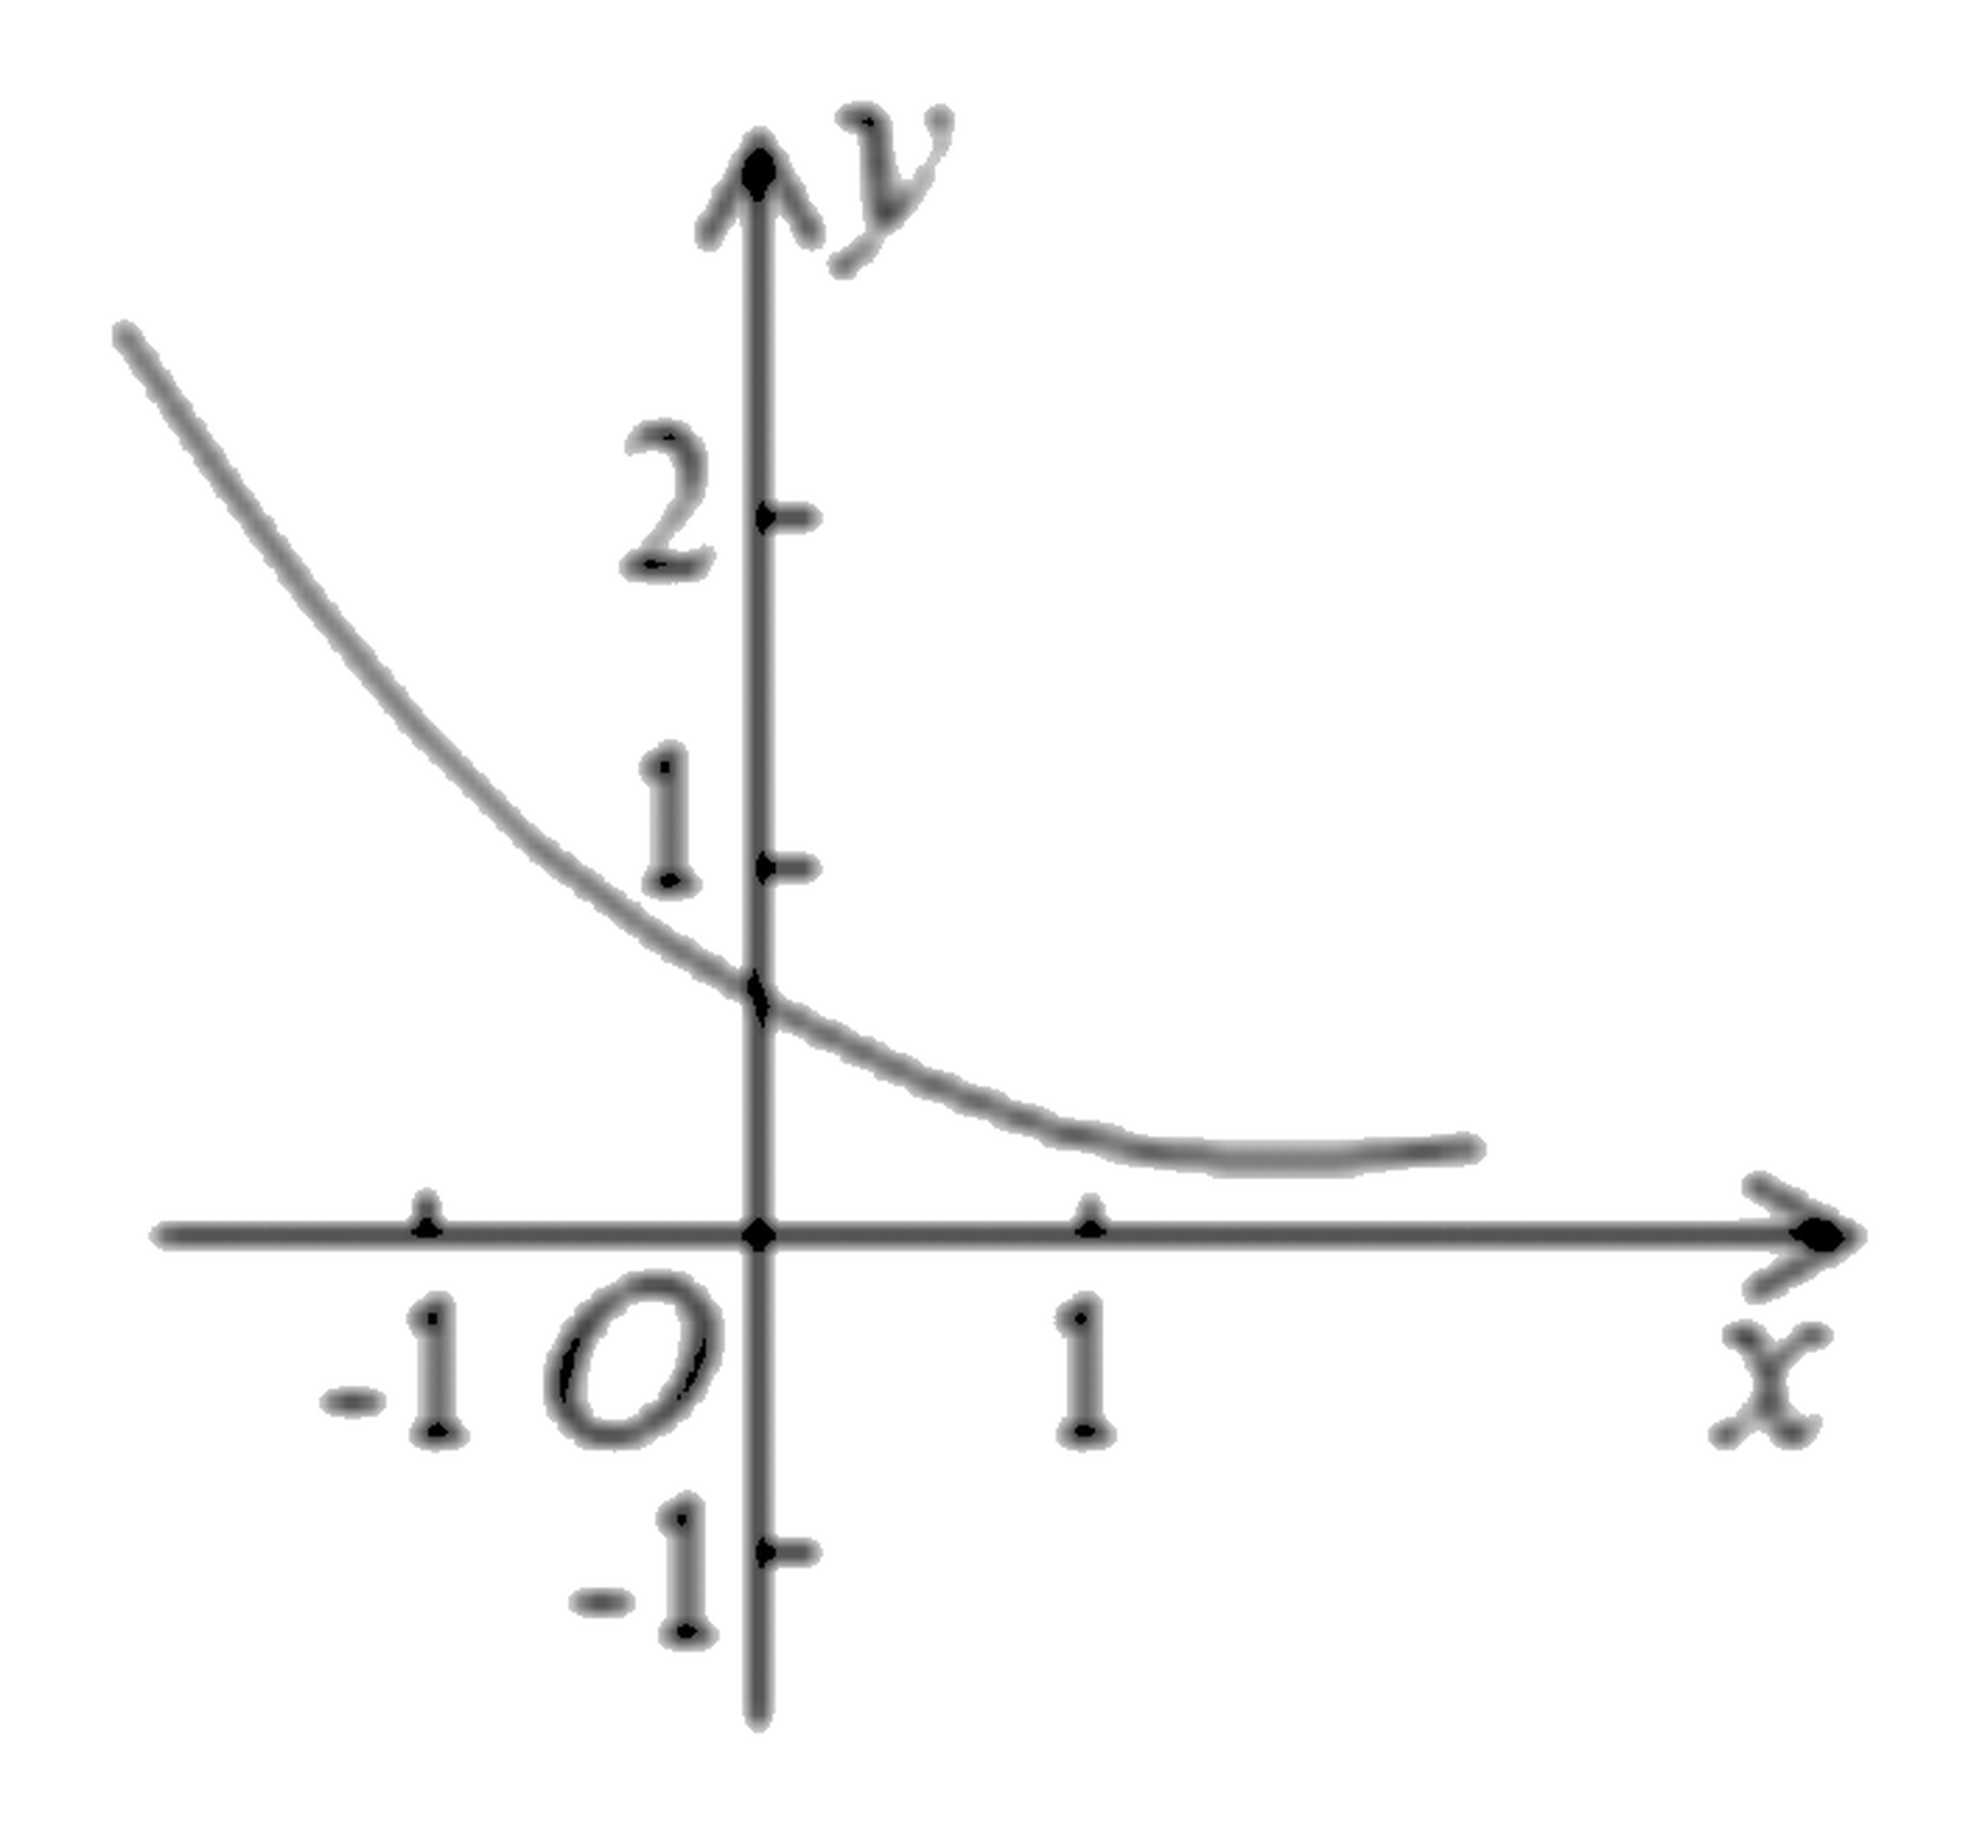
\includegraphics[width=0.30\textwidth]{figures/gao147_q15.png}
\end{center}

\ifanswer
\solbegin
\step{由图象从左到右下降得 $0<a<1$；}
\step{由图象与 $y$ 轴的交点得 $0<a^{-b}<1$，故 $b<0$；}
\step{故 $0<a<1$，$b<0$；故选 $D$.}
\solend
\fi

% === Q16 ===：位数新定义题（无弯引号，放大 04 页 z/q16_stem.png 确认）；四选项横排一行；解析 3 个印刷行
\item 数学运算是指在明晰运算对象的基础上，依据运算法则解决数学问题的素养. 因为运算，数的威力无限；没有运算，数就只是一个符号，对数运算与指数运算是两类重要的运算，对数的运算性质降低了运算的级别，简化了运算，在数学发展史上是伟大的成就. 而位数是指一个自然数有效位的个数，例如：$2^{10}=1024$，所以 $2^{10}$ 的位数为 4. 请你运用所学过的对数运算的知识，估计 $2025^{2026}$ 的位数是\mbox{（\quad）}

\keepwithprev
A. 6697\qquad B. 6698\qquad C. 6699\qquad D. 6700

\ifanswer
\solbegin
\step{设 $2025^{2026}=t$，所以 $\lg t=2026\lg2025$，}
\step{因为 $\lg2025\approx3.3064$，所以 $\lg t\approx6698.8$，}
\step{所以 $t\approx10^{6698.8}\in(10^{6698},10^{6699})$，所以 $2025^{2026}$ 的位数为 6699. 故选 $C$.}
\solend
\fi

\end{enumerate}

\bigsec{三、解答题}

\begin{enumerate}
\setcounter{enumi}{16}

% === Q17 ===：题干＋解析均在 04 页；集合描述竖线 \mid、描述内半角逗号照录；
% 空集 \varnothing、子集 \subseteq（放大 04 页 z/subset_04_q17b.png 确认带下划线）、数集 \R；
% 解析 5 个印刷行，首行末"所以 A=(-∞,-2)∪(3,+∞)"原卷无标点，照录不补
\item 已知集合 $A=\left\{x\mid \dfrac{x+2}{x-3}>0,x\in\R\right\}$，$B=\{x\mid \lvert x-2a\rvert\leqslant2,x\in\R\}$.

(1) 若 $a=1$，求 $A\cap B$；

(2) 若 $A\cap B=\varnothing$，求实数 $a$ 的取值范围.

\ifanswer
\solbegin
\step{由 $\dfrac{x+2}{x-3}>0$，得 $x<-2$ 或 $x>3$，所以 $A=(-\infty,-2)\cup(3,+\infty)$}
\step{(1) 当 $a=1$ 时，$B=\{x\mid \lvert x-2\rvert\leqslant2\}=[0,4]$，于是 $A\cap B=(3,4]$；}
\step{(2) $B=[2a-2,2a+2]$，}
\step{则 $A\cap B=\varnothing\Leftrightarrow[2a-2,2a+2]\subseteq[-2,3]\Leftrightarrow\begin{cases}2a-2\geqslant-2\\2a+2\leqslant3\end{cases}\Leftrightarrow0\leqslant a\leqslant\dfrac{1}{2}$，}
\step{所以实数 $a$ 的取值范围为 $\left[0,\dfrac{1}{2}\right]$.}
\solend
\fi

% === Q18 ===：氟化物／臭氧应用题；"氟化物""（如冰箱等）"全角夹注照录（放大 05 页 z/q18_line1.png 确认）；
% 关系式 $Q=Q_0e^{-0.0025t}$ 原卷独立一行，按一段照录；解析 6 个印刷行
\item 有些家用电器（如冰箱等）使用了氟化物，氟化物的释放破坏了大气上层的臭氧层，使臭氧含量 $Q$ 呈指数函数型变化，在氟化物排放量维持某种水平时，具有关系式

$Q=Q_0e^{-0.0025t}$，其中 $Q_0$ 是臭氧的初始量.

(1) 随时间 $t$ 的增加，臭氧的含量是增加还是减少？

(2) 试估计多少年以后将会有一半的臭氧消失.（用计算器计算）

\ifanswer
\solbegin
\step{(1) 对于函数 $Q=Q_0e^{-0.0025t}$，显然 $Q>0$，}
\step{任取 $t_1$、$t_2\in(0,+\infty)$，且 $t_1<t_2$，则 $t_2-t_1>0$，}
\step{所以 $\dfrac{Q_1}{Q_2}=\dfrac{Q_0e^{-0.0025t_1}}{Q_0e^{-0.0025t_2}}=e^{-0.0025(t_1-t_2)}=e^{0.0025(t_2-t_1)}>e^0=1$，所以 $Q_1>Q_2$，}
\step{故随着时间 $t$ 的增加，臭氧的含量是减少的；}
\step{(2) 令 $\dfrac{Q}{Q_0}=\dfrac{1}{2}$，即 $\dfrac{Q_0e^{-0.0025t}}{Q_0}=e^{-0.0025t}=\dfrac{1}{2}$，得 $-0.0025t=\ln\dfrac{1}{2}\approx-0.6931$，}
\step{解得 $t\approx277$，故估计 277 年以后将会有一半的臭氧消失.}
\solend
\fi

% === Q19 ===：题干用"图像"、解析两处用"图象"逐处照录不统一（05 页）；数集 \Z；
% 题干＋解析前 4 行在 05 页、解析后 3 行在 06 页；解析共 7 个印刷行
\item 已知幂函数 $f(x)=x^{-m^2+4m}(m\in\Z)$ 的图像关于 $y$ 轴对称，且在区间 $(0,+\infty)$ 上是严格增函数.

(1) 求 $m$ 的值；

(2) 求满足不等式 $(2a+1)^m<(a+1)^m$ 的实数 $a$ 的取值范围.

\ifanswer
\solbegin
\step{(1) 由题意得 $-m^2+4m>0$，解得 $0<m<4$，}
\step{因为 $m\in\Z$，所以 $m=1$ 或 $m=2$ 或 $m=3$.}
\step{当 $m=1$ 或 $m=3$ 时，$f(x)=x^3$，图象关于原点对称，不合题意；}
\step{当 $m=2$ 时，$f(x)=x^4$，图象关于 $y$ 轴对称，符合题意，所以 $m=2$.}
\step{(2) 代入 $m=2$，不等式为 $(2a+1)^2<(a+1)^2$，}
\step{得 $(2a+1)^2-(a+1)^2=a(3a+2)<0$，因此 $-\dfrac{2}{3}<a<0$，}
\step{所求范围为 $\left(-\dfrac{2}{3},0\right)$.}
\solend
\fi

% === Q20 ===：指数函数题，题干用"图像"；(3) 长求和式（分数 1/2026、1011/2026、2011/2026、
% 15/2026、1015/2026、2025/2026 放大 06 页 z/q20_sum_06a.png 确认）；题干在 06 页、
% 解析前 6 行在 06 页下半、后 6 行在 07 页上半；解析共 12 个印刷行
\item 已知指数函数 $y=a^x$（$a>0,a\ne1$）的图像经过点 $(1,4)$.

(1) 求实数 $a$ 的值；

(2) 若 $f(x)=(a^x)^2-2\cdot a^x-8$，当 $x\in\R$ 时，不等式 $f(x)>m\cdot4^x-12$ 恒成立，求 $m$ 的取值范围；

(3) 记 $g(x)=\dfrac{1}{a^x+2}$，求证：$g(x)+g(1-x)$ 为定值，并求 $g(0)+g\left(\dfrac{1}{2026}\right)+g\left(\dfrac{1011}{2026}\right)+g\left(\dfrac{2011}{2026}\right)+g\left(\dfrac{1}{2}\right)+g\left(\dfrac{15}{2026}\right)+g\left(\dfrac{1015}{2026}\right)+g\left(\dfrac{2025}{2026}\right)+g(1)$ 的值.

\ifanswer
\solbegin
\step{(1) 将 $(1,4)$ 代入 $y=a^x$，得 $a^1=4$，即 $a=4$.}
\step{(2) 令 $t=4^x$，当 $x\in\R$ 时，$t$ 取遍所有正实数.}
\step{原不等式等价于 $t^2-2t-8>mt-12\Leftrightarrow m<t+\dfrac{4}{t}-2$，}
\step{由基本不等式，$t+\dfrac{4}{t}-2\geqslant2\sqrt{t\cdot\dfrac{4}{t}}-2=2$，}
\step{当且仅当 $t=\dfrac{4}{t}$，即 $t=2$ 时取等号，}
\step{因此原不等式恒成立的充要条件为 $m<2$，即 $m\in(-\infty,2)$.}
\step{(3) 对任意 $x\in\R$，令 $t=4^x>0$，则 $4^{1-x}=\dfrac{4}{t}$，}
\step{从而 $g(x)+g(1-x)=\dfrac{1}{t+2}+\dfrac{1}{\dfrac{4}{t}+2}=\dfrac{1}{t+2}+\dfrac{t}{2(t+2)}=\dfrac{1}{2}$，}
\step{因此 $g(x)+g(1-x)$ 为定值 $\dfrac{1}{2}$.}
\step{原式中，0 与 1、$\dfrac{1}{2026}$ 与 $\dfrac{2025}{2026}$、$\dfrac{1011}{2026}$ 与 $\dfrac{1015}{2026}$、$\dfrac{2011}{2026}$ 与 $\dfrac{15}{2026}$}
\step{分别配对，每对函数值之和均为 $\dfrac{1}{2}$，且 $g\left(\dfrac{1}{2}\right)=\dfrac{1}{4^{\frac12}+2}=\dfrac{1}{4}$，}
\step{所以所求和为 $4\cdot\dfrac{1}{2}+\dfrac{1}{4}=\dfrac{9}{4}$.}
\solend
\fi

% === Q21 ===：不动点新定义题；题干在 07 页、解析续 08／09 页，共 20 个印刷行；
% 判别式两形混用：08 页 (2) cases 内等腰偏高 \Delta、09 页 (3) 扁等边 \triangle，逐处照录不统一
% （放大 /tmp/gao147/z/delta_vs_triangle.png 并排确认）；数集 \R；\forall 照录；
% 第 6—8 行是原卷一个长算式折成的三个印刷行，按印刷行分三条 \step、不并折行
\item 对于二次函数 $y=mx^2+nx+t(m\ne0)$，若存在 $x_0\in\R$，使得 $mx_0^2+nx_0+t=x_0$ 成立，则称 $x_0$ 为二次函数 $y=mx^2+nx+t(m\ne0)$ 的不动点.

(1) 求二次函数 $y=x^2-x-3$ 的不动点；

(2) 若二次函数 $y=2x^2-(3+a)x+a-1$ 有两个不相等的不动点 $x_1$、$x_2$，且 $x_1$、$x_2>0$，求 $\dfrac{x_1}{x_2}+\dfrac{x_2}{x_1}$ 的最小值；

(3) 若对任意实数 $b$，二次函数 $y=ax^2+(b+1)x+(b-1)(a\ne0)$ 恒有不动点，求 $a$ 的取值范围.

\ifanswer
\solbegin
\step{(1) 令 $x^2-x-3=x$，即 $x^2-2x-3=0$，即 $(x-3)(x+1)=0$，}
\step{解得 $x_1=-1$，$x_2=3$，所以不动点为 $-1$ 和 $3$.}
\step{(2) 由题意，$2x^2-(3+a)x+a-1=x$ 有两个不相等的正实数根，}
\step{即方程 $2x^2-(4+a)x+a-1=0$ 有两个不相等的正实数根，}
\step{所以 $\begin{cases}\Delta=(4+a)^2-8(a-1)>0\\x_1+x_2=\dfrac{4+a}{2}>0\\x_1\cdot x_2=\dfrac{a-1}{2}>0\end{cases}$，解得 $a>1$，}% 判别式原卷印等腰偏高粗三角 $\Delta$（放大 08 页 z/delta_08_q21cases.png）
\step{所以 $\dfrac{x_1}{x_2}+\dfrac{x_2}{x_1}=\dfrac{x_1^2+x_2^2}{x_1\cdot x_2}=\dfrac{(x_1+x_2)^2-2x_1\cdot x_2}{x_1\cdot x_2}=\dfrac{(x_1+x_2)^2}{x_1\cdot x_2}-2$}
\step{$=\dfrac{\left(\dfrac{4+a}{2}\right)^2}{\dfrac{a-1}{2}}-2=\dfrac{\dfrac{(a+4)^2}{4}}{\dfrac{a-1}{2}}-2=\dfrac{(a-1+5)^2}{2(a-1)}-2$}
\step{$=\dfrac{(a-1)^2+10(a-1)+25}{2(a-1)}-2=\dfrac{a-1}{2}+\dfrac{25}{2(a-1)}+3$.}
\step{因为 $a>1$，所以 $a-1>0$，}
\step{所以 $\dfrac{a-1}{2}+\dfrac{25}{2(a-1)}+3\geqslant2\sqrt{\dfrac{a-1}{2}\cdot\dfrac{25}{2(a-1)}}+3=8$，}
\step{当且仅当 $\dfrac{a-1}{2}=\dfrac{25}{2(a-1)}$，即 $a=6$ 时等号成立，}
\step{所以 $\dfrac{x_1}{x_2}+\dfrac{x_2}{x_1}$ 的最小值为 $8$.}
\step{(3) 设 $f(x)=ax^2+(b+1)x+b-1$，}
\step{则方程 $f(x)=x$，可化为 $ax^2+(b+1)x+b-1=x$，}
\step{即 $ax^2+bx+b-1=0$，}
\step{由题意得一元二次方程 $ax^2+bx+b-1=0$ 有解，又 $a\ne0$，}
\step{所以方程 $ax^2+bx+b-1=0$ 的判别式 $\triangle=b^2-4a(b-1)\geqslant0$，}% 判别式原卷印扁等边细线三角 $\triangle$（放大 09 页 z/triangle_09_q21.png），与 (2) 高 $\Delta$ 混用、照录不统一
\step{即 $b^2-4ab+4a\geqslant0$，则该不等式对 $\forall b\in\R$ 恒成立，}
\step{则 $(4a)^2-4\times4a\leqslant0$，且 $a\ne0$，解得 $0<a\leqslant1$，}
\step{所以实数 $a$ 的取值范围是 $(0,1]$.}
\solend
\fi

\end{enumerate}

\end{document}
"
%
% ① 原始材料：微信公众号"魔都数学加油站"文章，连载"27学年高一147"，原文标题
% "27学年高一147——2026-2027年上海市华师大三附中高一上期中"；
% 原文链接：https://mp.weixin.qq.com/s/X_gPW1JWoTAl2Bky_xEEGw 。
% 正文为 9 张 PNG 页（01/06/08/09 为 2560×3620，02/03/04/05/07 为 4762×6735，
% 同一篇各页分辨率混排，逐页按各自分辨率裁图核对，别按预览比例换算裁框）。
% 体例：混合体例讲评版——19 题中 Q4/Q5/Q7/Q9 只印【答案】、无【解析】，其余 15 题印
% 【解析】（逐题核实，见 ② ②）。题目、答案、解析均据原图转录；卷面粉红色水印
% "魔都数学加油站"及公众号页脚未录入。
% 全卷插图清单（逐页通读 9 页确认）：仅 1 处题目配图——
%   · Q15 递减指数函数小坐标系（03 页右侧：坐标轴、y 轴刻度 2/1/-1、x 轴刻度 -1/1、
%     原点 O、x/y 轴标），为"图像如图所示"的题目配图（选择题选项旁），三版都出；
%     裁自 03 页去粉色水印、去色、4× LANCZOS 放大存 figures/gao147_q15.png；
%   其余 8 页逐页确认无其它题目配图、无【解析】内配图、无表格，
%   亦无"题干写如图而源码漏图"一处；Q12/Q17/Q21 的 cases 块为数学块（非图）。
%
% 卷首标题：原卷印作"2026-2027 年华师大三附中高一上期中"，年份区间按全稿惯例排 en dash；
% 原卷卷面未印副标题，本稿按同期中卷（高一140／141／143／144／145／146）知识模块口径
% 补出"集合与常用逻辑用语、不等式、函数"。
%
% 题号体例（逐页核实定稿）：本卷共 19 题——一、填空题 3—12（10 题）、
% 二、选择题 13—16（4 题）、三、解答题 17—21（5 题）。
% 三节分别 \setcounter{enumi}{2}／{12}／{16}。原卷从第 3 题起、无第 1、2 题，
% 本稿保留原题号；全卷无附加题节（Q21 解析末行"所以实数 a 的取值范围是 (0,1]."
% 为全卷收尾，09 页下半仅水印、无正文）。
%
% ② 与原卷的排版差异：
%   ① 原文从第 3 题起，本稿保留原题号；共 19 题三节；
%   ② 混合体例：原卷 Q4/Q5/Q7/Q9 只印【答案】、无【解析】（分别为 a≤0、(-1,2)、
%      真、(-∞,1)），按 高一140 第 5 题／高一145 Q3 成例提 \ans{}、不补造解析；
%      其余 15 题印【解析】，用 \solbegin…\solend，选择题答案在解析末句"故选 X"
%      （Q13 选 B、Q14 选 B、Q15 选 D、Q16 选 C，逐个放大原图核实）、题干括号
%      \mbox{（\quad）} 留空、不另提 \ans{}；填空／解答答案落在解析里；
%      答案版【答案】/【解析】标记数 = 19（4 个 \ans ＋ 15 个 \solbegin）= 全卷题数；
%   ③ 原卷卷面未印副标题，本稿按知识模块口径补出；
%   ④ 原卷填空横线按全稿惯例排 \blankline[4.4em]；选择题括号排 \mbox{（\quad）}、
%      选项段前按惯例加 \keepwithprev；Q14／Q15 四选项为 2×2 两印刷行（A/B 一行、
%      C/D 一行），用空行分段照录（非一行 \qquad、亦非竖排四行）；解答题不留作答区、
%      不加 \anspace（原卷为讲评版，与 129／131／132／133／136／140／141／143／144／145／146 同）；
%   ⑤ 数集：Q4"A∪B=R"、Q13"f(x)=x^3 在 R 上严格增"、Q17"x∈R"两处、
%      Q20"x∈R"两处、Q21"x_0∈R""∀b∈R"原卷印斜体或黑板粗体 R，按全稿惯例统一改 \R；
%      Q19"m∈Z"改 \Z；本卷未出现 N（\N^* 无对应处）。绝对值排 \lvert…\rvert，
%      集合描述竖线排 \mid；不等号按全稿惯例排 \leqslant／\geqslant（原卷印 \le／\ge 形，
%      【答案】a≤0 亦排 \leqslant）；空集 \varnothing（Q17 两处）；
%      子集 \subseteq（Q17 带下划线，放大 04 页确认）；本卷未出现 \subset／\subsetneq，
%      亦未出现补集上划线 \overline{}；\left…\right 不得拆到不同 $…$ 组；
%   ⑥ 子题标号 (1)(2)(3) 半角括号照录；cases 块整体算一个印刷行（Q3、Q12 一行内
%      两个 cases、Q17、Q21(2)）；本卷解析内无圈数字①②③（无 \text{①} 需求）；
%      数学式内 CJK 用 \text{}（本卷未见）；
%   ⑦ 题干中的中文弯引号按原卷照录：Q7 命题"若 A∪B=B，则 A∩B=A"与
%      (填 " 真 " 或 " 假 ")、Q10 (填 ">" "<" "≤" "或≥")，含引号内空格；
%      注释内一律 ASCII 引号；Q16 位数新定义题逐字放大确认无弯引号
%      （交办提示的"Q16 新定义题"举例未在本卷出现），未补造引号；
%   ⑧ 半角逗号在数学组之间是全稿惯例、非笔误（Q4"$A=(-\infty,0],B=[a,+\infty)$"、
%      Q5"$(a>0,a\ne1)$"、Q17 集合描述内"$>0,x\in R$""$\leqslant2,x\in R$"、
%      Q20 题干"$(a>0,a\ne1)$"、Q21"$y=mx^2+nx+t(m\ne0)$"等），逐处照录别改全角；
%      行末西文句点照录为 ASCII `.`；行中全角逗号／顿号照录；
%      Q7／Q10"(填…)"为半角括号、Q18"（如冰箱等）"为全角括号，逐处照录不统一；
%   ⑨ "图像／图象"逐处照录不统一：题干 5 处用"图像"（Q5"图像恒过定点"、
%      Q9"图像位于直线 y=x 的下方"、Q15"的图像如图所示"、Q19"的图像关于 y 轴对称"、
%      Q20"的图像经过点"），解析 4 处用"图象"（Q15"由图象从左到右下降"
%      "由图象与 y 轴的交点"、Q19"图象关于原点对称""图象关于 y 轴对称"），逐处核、不统一；
%   ⑩ 判别式 Δ/△ 混用是照录项：Q21(2) 解析 cases 块"Δ=(4+a)²−8(a−1)>0"
%      印等腰偏高粗三角 \Delta，Q21(3) 解析"判别式△=b²−4a(b−1)≥0"
%      印扁等边细线三角 \triangle，逐处放大判断、照录不得统一
%      （参照 高一142／144／145 头注④口径，详见 ④）；
%   ⑪ 一条 \step = 原卷解析的一个印刷行，cases 块整体算一个印刷行；别把原卷折行
%      并起来、别把一行拆多条。Q10 七行（跨 01→02 页）、Q12 七行（含一行两 cases）、
%      Q20 十二行（含"原式中…2011/2026 与 15/2026／分别配对…"折行两行）、
%      Q21 二十行（含第 6—8 行一个长算式折成三印刷行、含 cases）均按印刷行逐条断，
%      不丢行；
%   ⑫ 配图：逐页通读 9 页确认全卷仅 Q15 一处题目配图（见 ①），三版都出、
%      \includegraphics[width=0.30\textwidth]；图块较小，未加 \needvspace 大图块守卫
%      （仅 \bigsec 自带 \needvspace{3\baselineskip}）；三版切页审计均"合计异常：无"；
%   ⑬ 跨页续印按题合并：Q3—Q9 在 01 页（Q10 题干在 01 页末、解析首行亦在 01 页末）；
%      Q10 解析续 02 页 6 行、Q11 在 02 页、Q12 题干＋解析前 4 行在 02 页
%      （解析续 03 页 3 行）；"二、选择题"标题与 Q13、Q14、Q15 题干＋解析前 2 行在 03 页
%      （Q15 配图在 03 页右侧）；Q15 解析末行与 Q16、"三、解答题"标题、Q17 在 04 页；
%      Q18 在 05 页、Q19 题干＋解析前 4 行在 05 页（解析续 06 页 3 行）；
%      Q20 题干＋解析前 6 行在 06 页（解析续 07 页 6 行）、Q21 题干＋解析前 3 行在 07 页；
%      Q21 解析续 08 页 13 行、续 09 页 4 行（09 页下半仅水印、无正文）。
%      本稿按题连排，不丢行、不并折行；
%   ⑭ 原卷解析内无红色"法一／法二"之类小标题，故本卷无 \stepm；
%      水印"魔都数学加油站"红色不录入。
%
% ③ 行数复核：一条 \step／\stepm = 原卷解析的一个印刷行，cases 块作一个印刷行计。
%   逐题数（主会话逐页核对定稿）：Q3：1；Q4：0（只印【答案】、提 \ans{}，不计入 \step 账）；
%   Q5：0；Q6：1；Q7：0；Q8：2；Q9：0；Q10：7；Q11：4；Q12：7；Q13：6；Q14：4；
%   Q15：3；Q16：3；Q17：5；Q18：6；Q19：7；Q20：12；Q21：20。
%   合计 88 条 \step（本卷无 \stepm：解析内无红色"法一／法二"类小标题），
%   与原卷逐题印刷行相等。全卷 15 题设 \solbegin…\solend ＋ 4 题一处 \ans{}，
%   答案版【答案】/【解析】标记数 = 19 = 全卷题数。
%
% ④ 判别式／子集符号结论（逐处放大原图照录、不得统一，主会话像素级复核）：
%   判别式全卷 2 处、两形混用逐处照录不统一（参照 高一142／144 头注④口径）：
%     · Q21(2) 解析 cases 块"Δ=(4+a)²−8(a−1)>0" 原卷印等腰偏高粗三角
%       （高>宽、粗笔画），照录 \Delta（放大 08 页 /tmp/gao147/z/delta_08_q21cases.png
%       与 z/delta_vs_triangle.png 左图确认）；
%     · Q21(3) 解析"判别式△=b²−4a(b−1)≥0" 原卷印扁等边细线三角
%       （宽≈高、细线），照录 \triangle（放大 09 页 /tmp/gao147/z/triangle_09_q21.png
%       与 z/delta_vs_triangle.png 右图并排确认）。
%   子集／补集：Q17 解析"[2a−2,2a+2]⊆[−2,3]" 原卷印带下划线 ⊆，照录 \subseteq
%     （放大 04 页 /tmp/gao147/z/subset_04_q17b.png 确认）；Q17"A∩B=∅"空集 \varnothing；
%     集合描述竖线 \mid（Q10 M、Q12 解集、Q17 A/B）；并集 \cup（Q4、Q17）、
%     交集 \cap（Q7、Q17）、不属于 \notin（Q10）；数集 \R／\Z 归一见 ② ⑤。
%   本卷未出现 \subset／\subsetneq，未出现补集上划线 \overline{}。
%
% ⑤ 存疑照录（放大原图确认，照录未改、正文对应处另有 % 注）：
%   1. Q4/Q5/Q7/Q9 只印【答案】、无【解析】，按成例提 \ans{}、不补造解析
%      （混合体例逐题核实，见 ② ②）。
%   2. Q21(2) 判别式高 \Delta 与 Q21(3) 判别式扁 \triangle 两形混用，
%      逐处照录不统一（见 ④）。
%   3. "图像／图象"题干 5 处"图像"、解析 4 处"图象"，逐处照录不统一（见 ② ⑨）。
%   4. Q7／Q10"(填…)"半角括号与 Q18"（如冰箱等）"全角括号，逐处照录不统一。
%   5. Q16 位数新定义题逐字放大确认无弯引号（交办提示的"Q16 新定义题"举例
%      未在本卷出现），未补造引号；全卷弯引号仅 Q7、Q10 两处。
%   6. Q17 解析首行末"所以 A=(-∞,-2)∪(3,+∞)"、Q20(3) 解析"…2011/2026 与 15/2026"
%      行末原卷均无标点，照录未补；Q21(2) 第 6—8 行一个长算式折成三印刷行，
%      按印刷行分三条 \step、不并折行。
%   全卷除此 6 类外未发现其它笔误／自相矛盾处。
%
% ⑥ 跨页续印按题合并说明：见 ② ⑬。
%
\documentclass[a4paper,11pt]{article}
\usepackage{common}

\begin{document}

\examtitlest[3]{2026--2027 年华师大三附中高一上期中}{集合与常用逻辑用语、不等式、函数}

\bigsec{一、填空题}

\begin{enumerate}
\setcounter{enumi}{2}

% === Q3 ===：印【解析】，1 个印刷行（cases 块整体算一行）
\item 函数 $y=(a^2-5a+7)a^x+6-2a$ 是指数函数，则 $a$ 的值为\blankline[4.4em].

\ifanswer
\solbegin
\step{由题意得 $\begin{cases}a^2-5a+7=1\\6-2a=0\end{cases}$，解得 $a=3$.}
\solend
\fi

% === Q4 ===：原卷只印【答案】、无【解析】，按 高一140 第 5 题／高一145 Q3 成例提 \ans{}、不补造解析；
% 题干数学组内半角逗号 $A=(-\infty,0],B=[a,+\infty)$ 照录（放大 01 页 z/q4_stem.png 确认）
\item 已知 $A=(-\infty,0],B=[a,+\infty)$，且 $A\cup B=\R$，则实数 $a$ 的取值范围为\blankline[4.4em].

\ifanswer
\ans{$a\leqslant0$}
\fi

% === Q5 ===：只印【答案】；题干"图像"照录（放大 01 页 z/q5_stem.png 确认）；
% 数学组内半角逗号 $(a>0,a\ne1)$ 照录
\item 函数 $y=a^{x+1}+1(a>0,a\ne1)$ 的图像恒过定点\blankline[4.4em].

\ifanswer
\ans{$(-1,2)$}
\fi

% === Q6 ===：印【解析】，1 个印刷行
\item 已知方程 $x^2+2x-4=0$ 的两个根为 $x_1$、$x_2$，则 $x_1^2+x_2^2$ 的值为\blankline[4.4em].

\ifanswer
\solbegin
\step{$x_1^2+x_2^2=(x_1+x_2)^2-2x_1x_2=4+8=12$.}
\solend
\fi

% === Q7 ===：只印【答案】；中文弯引号"若 A∪B=B，则 A∩B=A"与(填 " 真 " 或 " 假 ")内的空格照录
% （放大 01 页 z/q7_quotes_7x.png、z/q7_tail.png 确认，括号为半角）
\item 命题 “若 $A\cup B=B$，则 $A\cap B=A$” 为\blankline[4.4em]命题(填 “ 真 ” 或 “ 假 ”).

\ifanswer
\ans{真}
\fi

% === Q8 ===：印【解析】，2 个印刷行；不等号按全稿惯例 \geqslant／\leqslant
\item 已知正实数 $a$、$b$ 满足 $a+4b=1$，则 $ab$ 的最大值为\blankline[4.4em].

\ifanswer
\solbegin
\step{$a+4b\geqslant2\sqrt{a\cdot4b}\Rightarrow ab\leqslant\dfrac{1}{16}$，当且仅当 $a=4b=\dfrac{1}{2}$ 时取等号，}
\step{则 $ab$ 的最大值为 $\dfrac{1}{16}$.}
\solend
\fi

% === Q9 ===：只印【答案】；题干"图像"照录（放大 01 页 hi_01_2 确认）
\item 若幂函数 $y=x^s$ 在 $x>1$ 时的图像位于直线 $y=x$ 的下方，则 $s$ 的取值范围是\blankline[4.4em].

\ifanswer
\ans{$(-\infty,1)$}
\fi

% === Q10 ===：印【解析】，共 7 个印刷行（题在 01 页末起 1 行、续 02 页 6 行）；
% 题干跨两印刷行"则 |ab|+1 ____ |a|+|b|（填…）"按一句连排；(填…)为半角括号、引号内空格照录
\item 已知不等式 $\lvert2x+1\rvert+\lvert2x-1\rvert<4$ 的解集为 $M$. 设实数 $a\in M$，$b\notin M$，则 $\lvert ab\rvert+1$\blankline[4.4em] $\lvert a\rvert+\lvert b\rvert$(填 “$>$”，“$<$”，“$\leqslant$” “或$\geqslant$”).

\ifanswer
\solbegin
\step{当 $x<-\dfrac{1}{2}$ 时，不等式化为 $-2x-1+1-2x<4$，即 $x>-1$，所以 $-1<x<-\dfrac{1}{2}$；}
\step{当 $-\dfrac{1}{2}\leqslant x\leqslant\dfrac{1}{2}$ 时，不等式化为 $2x+1-2x+1<4$，即 $2<4$，所以 $-\dfrac{1}{2}\leqslant x\leqslant\dfrac{1}{2}$；}
\step{当 $x>\dfrac{1}{2}$ 时，不等式化为 $2x+1+2x-1<4$，即 $x<1$，所以 $\dfrac{1}{2}<x<1$；}
\step{综上，$M=\{x\mid -1<x<1\}$.}
\step{因为 $a\in M$，$b\notin M$，所以 $\lvert a\rvert<1$，$\lvert b\rvert\geqslant1$.}
\step{而 $\lvert ab\rvert+1-(\lvert a\rvert+\lvert b\rvert)=\lvert ab\rvert+1-\lvert a\rvert-\lvert b\rvert=(\lvert a\rvert-1)(\lvert b\rvert-1)$，}
\step{所以 $\lvert ab\rvert+1\leqslant\lvert a\rvert+\lvert b\rvert$.}
\solend
\fi

% === Q11 ===：印【解析】，4 个印刷行（02 页）
\item 已知 $m>1$，$n>1$，$\lg m=\log_n100$，则 $mn$ 的最小值为\blankline[4.4em].

\ifanswer
\solbegin
\step{由 $m>1$，$n>1$，得 $\lg m>0$，$\lg n>0$，}
\step{因为 $\lg m=\log_n100=\dfrac{\lg100}{\lg n}=\dfrac{2}{\lg n}$，所以 $\lg m\cdot\lg n=2$，}
\step{所以 $\lg(mn)=\lg m+\lg n\geqslant2\sqrt{\lg m\cdot\lg n}=2\sqrt2$，}
\step{当且仅当 $m=n=10^{\sqrt2}$ 时取等号，则 $mn\geqslant10^{2\sqrt2}$，即 $mn$ 的最小值为 $10^{2\sqrt2}$.}
\solend
\fi

% === Q12 ===：印【解析】，共 7 个印刷行（02 页 4 行、03 页 3 行）；
% 第 3 行"则 [cases]，得 [cases]，"两个 cases 块同属一个印刷行，整体作一条 \step（照 高一146 Q11 成例）
\item 已知关于 $x$ 的不等式 $ax^2+bx+c\leqslant1$ 的解集为 $\{x\mid -1\leqslant x\leqslant3\}$. 若关于 $x$ 的不等式 $ax^2+(b-1)x+c-2\leqslant0$ 有且仅有 8 个整数解，则实数 $a$ 的取值范围是\blankline[4.4em].

\ifanswer
\solbegin
\step{由已知关于 $x$ 的不等式 $ax^2+bx+c\leqslant1$ 的解集为 $\{x\mid -1\leqslant x\leqslant3\}$，}
\step{得 $a>0$，且方程 $ax^2+bx+c-1=0$ 的两根分别为 $-1$ 和 $3$，}
\step{则 $\begin{cases}-1+3=-\dfrac{b}{a}\\-1\times3=\dfrac{c-1}{a}\end{cases}$，得 $\begin{cases}b=-2a\\c=1-3a\end{cases}$，}
\step{不等式 $ax^2+(b-1)x+c-2\leqslant0$ 等价于 $ax^2-(2a+1)x-(3a+1)\leqslant0$，}
\step{即 $\left[x-\left(3+\dfrac{1}{a}\right)\right](x+1)\leqslant0$，解得 $-1\leqslant x\leqslant3+\dfrac{1}{a}$，}
\step{因为关于 $x$ 的不等式 $ax^2+(b-1)x+c-2\leqslant0$ 有且仅有 8 个整数解，}
\step{因此 $6\leqslant3+\dfrac{1}{a}<7$，即 $3\leqslant\dfrac{1}{a}<4$，解得 $\dfrac{1}{4}<a\leqslant\dfrac{1}{3}$，所以 $a$ 的取值范围为 $\left(\dfrac{1}{4},\dfrac{1}{3}\right]$.}
\solend
\fi

\end{enumerate}

\bigsec{二、选择题}

\begin{enumerate}
\setcounter{enumi}{12}

% === Q13 ===：题干＋选项＋解析均在 03 页；四选项横排一行；解析 6 个印刷行，末句"故选 B."
\item $a<b<0$，则下列不等式能成立的是\mbox{（\quad）}

\keepwithprev
A. $\dfrac{a}{b}<1$\qquad B. $\lvert a\rvert>-b$\qquad C. $\dfrac{1}{a}<\dfrac{1}{b}$\qquad D. $b^3<a^3$

\ifanswer
\solbegin
\step{对于 $A$，令 $a=-4$，$b=-3$，满足 $a<b<0$，但 $\dfrac{a}{b}>1$，故 $A$ 错误，}
\step{对于 $B$，因为 $a<b<0$，所以 $-a>-b>0$，即 $\lvert a\rvert>-b$，故 $B$ 正确，}
\step{对于 $C$，令 $a=-4$，$b=-3$，满足 $a<b<0$，但 $\dfrac{1}{a}>\dfrac{1}{b}$，故 $C$ 错误，}
\step{对于 $D$，$f(x)=x^3$ 在 $\R$ 上严格增，因为 $a<b$，所以 $f(a)<f(b)$，}
\step{即 $a^3<b^3$，故 $D$ 错误.}
\step{故选 $B$.}
\solend
\fi

% === Q14 ===：四选项原卷为 2×2 两印刷行（A/B 一行、C/D 一行），用空行分段照录；解析 4 个印刷行
\item 已知 $a$、$b$ 为实数，若 $\alpha:ab=0$，$\beta:a^2+\sqrt{b}=0$，则 $\alpha$ 是 $\beta$ 的\mbox{（\quad）}

\keepwithprev
A. 充分不必要条件\qquad\qquad B. 必要不充分条件

C. 充要条件\qquad\qquad D. 既不充分也不必要条件

\ifanswer
\solbegin
\step{$\beta:a^2+\sqrt{b}=0$，所以 $a=0$ 且 $b=0$，}
\step{由 $a=0$，$b=0\Rightarrow ab=0$，反之不成立.}
\step{所以 $ab=0$ 是 $a=0$，$b=0$ 的必要不充分条件，即 $\alpha$ 是 $\beta$ 的必要不充分条件，}
\step{故选 $B$.}
\solend
\fi

% === Q15 ===：题目配图（03 页右侧小坐标系），三版都出；题干用"图像"、解析用"图象"逐处照录；
% 四选项 2×2 两印刷行；解析 3 个印刷行（03 页 2 行、04 页 1 行，末句"故选 D."与前行同一印刷行）
\item 函数 $f(x)=a^{x-b}$ 的图像如图所示，其中 $a$、$b$ 为常数，则下列结论正确的是\mbox{（\quad）}

\keepwithprev
A. $a>1$，$b<0$\qquad\qquad B. $a>1$，$b>0$

C. $0<a<1$，$b>0$\qquad\qquad D. $0<a<1$，$b<0$

\begin{center}
% 递减指数函数小坐标系图取 03 页右侧，去粉色水印、去色、4× LANCZOS 放大；题目配图三版都出
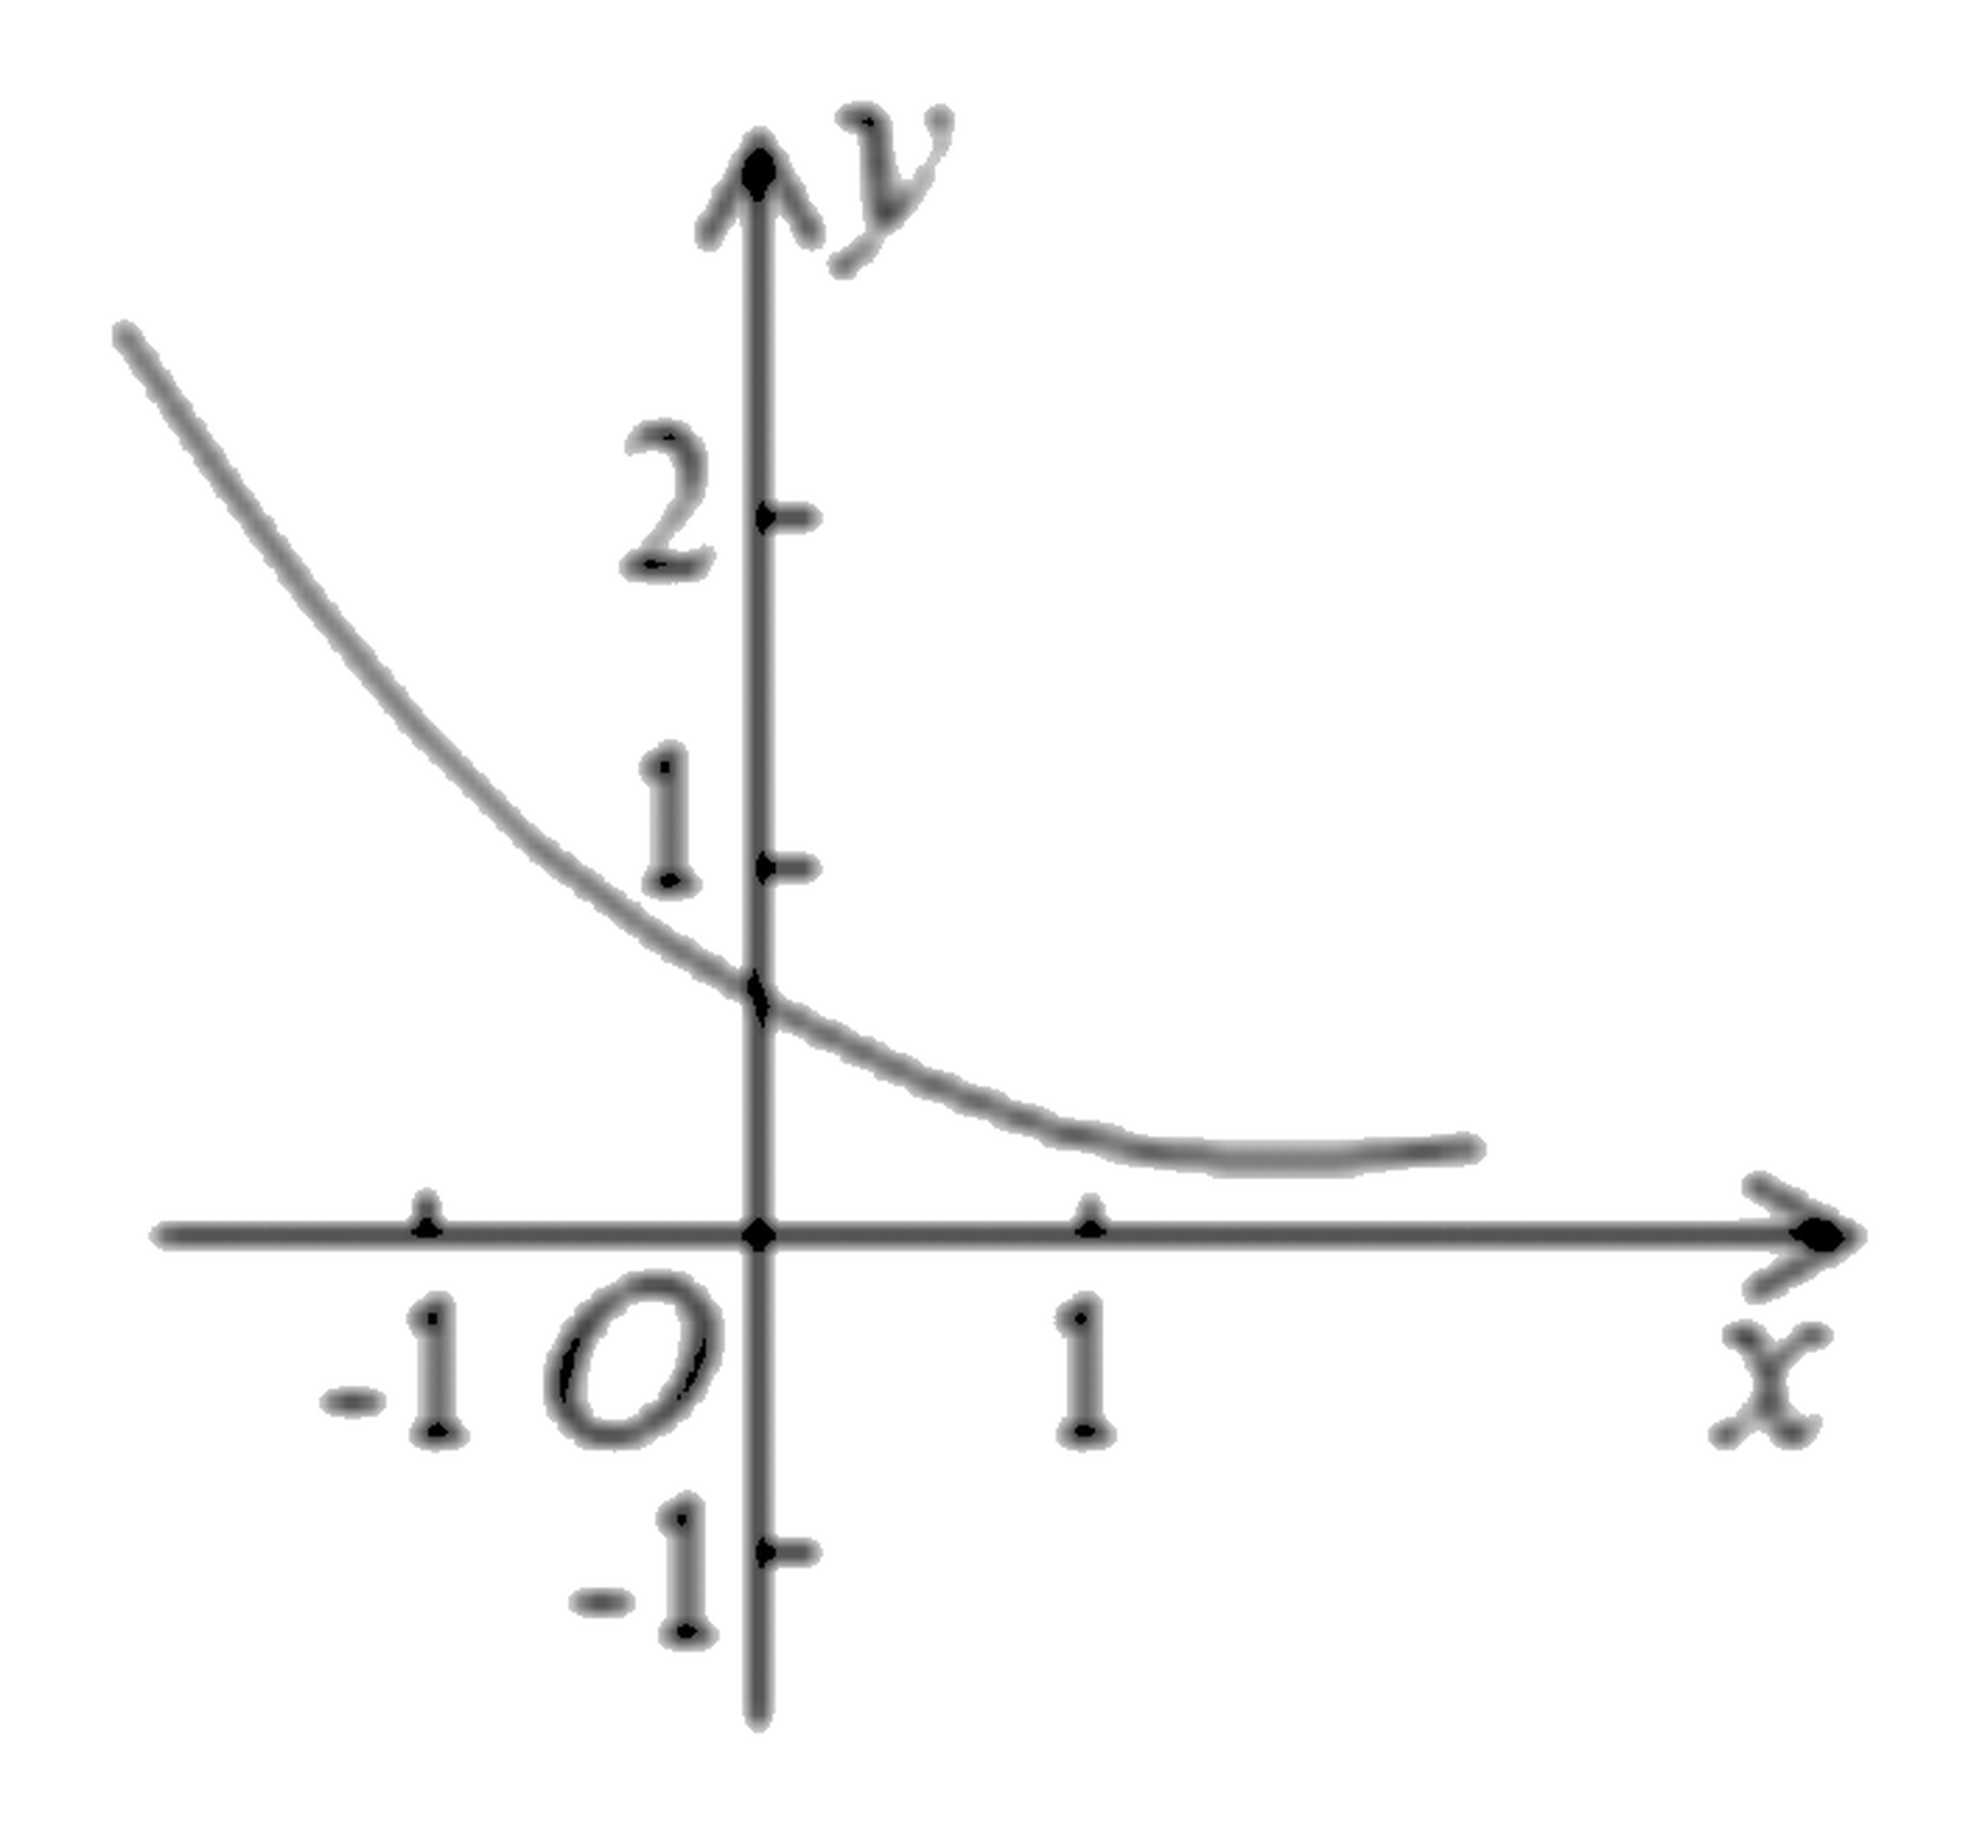
\includegraphics[width=0.30\textwidth]{figures/gao147_q15.png}
\end{center}

\ifanswer
\solbegin
\step{由图象从左到右下降得 $0<a<1$；}
\step{由图象与 $y$ 轴的交点得 $0<a^{-b}<1$，故 $b<0$；}
\step{故 $0<a<1$，$b<0$；故选 $D$.}
\solend
\fi

% === Q16 ===：位数新定义题（无弯引号，放大 04 页 z/q16_stem.png 确认）；四选项横排一行；解析 3 个印刷行
\item 数学运算是指在明晰运算对象的基础上，依据运算法则解决数学问题的素养. 因为运算，数的威力无限；没有运算，数就只是一个符号，对数运算与指数运算是两类重要的运算，对数的运算性质降低了运算的级别，简化了运算，在数学发展史上是伟大的成就. 而位数是指一个自然数有效位的个数，例如：$2^{10}=1024$，所以 $2^{10}$ 的位数为 4. 请你运用所学过的对数运算的知识，估计 $2025^{2026}$ 的位数是\mbox{（\quad）}

\keepwithprev
A. 6697\qquad B. 6698\qquad C. 6699\qquad D. 6700

\ifanswer
\solbegin
\step{设 $2025^{2026}=t$，所以 $\lg t=2026\lg2025$，}
\step{因为 $\lg2025\approx3.3064$，所以 $\lg t\approx6698.8$，}
\step{所以 $t\approx10^{6698.8}\in(10^{6698},10^{6699})$，所以 $2025^{2026}$ 的位数为 6699. 故选 $C$.}
\solend
\fi

\end{enumerate}

\bigsec{三、解答题}

\begin{enumerate}
\setcounter{enumi}{16}

% === Q17 ===：题干＋解析均在 04 页；集合描述竖线 \mid、描述内半角逗号照录；
% 空集 \varnothing、子集 \subseteq（放大 04 页 z/subset_04_q17b.png 确认带下划线）、数集 \R；
% 解析 5 个印刷行，首行末"所以 A=(-∞,-2)∪(3,+∞)"原卷无标点，照录不补
\item 已知集合 $A=\left\{x\mid \dfrac{x+2}{x-3}>0,x\in\R\right\}$，$B=\{x\mid \lvert x-2a\rvert\leqslant2,x\in\R\}$.

(1) 若 $a=1$，求 $A\cap B$；

(2) 若 $A\cap B=\varnothing$，求实数 $a$ 的取值范围.

\ifanswer
\solbegin
\step{由 $\dfrac{x+2}{x-3}>0$，得 $x<-2$ 或 $x>3$，所以 $A=(-\infty,-2)\cup(3,+\infty)$}
\step{(1) 当 $a=1$ 时，$B=\{x\mid \lvert x-2\rvert\leqslant2\}=[0,4]$，于是 $A\cap B=(3,4]$；}
\step{(2) $B=[2a-2,2a+2]$，}
\step{则 $A\cap B=\varnothing\Leftrightarrow[2a-2,2a+2]\subseteq[-2,3]\Leftrightarrow\begin{cases}2a-2\geqslant-2\\2a+2\leqslant3\end{cases}\Leftrightarrow0\leqslant a\leqslant\dfrac{1}{2}$，}
\step{所以实数 $a$ 的取值范围为 $\left[0,\dfrac{1}{2}\right]$.}
\solend
\fi

% === Q18 ===：氟化物／臭氧应用题；"氟化物""（如冰箱等）"全角夹注照录（放大 05 页 z/q18_line1.png 确认）；
% 关系式 $Q=Q_0e^{-0.0025t}$ 原卷独立一行，按一段照录；解析 6 个印刷行
\item 有些家用电器（如冰箱等）使用了氟化物，氟化物的释放破坏了大气上层的臭氧层，使臭氧含量 $Q$ 呈指数函数型变化，在氟化物排放量维持某种水平时，具有关系式

$Q=Q_0e^{-0.0025t}$，其中 $Q_0$ 是臭氧的初始量.

(1) 随时间 $t$ 的增加，臭氧的含量是增加还是减少？

(2) 试估计多少年以后将会有一半的臭氧消失.（用计算器计算）

\ifanswer
\solbegin
\step{(1) 对于函数 $Q=Q_0e^{-0.0025t}$，显然 $Q>0$，}
\step{任取 $t_1$、$t_2\in(0,+\infty)$，且 $t_1<t_2$，则 $t_2-t_1>0$，}
\step{所以 $\dfrac{Q_1}{Q_2}=\dfrac{Q_0e^{-0.0025t_1}}{Q_0e^{-0.0025t_2}}=e^{-0.0025(t_1-t_2)}=e^{0.0025(t_2-t_1)}>e^0=1$，所以 $Q_1>Q_2$，}
\step{故随着时间 $t$ 的增加，臭氧的含量是减少的；}
\step{(2) 令 $\dfrac{Q}{Q_0}=\dfrac{1}{2}$，即 $\dfrac{Q_0e^{-0.0025t}}{Q_0}=e^{-0.0025t}=\dfrac{1}{2}$，得 $-0.0025t=\ln\dfrac{1}{2}\approx-0.6931$，}
\step{解得 $t\approx277$，故估计 277 年以后将会有一半的臭氧消失.}
\solend
\fi

% === Q19 ===：题干用"图像"、解析两处用"图象"逐处照录不统一（05 页）；数集 \Z；
% 题干＋解析前 4 行在 05 页、解析后 3 行在 06 页；解析共 7 个印刷行
\item 已知幂函数 $f(x)=x^{-m^2+4m}(m\in\Z)$ 的图像关于 $y$ 轴对称，且在区间 $(0,+\infty)$ 上是严格增函数.

(1) 求 $m$ 的值；

(2) 求满足不等式 $(2a+1)^m<(a+1)^m$ 的实数 $a$ 的取值范围.

\ifanswer
\solbegin
\step{(1) 由题意得 $-m^2+4m>0$，解得 $0<m<4$，}
\step{因为 $m\in\Z$，所以 $m=1$ 或 $m=2$ 或 $m=3$.}
\step{当 $m=1$ 或 $m=3$ 时，$f(x)=x^3$，图象关于原点对称，不合题意；}
\step{当 $m=2$ 时，$f(x)=x^4$，图象关于 $y$ 轴对称，符合题意，所以 $m=2$.}
\step{(2) 代入 $m=2$，不等式为 $(2a+1)^2<(a+1)^2$，}
\step{得 $(2a+1)^2-(a+1)^2=a(3a+2)<0$，因此 $-\dfrac{2}{3}<a<0$，}
\step{所求范围为 $\left(-\dfrac{2}{3},0\right)$.}
\solend
\fi

% === Q20 ===：指数函数题，题干用"图像"；(3) 长求和式（分数 1/2026、1011/2026、2011/2026、
% 15/2026、1015/2026、2025/2026 放大 06 页 z/q20_sum_06a.png 确认）；题干在 06 页、
% 解析前 6 行在 06 页下半、后 6 行在 07 页上半；解析共 12 个印刷行
\item 已知指数函数 $y=a^x$（$a>0,a\ne1$）的图像经过点 $(1,4)$.

(1) 求实数 $a$ 的值；

(2) 若 $f(x)=(a^x)^2-2\cdot a^x-8$，当 $x\in\R$ 时，不等式 $f(x)>m\cdot4^x-12$ 恒成立，求 $m$ 的取值范围；

(3) 记 $g(x)=\dfrac{1}{a^x+2}$，求证：$g(x)+g(1-x)$ 为定值，并求 $g(0)+g\left(\dfrac{1}{2026}\right)+g\left(\dfrac{1011}{2026}\right)+g\left(\dfrac{2011}{2026}\right)+g\left(\dfrac{1}{2}\right)+g\left(\dfrac{15}{2026}\right)+g\left(\dfrac{1015}{2026}\right)+g\left(\dfrac{2025}{2026}\right)+g(1)$ 的值.

\ifanswer
\solbegin
\step{(1) 将 $(1,4)$ 代入 $y=a^x$，得 $a^1=4$，即 $a=4$.}
\step{(2) 令 $t=4^x$，当 $x\in\R$ 时，$t$ 取遍所有正实数.}
\step{原不等式等价于 $t^2-2t-8>mt-12\Leftrightarrow m<t+\dfrac{4}{t}-2$，}
\step{由基本不等式，$t+\dfrac{4}{t}-2\geqslant2\sqrt{t\cdot\dfrac{4}{t}}-2=2$，}
\step{当且仅当 $t=\dfrac{4}{t}$，即 $t=2$ 时取等号，}
\step{因此原不等式恒成立的充要条件为 $m<2$，即 $m\in(-\infty,2)$.}
\step{(3) 对任意 $x\in\R$，令 $t=4^x>0$，则 $4^{1-x}=\dfrac{4}{t}$，}
\step{从而 $g(x)+g(1-x)=\dfrac{1}{t+2}+\dfrac{1}{\dfrac{4}{t}+2}=\dfrac{1}{t+2}+\dfrac{t}{2(t+2)}=\dfrac{1}{2}$，}
\step{因此 $g(x)+g(1-x)$ 为定值 $\dfrac{1}{2}$.}
\step{原式中，0 与 1、$\dfrac{1}{2026}$ 与 $\dfrac{2025}{2026}$、$\dfrac{1011}{2026}$ 与 $\dfrac{1015}{2026}$、$\dfrac{2011}{2026}$ 与 $\dfrac{15}{2026}$}
\step{分别配对，每对函数值之和均为 $\dfrac{1}{2}$，且 $g\left(\dfrac{1}{2}\right)=\dfrac{1}{4^{\frac12}+2}=\dfrac{1}{4}$，}
\step{所以所求和为 $4\cdot\dfrac{1}{2}+\dfrac{1}{4}=\dfrac{9}{4}$.}
\solend
\fi

% === Q21 ===：不动点新定义题；题干在 07 页、解析续 08／09 页，共 20 个印刷行；
% 判别式两形混用：08 页 (2) cases 内等腰偏高 \Delta、09 页 (3) 扁等边 \triangle，逐处照录不统一
% （放大 /tmp/gao147/z/delta_vs_triangle.png 并排确认）；数集 \R；\forall 照录；
% 第 6—8 行是原卷一个长算式折成的三个印刷行，按印刷行分三条 \step、不并折行
\item 对于二次函数 $y=mx^2+nx+t(m\ne0)$，若存在 $x_0\in\R$，使得 $mx_0^2+nx_0+t=x_0$ 成立，则称 $x_0$ 为二次函数 $y=mx^2+nx+t(m\ne0)$ 的不动点.

(1) 求二次函数 $y=x^2-x-3$ 的不动点；

(2) 若二次函数 $y=2x^2-(3+a)x+a-1$ 有两个不相等的不动点 $x_1$、$x_2$，且 $x_1$、$x_2>0$，求 $\dfrac{x_1}{x_2}+\dfrac{x_2}{x_1}$ 的最小值；

(3) 若对任意实数 $b$，二次函数 $y=ax^2+(b+1)x+(b-1)(a\ne0)$ 恒有不动点，求 $a$ 的取值范围.

\ifanswer
\solbegin
\step{(1) 令 $x^2-x-3=x$，即 $x^2-2x-3=0$，即 $(x-3)(x+1)=0$，}
\step{解得 $x_1=-1$，$x_2=3$，所以不动点为 $-1$ 和 $3$.}
\step{(2) 由题意，$2x^2-(3+a)x+a-1=x$ 有两个不相等的正实数根，}
\step{即方程 $2x^2-(4+a)x+a-1=0$ 有两个不相等的正实数根，}
\step{所以 $\begin{cases}\Delta=(4+a)^2-8(a-1)>0\\x_1+x_2=\dfrac{4+a}{2}>0\\x_1\cdot x_2=\dfrac{a-1}{2}>0\end{cases}$，解得 $a>1$，}% 判别式原卷印等腰偏高粗三角 $\Delta$（放大 08 页 z/delta_08_q21cases.png）
\step{所以 $\dfrac{x_1}{x_2}+\dfrac{x_2}{x_1}=\dfrac{x_1^2+x_2^2}{x_1\cdot x_2}=\dfrac{(x_1+x_2)^2-2x_1\cdot x_2}{x_1\cdot x_2}=\dfrac{(x_1+x_2)^2}{x_1\cdot x_2}-2$}
\step{$=\dfrac{\left(\dfrac{4+a}{2}\right)^2}{\dfrac{a-1}{2}}-2=\dfrac{\dfrac{(a+4)^2}{4}}{\dfrac{a-1}{2}}-2=\dfrac{(a-1+5)^2}{2(a-1)}-2$}
\step{$=\dfrac{(a-1)^2+10(a-1)+25}{2(a-1)}-2=\dfrac{a-1}{2}+\dfrac{25}{2(a-1)}+3$.}
\step{因为 $a>1$，所以 $a-1>0$，}
\step{所以 $\dfrac{a-1}{2}+\dfrac{25}{2(a-1)}+3\geqslant2\sqrt{\dfrac{a-1}{2}\cdot\dfrac{25}{2(a-1)}}+3=8$，}
\step{当且仅当 $\dfrac{a-1}{2}=\dfrac{25}{2(a-1)}$，即 $a=6$ 时等号成立，}
\step{所以 $\dfrac{x_1}{x_2}+\dfrac{x_2}{x_1}$ 的最小值为 $8$.}
\step{(3) 设 $f(x)=ax^2+(b+1)x+b-1$，}
\step{则方程 $f(x)=x$，可化为 $ax^2+(b+1)x+b-1=x$，}
\step{即 $ax^2+bx+b-1=0$，}
\step{由题意得一元二次方程 $ax^2+bx+b-1=0$ 有解，又 $a\ne0$，}
\step{所以方程 $ax^2+bx+b-1=0$ 的判别式 $\triangle=b^2-4a(b-1)\geqslant0$，}% 判别式原卷印扁等边细线三角 $\triangle$（放大 09 页 z/triangle_09_q21.png），与 (2) 高 $\Delta$ 混用、照录不统一
\step{即 $b^2-4ab+4a\geqslant0$，则该不等式对 $\forall b\in\R$ 恒成立，}
\step{则 $(4a)^2-4\times4a\leqslant0$，且 $a\ne0$，解得 $0<a\leqslant1$，}
\step{所以实数 $a$ 的取值范围是 $(0,1]$.}
\solend
\fi

\end{enumerate}

\end{document}
"
% 紧凑版：xelatex "\def\iscompact{1}% 高一147_华师大三附中_期中.tex
%   —— 高一上数学"2026-2027 年华师大三附中高一上期中"（试卷版/答案版/紧凑版）
% 试卷版：xelatex 高一147_华师大三附中_期中.tex
% 答案版：xelatex "\def\isanswer{1}% 高一147_华师大三附中_期中.tex
%   —— 高一上数学"2026-2027 年华师大三附中高一上期中"（试卷版/答案版/紧凑版）
% 试卷版：xelatex 高一147_华师大三附中_期中.tex
% 答案版：xelatex "\def\isanswer{1}\input{高一147_华师大三附中_期中.tex}"
% 紧凑版：xelatex "\def\iscompact{1}\input{高一147_华师大三附中_期中.tex}"
%
% ① 原始材料：微信公众号"魔都数学加油站"文章，连载"27学年高一147"，原文标题
% "27学年高一147——2026-2027年上海市华师大三附中高一上期中"；
% 原文链接：https://mp.weixin.qq.com/s/X_gPW1JWoTAl2Bky_xEEGw 。
% 正文为 9 张 PNG 页（01/06/08/09 为 2560×3620，02/03/04/05/07 为 4762×6735，
% 同一篇各页分辨率混排，逐页按各自分辨率裁图核对，别按预览比例换算裁框）。
% 体例：混合体例讲评版——19 题中 Q4/Q5/Q7/Q9 只印【答案】、无【解析】，其余 15 题印
% 【解析】（逐题核实，见 ② ②）。题目、答案、解析均据原图转录；卷面粉红色水印
% "魔都数学加油站"及公众号页脚未录入。
% 全卷插图清单（逐页通读 9 页确认）：仅 1 处题目配图——
%   · Q15 递减指数函数小坐标系（03 页右侧：坐标轴、y 轴刻度 2/1/-1、x 轴刻度 -1/1、
%     原点 O、x/y 轴标），为"图像如图所示"的题目配图（选择题选项旁），三版都出；
%     裁自 03 页去粉色水印、去色、4× LANCZOS 放大存 figures/gao147_q15.png；
%   其余 8 页逐页确认无其它题目配图、无【解析】内配图、无表格，
%   亦无"题干写如图而源码漏图"一处；Q12/Q17/Q21 的 cases 块为数学块（非图）。
%
% 卷首标题：原卷印作"2026-2027 年华师大三附中高一上期中"，年份区间按全稿惯例排 en dash；
% 原卷卷面未印副标题，本稿按同期中卷（高一140／141／143／144／145／146）知识模块口径
% 补出"集合与常用逻辑用语、不等式、函数"。
%
% 题号体例（逐页核实定稿）：本卷共 19 题——一、填空题 3—12（10 题）、
% 二、选择题 13—16（4 题）、三、解答题 17—21（5 题）。
% 三节分别 \setcounter{enumi}{2}／{12}／{16}。原卷从第 3 题起、无第 1、2 题，
% 本稿保留原题号；全卷无附加题节（Q21 解析末行"所以实数 a 的取值范围是 (0,1]."
% 为全卷收尾，09 页下半仅水印、无正文）。
%
% ② 与原卷的排版差异：
%   ① 原文从第 3 题起，本稿保留原题号；共 19 题三节；
%   ② 混合体例：原卷 Q4/Q5/Q7/Q9 只印【答案】、无【解析】（分别为 a≤0、(-1,2)、
%      真、(-∞,1)），按 高一140 第 5 题／高一145 Q3 成例提 \ans{}、不补造解析；
%      其余 15 题印【解析】，用 \solbegin…\solend，选择题答案在解析末句"故选 X"
%      （Q13 选 B、Q14 选 B、Q15 选 D、Q16 选 C，逐个放大原图核实）、题干括号
%      \mbox{（\quad）} 留空、不另提 \ans{}；填空／解答答案落在解析里；
%      答案版【答案】/【解析】标记数 = 19（4 个 \ans ＋ 15 个 \solbegin）= 全卷题数；
%   ③ 原卷卷面未印副标题，本稿按知识模块口径补出；
%   ④ 原卷填空横线按全稿惯例排 \blankline[4.4em]；选择题括号排 \mbox{（\quad）}、
%      选项段前按惯例加 \keepwithprev；Q14／Q15 四选项为 2×2 两印刷行（A/B 一行、
%      C/D 一行），用空行分段照录（非一行 \qquad、亦非竖排四行）；解答题不留作答区、
%      不加 \anspace（原卷为讲评版，与 129／131／132／133／136／140／141／143／144／145／146 同）；
%   ⑤ 数集：Q4"A∪B=R"、Q13"f(x)=x^3 在 R 上严格增"、Q17"x∈R"两处、
%      Q20"x∈R"两处、Q21"x_0∈R""∀b∈R"原卷印斜体或黑板粗体 R，按全稿惯例统一改 \R；
%      Q19"m∈Z"改 \Z；本卷未出现 N（\N^* 无对应处）。绝对值排 \lvert…\rvert，
%      集合描述竖线排 \mid；不等号按全稿惯例排 \leqslant／\geqslant（原卷印 \le／\ge 形，
%      【答案】a≤0 亦排 \leqslant）；空集 \varnothing（Q17 两处）；
%      子集 \subseteq（Q17 带下划线，放大 04 页确认）；本卷未出现 \subset／\subsetneq，
%      亦未出现补集上划线 \overline{}；\left…\right 不得拆到不同 $…$ 组；
%   ⑥ 子题标号 (1)(2)(3) 半角括号照录；cases 块整体算一个印刷行（Q3、Q12 一行内
%      两个 cases、Q17、Q21(2)）；本卷解析内无圈数字①②③（无 \text{①} 需求）；
%      数学式内 CJK 用 \text{}（本卷未见）；
%   ⑦ 题干中的中文弯引号按原卷照录：Q7 命题"若 A∪B=B，则 A∩B=A"与
%      (填 " 真 " 或 " 假 ")、Q10 (填 ">" "<" "≤" "或≥")，含引号内空格；
%      注释内一律 ASCII 引号；Q16 位数新定义题逐字放大确认无弯引号
%      （交办提示的"Q16 新定义题"举例未在本卷出现），未补造引号；
%   ⑧ 半角逗号在数学组之间是全稿惯例、非笔误（Q4"$A=(-\infty,0],B=[a,+\infty)$"、
%      Q5"$(a>0,a\ne1)$"、Q17 集合描述内"$>0,x\in R$""$\leqslant2,x\in R$"、
%      Q20 题干"$(a>0,a\ne1)$"、Q21"$y=mx^2+nx+t(m\ne0)$"等），逐处照录别改全角；
%      行末西文句点照录为 ASCII `.`；行中全角逗号／顿号照录；
%      Q7／Q10"(填…)"为半角括号、Q18"（如冰箱等）"为全角括号，逐处照录不统一；
%   ⑨ "图像／图象"逐处照录不统一：题干 5 处用"图像"（Q5"图像恒过定点"、
%      Q9"图像位于直线 y=x 的下方"、Q15"的图像如图所示"、Q19"的图像关于 y 轴对称"、
%      Q20"的图像经过点"），解析 4 处用"图象"（Q15"由图象从左到右下降"
%      "由图象与 y 轴的交点"、Q19"图象关于原点对称""图象关于 y 轴对称"），逐处核、不统一；
%   ⑩ 判别式 Δ/△ 混用是照录项：Q21(2) 解析 cases 块"Δ=(4+a)²−8(a−1)>0"
%      印等腰偏高粗三角 \Delta，Q21(3) 解析"判别式△=b²−4a(b−1)≥0"
%      印扁等边细线三角 \triangle，逐处放大判断、照录不得统一
%      （参照 高一142／144／145 头注④口径，详见 ④）；
%   ⑪ 一条 \step = 原卷解析的一个印刷行，cases 块整体算一个印刷行；别把原卷折行
%      并起来、别把一行拆多条。Q10 七行（跨 01→02 页）、Q12 七行（含一行两 cases）、
%      Q20 十二行（含"原式中…2011/2026 与 15/2026／分别配对…"折行两行）、
%      Q21 二十行（含第 6—8 行一个长算式折成三印刷行、含 cases）均按印刷行逐条断，
%      不丢行；
%   ⑫ 配图：逐页通读 9 页确认全卷仅 Q15 一处题目配图（见 ①），三版都出、
%      \includegraphics[width=0.30\textwidth]；图块较小，未加 \needvspace 大图块守卫
%      （仅 \bigsec 自带 \needvspace{3\baselineskip}）；三版切页审计均"合计异常：无"；
%   ⑬ 跨页续印按题合并：Q3—Q9 在 01 页（Q10 题干在 01 页末、解析首行亦在 01 页末）；
%      Q10 解析续 02 页 6 行、Q11 在 02 页、Q12 题干＋解析前 4 行在 02 页
%      （解析续 03 页 3 行）；"二、选择题"标题与 Q13、Q14、Q15 题干＋解析前 2 行在 03 页
%      （Q15 配图在 03 页右侧）；Q15 解析末行与 Q16、"三、解答题"标题、Q17 在 04 页；
%      Q18 在 05 页、Q19 题干＋解析前 4 行在 05 页（解析续 06 页 3 行）；
%      Q20 题干＋解析前 6 行在 06 页（解析续 07 页 6 行）、Q21 题干＋解析前 3 行在 07 页；
%      Q21 解析续 08 页 13 行、续 09 页 4 行（09 页下半仅水印、无正文）。
%      本稿按题连排，不丢行、不并折行；
%   ⑭ 原卷解析内无红色"法一／法二"之类小标题，故本卷无 \stepm；
%      水印"魔都数学加油站"红色不录入。
%
% ③ 行数复核：一条 \step／\stepm = 原卷解析的一个印刷行，cases 块作一个印刷行计。
%   逐题数（主会话逐页核对定稿）：Q3：1；Q4：0（只印【答案】、提 \ans{}，不计入 \step 账）；
%   Q5：0；Q6：1；Q7：0；Q8：2；Q9：0；Q10：7；Q11：4；Q12：7；Q13：6；Q14：4；
%   Q15：3；Q16：3；Q17：5；Q18：6；Q19：7；Q20：12；Q21：20。
%   合计 88 条 \step（本卷无 \stepm：解析内无红色"法一／法二"类小标题），
%   与原卷逐题印刷行相等。全卷 15 题设 \solbegin…\solend ＋ 4 题一处 \ans{}，
%   答案版【答案】/【解析】标记数 = 19 = 全卷题数。
%
% ④ 判别式／子集符号结论（逐处放大原图照录、不得统一，主会话像素级复核）：
%   判别式全卷 2 处、两形混用逐处照录不统一（参照 高一142／144 头注④口径）：
%     · Q21(2) 解析 cases 块"Δ=(4+a)²−8(a−1)>0" 原卷印等腰偏高粗三角
%       （高>宽、粗笔画），照录 \Delta（放大 08 页 /tmp/gao147/z/delta_08_q21cases.png
%       与 z/delta_vs_triangle.png 左图确认）；
%     · Q21(3) 解析"判别式△=b²−4a(b−1)≥0" 原卷印扁等边细线三角
%       （宽≈高、细线），照录 \triangle（放大 09 页 /tmp/gao147/z/triangle_09_q21.png
%       与 z/delta_vs_triangle.png 右图并排确认）。
%   子集／补集：Q17 解析"[2a−2,2a+2]⊆[−2,3]" 原卷印带下划线 ⊆，照录 \subseteq
%     （放大 04 页 /tmp/gao147/z/subset_04_q17b.png 确认）；Q17"A∩B=∅"空集 \varnothing；
%     集合描述竖线 \mid（Q10 M、Q12 解集、Q17 A/B）；并集 \cup（Q4、Q17）、
%     交集 \cap（Q7、Q17）、不属于 \notin（Q10）；数集 \R／\Z 归一见 ② ⑤。
%   本卷未出现 \subset／\subsetneq，未出现补集上划线 \overline{}。
%
% ⑤ 存疑照录（放大原图确认，照录未改、正文对应处另有 % 注）：
%   1. Q4/Q5/Q7/Q9 只印【答案】、无【解析】，按成例提 \ans{}、不补造解析
%      （混合体例逐题核实，见 ② ②）。
%   2. Q21(2) 判别式高 \Delta 与 Q21(3) 判别式扁 \triangle 两形混用，
%      逐处照录不统一（见 ④）。
%   3. "图像／图象"题干 5 处"图像"、解析 4 处"图象"，逐处照录不统一（见 ② ⑨）。
%   4. Q7／Q10"(填…)"半角括号与 Q18"（如冰箱等）"全角括号，逐处照录不统一。
%   5. Q16 位数新定义题逐字放大确认无弯引号（交办提示的"Q16 新定义题"举例
%      未在本卷出现），未补造引号；全卷弯引号仅 Q7、Q10 两处。
%   6. Q17 解析首行末"所以 A=(-∞,-2)∪(3,+∞)"、Q20(3) 解析"…2011/2026 与 15/2026"
%      行末原卷均无标点，照录未补；Q21(2) 第 6—8 行一个长算式折成三印刷行，
%      按印刷行分三条 \step、不并折行。
%   全卷除此 6 类外未发现其它笔误／自相矛盾处。
%
% ⑥ 跨页续印按题合并说明：见 ② ⑬。
%
\documentclass[a4paper,11pt]{article}
\usepackage{common}

\begin{document}

\examtitlest[3]{2026--2027 年华师大三附中高一上期中}{集合与常用逻辑用语、不等式、函数}

\bigsec{一、填空题}

\begin{enumerate}
\setcounter{enumi}{2}

% === Q3 ===：印【解析】，1 个印刷行（cases 块整体算一行）
\item 函数 $y=(a^2-5a+7)a^x+6-2a$ 是指数函数，则 $a$ 的值为\blankline[4.4em].

\ifanswer
\solbegin
\step{由题意得 $\begin{cases}a^2-5a+7=1\\6-2a=0\end{cases}$，解得 $a=3$.}
\solend
\fi

% === Q4 ===：原卷只印【答案】、无【解析】，按 高一140 第 5 题／高一145 Q3 成例提 \ans{}、不补造解析；
% 题干数学组内半角逗号 $A=(-\infty,0],B=[a,+\infty)$ 照录（放大 01 页 z/q4_stem.png 确认）
\item 已知 $A=(-\infty,0],B=[a,+\infty)$，且 $A\cup B=\R$，则实数 $a$ 的取值范围为\blankline[4.4em].

\ifanswer
\ans{$a\leqslant0$}
\fi

% === Q5 ===：只印【答案】；题干"图像"照录（放大 01 页 z/q5_stem.png 确认）；
% 数学组内半角逗号 $(a>0,a\ne1)$ 照录
\item 函数 $y=a^{x+1}+1(a>0,a\ne1)$ 的图像恒过定点\blankline[4.4em].

\ifanswer
\ans{$(-1,2)$}
\fi

% === Q6 ===：印【解析】，1 个印刷行
\item 已知方程 $x^2+2x-4=0$ 的两个根为 $x_1$、$x_2$，则 $x_1^2+x_2^2$ 的值为\blankline[4.4em].

\ifanswer
\solbegin
\step{$x_1^2+x_2^2=(x_1+x_2)^2-2x_1x_2=4+8=12$.}
\solend
\fi

% === Q7 ===：只印【答案】；中文弯引号"若 A∪B=B，则 A∩B=A"与(填 " 真 " 或 " 假 ")内的空格照录
% （放大 01 页 z/q7_quotes_7x.png、z/q7_tail.png 确认，括号为半角）
\item 命题 “若 $A\cup B=B$，则 $A\cap B=A$” 为\blankline[4.4em]命题(填 “ 真 ” 或 “ 假 ”).

\ifanswer
\ans{真}
\fi

% === Q8 ===：印【解析】，2 个印刷行；不等号按全稿惯例 \geqslant／\leqslant
\item 已知正实数 $a$、$b$ 满足 $a+4b=1$，则 $ab$ 的最大值为\blankline[4.4em].

\ifanswer
\solbegin
\step{$a+4b\geqslant2\sqrt{a\cdot4b}\Rightarrow ab\leqslant\dfrac{1}{16}$，当且仅当 $a=4b=\dfrac{1}{2}$ 时取等号，}
\step{则 $ab$ 的最大值为 $\dfrac{1}{16}$.}
\solend
\fi

% === Q9 ===：只印【答案】；题干"图像"照录（放大 01 页 hi_01_2 确认）
\item 若幂函数 $y=x^s$ 在 $x>1$ 时的图像位于直线 $y=x$ 的下方，则 $s$ 的取值范围是\blankline[4.4em].

\ifanswer
\ans{$(-\infty,1)$}
\fi

% === Q10 ===：印【解析】，共 7 个印刷行（题在 01 页末起 1 行、续 02 页 6 行）；
% 题干跨两印刷行"则 |ab|+1 ____ |a|+|b|（填…）"按一句连排；(填…)为半角括号、引号内空格照录
\item 已知不等式 $\lvert2x+1\rvert+\lvert2x-1\rvert<4$ 的解集为 $M$. 设实数 $a\in M$，$b\notin M$，则 $\lvert ab\rvert+1$\blankline[4.4em] $\lvert a\rvert+\lvert b\rvert$(填 “$>$”，“$<$”，“$\leqslant$” “或$\geqslant$”).

\ifanswer
\solbegin
\step{当 $x<-\dfrac{1}{2}$ 时，不等式化为 $-2x-1+1-2x<4$，即 $x>-1$，所以 $-1<x<-\dfrac{1}{2}$；}
\step{当 $-\dfrac{1}{2}\leqslant x\leqslant\dfrac{1}{2}$ 时，不等式化为 $2x+1-2x+1<4$，即 $2<4$，所以 $-\dfrac{1}{2}\leqslant x\leqslant\dfrac{1}{2}$；}
\step{当 $x>\dfrac{1}{2}$ 时，不等式化为 $2x+1+2x-1<4$，即 $x<1$，所以 $\dfrac{1}{2}<x<1$；}
\step{综上，$M=\{x\mid -1<x<1\}$.}
\step{因为 $a\in M$，$b\notin M$，所以 $\lvert a\rvert<1$，$\lvert b\rvert\geqslant1$.}
\step{而 $\lvert ab\rvert+1-(\lvert a\rvert+\lvert b\rvert)=\lvert ab\rvert+1-\lvert a\rvert-\lvert b\rvert=(\lvert a\rvert-1)(\lvert b\rvert-1)$，}
\step{所以 $\lvert ab\rvert+1\leqslant\lvert a\rvert+\lvert b\rvert$.}
\solend
\fi

% === Q11 ===：印【解析】，4 个印刷行（02 页）
\item 已知 $m>1$，$n>1$，$\lg m=\log_n100$，则 $mn$ 的最小值为\blankline[4.4em].

\ifanswer
\solbegin
\step{由 $m>1$，$n>1$，得 $\lg m>0$，$\lg n>0$，}
\step{因为 $\lg m=\log_n100=\dfrac{\lg100}{\lg n}=\dfrac{2}{\lg n}$，所以 $\lg m\cdot\lg n=2$，}
\step{所以 $\lg(mn)=\lg m+\lg n\geqslant2\sqrt{\lg m\cdot\lg n}=2\sqrt2$，}
\step{当且仅当 $m=n=10^{\sqrt2}$ 时取等号，则 $mn\geqslant10^{2\sqrt2}$，即 $mn$ 的最小值为 $10^{2\sqrt2}$.}
\solend
\fi

% === Q12 ===：印【解析】，共 7 个印刷行（02 页 4 行、03 页 3 行）；
% 第 3 行"则 [cases]，得 [cases]，"两个 cases 块同属一个印刷行，整体作一条 \step（照 高一146 Q11 成例）
\item 已知关于 $x$ 的不等式 $ax^2+bx+c\leqslant1$ 的解集为 $\{x\mid -1\leqslant x\leqslant3\}$. 若关于 $x$ 的不等式 $ax^2+(b-1)x+c-2\leqslant0$ 有且仅有 8 个整数解，则实数 $a$ 的取值范围是\blankline[4.4em].

\ifanswer
\solbegin
\step{由已知关于 $x$ 的不等式 $ax^2+bx+c\leqslant1$ 的解集为 $\{x\mid -1\leqslant x\leqslant3\}$，}
\step{得 $a>0$，且方程 $ax^2+bx+c-1=0$ 的两根分别为 $-1$ 和 $3$，}
\step{则 $\begin{cases}-1+3=-\dfrac{b}{a}\\-1\times3=\dfrac{c-1}{a}\end{cases}$，得 $\begin{cases}b=-2a\\c=1-3a\end{cases}$，}
\step{不等式 $ax^2+(b-1)x+c-2\leqslant0$ 等价于 $ax^2-(2a+1)x-(3a+1)\leqslant0$，}
\step{即 $\left[x-\left(3+\dfrac{1}{a}\right)\right](x+1)\leqslant0$，解得 $-1\leqslant x\leqslant3+\dfrac{1}{a}$，}
\step{因为关于 $x$ 的不等式 $ax^2+(b-1)x+c-2\leqslant0$ 有且仅有 8 个整数解，}
\step{因此 $6\leqslant3+\dfrac{1}{a}<7$，即 $3\leqslant\dfrac{1}{a}<4$，解得 $\dfrac{1}{4}<a\leqslant\dfrac{1}{3}$，所以 $a$ 的取值范围为 $\left(\dfrac{1}{4},\dfrac{1}{3}\right]$.}
\solend
\fi

\end{enumerate}

\bigsec{二、选择题}

\begin{enumerate}
\setcounter{enumi}{12}

% === Q13 ===：题干＋选项＋解析均在 03 页；四选项横排一行；解析 6 个印刷行，末句"故选 B."
\item $a<b<0$，则下列不等式能成立的是\mbox{（\quad）}

\keepwithprev
A. $\dfrac{a}{b}<1$\qquad B. $\lvert a\rvert>-b$\qquad C. $\dfrac{1}{a}<\dfrac{1}{b}$\qquad D. $b^3<a^3$

\ifanswer
\solbegin
\step{对于 $A$，令 $a=-4$，$b=-3$，满足 $a<b<0$，但 $\dfrac{a}{b}>1$，故 $A$ 错误，}
\step{对于 $B$，因为 $a<b<0$，所以 $-a>-b>0$，即 $\lvert a\rvert>-b$，故 $B$ 正确，}
\step{对于 $C$，令 $a=-4$，$b=-3$，满足 $a<b<0$，但 $\dfrac{1}{a}>\dfrac{1}{b}$，故 $C$ 错误，}
\step{对于 $D$，$f(x)=x^3$ 在 $\R$ 上严格增，因为 $a<b$，所以 $f(a)<f(b)$，}
\step{即 $a^3<b^3$，故 $D$ 错误.}
\step{故选 $B$.}
\solend
\fi

% === Q14 ===：四选项原卷为 2×2 两印刷行（A/B 一行、C/D 一行），用空行分段照录；解析 4 个印刷行
\item 已知 $a$、$b$ 为实数，若 $\alpha:ab=0$，$\beta:a^2+\sqrt{b}=0$，则 $\alpha$ 是 $\beta$ 的\mbox{（\quad）}

\keepwithprev
A. 充分不必要条件\qquad\qquad B. 必要不充分条件

C. 充要条件\qquad\qquad D. 既不充分也不必要条件

\ifanswer
\solbegin
\step{$\beta:a^2+\sqrt{b}=0$，所以 $a=0$ 且 $b=0$，}
\step{由 $a=0$，$b=0\Rightarrow ab=0$，反之不成立.}
\step{所以 $ab=0$ 是 $a=0$，$b=0$ 的必要不充分条件，即 $\alpha$ 是 $\beta$ 的必要不充分条件，}
\step{故选 $B$.}
\solend
\fi

% === Q15 ===：题目配图（03 页右侧小坐标系），三版都出；题干用"图像"、解析用"图象"逐处照录；
% 四选项 2×2 两印刷行；解析 3 个印刷行（03 页 2 行、04 页 1 行，末句"故选 D."与前行同一印刷行）
\item 函数 $f(x)=a^{x-b}$ 的图像如图所示，其中 $a$、$b$ 为常数，则下列结论正确的是\mbox{（\quad）}

\keepwithprev
A. $a>1$，$b<0$\qquad\qquad B. $a>1$，$b>0$

C. $0<a<1$，$b>0$\qquad\qquad D. $0<a<1$，$b<0$

\begin{center}
% 递减指数函数小坐标系图取 03 页右侧，去粉色水印、去色、4× LANCZOS 放大；题目配图三版都出
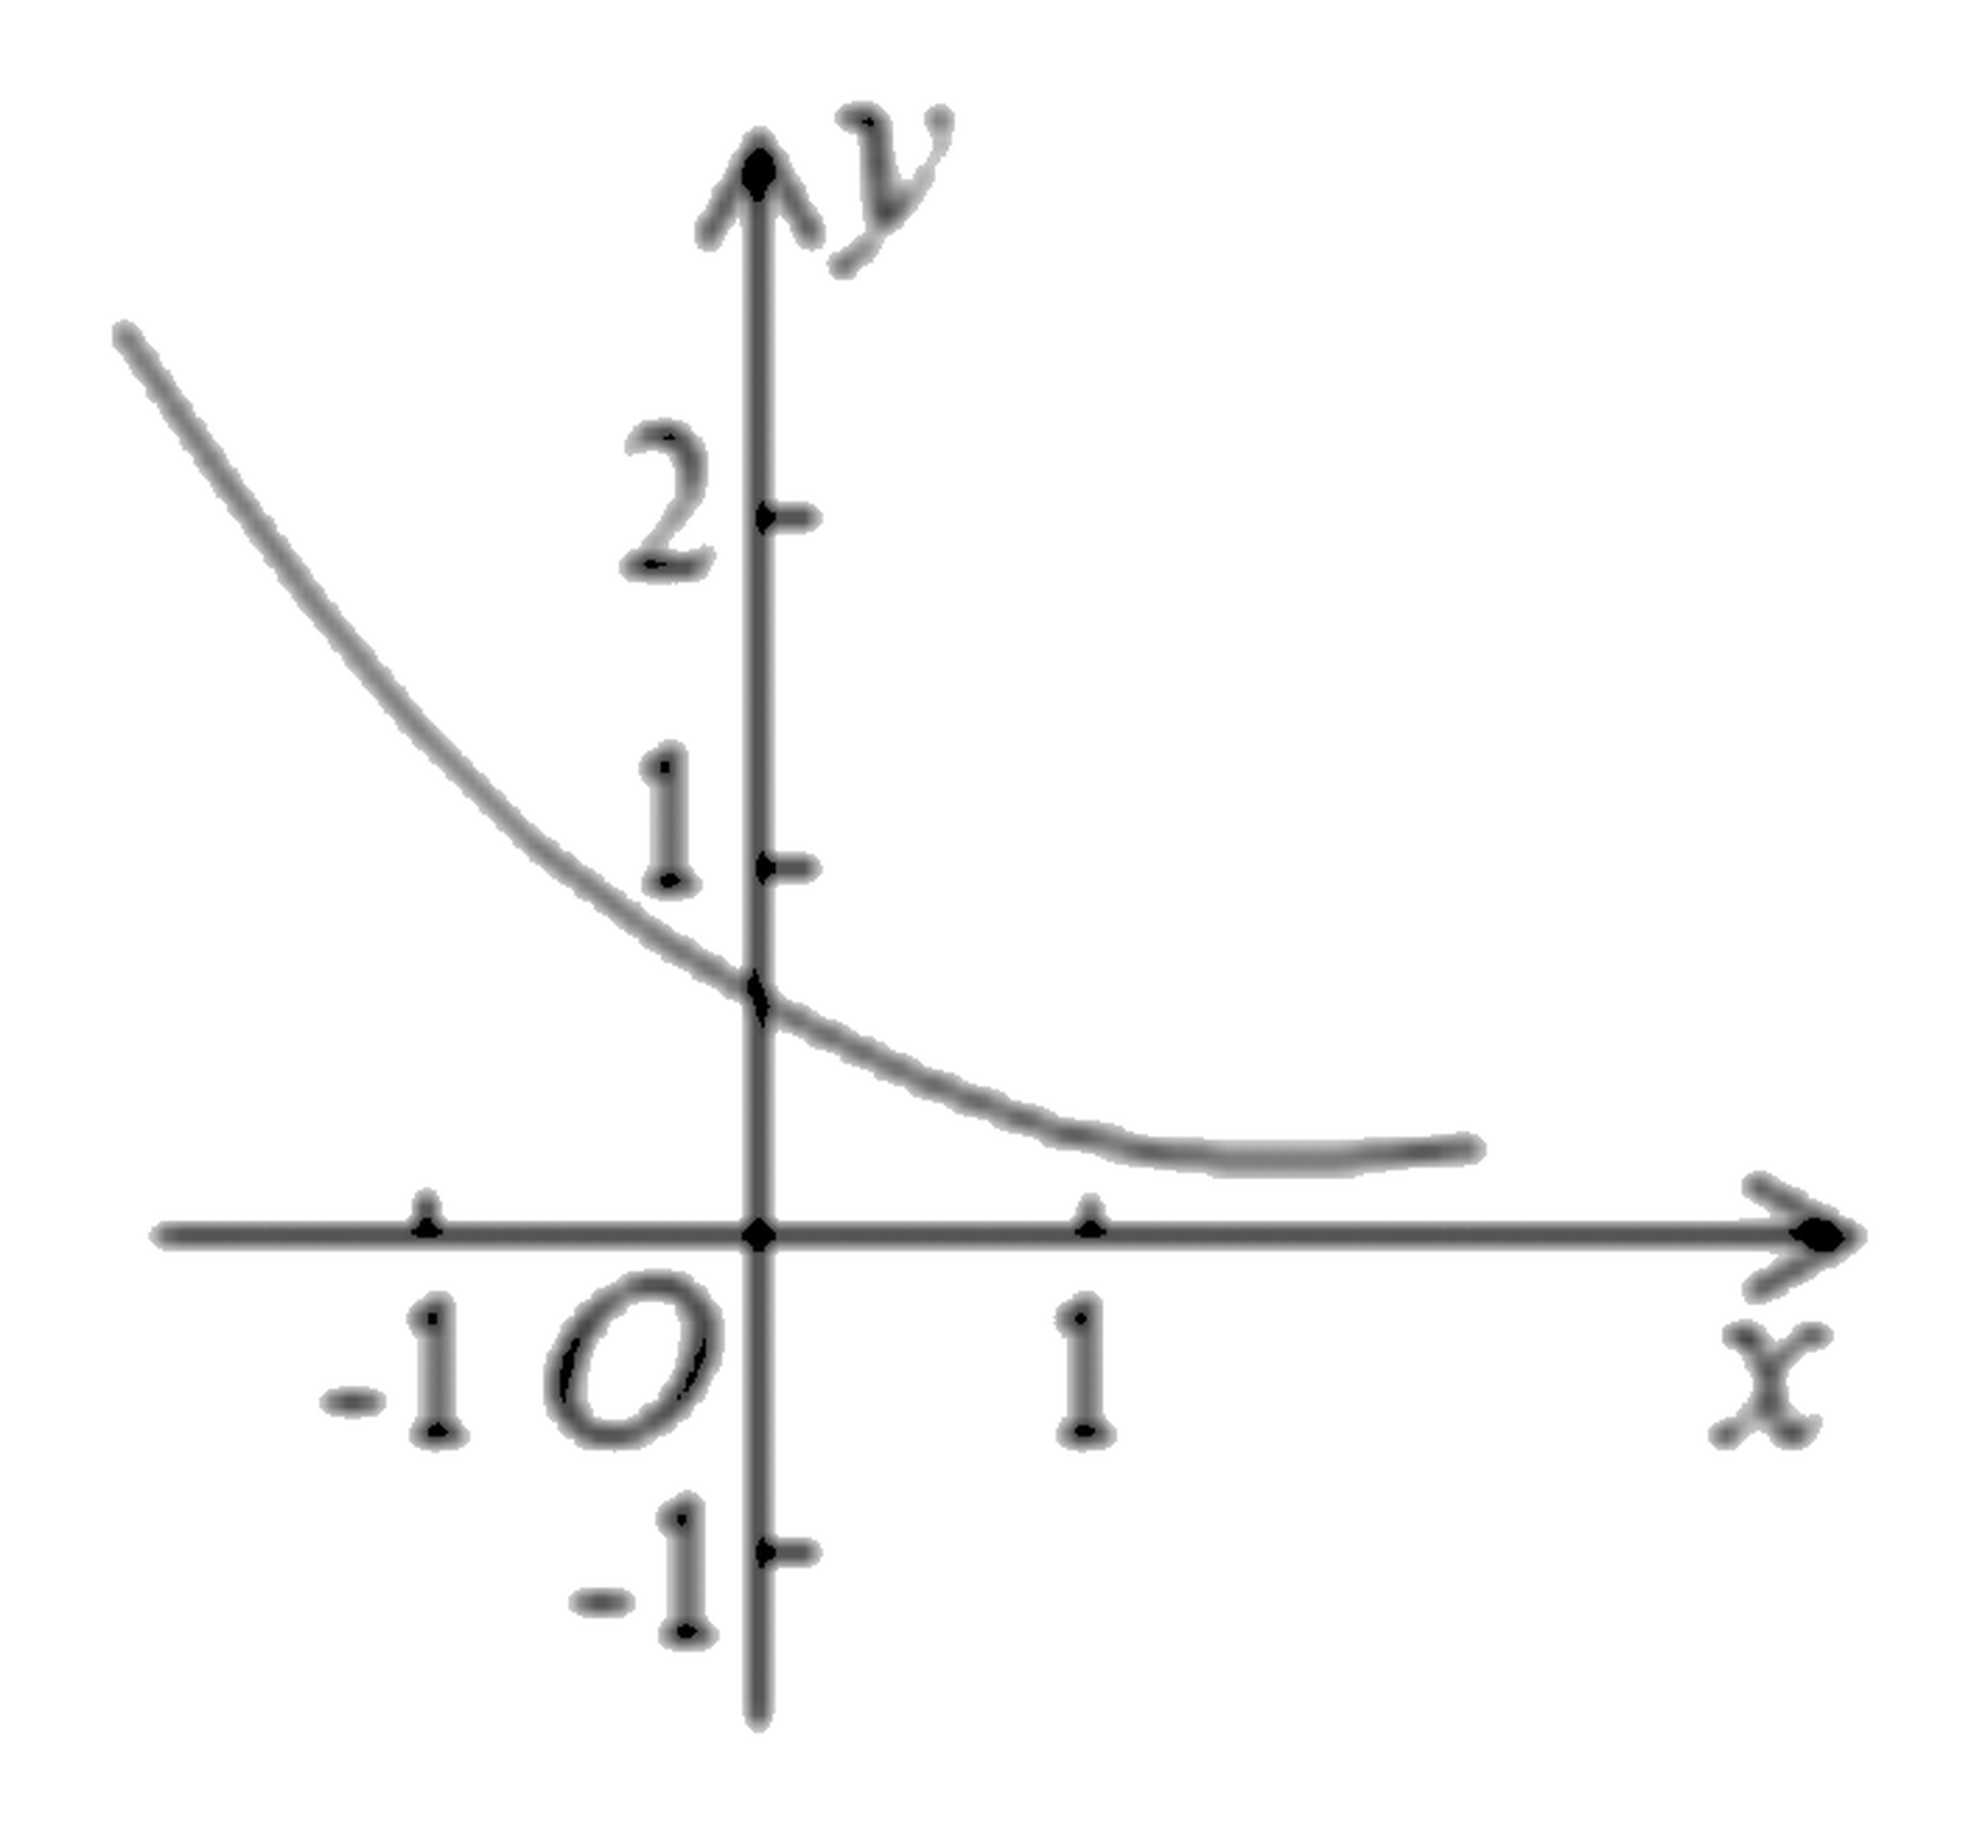
\includegraphics[width=0.30\textwidth]{figures/gao147_q15.png}
\end{center}

\ifanswer
\solbegin
\step{由图象从左到右下降得 $0<a<1$；}
\step{由图象与 $y$ 轴的交点得 $0<a^{-b}<1$，故 $b<0$；}
\step{故 $0<a<1$，$b<0$；故选 $D$.}
\solend
\fi

% === Q16 ===：位数新定义题（无弯引号，放大 04 页 z/q16_stem.png 确认）；四选项横排一行；解析 3 个印刷行
\item 数学运算是指在明晰运算对象的基础上，依据运算法则解决数学问题的素养. 因为运算，数的威力无限；没有运算，数就只是一个符号，对数运算与指数运算是两类重要的运算，对数的运算性质降低了运算的级别，简化了运算，在数学发展史上是伟大的成就. 而位数是指一个自然数有效位的个数，例如：$2^{10}=1024$，所以 $2^{10}$ 的位数为 4. 请你运用所学过的对数运算的知识，估计 $2025^{2026}$ 的位数是\mbox{（\quad）}

\keepwithprev
A. 6697\qquad B. 6698\qquad C. 6699\qquad D. 6700

\ifanswer
\solbegin
\step{设 $2025^{2026}=t$，所以 $\lg t=2026\lg2025$，}
\step{因为 $\lg2025\approx3.3064$，所以 $\lg t\approx6698.8$，}
\step{所以 $t\approx10^{6698.8}\in(10^{6698},10^{6699})$，所以 $2025^{2026}$ 的位数为 6699. 故选 $C$.}
\solend
\fi

\end{enumerate}

\bigsec{三、解答题}

\begin{enumerate}
\setcounter{enumi}{16}

% === Q17 ===：题干＋解析均在 04 页；集合描述竖线 \mid、描述内半角逗号照录；
% 空集 \varnothing、子集 \subseteq（放大 04 页 z/subset_04_q17b.png 确认带下划线）、数集 \R；
% 解析 5 个印刷行，首行末"所以 A=(-∞,-2)∪(3,+∞)"原卷无标点，照录不补
\item 已知集合 $A=\left\{x\mid \dfrac{x+2}{x-3}>0,x\in\R\right\}$，$B=\{x\mid \lvert x-2a\rvert\leqslant2,x\in\R\}$.

(1) 若 $a=1$，求 $A\cap B$；

(2) 若 $A\cap B=\varnothing$，求实数 $a$ 的取值范围.

\ifanswer
\solbegin
\step{由 $\dfrac{x+2}{x-3}>0$，得 $x<-2$ 或 $x>3$，所以 $A=(-\infty,-2)\cup(3,+\infty)$}
\step{(1) 当 $a=1$ 时，$B=\{x\mid \lvert x-2\rvert\leqslant2\}=[0,4]$，于是 $A\cap B=(3,4]$；}
\step{(2) $B=[2a-2,2a+2]$，}
\step{则 $A\cap B=\varnothing\Leftrightarrow[2a-2,2a+2]\subseteq[-2,3]\Leftrightarrow\begin{cases}2a-2\geqslant-2\\2a+2\leqslant3\end{cases}\Leftrightarrow0\leqslant a\leqslant\dfrac{1}{2}$，}
\step{所以实数 $a$ 的取值范围为 $\left[0,\dfrac{1}{2}\right]$.}
\solend
\fi

% === Q18 ===：氟化物／臭氧应用题；"氟化物""（如冰箱等）"全角夹注照录（放大 05 页 z/q18_line1.png 确认）；
% 关系式 $Q=Q_0e^{-0.0025t}$ 原卷独立一行，按一段照录；解析 6 个印刷行
\item 有些家用电器（如冰箱等）使用了氟化物，氟化物的释放破坏了大气上层的臭氧层，使臭氧含量 $Q$ 呈指数函数型变化，在氟化物排放量维持某种水平时，具有关系式

$Q=Q_0e^{-0.0025t}$，其中 $Q_0$ 是臭氧的初始量.

(1) 随时间 $t$ 的增加，臭氧的含量是增加还是减少？

(2) 试估计多少年以后将会有一半的臭氧消失.（用计算器计算）

\ifanswer
\solbegin
\step{(1) 对于函数 $Q=Q_0e^{-0.0025t}$，显然 $Q>0$，}
\step{任取 $t_1$、$t_2\in(0,+\infty)$，且 $t_1<t_2$，则 $t_2-t_1>0$，}
\step{所以 $\dfrac{Q_1}{Q_2}=\dfrac{Q_0e^{-0.0025t_1}}{Q_0e^{-0.0025t_2}}=e^{-0.0025(t_1-t_2)}=e^{0.0025(t_2-t_1)}>e^0=1$，所以 $Q_1>Q_2$，}
\step{故随着时间 $t$ 的增加，臭氧的含量是减少的；}
\step{(2) 令 $\dfrac{Q}{Q_0}=\dfrac{1}{2}$，即 $\dfrac{Q_0e^{-0.0025t}}{Q_0}=e^{-0.0025t}=\dfrac{1}{2}$，得 $-0.0025t=\ln\dfrac{1}{2}\approx-0.6931$，}
\step{解得 $t\approx277$，故估计 277 年以后将会有一半的臭氧消失.}
\solend
\fi

% === Q19 ===：题干用"图像"、解析两处用"图象"逐处照录不统一（05 页）；数集 \Z；
% 题干＋解析前 4 行在 05 页、解析后 3 行在 06 页；解析共 7 个印刷行
\item 已知幂函数 $f(x)=x^{-m^2+4m}(m\in\Z)$ 的图像关于 $y$ 轴对称，且在区间 $(0,+\infty)$ 上是严格增函数.

(1) 求 $m$ 的值；

(2) 求满足不等式 $(2a+1)^m<(a+1)^m$ 的实数 $a$ 的取值范围.

\ifanswer
\solbegin
\step{(1) 由题意得 $-m^2+4m>0$，解得 $0<m<4$，}
\step{因为 $m\in\Z$，所以 $m=1$ 或 $m=2$ 或 $m=3$.}
\step{当 $m=1$ 或 $m=3$ 时，$f(x)=x^3$，图象关于原点对称，不合题意；}
\step{当 $m=2$ 时，$f(x)=x^4$，图象关于 $y$ 轴对称，符合题意，所以 $m=2$.}
\step{(2) 代入 $m=2$，不等式为 $(2a+1)^2<(a+1)^2$，}
\step{得 $(2a+1)^2-(a+1)^2=a(3a+2)<0$，因此 $-\dfrac{2}{3}<a<0$，}
\step{所求范围为 $\left(-\dfrac{2}{3},0\right)$.}
\solend
\fi

% === Q20 ===：指数函数题，题干用"图像"；(3) 长求和式（分数 1/2026、1011/2026、2011/2026、
% 15/2026、1015/2026、2025/2026 放大 06 页 z/q20_sum_06a.png 确认）；题干在 06 页、
% 解析前 6 行在 06 页下半、后 6 行在 07 页上半；解析共 12 个印刷行
\item 已知指数函数 $y=a^x$（$a>0,a\ne1$）的图像经过点 $(1,4)$.

(1) 求实数 $a$ 的值；

(2) 若 $f(x)=(a^x)^2-2\cdot a^x-8$，当 $x\in\R$ 时，不等式 $f(x)>m\cdot4^x-12$ 恒成立，求 $m$ 的取值范围；

(3) 记 $g(x)=\dfrac{1}{a^x+2}$，求证：$g(x)+g(1-x)$ 为定值，并求 $g(0)+g\left(\dfrac{1}{2026}\right)+g\left(\dfrac{1011}{2026}\right)+g\left(\dfrac{2011}{2026}\right)+g\left(\dfrac{1}{2}\right)+g\left(\dfrac{15}{2026}\right)+g\left(\dfrac{1015}{2026}\right)+g\left(\dfrac{2025}{2026}\right)+g(1)$ 的值.

\ifanswer
\solbegin
\step{(1) 将 $(1,4)$ 代入 $y=a^x$，得 $a^1=4$，即 $a=4$.}
\step{(2) 令 $t=4^x$，当 $x\in\R$ 时，$t$ 取遍所有正实数.}
\step{原不等式等价于 $t^2-2t-8>mt-12\Leftrightarrow m<t+\dfrac{4}{t}-2$，}
\step{由基本不等式，$t+\dfrac{4}{t}-2\geqslant2\sqrt{t\cdot\dfrac{4}{t}}-2=2$，}
\step{当且仅当 $t=\dfrac{4}{t}$，即 $t=2$ 时取等号，}
\step{因此原不等式恒成立的充要条件为 $m<2$，即 $m\in(-\infty,2)$.}
\step{(3) 对任意 $x\in\R$，令 $t=4^x>0$，则 $4^{1-x}=\dfrac{4}{t}$，}
\step{从而 $g(x)+g(1-x)=\dfrac{1}{t+2}+\dfrac{1}{\dfrac{4}{t}+2}=\dfrac{1}{t+2}+\dfrac{t}{2(t+2)}=\dfrac{1}{2}$，}
\step{因此 $g(x)+g(1-x)$ 为定值 $\dfrac{1}{2}$.}
\step{原式中，0 与 1、$\dfrac{1}{2026}$ 与 $\dfrac{2025}{2026}$、$\dfrac{1011}{2026}$ 与 $\dfrac{1015}{2026}$、$\dfrac{2011}{2026}$ 与 $\dfrac{15}{2026}$}
\step{分别配对，每对函数值之和均为 $\dfrac{1}{2}$，且 $g\left(\dfrac{1}{2}\right)=\dfrac{1}{4^{\frac12}+2}=\dfrac{1}{4}$，}
\step{所以所求和为 $4\cdot\dfrac{1}{2}+\dfrac{1}{4}=\dfrac{9}{4}$.}
\solend
\fi

% === Q21 ===：不动点新定义题；题干在 07 页、解析续 08／09 页，共 20 个印刷行；
% 判别式两形混用：08 页 (2) cases 内等腰偏高 \Delta、09 页 (3) 扁等边 \triangle，逐处照录不统一
% （放大 /tmp/gao147/z/delta_vs_triangle.png 并排确认）；数集 \R；\forall 照录；
% 第 6—8 行是原卷一个长算式折成的三个印刷行，按印刷行分三条 \step、不并折行
\item 对于二次函数 $y=mx^2+nx+t(m\ne0)$，若存在 $x_0\in\R$，使得 $mx_0^2+nx_0+t=x_0$ 成立，则称 $x_0$ 为二次函数 $y=mx^2+nx+t(m\ne0)$ 的不动点.

(1) 求二次函数 $y=x^2-x-3$ 的不动点；

(2) 若二次函数 $y=2x^2-(3+a)x+a-1$ 有两个不相等的不动点 $x_1$、$x_2$，且 $x_1$、$x_2>0$，求 $\dfrac{x_1}{x_2}+\dfrac{x_2}{x_1}$ 的最小值；

(3) 若对任意实数 $b$，二次函数 $y=ax^2+(b+1)x+(b-1)(a\ne0)$ 恒有不动点，求 $a$ 的取值范围.

\ifanswer
\solbegin
\step{(1) 令 $x^2-x-3=x$，即 $x^2-2x-3=0$，即 $(x-3)(x+1)=0$，}
\step{解得 $x_1=-1$，$x_2=3$，所以不动点为 $-1$ 和 $3$.}
\step{(2) 由题意，$2x^2-(3+a)x+a-1=x$ 有两个不相等的正实数根，}
\step{即方程 $2x^2-(4+a)x+a-1=0$ 有两个不相等的正实数根，}
\step{所以 $\begin{cases}\Delta=(4+a)^2-8(a-1)>0\\x_1+x_2=\dfrac{4+a}{2}>0\\x_1\cdot x_2=\dfrac{a-1}{2}>0\end{cases}$，解得 $a>1$，}% 判别式原卷印等腰偏高粗三角 $\Delta$（放大 08 页 z/delta_08_q21cases.png）
\step{所以 $\dfrac{x_1}{x_2}+\dfrac{x_2}{x_1}=\dfrac{x_1^2+x_2^2}{x_1\cdot x_2}=\dfrac{(x_1+x_2)^2-2x_1\cdot x_2}{x_1\cdot x_2}=\dfrac{(x_1+x_2)^2}{x_1\cdot x_2}-2$}
\step{$=\dfrac{\left(\dfrac{4+a}{2}\right)^2}{\dfrac{a-1}{2}}-2=\dfrac{\dfrac{(a+4)^2}{4}}{\dfrac{a-1}{2}}-2=\dfrac{(a-1+5)^2}{2(a-1)}-2$}
\step{$=\dfrac{(a-1)^2+10(a-1)+25}{2(a-1)}-2=\dfrac{a-1}{2}+\dfrac{25}{2(a-1)}+3$.}
\step{因为 $a>1$，所以 $a-1>0$，}
\step{所以 $\dfrac{a-1}{2}+\dfrac{25}{2(a-1)}+3\geqslant2\sqrt{\dfrac{a-1}{2}\cdot\dfrac{25}{2(a-1)}}+3=8$，}
\step{当且仅当 $\dfrac{a-1}{2}=\dfrac{25}{2(a-1)}$，即 $a=6$ 时等号成立，}
\step{所以 $\dfrac{x_1}{x_2}+\dfrac{x_2}{x_1}$ 的最小值为 $8$.}
\step{(3) 设 $f(x)=ax^2+(b+1)x+b-1$，}
\step{则方程 $f(x)=x$，可化为 $ax^2+(b+1)x+b-1=x$，}
\step{即 $ax^2+bx+b-1=0$，}
\step{由题意得一元二次方程 $ax^2+bx+b-1=0$ 有解，又 $a\ne0$，}
\step{所以方程 $ax^2+bx+b-1=0$ 的判别式 $\triangle=b^2-4a(b-1)\geqslant0$，}% 判别式原卷印扁等边细线三角 $\triangle$（放大 09 页 z/triangle_09_q21.png），与 (2) 高 $\Delta$ 混用、照录不统一
\step{即 $b^2-4ab+4a\geqslant0$，则该不等式对 $\forall b\in\R$ 恒成立，}
\step{则 $(4a)^2-4\times4a\leqslant0$，且 $a\ne0$，解得 $0<a\leqslant1$，}
\step{所以实数 $a$ 的取值范围是 $(0,1]$.}
\solend
\fi

\end{enumerate}

\end{document}
"
% 紧凑版：xelatex "\def\iscompact{1}% 高一147_华师大三附中_期中.tex
%   —— 高一上数学"2026-2027 年华师大三附中高一上期中"（试卷版/答案版/紧凑版）
% 试卷版：xelatex 高一147_华师大三附中_期中.tex
% 答案版：xelatex "\def\isanswer{1}\input{高一147_华师大三附中_期中.tex}"
% 紧凑版：xelatex "\def\iscompact{1}\input{高一147_华师大三附中_期中.tex}"
%
% ① 原始材料：微信公众号"魔都数学加油站"文章，连载"27学年高一147"，原文标题
% "27学年高一147——2026-2027年上海市华师大三附中高一上期中"；
% 原文链接：https://mp.weixin.qq.com/s/X_gPW1JWoTAl2Bky_xEEGw 。
% 正文为 9 张 PNG 页（01/06/08/09 为 2560×3620，02/03/04/05/07 为 4762×6735，
% 同一篇各页分辨率混排，逐页按各自分辨率裁图核对，别按预览比例换算裁框）。
% 体例：混合体例讲评版——19 题中 Q4/Q5/Q7/Q9 只印【答案】、无【解析】，其余 15 题印
% 【解析】（逐题核实，见 ② ②）。题目、答案、解析均据原图转录；卷面粉红色水印
% "魔都数学加油站"及公众号页脚未录入。
% 全卷插图清单（逐页通读 9 页确认）：仅 1 处题目配图——
%   · Q15 递减指数函数小坐标系（03 页右侧：坐标轴、y 轴刻度 2/1/-1、x 轴刻度 -1/1、
%     原点 O、x/y 轴标），为"图像如图所示"的题目配图（选择题选项旁），三版都出；
%     裁自 03 页去粉色水印、去色、4× LANCZOS 放大存 figures/gao147_q15.png；
%   其余 8 页逐页确认无其它题目配图、无【解析】内配图、无表格，
%   亦无"题干写如图而源码漏图"一处；Q12/Q17/Q21 的 cases 块为数学块（非图）。
%
% 卷首标题：原卷印作"2026-2027 年华师大三附中高一上期中"，年份区间按全稿惯例排 en dash；
% 原卷卷面未印副标题，本稿按同期中卷（高一140／141／143／144／145／146）知识模块口径
% 补出"集合与常用逻辑用语、不等式、函数"。
%
% 题号体例（逐页核实定稿）：本卷共 19 题——一、填空题 3—12（10 题）、
% 二、选择题 13—16（4 题）、三、解答题 17—21（5 题）。
% 三节分别 \setcounter{enumi}{2}／{12}／{16}。原卷从第 3 题起、无第 1、2 题，
% 本稿保留原题号；全卷无附加题节（Q21 解析末行"所以实数 a 的取值范围是 (0,1]."
% 为全卷收尾，09 页下半仅水印、无正文）。
%
% ② 与原卷的排版差异：
%   ① 原文从第 3 题起，本稿保留原题号；共 19 题三节；
%   ② 混合体例：原卷 Q4/Q5/Q7/Q9 只印【答案】、无【解析】（分别为 a≤0、(-1,2)、
%      真、(-∞,1)），按 高一140 第 5 题／高一145 Q3 成例提 \ans{}、不补造解析；
%      其余 15 题印【解析】，用 \solbegin…\solend，选择题答案在解析末句"故选 X"
%      （Q13 选 B、Q14 选 B、Q15 选 D、Q16 选 C，逐个放大原图核实）、题干括号
%      \mbox{（\quad）} 留空、不另提 \ans{}；填空／解答答案落在解析里；
%      答案版【答案】/【解析】标记数 = 19（4 个 \ans ＋ 15 个 \solbegin）= 全卷题数；
%   ③ 原卷卷面未印副标题，本稿按知识模块口径补出；
%   ④ 原卷填空横线按全稿惯例排 \blankline[4.4em]；选择题括号排 \mbox{（\quad）}、
%      选项段前按惯例加 \keepwithprev；Q14／Q15 四选项为 2×2 两印刷行（A/B 一行、
%      C/D 一行），用空行分段照录（非一行 \qquad、亦非竖排四行）；解答题不留作答区、
%      不加 \anspace（原卷为讲评版，与 129／131／132／133／136／140／141／143／144／145／146 同）；
%   ⑤ 数集：Q4"A∪B=R"、Q13"f(x)=x^3 在 R 上严格增"、Q17"x∈R"两处、
%      Q20"x∈R"两处、Q21"x_0∈R""∀b∈R"原卷印斜体或黑板粗体 R，按全稿惯例统一改 \R；
%      Q19"m∈Z"改 \Z；本卷未出现 N（\N^* 无对应处）。绝对值排 \lvert…\rvert，
%      集合描述竖线排 \mid；不等号按全稿惯例排 \leqslant／\geqslant（原卷印 \le／\ge 形，
%      【答案】a≤0 亦排 \leqslant）；空集 \varnothing（Q17 两处）；
%      子集 \subseteq（Q17 带下划线，放大 04 页确认）；本卷未出现 \subset／\subsetneq，
%      亦未出现补集上划线 \overline{}；\left…\right 不得拆到不同 $…$ 组；
%   ⑥ 子题标号 (1)(2)(3) 半角括号照录；cases 块整体算一个印刷行（Q3、Q12 一行内
%      两个 cases、Q17、Q21(2)）；本卷解析内无圈数字①②③（无 \text{①} 需求）；
%      数学式内 CJK 用 \text{}（本卷未见）；
%   ⑦ 题干中的中文弯引号按原卷照录：Q7 命题"若 A∪B=B，则 A∩B=A"与
%      (填 " 真 " 或 " 假 ")、Q10 (填 ">" "<" "≤" "或≥")，含引号内空格；
%      注释内一律 ASCII 引号；Q16 位数新定义题逐字放大确认无弯引号
%      （交办提示的"Q16 新定义题"举例未在本卷出现），未补造引号；
%   ⑧ 半角逗号在数学组之间是全稿惯例、非笔误（Q4"$A=(-\infty,0],B=[a,+\infty)$"、
%      Q5"$(a>0,a\ne1)$"、Q17 集合描述内"$>0,x\in R$""$\leqslant2,x\in R$"、
%      Q20 题干"$(a>0,a\ne1)$"、Q21"$y=mx^2+nx+t(m\ne0)$"等），逐处照录别改全角；
%      行末西文句点照录为 ASCII `.`；行中全角逗号／顿号照录；
%      Q7／Q10"(填…)"为半角括号、Q18"（如冰箱等）"为全角括号，逐处照录不统一；
%   ⑨ "图像／图象"逐处照录不统一：题干 5 处用"图像"（Q5"图像恒过定点"、
%      Q9"图像位于直线 y=x 的下方"、Q15"的图像如图所示"、Q19"的图像关于 y 轴对称"、
%      Q20"的图像经过点"），解析 4 处用"图象"（Q15"由图象从左到右下降"
%      "由图象与 y 轴的交点"、Q19"图象关于原点对称""图象关于 y 轴对称"），逐处核、不统一；
%   ⑩ 判别式 Δ/△ 混用是照录项：Q21(2) 解析 cases 块"Δ=(4+a)²−8(a−1)>0"
%      印等腰偏高粗三角 \Delta，Q21(3) 解析"判别式△=b²−4a(b−1)≥0"
%      印扁等边细线三角 \triangle，逐处放大判断、照录不得统一
%      （参照 高一142／144／145 头注④口径，详见 ④）；
%   ⑪ 一条 \step = 原卷解析的一个印刷行，cases 块整体算一个印刷行；别把原卷折行
%      并起来、别把一行拆多条。Q10 七行（跨 01→02 页）、Q12 七行（含一行两 cases）、
%      Q20 十二行（含"原式中…2011/2026 与 15/2026／分别配对…"折行两行）、
%      Q21 二十行（含第 6—8 行一个长算式折成三印刷行、含 cases）均按印刷行逐条断，
%      不丢行；
%   ⑫ 配图：逐页通读 9 页确认全卷仅 Q15 一处题目配图（见 ①），三版都出、
%      \includegraphics[width=0.30\textwidth]；图块较小，未加 \needvspace 大图块守卫
%      （仅 \bigsec 自带 \needvspace{3\baselineskip}）；三版切页审计均"合计异常：无"；
%   ⑬ 跨页续印按题合并：Q3—Q9 在 01 页（Q10 题干在 01 页末、解析首行亦在 01 页末）；
%      Q10 解析续 02 页 6 行、Q11 在 02 页、Q12 题干＋解析前 4 行在 02 页
%      （解析续 03 页 3 行）；"二、选择题"标题与 Q13、Q14、Q15 题干＋解析前 2 行在 03 页
%      （Q15 配图在 03 页右侧）；Q15 解析末行与 Q16、"三、解答题"标题、Q17 在 04 页；
%      Q18 在 05 页、Q19 题干＋解析前 4 行在 05 页（解析续 06 页 3 行）；
%      Q20 题干＋解析前 6 行在 06 页（解析续 07 页 6 行）、Q21 题干＋解析前 3 行在 07 页；
%      Q21 解析续 08 页 13 行、续 09 页 4 行（09 页下半仅水印、无正文）。
%      本稿按题连排，不丢行、不并折行；
%   ⑭ 原卷解析内无红色"法一／法二"之类小标题，故本卷无 \stepm；
%      水印"魔都数学加油站"红色不录入。
%
% ③ 行数复核：一条 \step／\stepm = 原卷解析的一个印刷行，cases 块作一个印刷行计。
%   逐题数（主会话逐页核对定稿）：Q3：1；Q4：0（只印【答案】、提 \ans{}，不计入 \step 账）；
%   Q5：0；Q6：1；Q7：0；Q8：2；Q9：0；Q10：7；Q11：4；Q12：7；Q13：6；Q14：4；
%   Q15：3；Q16：3；Q17：5；Q18：6；Q19：7；Q20：12；Q21：20。
%   合计 88 条 \step（本卷无 \stepm：解析内无红色"法一／法二"类小标题），
%   与原卷逐题印刷行相等。全卷 15 题设 \solbegin…\solend ＋ 4 题一处 \ans{}，
%   答案版【答案】/【解析】标记数 = 19 = 全卷题数。
%
% ④ 判别式／子集符号结论（逐处放大原图照录、不得统一，主会话像素级复核）：
%   判别式全卷 2 处、两形混用逐处照录不统一（参照 高一142／144 头注④口径）：
%     · Q21(2) 解析 cases 块"Δ=(4+a)²−8(a−1)>0" 原卷印等腰偏高粗三角
%       （高>宽、粗笔画），照录 \Delta（放大 08 页 /tmp/gao147/z/delta_08_q21cases.png
%       与 z/delta_vs_triangle.png 左图确认）；
%     · Q21(3) 解析"判别式△=b²−4a(b−1)≥0" 原卷印扁等边细线三角
%       （宽≈高、细线），照录 \triangle（放大 09 页 /tmp/gao147/z/triangle_09_q21.png
%       与 z/delta_vs_triangle.png 右图并排确认）。
%   子集／补集：Q17 解析"[2a−2,2a+2]⊆[−2,3]" 原卷印带下划线 ⊆，照录 \subseteq
%     （放大 04 页 /tmp/gao147/z/subset_04_q17b.png 确认）；Q17"A∩B=∅"空集 \varnothing；
%     集合描述竖线 \mid（Q10 M、Q12 解集、Q17 A/B）；并集 \cup（Q4、Q17）、
%     交集 \cap（Q7、Q17）、不属于 \notin（Q10）；数集 \R／\Z 归一见 ② ⑤。
%   本卷未出现 \subset／\subsetneq，未出现补集上划线 \overline{}。
%
% ⑤ 存疑照录（放大原图确认，照录未改、正文对应处另有 % 注）：
%   1. Q4/Q5/Q7/Q9 只印【答案】、无【解析】，按成例提 \ans{}、不补造解析
%      （混合体例逐题核实，见 ② ②）。
%   2. Q21(2) 判别式高 \Delta 与 Q21(3) 判别式扁 \triangle 两形混用，
%      逐处照录不统一（见 ④）。
%   3. "图像／图象"题干 5 处"图像"、解析 4 处"图象"，逐处照录不统一（见 ② ⑨）。
%   4. Q7／Q10"(填…)"半角括号与 Q18"（如冰箱等）"全角括号，逐处照录不统一。
%   5. Q16 位数新定义题逐字放大确认无弯引号（交办提示的"Q16 新定义题"举例
%      未在本卷出现），未补造引号；全卷弯引号仅 Q7、Q10 两处。
%   6. Q17 解析首行末"所以 A=(-∞,-2)∪(3,+∞)"、Q20(3) 解析"…2011/2026 与 15/2026"
%      行末原卷均无标点，照录未补；Q21(2) 第 6—8 行一个长算式折成三印刷行，
%      按印刷行分三条 \step、不并折行。
%   全卷除此 6 类外未发现其它笔误／自相矛盾处。
%
% ⑥ 跨页续印按题合并说明：见 ② ⑬。
%
\documentclass[a4paper,11pt]{article}
\usepackage{common}

\begin{document}

\examtitlest[3]{2026--2027 年华师大三附中高一上期中}{集合与常用逻辑用语、不等式、函数}

\bigsec{一、填空题}

\begin{enumerate}
\setcounter{enumi}{2}

% === Q3 ===：印【解析】，1 个印刷行（cases 块整体算一行）
\item 函数 $y=(a^2-5a+7)a^x+6-2a$ 是指数函数，则 $a$ 的值为\blankline[4.4em].

\ifanswer
\solbegin
\step{由题意得 $\begin{cases}a^2-5a+7=1\\6-2a=0\end{cases}$，解得 $a=3$.}
\solend
\fi

% === Q4 ===：原卷只印【答案】、无【解析】，按 高一140 第 5 题／高一145 Q3 成例提 \ans{}、不补造解析；
% 题干数学组内半角逗号 $A=(-\infty,0],B=[a,+\infty)$ 照录（放大 01 页 z/q4_stem.png 确认）
\item 已知 $A=(-\infty,0],B=[a,+\infty)$，且 $A\cup B=\R$，则实数 $a$ 的取值范围为\blankline[4.4em].

\ifanswer
\ans{$a\leqslant0$}
\fi

% === Q5 ===：只印【答案】；题干"图像"照录（放大 01 页 z/q5_stem.png 确认）；
% 数学组内半角逗号 $(a>0,a\ne1)$ 照录
\item 函数 $y=a^{x+1}+1(a>0,a\ne1)$ 的图像恒过定点\blankline[4.4em].

\ifanswer
\ans{$(-1,2)$}
\fi

% === Q6 ===：印【解析】，1 个印刷行
\item 已知方程 $x^2+2x-4=0$ 的两个根为 $x_1$、$x_2$，则 $x_1^2+x_2^2$ 的值为\blankline[4.4em].

\ifanswer
\solbegin
\step{$x_1^2+x_2^2=(x_1+x_2)^2-2x_1x_2=4+8=12$.}
\solend
\fi

% === Q7 ===：只印【答案】；中文弯引号"若 A∪B=B，则 A∩B=A"与(填 " 真 " 或 " 假 ")内的空格照录
% （放大 01 页 z/q7_quotes_7x.png、z/q7_tail.png 确认，括号为半角）
\item 命题 “若 $A\cup B=B$，则 $A\cap B=A$” 为\blankline[4.4em]命题(填 “ 真 ” 或 “ 假 ”).

\ifanswer
\ans{真}
\fi

% === Q8 ===：印【解析】，2 个印刷行；不等号按全稿惯例 \geqslant／\leqslant
\item 已知正实数 $a$、$b$ 满足 $a+4b=1$，则 $ab$ 的最大值为\blankline[4.4em].

\ifanswer
\solbegin
\step{$a+4b\geqslant2\sqrt{a\cdot4b}\Rightarrow ab\leqslant\dfrac{1}{16}$，当且仅当 $a=4b=\dfrac{1}{2}$ 时取等号，}
\step{则 $ab$ 的最大值为 $\dfrac{1}{16}$.}
\solend
\fi

% === Q9 ===：只印【答案】；题干"图像"照录（放大 01 页 hi_01_2 确认）
\item 若幂函数 $y=x^s$ 在 $x>1$ 时的图像位于直线 $y=x$ 的下方，则 $s$ 的取值范围是\blankline[4.4em].

\ifanswer
\ans{$(-\infty,1)$}
\fi

% === Q10 ===：印【解析】，共 7 个印刷行（题在 01 页末起 1 行、续 02 页 6 行）；
% 题干跨两印刷行"则 |ab|+1 ____ |a|+|b|（填…）"按一句连排；(填…)为半角括号、引号内空格照录
\item 已知不等式 $\lvert2x+1\rvert+\lvert2x-1\rvert<4$ 的解集为 $M$. 设实数 $a\in M$，$b\notin M$，则 $\lvert ab\rvert+1$\blankline[4.4em] $\lvert a\rvert+\lvert b\rvert$(填 “$>$”，“$<$”，“$\leqslant$” “或$\geqslant$”).

\ifanswer
\solbegin
\step{当 $x<-\dfrac{1}{2}$ 时，不等式化为 $-2x-1+1-2x<4$，即 $x>-1$，所以 $-1<x<-\dfrac{1}{2}$；}
\step{当 $-\dfrac{1}{2}\leqslant x\leqslant\dfrac{1}{2}$ 时，不等式化为 $2x+1-2x+1<4$，即 $2<4$，所以 $-\dfrac{1}{2}\leqslant x\leqslant\dfrac{1}{2}$；}
\step{当 $x>\dfrac{1}{2}$ 时，不等式化为 $2x+1+2x-1<4$，即 $x<1$，所以 $\dfrac{1}{2}<x<1$；}
\step{综上，$M=\{x\mid -1<x<1\}$.}
\step{因为 $a\in M$，$b\notin M$，所以 $\lvert a\rvert<1$，$\lvert b\rvert\geqslant1$.}
\step{而 $\lvert ab\rvert+1-(\lvert a\rvert+\lvert b\rvert)=\lvert ab\rvert+1-\lvert a\rvert-\lvert b\rvert=(\lvert a\rvert-1)(\lvert b\rvert-1)$，}
\step{所以 $\lvert ab\rvert+1\leqslant\lvert a\rvert+\lvert b\rvert$.}
\solend
\fi

% === Q11 ===：印【解析】，4 个印刷行（02 页）
\item 已知 $m>1$，$n>1$，$\lg m=\log_n100$，则 $mn$ 的最小值为\blankline[4.4em].

\ifanswer
\solbegin
\step{由 $m>1$，$n>1$，得 $\lg m>0$，$\lg n>0$，}
\step{因为 $\lg m=\log_n100=\dfrac{\lg100}{\lg n}=\dfrac{2}{\lg n}$，所以 $\lg m\cdot\lg n=2$，}
\step{所以 $\lg(mn)=\lg m+\lg n\geqslant2\sqrt{\lg m\cdot\lg n}=2\sqrt2$，}
\step{当且仅当 $m=n=10^{\sqrt2}$ 时取等号，则 $mn\geqslant10^{2\sqrt2}$，即 $mn$ 的最小值为 $10^{2\sqrt2}$.}
\solend
\fi

% === Q12 ===：印【解析】，共 7 个印刷行（02 页 4 行、03 页 3 行）；
% 第 3 行"则 [cases]，得 [cases]，"两个 cases 块同属一个印刷行，整体作一条 \step（照 高一146 Q11 成例）
\item 已知关于 $x$ 的不等式 $ax^2+bx+c\leqslant1$ 的解集为 $\{x\mid -1\leqslant x\leqslant3\}$. 若关于 $x$ 的不等式 $ax^2+(b-1)x+c-2\leqslant0$ 有且仅有 8 个整数解，则实数 $a$ 的取值范围是\blankline[4.4em].

\ifanswer
\solbegin
\step{由已知关于 $x$ 的不等式 $ax^2+bx+c\leqslant1$ 的解集为 $\{x\mid -1\leqslant x\leqslant3\}$，}
\step{得 $a>0$，且方程 $ax^2+bx+c-1=0$ 的两根分别为 $-1$ 和 $3$，}
\step{则 $\begin{cases}-1+3=-\dfrac{b}{a}\\-1\times3=\dfrac{c-1}{a}\end{cases}$，得 $\begin{cases}b=-2a\\c=1-3a\end{cases}$，}
\step{不等式 $ax^2+(b-1)x+c-2\leqslant0$ 等价于 $ax^2-(2a+1)x-(3a+1)\leqslant0$，}
\step{即 $\left[x-\left(3+\dfrac{1}{a}\right)\right](x+1)\leqslant0$，解得 $-1\leqslant x\leqslant3+\dfrac{1}{a}$，}
\step{因为关于 $x$ 的不等式 $ax^2+(b-1)x+c-2\leqslant0$ 有且仅有 8 个整数解，}
\step{因此 $6\leqslant3+\dfrac{1}{a}<7$，即 $3\leqslant\dfrac{1}{a}<4$，解得 $\dfrac{1}{4}<a\leqslant\dfrac{1}{3}$，所以 $a$ 的取值范围为 $\left(\dfrac{1}{4},\dfrac{1}{3}\right]$.}
\solend
\fi

\end{enumerate}

\bigsec{二、选择题}

\begin{enumerate}
\setcounter{enumi}{12}

% === Q13 ===：题干＋选项＋解析均在 03 页；四选项横排一行；解析 6 个印刷行，末句"故选 B."
\item $a<b<0$，则下列不等式能成立的是\mbox{（\quad）}

\keepwithprev
A. $\dfrac{a}{b}<1$\qquad B. $\lvert a\rvert>-b$\qquad C. $\dfrac{1}{a}<\dfrac{1}{b}$\qquad D. $b^3<a^3$

\ifanswer
\solbegin
\step{对于 $A$，令 $a=-4$，$b=-3$，满足 $a<b<0$，但 $\dfrac{a}{b}>1$，故 $A$ 错误，}
\step{对于 $B$，因为 $a<b<0$，所以 $-a>-b>0$，即 $\lvert a\rvert>-b$，故 $B$ 正确，}
\step{对于 $C$，令 $a=-4$，$b=-3$，满足 $a<b<0$，但 $\dfrac{1}{a}>\dfrac{1}{b}$，故 $C$ 错误，}
\step{对于 $D$，$f(x)=x^3$ 在 $\R$ 上严格增，因为 $a<b$，所以 $f(a)<f(b)$，}
\step{即 $a^3<b^3$，故 $D$ 错误.}
\step{故选 $B$.}
\solend
\fi

% === Q14 ===：四选项原卷为 2×2 两印刷行（A/B 一行、C/D 一行），用空行分段照录；解析 4 个印刷行
\item 已知 $a$、$b$ 为实数，若 $\alpha:ab=0$，$\beta:a^2+\sqrt{b}=0$，则 $\alpha$ 是 $\beta$ 的\mbox{（\quad）}

\keepwithprev
A. 充分不必要条件\qquad\qquad B. 必要不充分条件

C. 充要条件\qquad\qquad D. 既不充分也不必要条件

\ifanswer
\solbegin
\step{$\beta:a^2+\sqrt{b}=0$，所以 $a=0$ 且 $b=0$，}
\step{由 $a=0$，$b=0\Rightarrow ab=0$，反之不成立.}
\step{所以 $ab=0$ 是 $a=0$，$b=0$ 的必要不充分条件，即 $\alpha$ 是 $\beta$ 的必要不充分条件，}
\step{故选 $B$.}
\solend
\fi

% === Q15 ===：题目配图（03 页右侧小坐标系），三版都出；题干用"图像"、解析用"图象"逐处照录；
% 四选项 2×2 两印刷行；解析 3 个印刷行（03 页 2 行、04 页 1 行，末句"故选 D."与前行同一印刷行）
\item 函数 $f(x)=a^{x-b}$ 的图像如图所示，其中 $a$、$b$ 为常数，则下列结论正确的是\mbox{（\quad）}

\keepwithprev
A. $a>1$，$b<0$\qquad\qquad B. $a>1$，$b>0$

C. $0<a<1$，$b>0$\qquad\qquad D. $0<a<1$，$b<0$

\begin{center}
% 递减指数函数小坐标系图取 03 页右侧，去粉色水印、去色、4× LANCZOS 放大；题目配图三版都出
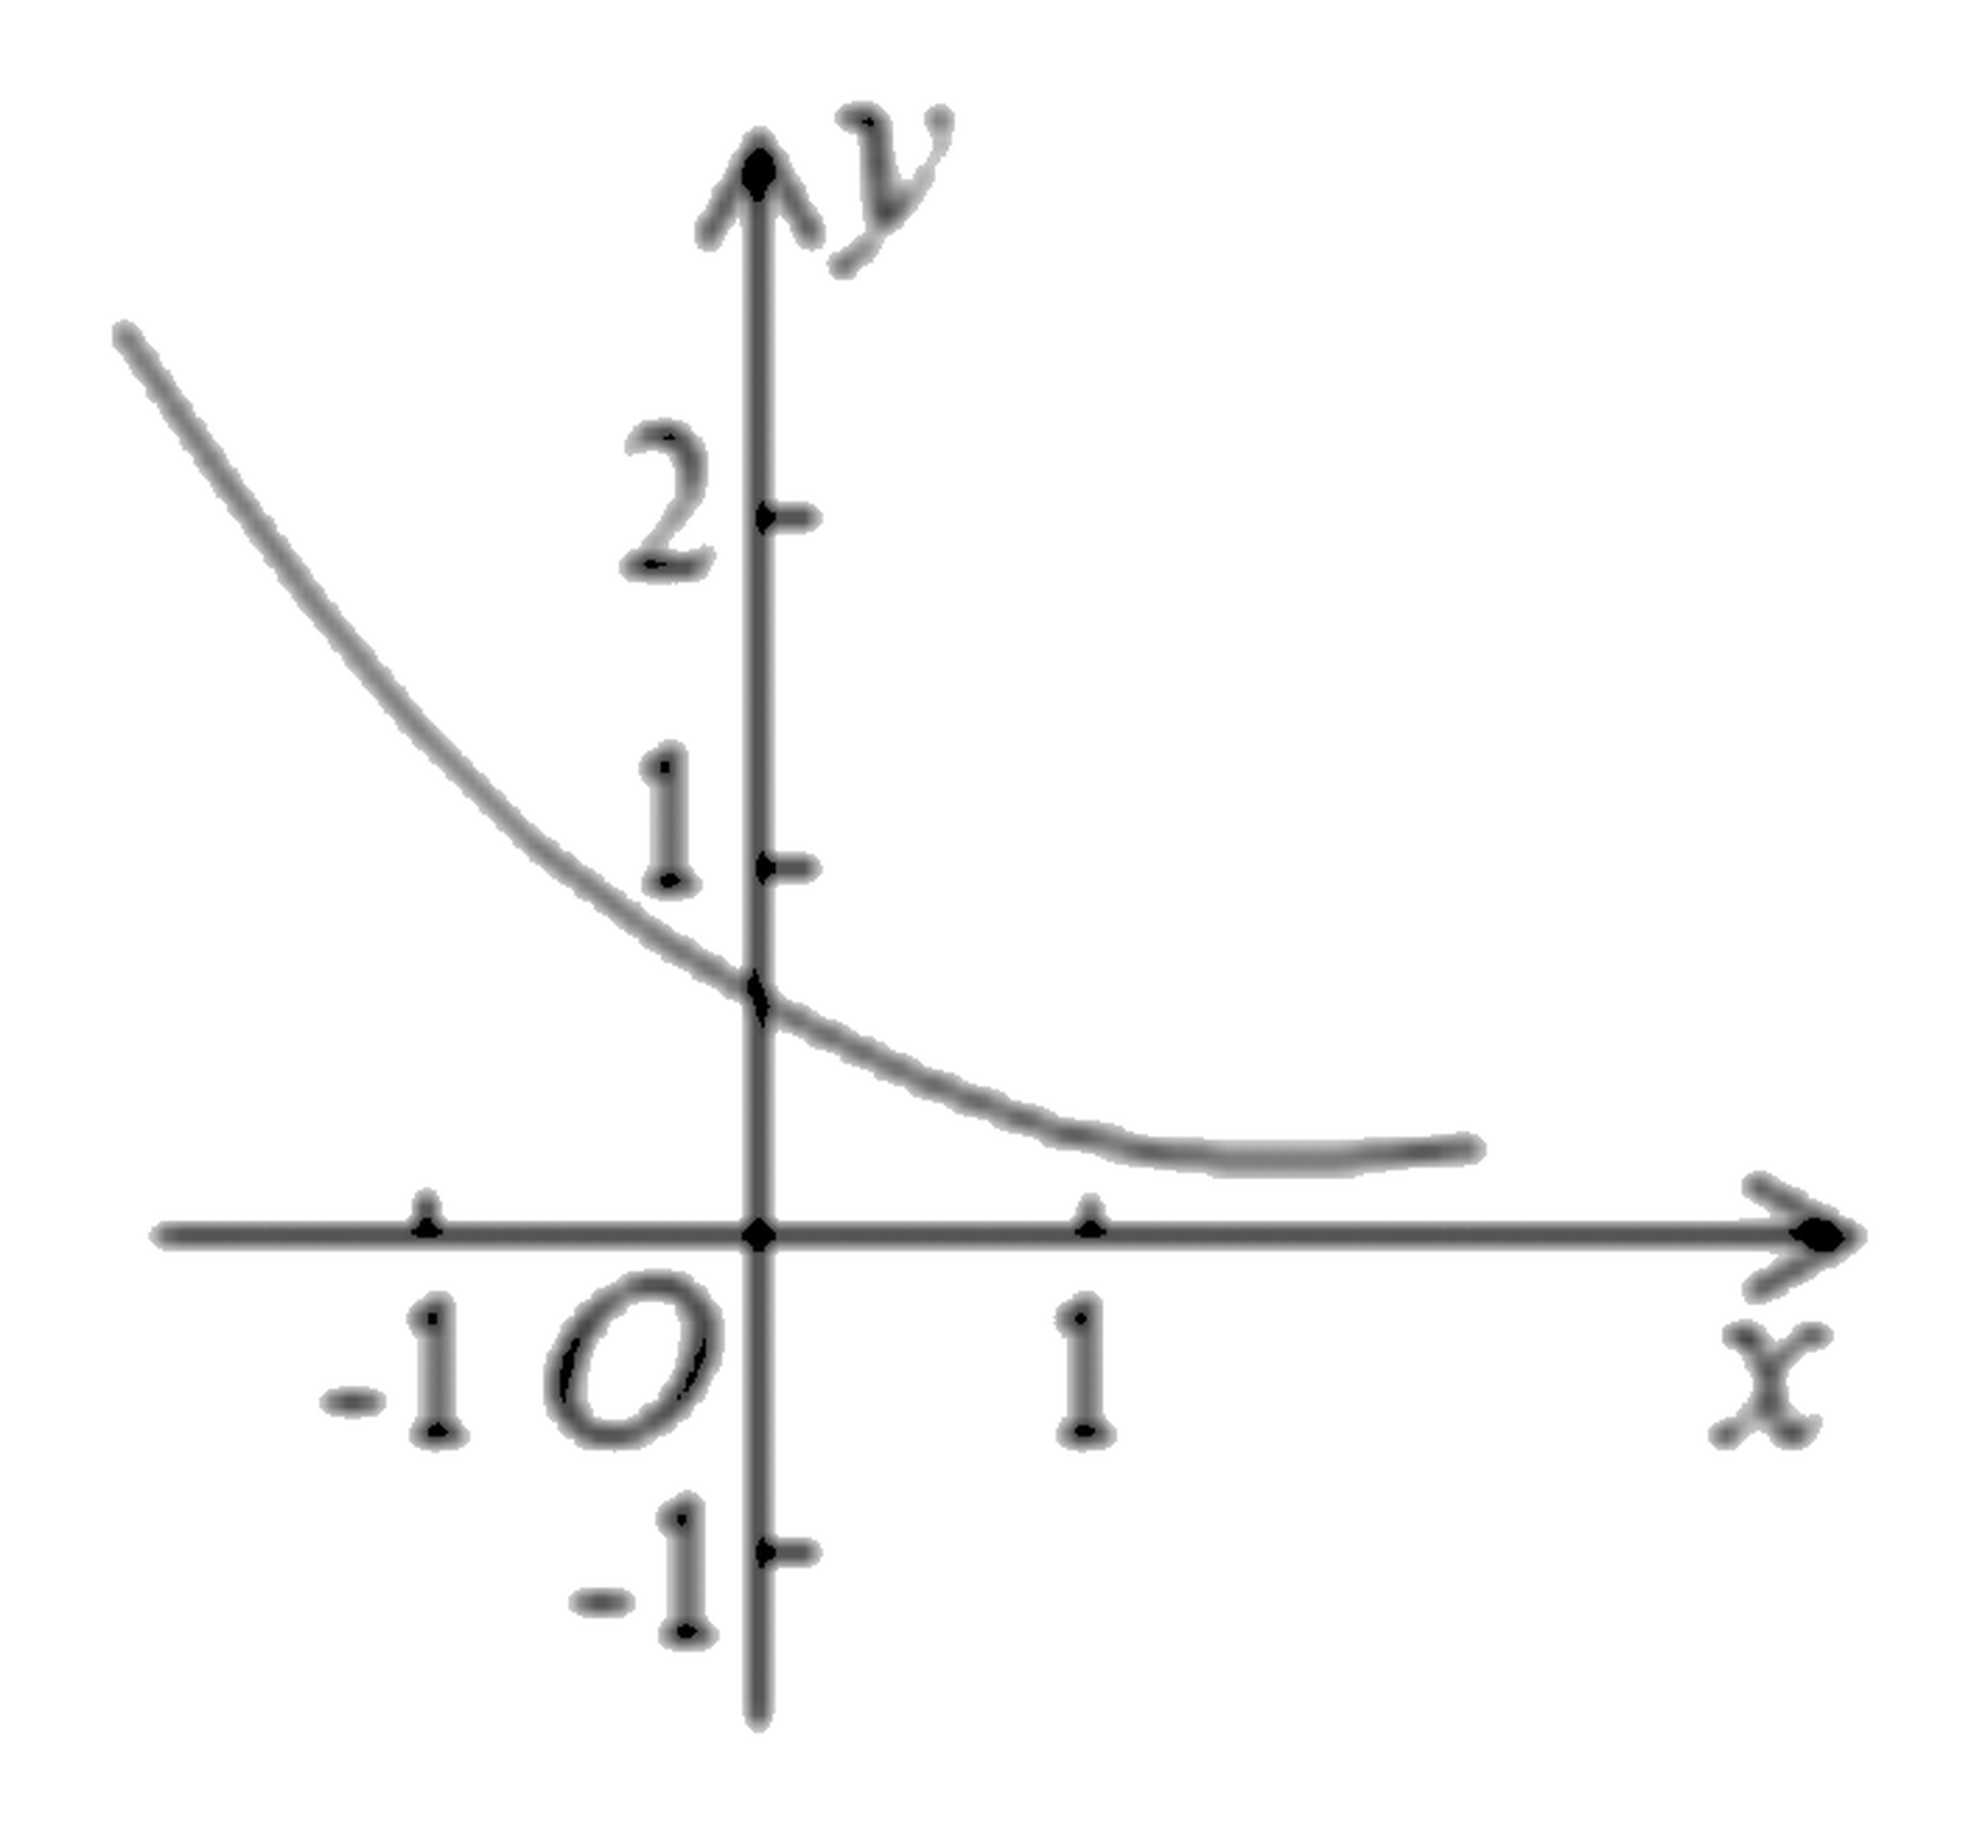
\includegraphics[width=0.30\textwidth]{figures/gao147_q15.png}
\end{center}

\ifanswer
\solbegin
\step{由图象从左到右下降得 $0<a<1$；}
\step{由图象与 $y$ 轴的交点得 $0<a^{-b}<1$，故 $b<0$；}
\step{故 $0<a<1$，$b<0$；故选 $D$.}
\solend
\fi

% === Q16 ===：位数新定义题（无弯引号，放大 04 页 z/q16_stem.png 确认）；四选项横排一行；解析 3 个印刷行
\item 数学运算是指在明晰运算对象的基础上，依据运算法则解决数学问题的素养. 因为运算，数的威力无限；没有运算，数就只是一个符号，对数运算与指数运算是两类重要的运算，对数的运算性质降低了运算的级别，简化了运算，在数学发展史上是伟大的成就. 而位数是指一个自然数有效位的个数，例如：$2^{10}=1024$，所以 $2^{10}$ 的位数为 4. 请你运用所学过的对数运算的知识，估计 $2025^{2026}$ 的位数是\mbox{（\quad）}

\keepwithprev
A. 6697\qquad B. 6698\qquad C. 6699\qquad D. 6700

\ifanswer
\solbegin
\step{设 $2025^{2026}=t$，所以 $\lg t=2026\lg2025$，}
\step{因为 $\lg2025\approx3.3064$，所以 $\lg t\approx6698.8$，}
\step{所以 $t\approx10^{6698.8}\in(10^{6698},10^{6699})$，所以 $2025^{2026}$ 的位数为 6699. 故选 $C$.}
\solend
\fi

\end{enumerate}

\bigsec{三、解答题}

\begin{enumerate}
\setcounter{enumi}{16}

% === Q17 ===：题干＋解析均在 04 页；集合描述竖线 \mid、描述内半角逗号照录；
% 空集 \varnothing、子集 \subseteq（放大 04 页 z/subset_04_q17b.png 确认带下划线）、数集 \R；
% 解析 5 个印刷行，首行末"所以 A=(-∞,-2)∪(3,+∞)"原卷无标点，照录不补
\item 已知集合 $A=\left\{x\mid \dfrac{x+2}{x-3}>0,x\in\R\right\}$，$B=\{x\mid \lvert x-2a\rvert\leqslant2,x\in\R\}$.

(1) 若 $a=1$，求 $A\cap B$；

(2) 若 $A\cap B=\varnothing$，求实数 $a$ 的取值范围.

\ifanswer
\solbegin
\step{由 $\dfrac{x+2}{x-3}>0$，得 $x<-2$ 或 $x>3$，所以 $A=(-\infty,-2)\cup(3,+\infty)$}
\step{(1) 当 $a=1$ 时，$B=\{x\mid \lvert x-2\rvert\leqslant2\}=[0,4]$，于是 $A\cap B=(3,4]$；}
\step{(2) $B=[2a-2,2a+2]$，}
\step{则 $A\cap B=\varnothing\Leftrightarrow[2a-2,2a+2]\subseteq[-2,3]\Leftrightarrow\begin{cases}2a-2\geqslant-2\\2a+2\leqslant3\end{cases}\Leftrightarrow0\leqslant a\leqslant\dfrac{1}{2}$，}
\step{所以实数 $a$ 的取值范围为 $\left[0,\dfrac{1}{2}\right]$.}
\solend
\fi

% === Q18 ===：氟化物／臭氧应用题；"氟化物""（如冰箱等）"全角夹注照录（放大 05 页 z/q18_line1.png 确认）；
% 关系式 $Q=Q_0e^{-0.0025t}$ 原卷独立一行，按一段照录；解析 6 个印刷行
\item 有些家用电器（如冰箱等）使用了氟化物，氟化物的释放破坏了大气上层的臭氧层，使臭氧含量 $Q$ 呈指数函数型变化，在氟化物排放量维持某种水平时，具有关系式

$Q=Q_0e^{-0.0025t}$，其中 $Q_0$ 是臭氧的初始量.

(1) 随时间 $t$ 的增加，臭氧的含量是增加还是减少？

(2) 试估计多少年以后将会有一半的臭氧消失.（用计算器计算）

\ifanswer
\solbegin
\step{(1) 对于函数 $Q=Q_0e^{-0.0025t}$，显然 $Q>0$，}
\step{任取 $t_1$、$t_2\in(0,+\infty)$，且 $t_1<t_2$，则 $t_2-t_1>0$，}
\step{所以 $\dfrac{Q_1}{Q_2}=\dfrac{Q_0e^{-0.0025t_1}}{Q_0e^{-0.0025t_2}}=e^{-0.0025(t_1-t_2)}=e^{0.0025(t_2-t_1)}>e^0=1$，所以 $Q_1>Q_2$，}
\step{故随着时间 $t$ 的增加，臭氧的含量是减少的；}
\step{(2) 令 $\dfrac{Q}{Q_0}=\dfrac{1}{2}$，即 $\dfrac{Q_0e^{-0.0025t}}{Q_0}=e^{-0.0025t}=\dfrac{1}{2}$，得 $-0.0025t=\ln\dfrac{1}{2}\approx-0.6931$，}
\step{解得 $t\approx277$，故估计 277 年以后将会有一半的臭氧消失.}
\solend
\fi

% === Q19 ===：题干用"图像"、解析两处用"图象"逐处照录不统一（05 页）；数集 \Z；
% 题干＋解析前 4 行在 05 页、解析后 3 行在 06 页；解析共 7 个印刷行
\item 已知幂函数 $f(x)=x^{-m^2+4m}(m\in\Z)$ 的图像关于 $y$ 轴对称，且在区间 $(0,+\infty)$ 上是严格增函数.

(1) 求 $m$ 的值；

(2) 求满足不等式 $(2a+1)^m<(a+1)^m$ 的实数 $a$ 的取值范围.

\ifanswer
\solbegin
\step{(1) 由题意得 $-m^2+4m>0$，解得 $0<m<4$，}
\step{因为 $m\in\Z$，所以 $m=1$ 或 $m=2$ 或 $m=3$.}
\step{当 $m=1$ 或 $m=3$ 时，$f(x)=x^3$，图象关于原点对称，不合题意；}
\step{当 $m=2$ 时，$f(x)=x^4$，图象关于 $y$ 轴对称，符合题意，所以 $m=2$.}
\step{(2) 代入 $m=2$，不等式为 $(2a+1)^2<(a+1)^2$，}
\step{得 $(2a+1)^2-(a+1)^2=a(3a+2)<0$，因此 $-\dfrac{2}{3}<a<0$，}
\step{所求范围为 $\left(-\dfrac{2}{3},0\right)$.}
\solend
\fi

% === Q20 ===：指数函数题，题干用"图像"；(3) 长求和式（分数 1/2026、1011/2026、2011/2026、
% 15/2026、1015/2026、2025/2026 放大 06 页 z/q20_sum_06a.png 确认）；题干在 06 页、
% 解析前 6 行在 06 页下半、后 6 行在 07 页上半；解析共 12 个印刷行
\item 已知指数函数 $y=a^x$（$a>0,a\ne1$）的图像经过点 $(1,4)$.

(1) 求实数 $a$ 的值；

(2) 若 $f(x)=(a^x)^2-2\cdot a^x-8$，当 $x\in\R$ 时，不等式 $f(x)>m\cdot4^x-12$ 恒成立，求 $m$ 的取值范围；

(3) 记 $g(x)=\dfrac{1}{a^x+2}$，求证：$g(x)+g(1-x)$ 为定值，并求 $g(0)+g\left(\dfrac{1}{2026}\right)+g\left(\dfrac{1011}{2026}\right)+g\left(\dfrac{2011}{2026}\right)+g\left(\dfrac{1}{2}\right)+g\left(\dfrac{15}{2026}\right)+g\left(\dfrac{1015}{2026}\right)+g\left(\dfrac{2025}{2026}\right)+g(1)$ 的值.

\ifanswer
\solbegin
\step{(1) 将 $(1,4)$ 代入 $y=a^x$，得 $a^1=4$，即 $a=4$.}
\step{(2) 令 $t=4^x$，当 $x\in\R$ 时，$t$ 取遍所有正实数.}
\step{原不等式等价于 $t^2-2t-8>mt-12\Leftrightarrow m<t+\dfrac{4}{t}-2$，}
\step{由基本不等式，$t+\dfrac{4}{t}-2\geqslant2\sqrt{t\cdot\dfrac{4}{t}}-2=2$，}
\step{当且仅当 $t=\dfrac{4}{t}$，即 $t=2$ 时取等号，}
\step{因此原不等式恒成立的充要条件为 $m<2$，即 $m\in(-\infty,2)$.}
\step{(3) 对任意 $x\in\R$，令 $t=4^x>0$，则 $4^{1-x}=\dfrac{4}{t}$，}
\step{从而 $g(x)+g(1-x)=\dfrac{1}{t+2}+\dfrac{1}{\dfrac{4}{t}+2}=\dfrac{1}{t+2}+\dfrac{t}{2(t+2)}=\dfrac{1}{2}$，}
\step{因此 $g(x)+g(1-x)$ 为定值 $\dfrac{1}{2}$.}
\step{原式中，0 与 1、$\dfrac{1}{2026}$ 与 $\dfrac{2025}{2026}$、$\dfrac{1011}{2026}$ 与 $\dfrac{1015}{2026}$、$\dfrac{2011}{2026}$ 与 $\dfrac{15}{2026}$}
\step{分别配对，每对函数值之和均为 $\dfrac{1}{2}$，且 $g\left(\dfrac{1}{2}\right)=\dfrac{1}{4^{\frac12}+2}=\dfrac{1}{4}$，}
\step{所以所求和为 $4\cdot\dfrac{1}{2}+\dfrac{1}{4}=\dfrac{9}{4}$.}
\solend
\fi

% === Q21 ===：不动点新定义题；题干在 07 页、解析续 08／09 页，共 20 个印刷行；
% 判别式两形混用：08 页 (2) cases 内等腰偏高 \Delta、09 页 (3) 扁等边 \triangle，逐处照录不统一
% （放大 /tmp/gao147/z/delta_vs_triangle.png 并排确认）；数集 \R；\forall 照录；
% 第 6—8 行是原卷一个长算式折成的三个印刷行，按印刷行分三条 \step、不并折行
\item 对于二次函数 $y=mx^2+nx+t(m\ne0)$，若存在 $x_0\in\R$，使得 $mx_0^2+nx_0+t=x_0$ 成立，则称 $x_0$ 为二次函数 $y=mx^2+nx+t(m\ne0)$ 的不动点.

(1) 求二次函数 $y=x^2-x-3$ 的不动点；

(2) 若二次函数 $y=2x^2-(3+a)x+a-1$ 有两个不相等的不动点 $x_1$、$x_2$，且 $x_1$、$x_2>0$，求 $\dfrac{x_1}{x_2}+\dfrac{x_2}{x_1}$ 的最小值；

(3) 若对任意实数 $b$，二次函数 $y=ax^2+(b+1)x+(b-1)(a\ne0)$ 恒有不动点，求 $a$ 的取值范围.

\ifanswer
\solbegin
\step{(1) 令 $x^2-x-3=x$，即 $x^2-2x-3=0$，即 $(x-3)(x+1)=0$，}
\step{解得 $x_1=-1$，$x_2=3$，所以不动点为 $-1$ 和 $3$.}
\step{(2) 由题意，$2x^2-(3+a)x+a-1=x$ 有两个不相等的正实数根，}
\step{即方程 $2x^2-(4+a)x+a-1=0$ 有两个不相等的正实数根，}
\step{所以 $\begin{cases}\Delta=(4+a)^2-8(a-1)>0\\x_1+x_2=\dfrac{4+a}{2}>0\\x_1\cdot x_2=\dfrac{a-1}{2}>0\end{cases}$，解得 $a>1$，}% 判别式原卷印等腰偏高粗三角 $\Delta$（放大 08 页 z/delta_08_q21cases.png）
\step{所以 $\dfrac{x_1}{x_2}+\dfrac{x_2}{x_1}=\dfrac{x_1^2+x_2^2}{x_1\cdot x_2}=\dfrac{(x_1+x_2)^2-2x_1\cdot x_2}{x_1\cdot x_2}=\dfrac{(x_1+x_2)^2}{x_1\cdot x_2}-2$}
\step{$=\dfrac{\left(\dfrac{4+a}{2}\right)^2}{\dfrac{a-1}{2}}-2=\dfrac{\dfrac{(a+4)^2}{4}}{\dfrac{a-1}{2}}-2=\dfrac{(a-1+5)^2}{2(a-1)}-2$}
\step{$=\dfrac{(a-1)^2+10(a-1)+25}{2(a-1)}-2=\dfrac{a-1}{2}+\dfrac{25}{2(a-1)}+3$.}
\step{因为 $a>1$，所以 $a-1>0$，}
\step{所以 $\dfrac{a-1}{2}+\dfrac{25}{2(a-1)}+3\geqslant2\sqrt{\dfrac{a-1}{2}\cdot\dfrac{25}{2(a-1)}}+3=8$，}
\step{当且仅当 $\dfrac{a-1}{2}=\dfrac{25}{2(a-1)}$，即 $a=6$ 时等号成立，}
\step{所以 $\dfrac{x_1}{x_2}+\dfrac{x_2}{x_1}$ 的最小值为 $8$.}
\step{(3) 设 $f(x)=ax^2+(b+1)x+b-1$，}
\step{则方程 $f(x)=x$，可化为 $ax^2+(b+1)x+b-1=x$，}
\step{即 $ax^2+bx+b-1=0$，}
\step{由题意得一元二次方程 $ax^2+bx+b-1=0$ 有解，又 $a\ne0$，}
\step{所以方程 $ax^2+bx+b-1=0$ 的判别式 $\triangle=b^2-4a(b-1)\geqslant0$，}% 判别式原卷印扁等边细线三角 $\triangle$（放大 09 页 z/triangle_09_q21.png），与 (2) 高 $\Delta$ 混用、照录不统一
\step{即 $b^2-4ab+4a\geqslant0$，则该不等式对 $\forall b\in\R$ 恒成立，}
\step{则 $(4a)^2-4\times4a\leqslant0$，且 $a\ne0$，解得 $0<a\leqslant1$，}
\step{所以实数 $a$ 的取值范围是 $(0,1]$.}
\solend
\fi

\end{enumerate}

\end{document}
"
%
% ① 原始材料：微信公众号"魔都数学加油站"文章，连载"27学年高一147"，原文标题
% "27学年高一147——2026-2027年上海市华师大三附中高一上期中"；
% 原文链接：https://mp.weixin.qq.com/s/X_gPW1JWoTAl2Bky_xEEGw 。
% 正文为 9 张 PNG 页（01/06/08/09 为 2560×3620，02/03/04/05/07 为 4762×6735，
% 同一篇各页分辨率混排，逐页按各自分辨率裁图核对，别按预览比例换算裁框）。
% 体例：混合体例讲评版——19 题中 Q4/Q5/Q7/Q9 只印【答案】、无【解析】，其余 15 题印
% 【解析】（逐题核实，见 ② ②）。题目、答案、解析均据原图转录；卷面粉红色水印
% "魔都数学加油站"及公众号页脚未录入。
% 全卷插图清单（逐页通读 9 页确认）：仅 1 处题目配图——
%   · Q15 递减指数函数小坐标系（03 页右侧：坐标轴、y 轴刻度 2/1/-1、x 轴刻度 -1/1、
%     原点 O、x/y 轴标），为"图像如图所示"的题目配图（选择题选项旁），三版都出；
%     裁自 03 页去粉色水印、去色、4× LANCZOS 放大存 figures/gao147_q15.png；
%   其余 8 页逐页确认无其它题目配图、无【解析】内配图、无表格，
%   亦无"题干写如图而源码漏图"一处；Q12/Q17/Q21 的 cases 块为数学块（非图）。
%
% 卷首标题：原卷印作"2026-2027 年华师大三附中高一上期中"，年份区间按全稿惯例排 en dash；
% 原卷卷面未印副标题，本稿按同期中卷（高一140／141／143／144／145／146）知识模块口径
% 补出"集合与常用逻辑用语、不等式、函数"。
%
% 题号体例（逐页核实定稿）：本卷共 19 题——一、填空题 3—12（10 题）、
% 二、选择题 13—16（4 题）、三、解答题 17—21（5 题）。
% 三节分别 \setcounter{enumi}{2}／{12}／{16}。原卷从第 3 题起、无第 1、2 题，
% 本稿保留原题号；全卷无附加题节（Q21 解析末行"所以实数 a 的取值范围是 (0,1]."
% 为全卷收尾，09 页下半仅水印、无正文）。
%
% ② 与原卷的排版差异：
%   ① 原文从第 3 题起，本稿保留原题号；共 19 题三节；
%   ② 混合体例：原卷 Q4/Q5/Q7/Q9 只印【答案】、无【解析】（分别为 a≤0、(-1,2)、
%      真、(-∞,1)），按 高一140 第 5 题／高一145 Q3 成例提 \ans{}、不补造解析；
%      其余 15 题印【解析】，用 \solbegin…\solend，选择题答案在解析末句"故选 X"
%      （Q13 选 B、Q14 选 B、Q15 选 D、Q16 选 C，逐个放大原图核实）、题干括号
%      \mbox{（\quad）} 留空、不另提 \ans{}；填空／解答答案落在解析里；
%      答案版【答案】/【解析】标记数 = 19（4 个 \ans ＋ 15 个 \solbegin）= 全卷题数；
%   ③ 原卷卷面未印副标题，本稿按知识模块口径补出；
%   ④ 原卷填空横线按全稿惯例排 \blankline[4.4em]；选择题括号排 \mbox{（\quad）}、
%      选项段前按惯例加 \keepwithprev；Q14／Q15 四选项为 2×2 两印刷行（A/B 一行、
%      C/D 一行），用空行分段照录（非一行 \qquad、亦非竖排四行）；解答题不留作答区、
%      不加 \anspace（原卷为讲评版，与 129／131／132／133／136／140／141／143／144／145／146 同）；
%   ⑤ 数集：Q4"A∪B=R"、Q13"f(x)=x^3 在 R 上严格增"、Q17"x∈R"两处、
%      Q20"x∈R"两处、Q21"x_0∈R""∀b∈R"原卷印斜体或黑板粗体 R，按全稿惯例统一改 \R；
%      Q19"m∈Z"改 \Z；本卷未出现 N（\N^* 无对应处）。绝对值排 \lvert…\rvert，
%      集合描述竖线排 \mid；不等号按全稿惯例排 \leqslant／\geqslant（原卷印 \le／\ge 形，
%      【答案】a≤0 亦排 \leqslant）；空集 \varnothing（Q17 两处）；
%      子集 \subseteq（Q17 带下划线，放大 04 页确认）；本卷未出现 \subset／\subsetneq，
%      亦未出现补集上划线 \overline{}；\left…\right 不得拆到不同 $…$ 组；
%   ⑥ 子题标号 (1)(2)(3) 半角括号照录；cases 块整体算一个印刷行（Q3、Q12 一行内
%      两个 cases、Q17、Q21(2)）；本卷解析内无圈数字①②③（无 \text{①} 需求）；
%      数学式内 CJK 用 \text{}（本卷未见）；
%   ⑦ 题干中的中文弯引号按原卷照录：Q7 命题"若 A∪B=B，则 A∩B=A"与
%      (填 " 真 " 或 " 假 ")、Q10 (填 ">" "<" "≤" "或≥")，含引号内空格；
%      注释内一律 ASCII 引号；Q16 位数新定义题逐字放大确认无弯引号
%      （交办提示的"Q16 新定义题"举例未在本卷出现），未补造引号；
%   ⑧ 半角逗号在数学组之间是全稿惯例、非笔误（Q4"$A=(-\infty,0],B=[a,+\infty)$"、
%      Q5"$(a>0,a\ne1)$"、Q17 集合描述内"$>0,x\in R$""$\leqslant2,x\in R$"、
%      Q20 题干"$(a>0,a\ne1)$"、Q21"$y=mx^2+nx+t(m\ne0)$"等），逐处照录别改全角；
%      行末西文句点照录为 ASCII `.`；行中全角逗号／顿号照录；
%      Q7／Q10"(填…)"为半角括号、Q18"（如冰箱等）"为全角括号，逐处照录不统一；
%   ⑨ "图像／图象"逐处照录不统一：题干 5 处用"图像"（Q5"图像恒过定点"、
%      Q9"图像位于直线 y=x 的下方"、Q15"的图像如图所示"、Q19"的图像关于 y 轴对称"、
%      Q20"的图像经过点"），解析 4 处用"图象"（Q15"由图象从左到右下降"
%      "由图象与 y 轴的交点"、Q19"图象关于原点对称""图象关于 y 轴对称"），逐处核、不统一；
%   ⑩ 判别式 Δ/△ 混用是照录项：Q21(2) 解析 cases 块"Δ=(4+a)²−8(a−1)>0"
%      印等腰偏高粗三角 \Delta，Q21(3) 解析"判别式△=b²−4a(b−1)≥0"
%      印扁等边细线三角 \triangle，逐处放大判断、照录不得统一
%      （参照 高一142／144／145 头注④口径，详见 ④）；
%   ⑪ 一条 \step = 原卷解析的一个印刷行，cases 块整体算一个印刷行；别把原卷折行
%      并起来、别把一行拆多条。Q10 七行（跨 01→02 页）、Q12 七行（含一行两 cases）、
%      Q20 十二行（含"原式中…2011/2026 与 15/2026／分别配对…"折行两行）、
%      Q21 二十行（含第 6—8 行一个长算式折成三印刷行、含 cases）均按印刷行逐条断，
%      不丢行；
%   ⑫ 配图：逐页通读 9 页确认全卷仅 Q15 一处题目配图（见 ①），三版都出、
%      \includegraphics[width=0.30\textwidth]；图块较小，未加 \needvspace 大图块守卫
%      （仅 \bigsec 自带 \needvspace{3\baselineskip}）；三版切页审计均"合计异常：无"；
%   ⑬ 跨页续印按题合并：Q3—Q9 在 01 页（Q10 题干在 01 页末、解析首行亦在 01 页末）；
%      Q10 解析续 02 页 6 行、Q11 在 02 页、Q12 题干＋解析前 4 行在 02 页
%      （解析续 03 页 3 行）；"二、选择题"标题与 Q13、Q14、Q15 题干＋解析前 2 行在 03 页
%      （Q15 配图在 03 页右侧）；Q15 解析末行与 Q16、"三、解答题"标题、Q17 在 04 页；
%      Q18 在 05 页、Q19 题干＋解析前 4 行在 05 页（解析续 06 页 3 行）；
%      Q20 题干＋解析前 6 行在 06 页（解析续 07 页 6 行）、Q21 题干＋解析前 3 行在 07 页；
%      Q21 解析续 08 页 13 行、续 09 页 4 行（09 页下半仅水印、无正文）。
%      本稿按题连排，不丢行、不并折行；
%   ⑭ 原卷解析内无红色"法一／法二"之类小标题，故本卷无 \stepm；
%      水印"魔都数学加油站"红色不录入。
%
% ③ 行数复核：一条 \step／\stepm = 原卷解析的一个印刷行，cases 块作一个印刷行计。
%   逐题数（主会话逐页核对定稿）：Q3：1；Q4：0（只印【答案】、提 \ans{}，不计入 \step 账）；
%   Q5：0；Q6：1；Q7：0；Q8：2；Q9：0；Q10：7；Q11：4；Q12：7；Q13：6；Q14：4；
%   Q15：3；Q16：3；Q17：5；Q18：6；Q19：7；Q20：12；Q21：20。
%   合计 88 条 \step（本卷无 \stepm：解析内无红色"法一／法二"类小标题），
%   与原卷逐题印刷行相等。全卷 15 题设 \solbegin…\solend ＋ 4 题一处 \ans{}，
%   答案版【答案】/【解析】标记数 = 19 = 全卷题数。
%
% ④ 判别式／子集符号结论（逐处放大原图照录、不得统一，主会话像素级复核）：
%   判别式全卷 2 处、两形混用逐处照录不统一（参照 高一142／144 头注④口径）：
%     · Q21(2) 解析 cases 块"Δ=(4+a)²−8(a−1)>0" 原卷印等腰偏高粗三角
%       （高>宽、粗笔画），照录 \Delta（放大 08 页 /tmp/gao147/z/delta_08_q21cases.png
%       与 z/delta_vs_triangle.png 左图确认）；
%     · Q21(3) 解析"判别式△=b²−4a(b−1)≥0" 原卷印扁等边细线三角
%       （宽≈高、细线），照录 \triangle（放大 09 页 /tmp/gao147/z/triangle_09_q21.png
%       与 z/delta_vs_triangle.png 右图并排确认）。
%   子集／补集：Q17 解析"[2a−2,2a+2]⊆[−2,3]" 原卷印带下划线 ⊆，照录 \subseteq
%     （放大 04 页 /tmp/gao147/z/subset_04_q17b.png 确认）；Q17"A∩B=∅"空集 \varnothing；
%     集合描述竖线 \mid（Q10 M、Q12 解集、Q17 A/B）；并集 \cup（Q4、Q17）、
%     交集 \cap（Q7、Q17）、不属于 \notin（Q10）；数集 \R／\Z 归一见 ② ⑤。
%   本卷未出现 \subset／\subsetneq，未出现补集上划线 \overline{}。
%
% ⑤ 存疑照录（放大原图确认，照录未改、正文对应处另有 % 注）：
%   1. Q4/Q5/Q7/Q9 只印【答案】、无【解析】，按成例提 \ans{}、不补造解析
%      （混合体例逐题核实，见 ② ②）。
%   2. Q21(2) 判别式高 \Delta 与 Q21(3) 判别式扁 \triangle 两形混用，
%      逐处照录不统一（见 ④）。
%   3. "图像／图象"题干 5 处"图像"、解析 4 处"图象"，逐处照录不统一（见 ② ⑨）。
%   4. Q7／Q10"(填…)"半角括号与 Q18"（如冰箱等）"全角括号，逐处照录不统一。
%   5. Q16 位数新定义题逐字放大确认无弯引号（交办提示的"Q16 新定义题"举例
%      未在本卷出现），未补造引号；全卷弯引号仅 Q7、Q10 两处。
%   6. Q17 解析首行末"所以 A=(-∞,-2)∪(3,+∞)"、Q20(3) 解析"…2011/2026 与 15/2026"
%      行末原卷均无标点，照录未补；Q21(2) 第 6—8 行一个长算式折成三印刷行，
%      按印刷行分三条 \step、不并折行。
%   全卷除此 6 类外未发现其它笔误／自相矛盾处。
%
% ⑥ 跨页续印按题合并说明：见 ② ⑬。
%
\documentclass[a4paper,11pt]{article}
\usepackage{common}

\begin{document}

\examtitlest[3]{2026--2027 年华师大三附中高一上期中}{集合与常用逻辑用语、不等式、函数}

\bigsec{一、填空题}

\begin{enumerate}
\setcounter{enumi}{2}

% === Q3 ===：印【解析】，1 个印刷行（cases 块整体算一行）
\item 函数 $y=(a^2-5a+7)a^x+6-2a$ 是指数函数，则 $a$ 的值为\blankline[4.4em].

\ifanswer
\solbegin
\step{由题意得 $\begin{cases}a^2-5a+7=1\\6-2a=0\end{cases}$，解得 $a=3$.}
\solend
\fi

% === Q4 ===：原卷只印【答案】、无【解析】，按 高一140 第 5 题／高一145 Q3 成例提 \ans{}、不补造解析；
% 题干数学组内半角逗号 $A=(-\infty,0],B=[a,+\infty)$ 照录（放大 01 页 z/q4_stem.png 确认）
\item 已知 $A=(-\infty,0],B=[a,+\infty)$，且 $A\cup B=\R$，则实数 $a$ 的取值范围为\blankline[4.4em].

\ifanswer
\ans{$a\leqslant0$}
\fi

% === Q5 ===：只印【答案】；题干"图像"照录（放大 01 页 z/q5_stem.png 确认）；
% 数学组内半角逗号 $(a>0,a\ne1)$ 照录
\item 函数 $y=a^{x+1}+1(a>0,a\ne1)$ 的图像恒过定点\blankline[4.4em].

\ifanswer
\ans{$(-1,2)$}
\fi

% === Q6 ===：印【解析】，1 个印刷行
\item 已知方程 $x^2+2x-4=0$ 的两个根为 $x_1$、$x_2$，则 $x_1^2+x_2^2$ 的值为\blankline[4.4em].

\ifanswer
\solbegin
\step{$x_1^2+x_2^2=(x_1+x_2)^2-2x_1x_2=4+8=12$.}
\solend
\fi

% === Q7 ===：只印【答案】；中文弯引号"若 A∪B=B，则 A∩B=A"与(填 " 真 " 或 " 假 ")内的空格照录
% （放大 01 页 z/q7_quotes_7x.png、z/q7_tail.png 确认，括号为半角）
\item 命题 “若 $A\cup B=B$，则 $A\cap B=A$” 为\blankline[4.4em]命题(填 “ 真 ” 或 “ 假 ”).

\ifanswer
\ans{真}
\fi

% === Q8 ===：印【解析】，2 个印刷行；不等号按全稿惯例 \geqslant／\leqslant
\item 已知正实数 $a$、$b$ 满足 $a+4b=1$，则 $ab$ 的最大值为\blankline[4.4em].

\ifanswer
\solbegin
\step{$a+4b\geqslant2\sqrt{a\cdot4b}\Rightarrow ab\leqslant\dfrac{1}{16}$，当且仅当 $a=4b=\dfrac{1}{2}$ 时取等号，}
\step{则 $ab$ 的最大值为 $\dfrac{1}{16}$.}
\solend
\fi

% === Q9 ===：只印【答案】；题干"图像"照录（放大 01 页 hi_01_2 确认）
\item 若幂函数 $y=x^s$ 在 $x>1$ 时的图像位于直线 $y=x$ 的下方，则 $s$ 的取值范围是\blankline[4.4em].

\ifanswer
\ans{$(-\infty,1)$}
\fi

% === Q10 ===：印【解析】，共 7 个印刷行（题在 01 页末起 1 行、续 02 页 6 行）；
% 题干跨两印刷行"则 |ab|+1 ____ |a|+|b|（填…）"按一句连排；(填…)为半角括号、引号内空格照录
\item 已知不等式 $\lvert2x+1\rvert+\lvert2x-1\rvert<4$ 的解集为 $M$. 设实数 $a\in M$，$b\notin M$，则 $\lvert ab\rvert+1$\blankline[4.4em] $\lvert a\rvert+\lvert b\rvert$(填 “$>$”，“$<$”，“$\leqslant$” “或$\geqslant$”).

\ifanswer
\solbegin
\step{当 $x<-\dfrac{1}{2}$ 时，不等式化为 $-2x-1+1-2x<4$，即 $x>-1$，所以 $-1<x<-\dfrac{1}{2}$；}
\step{当 $-\dfrac{1}{2}\leqslant x\leqslant\dfrac{1}{2}$ 时，不等式化为 $2x+1-2x+1<4$，即 $2<4$，所以 $-\dfrac{1}{2}\leqslant x\leqslant\dfrac{1}{2}$；}
\step{当 $x>\dfrac{1}{2}$ 时，不等式化为 $2x+1+2x-1<4$，即 $x<1$，所以 $\dfrac{1}{2}<x<1$；}
\step{综上，$M=\{x\mid -1<x<1\}$.}
\step{因为 $a\in M$，$b\notin M$，所以 $\lvert a\rvert<1$，$\lvert b\rvert\geqslant1$.}
\step{而 $\lvert ab\rvert+1-(\lvert a\rvert+\lvert b\rvert)=\lvert ab\rvert+1-\lvert a\rvert-\lvert b\rvert=(\lvert a\rvert-1)(\lvert b\rvert-1)$，}
\step{所以 $\lvert ab\rvert+1\leqslant\lvert a\rvert+\lvert b\rvert$.}
\solend
\fi

% === Q11 ===：印【解析】，4 个印刷行（02 页）
\item 已知 $m>1$，$n>1$，$\lg m=\log_n100$，则 $mn$ 的最小值为\blankline[4.4em].

\ifanswer
\solbegin
\step{由 $m>1$，$n>1$，得 $\lg m>0$，$\lg n>0$，}
\step{因为 $\lg m=\log_n100=\dfrac{\lg100}{\lg n}=\dfrac{2}{\lg n}$，所以 $\lg m\cdot\lg n=2$，}
\step{所以 $\lg(mn)=\lg m+\lg n\geqslant2\sqrt{\lg m\cdot\lg n}=2\sqrt2$，}
\step{当且仅当 $m=n=10^{\sqrt2}$ 时取等号，则 $mn\geqslant10^{2\sqrt2}$，即 $mn$ 的最小值为 $10^{2\sqrt2}$.}
\solend
\fi

% === Q12 ===：印【解析】，共 7 个印刷行（02 页 4 行、03 页 3 行）；
% 第 3 行"则 [cases]，得 [cases]，"两个 cases 块同属一个印刷行，整体作一条 \step（照 高一146 Q11 成例）
\item 已知关于 $x$ 的不等式 $ax^2+bx+c\leqslant1$ 的解集为 $\{x\mid -1\leqslant x\leqslant3\}$. 若关于 $x$ 的不等式 $ax^2+(b-1)x+c-2\leqslant0$ 有且仅有 8 个整数解，则实数 $a$ 的取值范围是\blankline[4.4em].

\ifanswer
\solbegin
\step{由已知关于 $x$ 的不等式 $ax^2+bx+c\leqslant1$ 的解集为 $\{x\mid -1\leqslant x\leqslant3\}$，}
\step{得 $a>0$，且方程 $ax^2+bx+c-1=0$ 的两根分别为 $-1$ 和 $3$，}
\step{则 $\begin{cases}-1+3=-\dfrac{b}{a}\\-1\times3=\dfrac{c-1}{a}\end{cases}$，得 $\begin{cases}b=-2a\\c=1-3a\end{cases}$，}
\step{不等式 $ax^2+(b-1)x+c-2\leqslant0$ 等价于 $ax^2-(2a+1)x-(3a+1)\leqslant0$，}
\step{即 $\left[x-\left(3+\dfrac{1}{a}\right)\right](x+1)\leqslant0$，解得 $-1\leqslant x\leqslant3+\dfrac{1}{a}$，}
\step{因为关于 $x$ 的不等式 $ax^2+(b-1)x+c-2\leqslant0$ 有且仅有 8 个整数解，}
\step{因此 $6\leqslant3+\dfrac{1}{a}<7$，即 $3\leqslant\dfrac{1}{a}<4$，解得 $\dfrac{1}{4}<a\leqslant\dfrac{1}{3}$，所以 $a$ 的取值范围为 $\left(\dfrac{1}{4},\dfrac{1}{3}\right]$.}
\solend
\fi

\end{enumerate}

\bigsec{二、选择题}

\begin{enumerate}
\setcounter{enumi}{12}

% === Q13 ===：题干＋选项＋解析均在 03 页；四选项横排一行；解析 6 个印刷行，末句"故选 B."
\item $a<b<0$，则下列不等式能成立的是\mbox{（\quad）}

\keepwithprev
A. $\dfrac{a}{b}<1$\qquad B. $\lvert a\rvert>-b$\qquad C. $\dfrac{1}{a}<\dfrac{1}{b}$\qquad D. $b^3<a^3$

\ifanswer
\solbegin
\step{对于 $A$，令 $a=-4$，$b=-3$，满足 $a<b<0$，但 $\dfrac{a}{b}>1$，故 $A$ 错误，}
\step{对于 $B$，因为 $a<b<0$，所以 $-a>-b>0$，即 $\lvert a\rvert>-b$，故 $B$ 正确，}
\step{对于 $C$，令 $a=-4$，$b=-3$，满足 $a<b<0$，但 $\dfrac{1}{a}>\dfrac{1}{b}$，故 $C$ 错误，}
\step{对于 $D$，$f(x)=x^3$ 在 $\R$ 上严格增，因为 $a<b$，所以 $f(a)<f(b)$，}
\step{即 $a^3<b^3$，故 $D$ 错误.}
\step{故选 $B$.}
\solend
\fi

% === Q14 ===：四选项原卷为 2×2 两印刷行（A/B 一行、C/D 一行），用空行分段照录；解析 4 个印刷行
\item 已知 $a$、$b$ 为实数，若 $\alpha:ab=0$，$\beta:a^2+\sqrt{b}=0$，则 $\alpha$ 是 $\beta$ 的\mbox{（\quad）}

\keepwithprev
A. 充分不必要条件\qquad\qquad B. 必要不充分条件

C. 充要条件\qquad\qquad D. 既不充分也不必要条件

\ifanswer
\solbegin
\step{$\beta:a^2+\sqrt{b}=0$，所以 $a=0$ 且 $b=0$，}
\step{由 $a=0$，$b=0\Rightarrow ab=0$，反之不成立.}
\step{所以 $ab=0$ 是 $a=0$，$b=0$ 的必要不充分条件，即 $\alpha$ 是 $\beta$ 的必要不充分条件，}
\step{故选 $B$.}
\solend
\fi

% === Q15 ===：题目配图（03 页右侧小坐标系），三版都出；题干用"图像"、解析用"图象"逐处照录；
% 四选项 2×2 两印刷行；解析 3 个印刷行（03 页 2 行、04 页 1 行，末句"故选 D."与前行同一印刷行）
\item 函数 $f(x)=a^{x-b}$ 的图像如图所示，其中 $a$、$b$ 为常数，则下列结论正确的是\mbox{（\quad）}

\keepwithprev
A. $a>1$，$b<0$\qquad\qquad B. $a>1$，$b>0$

C. $0<a<1$，$b>0$\qquad\qquad D. $0<a<1$，$b<0$

\begin{center}
% 递减指数函数小坐标系图取 03 页右侧，去粉色水印、去色、4× LANCZOS 放大；题目配图三版都出
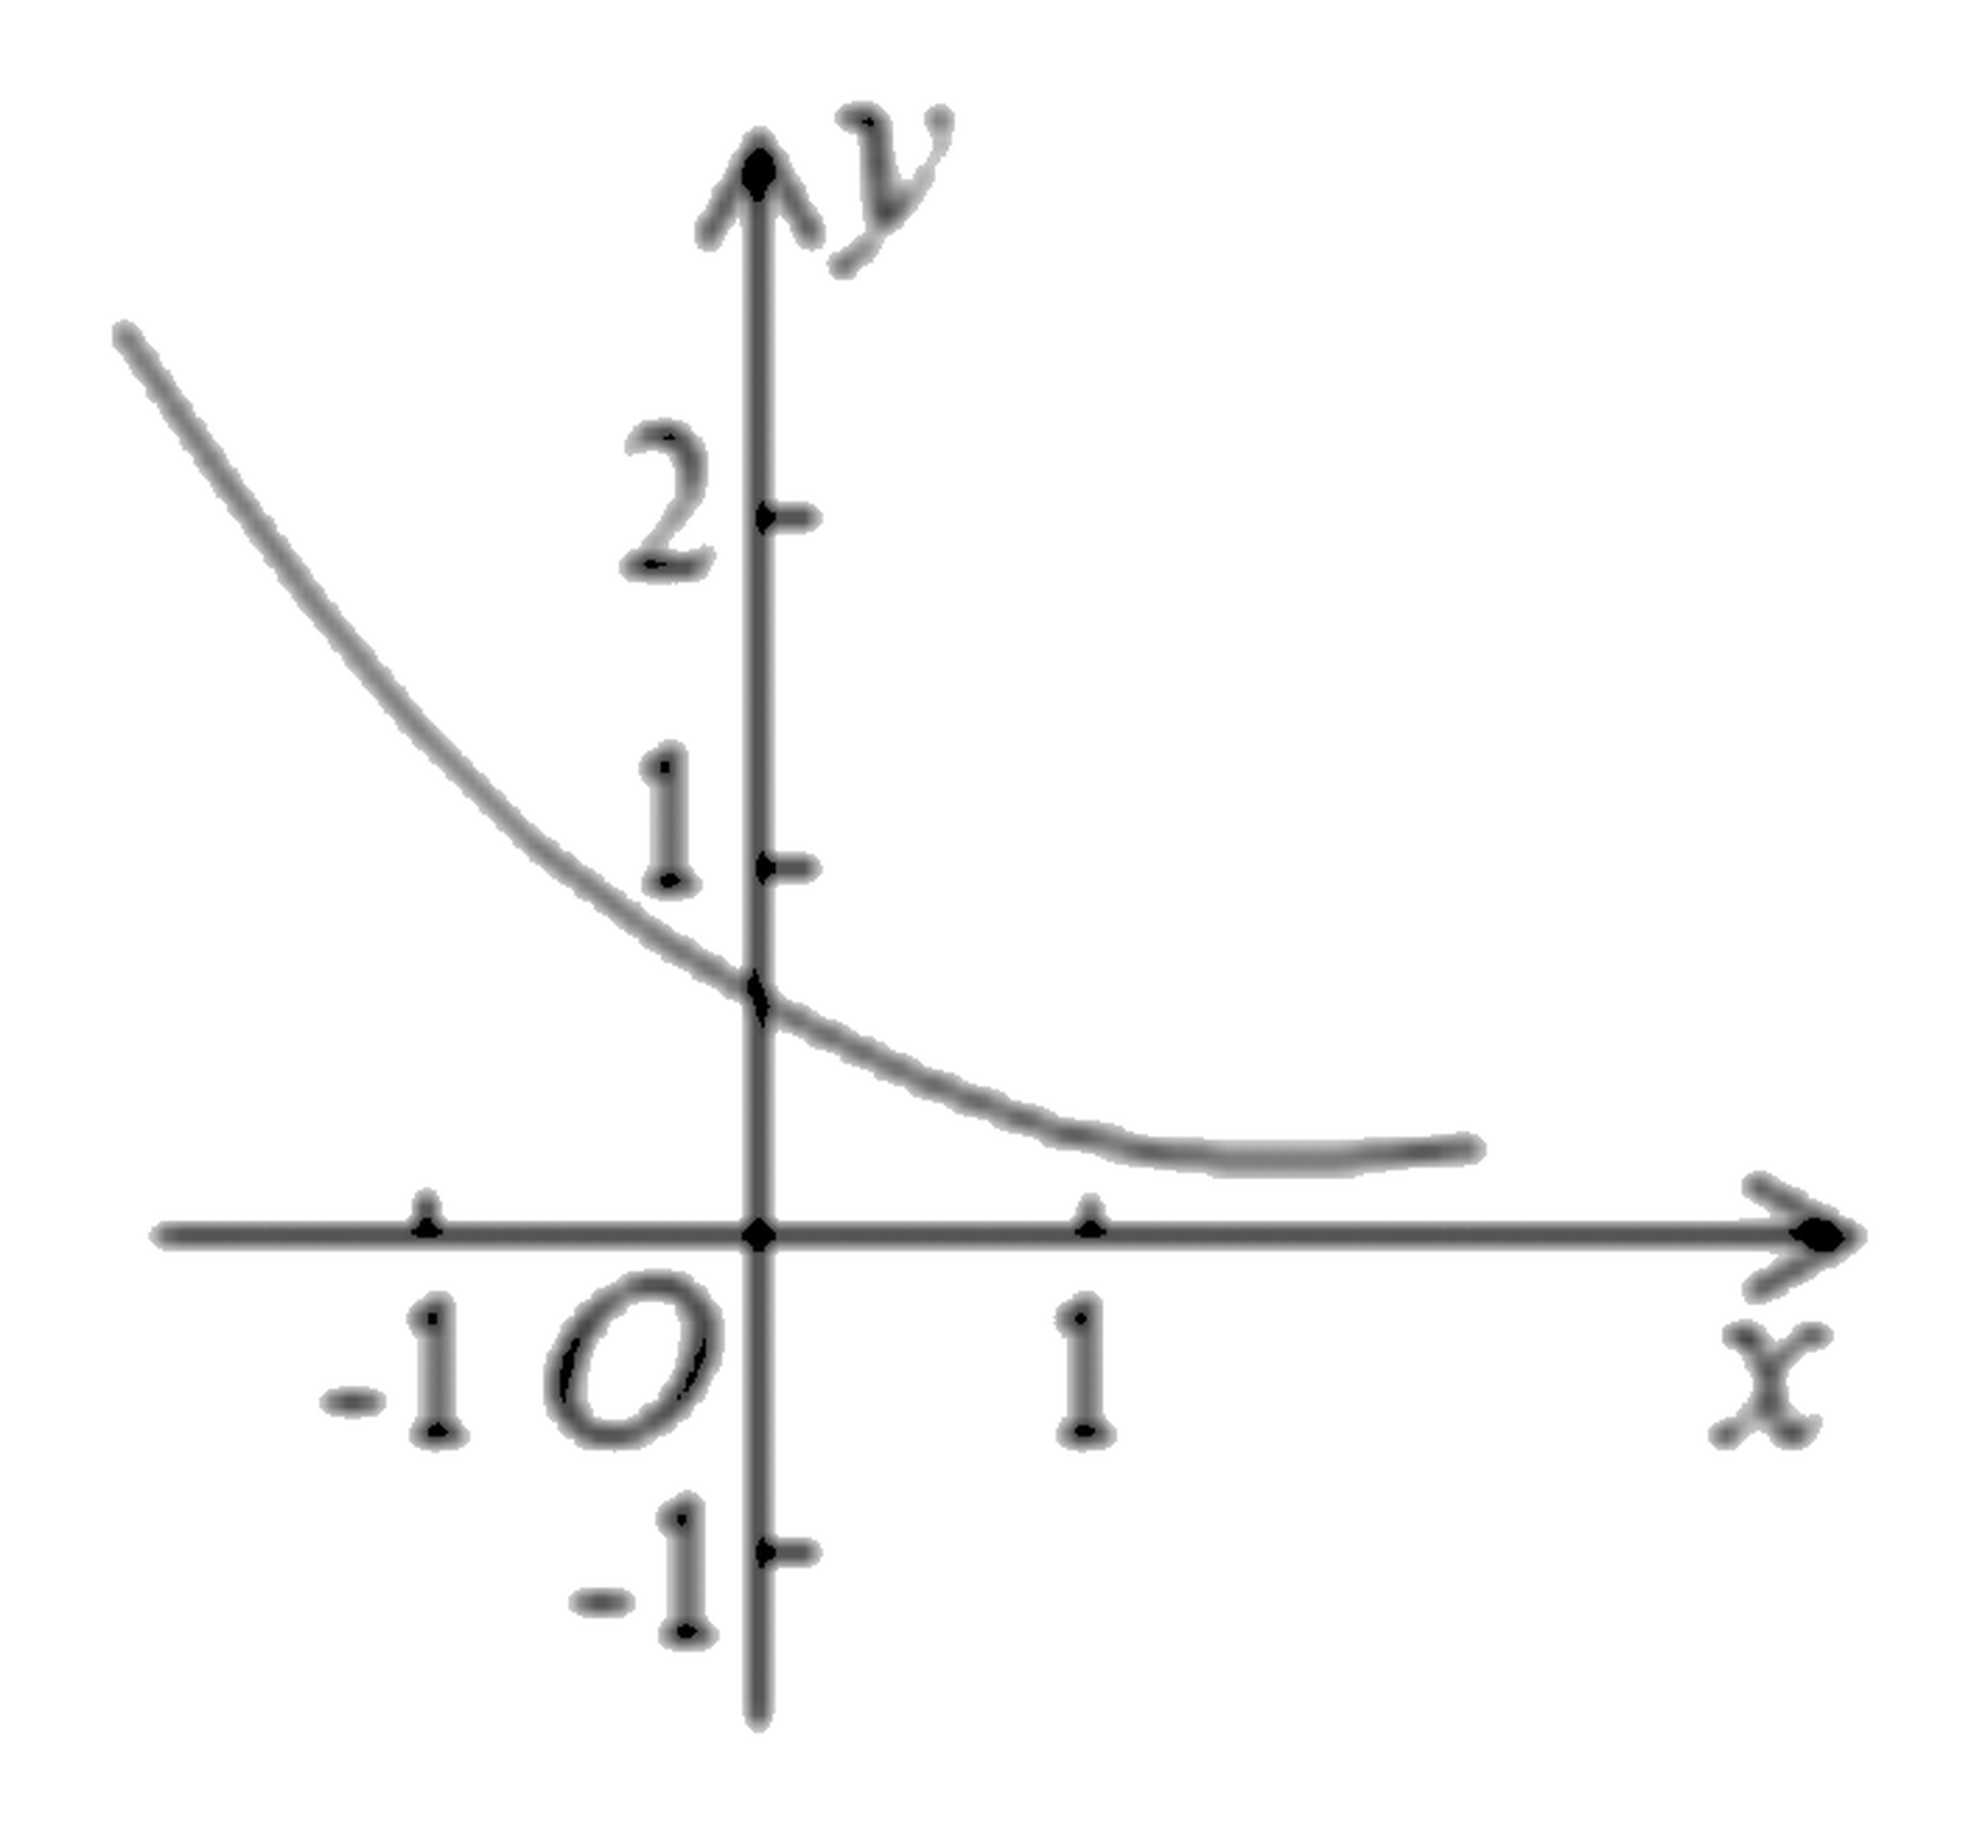
\includegraphics[width=0.30\textwidth]{figures/gao147_q15.png}
\end{center}

\ifanswer
\solbegin
\step{由图象从左到右下降得 $0<a<1$；}
\step{由图象与 $y$ 轴的交点得 $0<a^{-b}<1$，故 $b<0$；}
\step{故 $0<a<1$，$b<0$；故选 $D$.}
\solend
\fi

% === Q16 ===：位数新定义题（无弯引号，放大 04 页 z/q16_stem.png 确认）；四选项横排一行；解析 3 个印刷行
\item 数学运算是指在明晰运算对象的基础上，依据运算法则解决数学问题的素养. 因为运算，数的威力无限；没有运算，数就只是一个符号，对数运算与指数运算是两类重要的运算，对数的运算性质降低了运算的级别，简化了运算，在数学发展史上是伟大的成就. 而位数是指一个自然数有效位的个数，例如：$2^{10}=1024$，所以 $2^{10}$ 的位数为 4. 请你运用所学过的对数运算的知识，估计 $2025^{2026}$ 的位数是\mbox{（\quad）}

\keepwithprev
A. 6697\qquad B. 6698\qquad C. 6699\qquad D. 6700

\ifanswer
\solbegin
\step{设 $2025^{2026}=t$，所以 $\lg t=2026\lg2025$，}
\step{因为 $\lg2025\approx3.3064$，所以 $\lg t\approx6698.8$，}
\step{所以 $t\approx10^{6698.8}\in(10^{6698},10^{6699})$，所以 $2025^{2026}$ 的位数为 6699. 故选 $C$.}
\solend
\fi

\end{enumerate}

\bigsec{三、解答题}

\begin{enumerate}
\setcounter{enumi}{16}

% === Q17 ===：题干＋解析均在 04 页；集合描述竖线 \mid、描述内半角逗号照录；
% 空集 \varnothing、子集 \subseteq（放大 04 页 z/subset_04_q17b.png 确认带下划线）、数集 \R；
% 解析 5 个印刷行，首行末"所以 A=(-∞,-2)∪(3,+∞)"原卷无标点，照录不补
\item 已知集合 $A=\left\{x\mid \dfrac{x+2}{x-3}>0,x\in\R\right\}$，$B=\{x\mid \lvert x-2a\rvert\leqslant2,x\in\R\}$.

(1) 若 $a=1$，求 $A\cap B$；

(2) 若 $A\cap B=\varnothing$，求实数 $a$ 的取值范围.

\ifanswer
\solbegin
\step{由 $\dfrac{x+2}{x-3}>0$，得 $x<-2$ 或 $x>3$，所以 $A=(-\infty,-2)\cup(3,+\infty)$}
\step{(1) 当 $a=1$ 时，$B=\{x\mid \lvert x-2\rvert\leqslant2\}=[0,4]$，于是 $A\cap B=(3,4]$；}
\step{(2) $B=[2a-2,2a+2]$，}
\step{则 $A\cap B=\varnothing\Leftrightarrow[2a-2,2a+2]\subseteq[-2,3]\Leftrightarrow\begin{cases}2a-2\geqslant-2\\2a+2\leqslant3\end{cases}\Leftrightarrow0\leqslant a\leqslant\dfrac{1}{2}$，}
\step{所以实数 $a$ 的取值范围为 $\left[0,\dfrac{1}{2}\right]$.}
\solend
\fi

% === Q18 ===：氟化物／臭氧应用题；"氟化物""（如冰箱等）"全角夹注照录（放大 05 页 z/q18_line1.png 确认）；
% 关系式 $Q=Q_0e^{-0.0025t}$ 原卷独立一行，按一段照录；解析 6 个印刷行
\item 有些家用电器（如冰箱等）使用了氟化物，氟化物的释放破坏了大气上层的臭氧层，使臭氧含量 $Q$ 呈指数函数型变化，在氟化物排放量维持某种水平时，具有关系式

$Q=Q_0e^{-0.0025t}$，其中 $Q_0$ 是臭氧的初始量.

(1) 随时间 $t$ 的增加，臭氧的含量是增加还是减少？

(2) 试估计多少年以后将会有一半的臭氧消失.（用计算器计算）

\ifanswer
\solbegin
\step{(1) 对于函数 $Q=Q_0e^{-0.0025t}$，显然 $Q>0$，}
\step{任取 $t_1$、$t_2\in(0,+\infty)$，且 $t_1<t_2$，则 $t_2-t_1>0$，}
\step{所以 $\dfrac{Q_1}{Q_2}=\dfrac{Q_0e^{-0.0025t_1}}{Q_0e^{-0.0025t_2}}=e^{-0.0025(t_1-t_2)}=e^{0.0025(t_2-t_1)}>e^0=1$，所以 $Q_1>Q_2$，}
\step{故随着时间 $t$ 的增加，臭氧的含量是减少的；}
\step{(2) 令 $\dfrac{Q}{Q_0}=\dfrac{1}{2}$，即 $\dfrac{Q_0e^{-0.0025t}}{Q_0}=e^{-0.0025t}=\dfrac{1}{2}$，得 $-0.0025t=\ln\dfrac{1}{2}\approx-0.6931$，}
\step{解得 $t\approx277$，故估计 277 年以后将会有一半的臭氧消失.}
\solend
\fi

% === Q19 ===：题干用"图像"、解析两处用"图象"逐处照录不统一（05 页）；数集 \Z；
% 题干＋解析前 4 行在 05 页、解析后 3 行在 06 页；解析共 7 个印刷行
\item 已知幂函数 $f(x)=x^{-m^2+4m}(m\in\Z)$ 的图像关于 $y$ 轴对称，且在区间 $(0,+\infty)$ 上是严格增函数.

(1) 求 $m$ 的值；

(2) 求满足不等式 $(2a+1)^m<(a+1)^m$ 的实数 $a$ 的取值范围.

\ifanswer
\solbegin
\step{(1) 由题意得 $-m^2+4m>0$，解得 $0<m<4$，}
\step{因为 $m\in\Z$，所以 $m=1$ 或 $m=2$ 或 $m=3$.}
\step{当 $m=1$ 或 $m=3$ 时，$f(x)=x^3$，图象关于原点对称，不合题意；}
\step{当 $m=2$ 时，$f(x)=x^4$，图象关于 $y$ 轴对称，符合题意，所以 $m=2$.}
\step{(2) 代入 $m=2$，不等式为 $(2a+1)^2<(a+1)^2$，}
\step{得 $(2a+1)^2-(a+1)^2=a(3a+2)<0$，因此 $-\dfrac{2}{3}<a<0$，}
\step{所求范围为 $\left(-\dfrac{2}{3},0\right)$.}
\solend
\fi

% === Q20 ===：指数函数题，题干用"图像"；(3) 长求和式（分数 1/2026、1011/2026、2011/2026、
% 15/2026、1015/2026、2025/2026 放大 06 页 z/q20_sum_06a.png 确认）；题干在 06 页、
% 解析前 6 行在 06 页下半、后 6 行在 07 页上半；解析共 12 个印刷行
\item 已知指数函数 $y=a^x$（$a>0,a\ne1$）的图像经过点 $(1,4)$.

(1) 求实数 $a$ 的值；

(2) 若 $f(x)=(a^x)^2-2\cdot a^x-8$，当 $x\in\R$ 时，不等式 $f(x)>m\cdot4^x-12$ 恒成立，求 $m$ 的取值范围；

(3) 记 $g(x)=\dfrac{1}{a^x+2}$，求证：$g(x)+g(1-x)$ 为定值，并求 $g(0)+g\left(\dfrac{1}{2026}\right)+g\left(\dfrac{1011}{2026}\right)+g\left(\dfrac{2011}{2026}\right)+g\left(\dfrac{1}{2}\right)+g\left(\dfrac{15}{2026}\right)+g\left(\dfrac{1015}{2026}\right)+g\left(\dfrac{2025}{2026}\right)+g(1)$ 的值.

\ifanswer
\solbegin
\step{(1) 将 $(1,4)$ 代入 $y=a^x$，得 $a^1=4$，即 $a=4$.}
\step{(2) 令 $t=4^x$，当 $x\in\R$ 时，$t$ 取遍所有正实数.}
\step{原不等式等价于 $t^2-2t-8>mt-12\Leftrightarrow m<t+\dfrac{4}{t}-2$，}
\step{由基本不等式，$t+\dfrac{4}{t}-2\geqslant2\sqrt{t\cdot\dfrac{4}{t}}-2=2$，}
\step{当且仅当 $t=\dfrac{4}{t}$，即 $t=2$ 时取等号，}
\step{因此原不等式恒成立的充要条件为 $m<2$，即 $m\in(-\infty,2)$.}
\step{(3) 对任意 $x\in\R$，令 $t=4^x>0$，则 $4^{1-x}=\dfrac{4}{t}$，}
\step{从而 $g(x)+g(1-x)=\dfrac{1}{t+2}+\dfrac{1}{\dfrac{4}{t}+2}=\dfrac{1}{t+2}+\dfrac{t}{2(t+2)}=\dfrac{1}{2}$，}
\step{因此 $g(x)+g(1-x)$ 为定值 $\dfrac{1}{2}$.}
\step{原式中，0 与 1、$\dfrac{1}{2026}$ 与 $\dfrac{2025}{2026}$、$\dfrac{1011}{2026}$ 与 $\dfrac{1015}{2026}$、$\dfrac{2011}{2026}$ 与 $\dfrac{15}{2026}$}
\step{分别配对，每对函数值之和均为 $\dfrac{1}{2}$，且 $g\left(\dfrac{1}{2}\right)=\dfrac{1}{4^{\frac12}+2}=\dfrac{1}{4}$，}
\step{所以所求和为 $4\cdot\dfrac{1}{2}+\dfrac{1}{4}=\dfrac{9}{4}$.}
\solend
\fi

% === Q21 ===：不动点新定义题；题干在 07 页、解析续 08／09 页，共 20 个印刷行；
% 判别式两形混用：08 页 (2) cases 内等腰偏高 \Delta、09 页 (3) 扁等边 \triangle，逐处照录不统一
% （放大 /tmp/gao147/z/delta_vs_triangle.png 并排确认）；数集 \R；\forall 照录；
% 第 6—8 行是原卷一个长算式折成的三个印刷行，按印刷行分三条 \step、不并折行
\item 对于二次函数 $y=mx^2+nx+t(m\ne0)$，若存在 $x_0\in\R$，使得 $mx_0^2+nx_0+t=x_0$ 成立，则称 $x_0$ 为二次函数 $y=mx^2+nx+t(m\ne0)$ 的不动点.

(1) 求二次函数 $y=x^2-x-3$ 的不动点；

(2) 若二次函数 $y=2x^2-(3+a)x+a-1$ 有两个不相等的不动点 $x_1$、$x_2$，且 $x_1$、$x_2>0$，求 $\dfrac{x_1}{x_2}+\dfrac{x_2}{x_1}$ 的最小值；

(3) 若对任意实数 $b$，二次函数 $y=ax^2+(b+1)x+(b-1)(a\ne0)$ 恒有不动点，求 $a$ 的取值范围.

\ifanswer
\solbegin
\step{(1) 令 $x^2-x-3=x$，即 $x^2-2x-3=0$，即 $(x-3)(x+1)=0$，}
\step{解得 $x_1=-1$，$x_2=3$，所以不动点为 $-1$ 和 $3$.}
\step{(2) 由题意，$2x^2-(3+a)x+a-1=x$ 有两个不相等的正实数根，}
\step{即方程 $2x^2-(4+a)x+a-1=0$ 有两个不相等的正实数根，}
\step{所以 $\begin{cases}\Delta=(4+a)^2-8(a-1)>0\\x_1+x_2=\dfrac{4+a}{2}>0\\x_1\cdot x_2=\dfrac{a-1}{2}>0\end{cases}$，解得 $a>1$，}% 判别式原卷印等腰偏高粗三角 $\Delta$（放大 08 页 z/delta_08_q21cases.png）
\step{所以 $\dfrac{x_1}{x_2}+\dfrac{x_2}{x_1}=\dfrac{x_1^2+x_2^2}{x_1\cdot x_2}=\dfrac{(x_1+x_2)^2-2x_1\cdot x_2}{x_1\cdot x_2}=\dfrac{(x_1+x_2)^2}{x_1\cdot x_2}-2$}
\step{$=\dfrac{\left(\dfrac{4+a}{2}\right)^2}{\dfrac{a-1}{2}}-2=\dfrac{\dfrac{(a+4)^2}{4}}{\dfrac{a-1}{2}}-2=\dfrac{(a-1+5)^2}{2(a-1)}-2$}
\step{$=\dfrac{(a-1)^2+10(a-1)+25}{2(a-1)}-2=\dfrac{a-1}{2}+\dfrac{25}{2(a-1)}+3$.}
\step{因为 $a>1$，所以 $a-1>0$，}
\step{所以 $\dfrac{a-1}{2}+\dfrac{25}{2(a-1)}+3\geqslant2\sqrt{\dfrac{a-1}{2}\cdot\dfrac{25}{2(a-1)}}+3=8$，}
\step{当且仅当 $\dfrac{a-1}{2}=\dfrac{25}{2(a-1)}$，即 $a=6$ 时等号成立，}
\step{所以 $\dfrac{x_1}{x_2}+\dfrac{x_2}{x_1}$ 的最小值为 $8$.}
\step{(3) 设 $f(x)=ax^2+(b+1)x+b-1$，}
\step{则方程 $f(x)=x$，可化为 $ax^2+(b+1)x+b-1=x$，}
\step{即 $ax^2+bx+b-1=0$，}
\step{由题意得一元二次方程 $ax^2+bx+b-1=0$ 有解，又 $a\ne0$，}
\step{所以方程 $ax^2+bx+b-1=0$ 的判别式 $\triangle=b^2-4a(b-1)\geqslant0$，}% 判别式原卷印扁等边细线三角 $\triangle$（放大 09 页 z/triangle_09_q21.png），与 (2) 高 $\Delta$ 混用、照录不统一
\step{即 $b^2-4ab+4a\geqslant0$，则该不等式对 $\forall b\in\R$ 恒成立，}
\step{则 $(4a)^2-4\times4a\leqslant0$，且 $a\ne0$，解得 $0<a\leqslant1$，}
\step{所以实数 $a$ 的取值范围是 $(0,1]$.}
\solend
\fi

\end{enumerate}

\end{document}
"
%
% ① 原始材料：微信公众号"魔都数学加油站"文章，连载"27学年高一147"，原文标题
% "27学年高一147——2026-2027年上海市华师大三附中高一上期中"；
% 原文链接：https://mp.weixin.qq.com/s/X_gPW1JWoTAl2Bky_xEEGw 。
% 正文为 9 张 PNG 页（01/06/08/09 为 2560×3620，02/03/04/05/07 为 4762×6735，
% 同一篇各页分辨率混排，逐页按各自分辨率裁图核对，别按预览比例换算裁框）。
% 体例：混合体例讲评版——19 题中 Q4/Q5/Q7/Q9 只印【答案】、无【解析】，其余 15 题印
% 【解析】（逐题核实，见 ② ②）。题目、答案、解析均据原图转录；卷面粉红色水印
% "魔都数学加油站"及公众号页脚未录入。
% 全卷插图清单（逐页通读 9 页确认）：仅 1 处题目配图——
%   · Q15 递减指数函数小坐标系（03 页右侧：坐标轴、y 轴刻度 2/1/-1、x 轴刻度 -1/1、
%     原点 O、x/y 轴标），为"图像如图所示"的题目配图（选择题选项旁），三版都出；
%     裁自 03 页去粉色水印、去色、4× LANCZOS 放大存 figures/gao147_q15.png；
%   其余 8 页逐页确认无其它题目配图、无【解析】内配图、无表格，
%   亦无"题干写如图而源码漏图"一处；Q12/Q17/Q21 的 cases 块为数学块（非图）。
%
% 卷首标题：原卷印作"2026-2027 年华师大三附中高一上期中"，年份区间按全稿惯例排 en dash；
% 原卷卷面未印副标题，本稿按同期中卷（高一140／141／143／144／145／146）知识模块口径
% 补出"集合与常用逻辑用语、不等式、函数"。
%
% 题号体例（逐页核实定稿）：本卷共 19 题——一、填空题 3—12（10 题）、
% 二、选择题 13—16（4 题）、三、解答题 17—21（5 题）。
% 三节分别 \setcounter{enumi}{2}／{12}／{16}。原卷从第 3 题起、无第 1、2 题，
% 本稿保留原题号；全卷无附加题节（Q21 解析末行"所以实数 a 的取值范围是 (0,1]."
% 为全卷收尾，09 页下半仅水印、无正文）。
%
% ② 与原卷的排版差异：
%   ① 原文从第 3 题起，本稿保留原题号；共 19 题三节；
%   ② 混合体例：原卷 Q4/Q5/Q7/Q9 只印【答案】、无【解析】（分别为 a≤0、(-1,2)、
%      真、(-∞,1)），按 高一140 第 5 题／高一145 Q3 成例提 \ans{}、不补造解析；
%      其余 15 题印【解析】，用 \solbegin…\solend，选择题答案在解析末句"故选 X"
%      （Q13 选 B、Q14 选 B、Q15 选 D、Q16 选 C，逐个放大原图核实）、题干括号
%      \mbox{（\quad）} 留空、不另提 \ans{}；填空／解答答案落在解析里；
%      答案版【答案】/【解析】标记数 = 19（4 个 \ans ＋ 15 个 \solbegin）= 全卷题数；
%   ③ 原卷卷面未印副标题，本稿按知识模块口径补出；
%   ④ 原卷填空横线按全稿惯例排 \blankline[4.4em]；选择题括号排 \mbox{（\quad）}、
%      选项段前按惯例加 \keepwithprev；Q14／Q15 四选项为 2×2 两印刷行（A/B 一行、
%      C/D 一行），用空行分段照录（非一行 \qquad、亦非竖排四行）；解答题不留作答区、
%      不加 \anspace（原卷为讲评版，与 129／131／132／133／136／140／141／143／144／145／146 同）；
%   ⑤ 数集：Q4"A∪B=R"、Q13"f(x)=x^3 在 R 上严格增"、Q17"x∈R"两处、
%      Q20"x∈R"两处、Q21"x_0∈R""∀b∈R"原卷印斜体或黑板粗体 R，按全稿惯例统一改 \R；
%      Q19"m∈Z"改 \Z；本卷未出现 N（\N^* 无对应处）。绝对值排 \lvert…\rvert，
%      集合描述竖线排 \mid；不等号按全稿惯例排 \leqslant／\geqslant（原卷印 \le／\ge 形，
%      【答案】a≤0 亦排 \leqslant）；空集 \varnothing（Q17 两处）；
%      子集 \subseteq（Q17 带下划线，放大 04 页确认）；本卷未出现 \subset／\subsetneq，
%      亦未出现补集上划线 \overline{}；\left…\right 不得拆到不同 $…$ 组；
%   ⑥ 子题标号 (1)(2)(3) 半角括号照录；cases 块整体算一个印刷行（Q3、Q12 一行内
%      两个 cases、Q17、Q21(2)）；本卷解析内无圈数字①②③（无 \text{①} 需求）；
%      数学式内 CJK 用 \text{}（本卷未见）；
%   ⑦ 题干中的中文弯引号按原卷照录：Q7 命题"若 A∪B=B，则 A∩B=A"与
%      (填 " 真 " 或 " 假 ")、Q10 (填 ">" "<" "≤" "或≥")，含引号内空格；
%      注释内一律 ASCII 引号；Q16 位数新定义题逐字放大确认无弯引号
%      （交办提示的"Q16 新定义题"举例未在本卷出现），未补造引号；
%   ⑧ 半角逗号在数学组之间是全稿惯例、非笔误（Q4"$A=(-\infty,0],B=[a,+\infty)$"、
%      Q5"$(a>0,a\ne1)$"、Q17 集合描述内"$>0,x\in R$""$\leqslant2,x\in R$"、
%      Q20 题干"$(a>0,a\ne1)$"、Q21"$y=mx^2+nx+t(m\ne0)$"等），逐处照录别改全角；
%      行末西文句点照录为 ASCII `.`；行中全角逗号／顿号照录；
%      Q7／Q10"(填…)"为半角括号、Q18"（如冰箱等）"为全角括号，逐处照录不统一；
%   ⑨ "图像／图象"逐处照录不统一：题干 5 处用"图像"（Q5"图像恒过定点"、
%      Q9"图像位于直线 y=x 的下方"、Q15"的图像如图所示"、Q19"的图像关于 y 轴对称"、
%      Q20"的图像经过点"），解析 4 处用"图象"（Q15"由图象从左到右下降"
%      "由图象与 y 轴的交点"、Q19"图象关于原点对称""图象关于 y 轴对称"），逐处核、不统一；
%   ⑩ 判别式 Δ/△ 混用是照录项：Q21(2) 解析 cases 块"Δ=(4+a)²−8(a−1)>0"
%      印等腰偏高粗三角 \Delta，Q21(3) 解析"判别式△=b²−4a(b−1)≥0"
%      印扁等边细线三角 \triangle，逐处放大判断、照录不得统一
%      （参照 高一142／144／145 头注④口径，详见 ④）；
%   ⑪ 一条 \step = 原卷解析的一个印刷行，cases 块整体算一个印刷行；别把原卷折行
%      并起来、别把一行拆多条。Q10 七行（跨 01→02 页）、Q12 七行（含一行两 cases）、
%      Q20 十二行（含"原式中…2011/2026 与 15/2026／分别配对…"折行两行）、
%      Q21 二十行（含第 6—8 行一个长算式折成三印刷行、含 cases）均按印刷行逐条断，
%      不丢行；
%   ⑫ 配图：逐页通读 9 页确认全卷仅 Q15 一处题目配图（见 ①），三版都出、
%      \includegraphics[width=0.30\textwidth]；图块较小，未加 \needvspace 大图块守卫
%      （仅 \bigsec 自带 \needvspace{3\baselineskip}）；三版切页审计均"合计异常：无"；
%   ⑬ 跨页续印按题合并：Q3—Q9 在 01 页（Q10 题干在 01 页末、解析首行亦在 01 页末）；
%      Q10 解析续 02 页 6 行、Q11 在 02 页、Q12 题干＋解析前 4 行在 02 页
%      （解析续 03 页 3 行）；"二、选择题"标题与 Q13、Q14、Q15 题干＋解析前 2 行在 03 页
%      （Q15 配图在 03 页右侧）；Q15 解析末行与 Q16、"三、解答题"标题、Q17 在 04 页；
%      Q18 在 05 页、Q19 题干＋解析前 4 行在 05 页（解析续 06 页 3 行）；
%      Q20 题干＋解析前 6 行在 06 页（解析续 07 页 6 行）、Q21 题干＋解析前 3 行在 07 页；
%      Q21 解析续 08 页 13 行、续 09 页 4 行（09 页下半仅水印、无正文）。
%      本稿按题连排，不丢行、不并折行；
%   ⑭ 原卷解析内无红色"法一／法二"之类小标题，故本卷无 \stepm；
%      水印"魔都数学加油站"红色不录入。
%
% ③ 行数复核：一条 \step／\stepm = 原卷解析的一个印刷行，cases 块作一个印刷行计。
%   逐题数（主会话逐页核对定稿）：Q3：1；Q4：0（只印【答案】、提 \ans{}，不计入 \step 账）；
%   Q5：0；Q6：1；Q7：0；Q8：2；Q9：0；Q10：7；Q11：4；Q12：7；Q13：6；Q14：4；
%   Q15：3；Q16：3；Q17：5；Q18：6；Q19：7；Q20：12；Q21：20。
%   合计 88 条 \step（本卷无 \stepm：解析内无红色"法一／法二"类小标题），
%   与原卷逐题印刷行相等。全卷 15 题设 \solbegin…\solend ＋ 4 题一处 \ans{}，
%   答案版【答案】/【解析】标记数 = 19 = 全卷题数。
%
% ④ 判别式／子集符号结论（逐处放大原图照录、不得统一，主会话像素级复核）：
%   判别式全卷 2 处、两形混用逐处照录不统一（参照 高一142／144 头注④口径）：
%     · Q21(2) 解析 cases 块"Δ=(4+a)²−8(a−1)>0" 原卷印等腰偏高粗三角
%       （高>宽、粗笔画），照录 \Delta（放大 08 页 /tmp/gao147/z/delta_08_q21cases.png
%       与 z/delta_vs_triangle.png 左图确认）；
%     · Q21(3) 解析"判别式△=b²−4a(b−1)≥0" 原卷印扁等边细线三角
%       （宽≈高、细线），照录 \triangle（放大 09 页 /tmp/gao147/z/triangle_09_q21.png
%       与 z/delta_vs_triangle.png 右图并排确认）。
%   子集／补集：Q17 解析"[2a−2,2a+2]⊆[−2,3]" 原卷印带下划线 ⊆，照录 \subseteq
%     （放大 04 页 /tmp/gao147/z/subset_04_q17b.png 确认）；Q17"A∩B=∅"空集 \varnothing；
%     集合描述竖线 \mid（Q10 M、Q12 解集、Q17 A/B）；并集 \cup（Q4、Q17）、
%     交集 \cap（Q7、Q17）、不属于 \notin（Q10）；数集 \R／\Z 归一见 ② ⑤。
%   本卷未出现 \subset／\subsetneq，未出现补集上划线 \overline{}。
%
% ⑤ 存疑照录（放大原图确认，照录未改、正文对应处另有 % 注）：
%   1. Q4/Q5/Q7/Q9 只印【答案】、无【解析】，按成例提 \ans{}、不补造解析
%      （混合体例逐题核实，见 ② ②）。
%   2. Q21(2) 判别式高 \Delta 与 Q21(3) 判别式扁 \triangle 两形混用，
%      逐处照录不统一（见 ④）。
%   3. "图像／图象"题干 5 处"图像"、解析 4 处"图象"，逐处照录不统一（见 ② ⑨）。
%   4. Q7／Q10"(填…)"半角括号与 Q18"（如冰箱等）"全角括号，逐处照录不统一。
%   5. Q16 位数新定义题逐字放大确认无弯引号（交办提示的"Q16 新定义题"举例
%      未在本卷出现），未补造引号；全卷弯引号仅 Q7、Q10 两处。
%   6. Q17 解析首行末"所以 A=(-∞,-2)∪(3,+∞)"、Q20(3) 解析"…2011/2026 与 15/2026"
%      行末原卷均无标点，照录未补；Q21(2) 第 6—8 行一个长算式折成三印刷行，
%      按印刷行分三条 \step、不并折行。
%   全卷除此 6 类外未发现其它笔误／自相矛盾处。
%
% ⑥ 跨页续印按题合并说明：见 ② ⑬。
%
\documentclass[a4paper,11pt]{article}
\usepackage{common}

\begin{document}

\examtitlest[3]{2026--2027 年华师大三附中高一上期中}{集合与常用逻辑用语、不等式、函数}

\bigsec{一、填空题}

\begin{enumerate}
\setcounter{enumi}{2}

% === Q3 ===：印【解析】，1 个印刷行（cases 块整体算一行）
\item 函数 $y=(a^2-5a+7)a^x+6-2a$ 是指数函数，则 $a$ 的值为\blankline[4.4em].

\ifanswer
\solbegin
\step{由题意得 $\begin{cases}a^2-5a+7=1\\6-2a=0\end{cases}$，解得 $a=3$.}
\solend
\fi

% === Q4 ===：原卷只印【答案】、无【解析】，按 高一140 第 5 题／高一145 Q3 成例提 \ans{}、不补造解析；
% 题干数学组内半角逗号 $A=(-\infty,0],B=[a,+\infty)$ 照录（放大 01 页 z/q4_stem.png 确认）
\item 已知 $A=(-\infty,0],B=[a,+\infty)$，且 $A\cup B=\R$，则实数 $a$ 的取值范围为\blankline[4.4em].

\ifanswer
\ans{$a\leqslant0$}
\fi

% === Q5 ===：只印【答案】；题干"图像"照录（放大 01 页 z/q5_stem.png 确认）；
% 数学组内半角逗号 $(a>0,a\ne1)$ 照录
\item 函数 $y=a^{x+1}+1(a>0,a\ne1)$ 的图像恒过定点\blankline[4.4em].

\ifanswer
\ans{$(-1,2)$}
\fi

% === Q6 ===：印【解析】，1 个印刷行
\item 已知方程 $x^2+2x-4=0$ 的两个根为 $x_1$、$x_2$，则 $x_1^2+x_2^2$ 的值为\blankline[4.4em].

\ifanswer
\solbegin
\step{$x_1^2+x_2^2=(x_1+x_2)^2-2x_1x_2=4+8=12$.}
\solend
\fi

% === Q7 ===：只印【答案】；中文弯引号"若 A∪B=B，则 A∩B=A"与(填 " 真 " 或 " 假 ")内的空格照录
% （放大 01 页 z/q7_quotes_7x.png、z/q7_tail.png 确认，括号为半角）
\item 命题 “若 $A\cup B=B$，则 $A\cap B=A$” 为\blankline[4.4em]命题(填 “ 真 ” 或 “ 假 ”).

\ifanswer
\ans{真}
\fi

% === Q8 ===：印【解析】，2 个印刷行；不等号按全稿惯例 \geqslant／\leqslant
\item 已知正实数 $a$、$b$ 满足 $a+4b=1$，则 $ab$ 的最大值为\blankline[4.4em].

\ifanswer
\solbegin
\step{$a+4b\geqslant2\sqrt{a\cdot4b}\Rightarrow ab\leqslant\dfrac{1}{16}$，当且仅当 $a=4b=\dfrac{1}{2}$ 时取等号，}
\step{则 $ab$ 的最大值为 $\dfrac{1}{16}$.}
\solend
\fi

% === Q9 ===：只印【答案】；题干"图像"照录（放大 01 页 hi_01_2 确认）
\item 若幂函数 $y=x^s$ 在 $x>1$ 时的图像位于直线 $y=x$ 的下方，则 $s$ 的取值范围是\blankline[4.4em].

\ifanswer
\ans{$(-\infty,1)$}
\fi

% === Q10 ===：印【解析】，共 7 个印刷行（题在 01 页末起 1 行、续 02 页 6 行）；
% 题干跨两印刷行"则 |ab|+1 ____ |a|+|b|（填…）"按一句连排；(填…)为半角括号、引号内空格照录
\item 已知不等式 $\lvert2x+1\rvert+\lvert2x-1\rvert<4$ 的解集为 $M$. 设实数 $a\in M$，$b\notin M$，则 $\lvert ab\rvert+1$\blankline[4.4em] $\lvert a\rvert+\lvert b\rvert$(填 “$>$”，“$<$”，“$\leqslant$” “或$\geqslant$”).

\ifanswer
\solbegin
\step{当 $x<-\dfrac{1}{2}$ 时，不等式化为 $-2x-1+1-2x<4$，即 $x>-1$，所以 $-1<x<-\dfrac{1}{2}$；}
\step{当 $-\dfrac{1}{2}\leqslant x\leqslant\dfrac{1}{2}$ 时，不等式化为 $2x+1-2x+1<4$，即 $2<4$，所以 $-\dfrac{1}{2}\leqslant x\leqslant\dfrac{1}{2}$；}
\step{当 $x>\dfrac{1}{2}$ 时，不等式化为 $2x+1+2x-1<4$，即 $x<1$，所以 $\dfrac{1}{2}<x<1$；}
\step{综上，$M=\{x\mid -1<x<1\}$.}
\step{因为 $a\in M$，$b\notin M$，所以 $\lvert a\rvert<1$，$\lvert b\rvert\geqslant1$.}
\step{而 $\lvert ab\rvert+1-(\lvert a\rvert+\lvert b\rvert)=\lvert ab\rvert+1-\lvert a\rvert-\lvert b\rvert=(\lvert a\rvert-1)(\lvert b\rvert-1)$，}
\step{所以 $\lvert ab\rvert+1\leqslant\lvert a\rvert+\lvert b\rvert$.}
\solend
\fi

% === Q11 ===：印【解析】，4 个印刷行（02 页）
\item 已知 $m>1$，$n>1$，$\lg m=\log_n100$，则 $mn$ 的最小值为\blankline[4.4em].

\ifanswer
\solbegin
\step{由 $m>1$，$n>1$，得 $\lg m>0$，$\lg n>0$，}
\step{因为 $\lg m=\log_n100=\dfrac{\lg100}{\lg n}=\dfrac{2}{\lg n}$，所以 $\lg m\cdot\lg n=2$，}
\step{所以 $\lg(mn)=\lg m+\lg n\geqslant2\sqrt{\lg m\cdot\lg n}=2\sqrt2$，}
\step{当且仅当 $m=n=10^{\sqrt2}$ 时取等号，则 $mn\geqslant10^{2\sqrt2}$，即 $mn$ 的最小值为 $10^{2\sqrt2}$.}
\solend
\fi

% === Q12 ===：印【解析】，共 7 个印刷行（02 页 4 行、03 页 3 行）；
% 第 3 行"则 [cases]，得 [cases]，"两个 cases 块同属一个印刷行，整体作一条 \step（照 高一146 Q11 成例）
\item 已知关于 $x$ 的不等式 $ax^2+bx+c\leqslant1$ 的解集为 $\{x\mid -1\leqslant x\leqslant3\}$. 若关于 $x$ 的不等式 $ax^2+(b-1)x+c-2\leqslant0$ 有且仅有 8 个整数解，则实数 $a$ 的取值范围是\blankline[4.4em].

\ifanswer
\solbegin
\step{由已知关于 $x$ 的不等式 $ax^2+bx+c\leqslant1$ 的解集为 $\{x\mid -1\leqslant x\leqslant3\}$，}
\step{得 $a>0$，且方程 $ax^2+bx+c-1=0$ 的两根分别为 $-1$ 和 $3$，}
\step{则 $\begin{cases}-1+3=-\dfrac{b}{a}\\-1\times3=\dfrac{c-1}{a}\end{cases}$，得 $\begin{cases}b=-2a\\c=1-3a\end{cases}$，}
\step{不等式 $ax^2+(b-1)x+c-2\leqslant0$ 等价于 $ax^2-(2a+1)x-(3a+1)\leqslant0$，}
\step{即 $\left[x-\left(3+\dfrac{1}{a}\right)\right](x+1)\leqslant0$，解得 $-1\leqslant x\leqslant3+\dfrac{1}{a}$，}
\step{因为关于 $x$ 的不等式 $ax^2+(b-1)x+c-2\leqslant0$ 有且仅有 8 个整数解，}
\step{因此 $6\leqslant3+\dfrac{1}{a}<7$，即 $3\leqslant\dfrac{1}{a}<4$，解得 $\dfrac{1}{4}<a\leqslant\dfrac{1}{3}$，所以 $a$ 的取值范围为 $\left(\dfrac{1}{4},\dfrac{1}{3}\right]$.}
\solend
\fi

\end{enumerate}

\bigsec{二、选择题}

\begin{enumerate}
\setcounter{enumi}{12}

% === Q13 ===：题干＋选项＋解析均在 03 页；四选项横排一行；解析 6 个印刷行，末句"故选 B."
\item $a<b<0$，则下列不等式能成立的是\mbox{（\quad）}

\keepwithprev
A. $\dfrac{a}{b}<1$\qquad B. $\lvert a\rvert>-b$\qquad C. $\dfrac{1}{a}<\dfrac{1}{b}$\qquad D. $b^3<a^3$

\ifanswer
\solbegin
\step{对于 $A$，令 $a=-4$，$b=-3$，满足 $a<b<0$，但 $\dfrac{a}{b}>1$，故 $A$ 错误，}
\step{对于 $B$，因为 $a<b<0$，所以 $-a>-b>0$，即 $\lvert a\rvert>-b$，故 $B$ 正确，}
\step{对于 $C$，令 $a=-4$，$b=-3$，满足 $a<b<0$，但 $\dfrac{1}{a}>\dfrac{1}{b}$，故 $C$ 错误，}
\step{对于 $D$，$f(x)=x^3$ 在 $\R$ 上严格增，因为 $a<b$，所以 $f(a)<f(b)$，}
\step{即 $a^3<b^3$，故 $D$ 错误.}
\step{故选 $B$.}
\solend
\fi

% === Q14 ===：四选项原卷为 2×2 两印刷行（A/B 一行、C/D 一行），用空行分段照录；解析 4 个印刷行
\item 已知 $a$、$b$ 为实数，若 $\alpha:ab=0$，$\beta:a^2+\sqrt{b}=0$，则 $\alpha$ 是 $\beta$ 的\mbox{（\quad）}

\keepwithprev
A. 充分不必要条件\qquad\qquad B. 必要不充分条件

C. 充要条件\qquad\qquad D. 既不充分也不必要条件

\ifanswer
\solbegin
\step{$\beta:a^2+\sqrt{b}=0$，所以 $a=0$ 且 $b=0$，}
\step{由 $a=0$，$b=0\Rightarrow ab=0$，反之不成立.}
\step{所以 $ab=0$ 是 $a=0$，$b=0$ 的必要不充分条件，即 $\alpha$ 是 $\beta$ 的必要不充分条件，}
\step{故选 $B$.}
\solend
\fi

% === Q15 ===：题目配图（03 页右侧小坐标系），三版都出；题干用"图像"、解析用"图象"逐处照录；
% 四选项 2×2 两印刷行；解析 3 个印刷行（03 页 2 行、04 页 1 行，末句"故选 D."与前行同一印刷行）
\item 函数 $f(x)=a^{x-b}$ 的图像如图所示，其中 $a$、$b$ 为常数，则下列结论正确的是\mbox{（\quad）}

\keepwithprev
A. $a>1$，$b<0$\qquad\qquad B. $a>1$，$b>0$

C. $0<a<1$，$b>0$\qquad\qquad D. $0<a<1$，$b<0$

\begin{center}
% 递减指数函数小坐标系图取 03 页右侧，去粉色水印、去色、4× LANCZOS 放大；题目配图三版都出
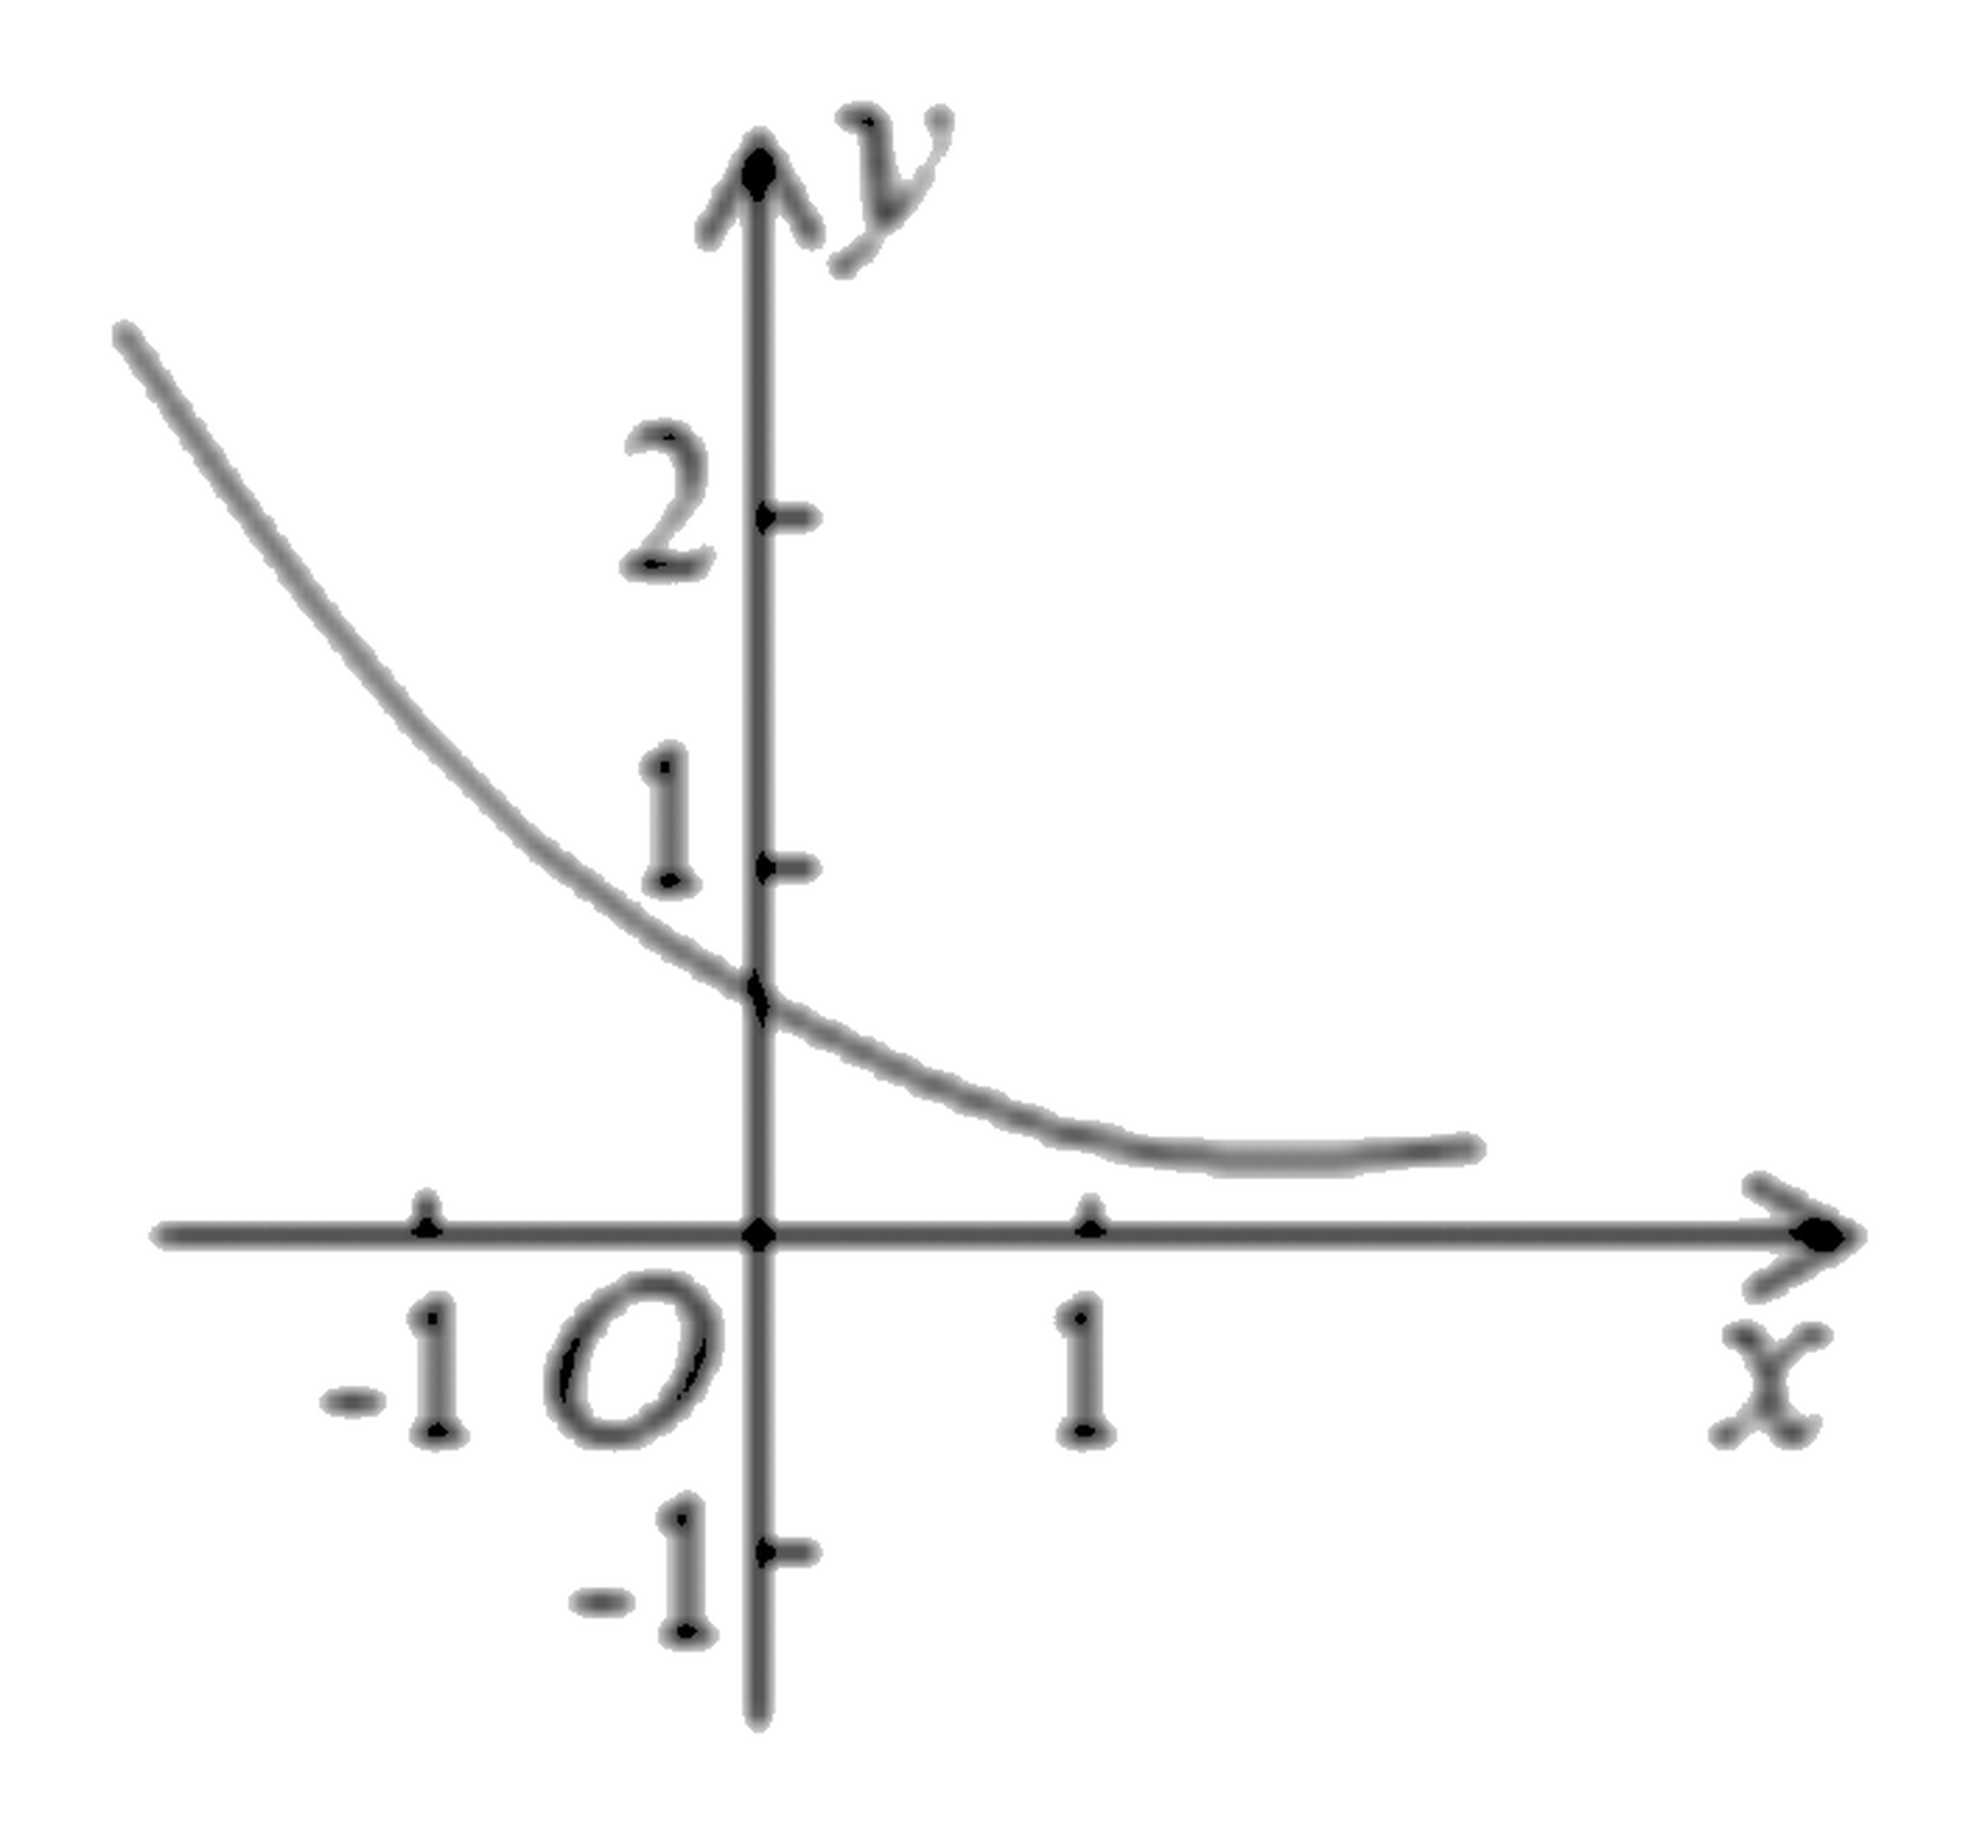
\includegraphics[width=0.30\textwidth]{figures/gao147_q15.png}
\end{center}

\ifanswer
\solbegin
\step{由图象从左到右下降得 $0<a<1$；}
\step{由图象与 $y$ 轴的交点得 $0<a^{-b}<1$，故 $b<0$；}
\step{故 $0<a<1$，$b<0$；故选 $D$.}
\solend
\fi

% === Q16 ===：位数新定义题（无弯引号，放大 04 页 z/q16_stem.png 确认）；四选项横排一行；解析 3 个印刷行
\item 数学运算是指在明晰运算对象的基础上，依据运算法则解决数学问题的素养. 因为运算，数的威力无限；没有运算，数就只是一个符号，对数运算与指数运算是两类重要的运算，对数的运算性质降低了运算的级别，简化了运算，在数学发展史上是伟大的成就. 而位数是指一个自然数有效位的个数，例如：$2^{10}=1024$，所以 $2^{10}$ 的位数为 4. 请你运用所学过的对数运算的知识，估计 $2025^{2026}$ 的位数是\mbox{（\quad）}

\keepwithprev
A. 6697\qquad B. 6698\qquad C. 6699\qquad D. 6700

\ifanswer
\solbegin
\step{设 $2025^{2026}=t$，所以 $\lg t=2026\lg2025$，}
\step{因为 $\lg2025\approx3.3064$，所以 $\lg t\approx6698.8$，}
\step{所以 $t\approx10^{6698.8}\in(10^{6698},10^{6699})$，所以 $2025^{2026}$ 的位数为 6699. 故选 $C$.}
\solend
\fi

\end{enumerate}

\bigsec{三、解答题}

\begin{enumerate}
\setcounter{enumi}{16}

% === Q17 ===：题干＋解析均在 04 页；集合描述竖线 \mid、描述内半角逗号照录；
% 空集 \varnothing、子集 \subseteq（放大 04 页 z/subset_04_q17b.png 确认带下划线）、数集 \R；
% 解析 5 个印刷行，首行末"所以 A=(-∞,-2)∪(3,+∞)"原卷无标点，照录不补
\item 已知集合 $A=\left\{x\mid \dfrac{x+2}{x-3}>0,x\in\R\right\}$，$B=\{x\mid \lvert x-2a\rvert\leqslant2,x\in\R\}$.

(1) 若 $a=1$，求 $A\cap B$；

(2) 若 $A\cap B=\varnothing$，求实数 $a$ 的取值范围.

\ifanswer
\solbegin
\step{由 $\dfrac{x+2}{x-3}>0$，得 $x<-2$ 或 $x>3$，所以 $A=(-\infty,-2)\cup(3,+\infty)$}
\step{(1) 当 $a=1$ 时，$B=\{x\mid \lvert x-2\rvert\leqslant2\}=[0,4]$，于是 $A\cap B=(3,4]$；}
\step{(2) $B=[2a-2,2a+2]$，}
\step{则 $A\cap B=\varnothing\Leftrightarrow[2a-2,2a+2]\subseteq[-2,3]\Leftrightarrow\begin{cases}2a-2\geqslant-2\\2a+2\leqslant3\end{cases}\Leftrightarrow0\leqslant a\leqslant\dfrac{1}{2}$，}
\step{所以实数 $a$ 的取值范围为 $\left[0,\dfrac{1}{2}\right]$.}
\solend
\fi

% === Q18 ===：氟化物／臭氧应用题；"氟化物""（如冰箱等）"全角夹注照录（放大 05 页 z/q18_line1.png 确认）；
% 关系式 $Q=Q_0e^{-0.0025t}$ 原卷独立一行，按一段照录；解析 6 个印刷行
\item 有些家用电器（如冰箱等）使用了氟化物，氟化物的释放破坏了大气上层的臭氧层，使臭氧含量 $Q$ 呈指数函数型变化，在氟化物排放量维持某种水平时，具有关系式

$Q=Q_0e^{-0.0025t}$，其中 $Q_0$ 是臭氧的初始量.

(1) 随时间 $t$ 的增加，臭氧的含量是增加还是减少？

(2) 试估计多少年以后将会有一半的臭氧消失.（用计算器计算）

\ifanswer
\solbegin
\step{(1) 对于函数 $Q=Q_0e^{-0.0025t}$，显然 $Q>0$，}
\step{任取 $t_1$、$t_2\in(0,+\infty)$，且 $t_1<t_2$，则 $t_2-t_1>0$，}
\step{所以 $\dfrac{Q_1}{Q_2}=\dfrac{Q_0e^{-0.0025t_1}}{Q_0e^{-0.0025t_2}}=e^{-0.0025(t_1-t_2)}=e^{0.0025(t_2-t_1)}>e^0=1$，所以 $Q_1>Q_2$，}
\step{故随着时间 $t$ 的增加，臭氧的含量是减少的；}
\step{(2) 令 $\dfrac{Q}{Q_0}=\dfrac{1}{2}$，即 $\dfrac{Q_0e^{-0.0025t}}{Q_0}=e^{-0.0025t}=\dfrac{1}{2}$，得 $-0.0025t=\ln\dfrac{1}{2}\approx-0.6931$，}
\step{解得 $t\approx277$，故估计 277 年以后将会有一半的臭氧消失.}
\solend
\fi

% === Q19 ===：题干用"图像"、解析两处用"图象"逐处照录不统一（05 页）；数集 \Z；
% 题干＋解析前 4 行在 05 页、解析后 3 行在 06 页；解析共 7 个印刷行
\item 已知幂函数 $f(x)=x^{-m^2+4m}(m\in\Z)$ 的图像关于 $y$ 轴对称，且在区间 $(0,+\infty)$ 上是严格增函数.

(1) 求 $m$ 的值；

(2) 求满足不等式 $(2a+1)^m<(a+1)^m$ 的实数 $a$ 的取值范围.

\ifanswer
\solbegin
\step{(1) 由题意得 $-m^2+4m>0$，解得 $0<m<4$，}
\step{因为 $m\in\Z$，所以 $m=1$ 或 $m=2$ 或 $m=3$.}
\step{当 $m=1$ 或 $m=3$ 时，$f(x)=x^3$，图象关于原点对称，不合题意；}
\step{当 $m=2$ 时，$f(x)=x^4$，图象关于 $y$ 轴对称，符合题意，所以 $m=2$.}
\step{(2) 代入 $m=2$，不等式为 $(2a+1)^2<(a+1)^2$，}
\step{得 $(2a+1)^2-(a+1)^2=a(3a+2)<0$，因此 $-\dfrac{2}{3}<a<0$，}
\step{所求范围为 $\left(-\dfrac{2}{3},0\right)$.}
\solend
\fi

% === Q20 ===：指数函数题，题干用"图像"；(3) 长求和式（分数 1/2026、1011/2026、2011/2026、
% 15/2026、1015/2026、2025/2026 放大 06 页 z/q20_sum_06a.png 确认）；题干在 06 页、
% 解析前 6 行在 06 页下半、后 6 行在 07 页上半；解析共 12 个印刷行
\item 已知指数函数 $y=a^x$（$a>0,a\ne1$）的图像经过点 $(1,4)$.

(1) 求实数 $a$ 的值；

(2) 若 $f(x)=(a^x)^2-2\cdot a^x-8$，当 $x\in\R$ 时，不等式 $f(x)>m\cdot4^x-12$ 恒成立，求 $m$ 的取值范围；

(3) 记 $g(x)=\dfrac{1}{a^x+2}$，求证：$g(x)+g(1-x)$ 为定值，并求 $g(0)+g\left(\dfrac{1}{2026}\right)+g\left(\dfrac{1011}{2026}\right)+g\left(\dfrac{2011}{2026}\right)+g\left(\dfrac{1}{2}\right)+g\left(\dfrac{15}{2026}\right)+g\left(\dfrac{1015}{2026}\right)+g\left(\dfrac{2025}{2026}\right)+g(1)$ 的值.

\ifanswer
\solbegin
\step{(1) 将 $(1,4)$ 代入 $y=a^x$，得 $a^1=4$，即 $a=4$.}
\step{(2) 令 $t=4^x$，当 $x\in\R$ 时，$t$ 取遍所有正实数.}
\step{原不等式等价于 $t^2-2t-8>mt-12\Leftrightarrow m<t+\dfrac{4}{t}-2$，}
\step{由基本不等式，$t+\dfrac{4}{t}-2\geqslant2\sqrt{t\cdot\dfrac{4}{t}}-2=2$，}
\step{当且仅当 $t=\dfrac{4}{t}$，即 $t=2$ 时取等号，}
\step{因此原不等式恒成立的充要条件为 $m<2$，即 $m\in(-\infty,2)$.}
\step{(3) 对任意 $x\in\R$，令 $t=4^x>0$，则 $4^{1-x}=\dfrac{4}{t}$，}
\step{从而 $g(x)+g(1-x)=\dfrac{1}{t+2}+\dfrac{1}{\dfrac{4}{t}+2}=\dfrac{1}{t+2}+\dfrac{t}{2(t+2)}=\dfrac{1}{2}$，}
\step{因此 $g(x)+g(1-x)$ 为定值 $\dfrac{1}{2}$.}
\step{原式中，0 与 1、$\dfrac{1}{2026}$ 与 $\dfrac{2025}{2026}$、$\dfrac{1011}{2026}$ 与 $\dfrac{1015}{2026}$、$\dfrac{2011}{2026}$ 与 $\dfrac{15}{2026}$}
\step{分别配对，每对函数值之和均为 $\dfrac{1}{2}$，且 $g\left(\dfrac{1}{2}\right)=\dfrac{1}{4^{\frac12}+2}=\dfrac{1}{4}$，}
\step{所以所求和为 $4\cdot\dfrac{1}{2}+\dfrac{1}{4}=\dfrac{9}{4}$.}
\solend
\fi

% === Q21 ===：不动点新定义题；题干在 07 页、解析续 08／09 页，共 20 个印刷行；
% 判别式两形混用：08 页 (2) cases 内等腰偏高 \Delta、09 页 (3) 扁等边 \triangle，逐处照录不统一
% （放大 /tmp/gao147/z/delta_vs_triangle.png 并排确认）；数集 \R；\forall 照录；
% 第 6—8 行是原卷一个长算式折成的三个印刷行，按印刷行分三条 \step、不并折行
\item 对于二次函数 $y=mx^2+nx+t(m\ne0)$，若存在 $x_0\in\R$，使得 $mx_0^2+nx_0+t=x_0$ 成立，则称 $x_0$ 为二次函数 $y=mx^2+nx+t(m\ne0)$ 的不动点.

(1) 求二次函数 $y=x^2-x-3$ 的不动点；

(2) 若二次函数 $y=2x^2-(3+a)x+a-1$ 有两个不相等的不动点 $x_1$、$x_2$，且 $x_1$、$x_2>0$，求 $\dfrac{x_1}{x_2}+\dfrac{x_2}{x_1}$ 的最小值；

(3) 若对任意实数 $b$，二次函数 $y=ax^2+(b+1)x+(b-1)(a\ne0)$ 恒有不动点，求 $a$ 的取值范围.

\ifanswer
\solbegin
\step{(1) 令 $x^2-x-3=x$，即 $x^2-2x-3=0$，即 $(x-3)(x+1)=0$，}
\step{解得 $x_1=-1$，$x_2=3$，所以不动点为 $-1$ 和 $3$.}
\step{(2) 由题意，$2x^2-(3+a)x+a-1=x$ 有两个不相等的正实数根，}
\step{即方程 $2x^2-(4+a)x+a-1=0$ 有两个不相等的正实数根，}
\step{所以 $\begin{cases}\Delta=(4+a)^2-8(a-1)>0\\x_1+x_2=\dfrac{4+a}{2}>0\\x_1\cdot x_2=\dfrac{a-1}{2}>0\end{cases}$，解得 $a>1$，}% 判别式原卷印等腰偏高粗三角 $\Delta$（放大 08 页 z/delta_08_q21cases.png）
\step{所以 $\dfrac{x_1}{x_2}+\dfrac{x_2}{x_1}=\dfrac{x_1^2+x_2^2}{x_1\cdot x_2}=\dfrac{(x_1+x_2)^2-2x_1\cdot x_2}{x_1\cdot x_2}=\dfrac{(x_1+x_2)^2}{x_1\cdot x_2}-2$}
\step{$=\dfrac{\left(\dfrac{4+a}{2}\right)^2}{\dfrac{a-1}{2}}-2=\dfrac{\dfrac{(a+4)^2}{4}}{\dfrac{a-1}{2}}-2=\dfrac{(a-1+5)^2}{2(a-1)}-2$}
\step{$=\dfrac{(a-1)^2+10(a-1)+25}{2(a-1)}-2=\dfrac{a-1}{2}+\dfrac{25}{2(a-1)}+3$.}
\step{因为 $a>1$，所以 $a-1>0$，}
\step{所以 $\dfrac{a-1}{2}+\dfrac{25}{2(a-1)}+3\geqslant2\sqrt{\dfrac{a-1}{2}\cdot\dfrac{25}{2(a-1)}}+3=8$，}
\step{当且仅当 $\dfrac{a-1}{2}=\dfrac{25}{2(a-1)}$，即 $a=6$ 时等号成立，}
\step{所以 $\dfrac{x_1}{x_2}+\dfrac{x_2}{x_1}$ 的最小值为 $8$.}
\step{(3) 设 $f(x)=ax^2+(b+1)x+b-1$，}
\step{则方程 $f(x)=x$，可化为 $ax^2+(b+1)x+b-1=x$，}
\step{即 $ax^2+bx+b-1=0$，}
\step{由题意得一元二次方程 $ax^2+bx+b-1=0$ 有解，又 $a\ne0$，}
\step{所以方程 $ax^2+bx+b-1=0$ 的判别式 $\triangle=b^2-4a(b-1)\geqslant0$，}% 判别式原卷印扁等边细线三角 $\triangle$（放大 09 页 z/triangle_09_q21.png），与 (2) 高 $\Delta$ 混用、照录不统一
\step{即 $b^2-4ab+4a\geqslant0$，则该不等式对 $\forall b\in\R$ 恒成立，}
\step{则 $(4a)^2-4\times4a\leqslant0$，且 $a\ne0$，解得 $0<a\leqslant1$，}
\step{所以实数 $a$ 的取值范围是 $(0,1]$.}
\solend
\fi

\end{enumerate}

\end{document}
"
%
% ① 原始材料：微信公众号"魔都数学加油站"文章，连载"27学年高一147"，原文标题
% "27学年高一147——2026-2027年上海市华师大三附中高一上期中"；
% 原文链接：https://mp.weixin.qq.com/s/X_gPW1JWoTAl2Bky_xEEGw 。
% 正文为 9 张 PNG 页（01/06/08/09 为 2560×3620，02/03/04/05/07 为 4762×6735，
% 同一篇各页分辨率混排，逐页按各自分辨率裁图核对，别按预览比例换算裁框）。
% 体例：混合体例讲评版——19 题中 Q4/Q5/Q7/Q9 只印【答案】、无【解析】，其余 15 题印
% 【解析】（逐题核实，见 ② ②）。题目、答案、解析均据原图转录；卷面粉红色水印
% "魔都数学加油站"及公众号页脚未录入。
% 全卷插图清单（逐页通读 9 页确认）：仅 1 处题目配图——
%   · Q15 递减指数函数小坐标系（03 页右侧：坐标轴、y 轴刻度 2/1/-1、x 轴刻度 -1/1、
%     原点 O、x/y 轴标），为"图像如图所示"的题目配图（选择题选项旁），三版都出；
%     裁自 03 页去粉色水印、去色、4× LANCZOS 放大存 figures/gao147_q15.png；
%   其余 8 页逐页确认无其它题目配图、无【解析】内配图、无表格，
%   亦无"题干写如图而源码漏图"一处；Q12/Q17/Q21 的 cases 块为数学块（非图）。
%
% 卷首标题：原卷印作"2026-2027 年华师大三附中高一上期中"，年份区间按全稿惯例排 en dash；
% 原卷卷面未印副标题，本稿按同期中卷（高一140／141／143／144／145／146）知识模块口径
% 补出"集合与常用逻辑用语、不等式、函数"。
%
% 题号体例（逐页核实定稿）：本卷共 19 题——一、填空题 3—12（10 题）、
% 二、选择题 13—16（4 题）、三、解答题 17—21（5 题）。
% 三节分别 \setcounter{enumi}{2}／{12}／{16}。原卷从第 3 题起、无第 1、2 题，
% 本稿保留原题号；全卷无附加题节（Q21 解析末行"所以实数 a 的取值范围是 (0,1]."
% 为全卷收尾，09 页下半仅水印、无正文）。
%
% ② 与原卷的排版差异：
%   ① 原文从第 3 题起，本稿保留原题号；共 19 题三节；
%   ② 混合体例：原卷 Q4/Q5/Q7/Q9 只印【答案】、无【解析】（分别为 a≤0、(-1,2)、
%      真、(-∞,1)），按 高一140 第 5 题／高一145 Q3 成例提 \ans{}、不补造解析；
%      其余 15 题印【解析】，用 \solbegin…\solend，选择题答案在解析末句"故选 X"
%      （Q13 选 B、Q14 选 B、Q15 选 D、Q16 选 C，逐个放大原图核实）、题干括号
%      \mbox{（\quad）} 留空、不另提 \ans{}；填空／解答答案落在解析里；
%      答案版【答案】/【解析】标记数 = 19（4 个 \ans ＋ 15 个 \solbegin）= 全卷题数；
%   ③ 原卷卷面未印副标题，本稿按知识模块口径补出；
%   ④ 原卷填空横线按全稿惯例排 \blankline[4.4em]；选择题括号排 \mbox{（\quad）}、
%      选项段前按惯例加 \keepwithprev；Q14／Q15 四选项为 2×2 两印刷行（A/B 一行、
%      C/D 一行），用空行分段照录（非一行 \qquad、亦非竖排四行）；解答题不留作答区、
%      不加 \anspace（原卷为讲评版，与 129／131／132／133／136／140／141／143／144／145／146 同）；
%   ⑤ 数集：Q4"A∪B=R"、Q13"f(x)=x^3 在 R 上严格增"、Q17"x∈R"两处、
%      Q20"x∈R"两处、Q21"x_0∈R""∀b∈R"原卷印斜体或黑板粗体 R，按全稿惯例统一改 \R；
%      Q19"m∈Z"改 \Z；本卷未出现 N（\N^* 无对应处）。绝对值排 \lvert…\rvert，
%      集合描述竖线排 \mid；不等号按全稿惯例排 \leqslant／\geqslant（原卷印 \le／\ge 形，
%      【答案】a≤0 亦排 \leqslant）；空集 \varnothing（Q17 两处）；
%      子集 \subseteq（Q17 带下划线，放大 04 页确认）；本卷未出现 \subset／\subsetneq，
%      亦未出现补集上划线 \overline{}；\left…\right 不得拆到不同 $…$ 组；
%   ⑥ 子题标号 (1)(2)(3) 半角括号照录；cases 块整体算一个印刷行（Q3、Q12 一行内
%      两个 cases、Q17、Q21(2)）；本卷解析内无圈数字①②③（无 \text{①} 需求）；
%      数学式内 CJK 用 \text{}（本卷未见）；
%   ⑦ 题干中的中文弯引号按原卷照录：Q7 命题"若 A∪B=B，则 A∩B=A"与
%      (填 " 真 " 或 " 假 ")、Q10 (填 ">" "<" "≤" "或≥")，含引号内空格；
%      注释内一律 ASCII 引号；Q16 位数新定义题逐字放大确认无弯引号
%      （交办提示的"Q16 新定义题"举例未在本卷出现），未补造引号；
%   ⑧ 半角逗号在数学组之间是全稿惯例、非笔误（Q4"$A=(-\infty,0],B=[a,+\infty)$"、
%      Q5"$(a>0,a\ne1)$"、Q17 集合描述内"$>0,x\in R$""$\leqslant2,x\in R$"、
%      Q20 题干"$(a>0,a\ne1)$"、Q21"$y=mx^2+nx+t(m\ne0)$"等），逐处照录别改全角；
%      行末西文句点照录为 ASCII `.`；行中全角逗号／顿号照录；
%      Q7／Q10"(填…)"为半角括号、Q18"（如冰箱等）"为全角括号，逐处照录不统一；
%   ⑨ "图像／图象"逐处照录不统一：题干 5 处用"图像"（Q5"图像恒过定点"、
%      Q9"图像位于直线 y=x 的下方"、Q15"的图像如图所示"、Q19"的图像关于 y 轴对称"、
%      Q20"的图像经过点"），解析 4 处用"图象"（Q15"由图象从左到右下降"
%      "由图象与 y 轴的交点"、Q19"图象关于原点对称""图象关于 y 轴对称"），逐处核、不统一；
%   ⑩ 判别式 Δ/△ 混用是照录项：Q21(2) 解析 cases 块"Δ=(4+a)²−8(a−1)>0"
%      印等腰偏高粗三角 \Delta，Q21(3) 解析"判别式△=b²−4a(b−1)≥0"
%      印扁等边细线三角 \triangle，逐处放大判断、照录不得统一
%      （参照 高一142／144／145 头注④口径，详见 ④）；
%   ⑪ 一条 \step = 原卷解析的一个印刷行，cases 块整体算一个印刷行；别把原卷折行
%      并起来、别把一行拆多条。Q10 七行（跨 01→02 页）、Q12 七行（含一行两 cases）、
%      Q20 十二行（含"原式中…2011/2026 与 15/2026／分别配对…"折行两行）、
%      Q21 二十行（含第 6—8 行一个长算式折成三印刷行、含 cases）均按印刷行逐条断，
%      不丢行；
%   ⑫ 配图：逐页通读 9 页确认全卷仅 Q15 一处题目配图（见 ①），三版都出、
%      \includegraphics[width=0.30\textwidth]；图块较小，未加 \needvspace 大图块守卫
%      （仅 \bigsec 自带 \needvspace{3\baselineskip}）；三版切页审计均"合计异常：无"；
%   ⑬ 跨页续印按题合并：Q3—Q9 在 01 页（Q10 题干在 01 页末、解析首行亦在 01 页末）；
%      Q10 解析续 02 页 6 行、Q11 在 02 页、Q12 题干＋解析前 4 行在 02 页
%      （解析续 03 页 3 行）；"二、选择题"标题与 Q13、Q14、Q15 题干＋解析前 2 行在 03 页
%      （Q15 配图在 03 页右侧）；Q15 解析末行与 Q16、"三、解答题"标题、Q17 在 04 页；
%      Q18 在 05 页、Q19 题干＋解析前 4 行在 05 页（解析续 06 页 3 行）；
%      Q20 题干＋解析前 6 行在 06 页（解析续 07 页 6 行）、Q21 题干＋解析前 3 行在 07 页；
%      Q21 解析续 08 页 13 行、续 09 页 4 行（09 页下半仅水印、无正文）。
%      本稿按题连排，不丢行、不并折行；
%   ⑭ 原卷解析内无红色"法一／法二"之类小标题，故本卷无 \stepm；
%      水印"魔都数学加油站"红色不录入。
%
% ③ 行数复核：一条 \step／\stepm = 原卷解析的一个印刷行，cases 块作一个印刷行计。
%   逐题数（主会话逐页核对定稿）：Q3：1；Q4：0（只印【答案】、提 \ans{}，不计入 \step 账）；
%   Q5：0；Q6：1；Q7：0；Q8：2；Q9：0；Q10：7；Q11：4；Q12：7；Q13：6；Q14：4；
%   Q15：3；Q16：3；Q17：5；Q18：6；Q19：7；Q20：12；Q21：20。
%   合计 88 条 \step（本卷无 \stepm：解析内无红色"法一／法二"类小标题），
%   与原卷逐题印刷行相等。全卷 15 题设 \solbegin…\solend ＋ 4 题一处 \ans{}，
%   答案版【答案】/【解析】标记数 = 19 = 全卷题数。
%
% ④ 判别式／子集符号结论（逐处放大原图照录、不得统一，主会话像素级复核）：
%   判别式全卷 2 处、两形混用逐处照录不统一（参照 高一142／144 头注④口径）：
%     · Q21(2) 解析 cases 块"Δ=(4+a)²−8(a−1)>0" 原卷印等腰偏高粗三角
%       （高>宽、粗笔画），照录 \Delta（放大 08 页 /tmp/gao147/z/delta_08_q21cases.png
%       与 z/delta_vs_triangle.png 左图确认）；
%     · Q21(3) 解析"判别式△=b²−4a(b−1)≥0" 原卷印扁等边细线三角
%       （宽≈高、细线），照录 \triangle（放大 09 页 /tmp/gao147/z/triangle_09_q21.png
%       与 z/delta_vs_triangle.png 右图并排确认）。
%   子集／补集：Q17 解析"[2a−2,2a+2]⊆[−2,3]" 原卷印带下划线 ⊆，照录 \subseteq
%     （放大 04 页 /tmp/gao147/z/subset_04_q17b.png 确认）；Q17"A∩B=∅"空集 \varnothing；
%     集合描述竖线 \mid（Q10 M、Q12 解集、Q17 A/B）；并集 \cup（Q4、Q17）、
%     交集 \cap（Q7、Q17）、不属于 \notin（Q10）；数集 \R／\Z 归一见 ② ⑤。
%   本卷未出现 \subset／\subsetneq，未出现补集上划线 \overline{}。
%
% ⑤ 存疑照录（放大原图确认，照录未改、正文对应处另有 % 注）：
%   1. Q4/Q5/Q7/Q9 只印【答案】、无【解析】，按成例提 \ans{}、不补造解析
%      （混合体例逐题核实，见 ② ②）。
%   2. Q21(2) 判别式高 \Delta 与 Q21(3) 判别式扁 \triangle 两形混用，
%      逐处照录不统一（见 ④）。
%   3. "图像／图象"题干 5 处"图像"、解析 4 处"图象"，逐处照录不统一（见 ② ⑨）。
%   4. Q7／Q10"(填…)"半角括号与 Q18"（如冰箱等）"全角括号，逐处照录不统一。
%   5. Q16 位数新定义题逐字放大确认无弯引号（交办提示的"Q16 新定义题"举例
%      未在本卷出现），未补造引号；全卷弯引号仅 Q7、Q10 两处。
%   6. Q17 解析首行末"所以 A=(-∞,-2)∪(3,+∞)"、Q20(3) 解析"…2011/2026 与 15/2026"
%      行末原卷均无标点，照录未补；Q21(2) 第 6—8 行一个长算式折成三印刷行，
%      按印刷行分三条 \step、不并折行。
%   全卷除此 6 类外未发现其它笔误／自相矛盾处。
%
% ⑥ 跨页续印按题合并说明：见 ② ⑬。
%
\documentclass[a4paper,11pt]{article}
\usepackage{common}

\begin{document}

\examtitlest[3]{2026--2027 年华师大三附中高一上期中}{集合与常用逻辑用语、不等式、函数}

\bigsec{一、填空题}

\begin{enumerate}
\setcounter{enumi}{2}

% === Q3 ===：印【解析】，1 个印刷行（cases 块整体算一行）
\item 函数 $y=(a^2-5a+7)a^x+6-2a$ 是指数函数，则 $a$ 的值为\blankline[4.4em].

\ifanswer
\solbegin
\step{由题意得 $\begin{cases}a^2-5a+7=1\\6-2a=0\end{cases}$，解得 $a=3$.}
\solend
\fi

% === Q4 ===：原卷只印【答案】、无【解析】，按 高一140 第 5 题／高一145 Q3 成例提 \ans{}、不补造解析；
% 题干数学组内半角逗号 $A=(-\infty,0],B=[a,+\infty)$ 照录（放大 01 页 z/q4_stem.png 确认）
\item 已知 $A=(-\infty,0],B=[a,+\infty)$，且 $A\cup B=\R$，则实数 $a$ 的取值范围为\blankline[4.4em].

\ifanswer
\ans{$a\leqslant0$}
\fi

% === Q5 ===：只印【答案】；题干"图像"照录（放大 01 页 z/q5_stem.png 确认）；
% 数学组内半角逗号 $(a>0,a\ne1)$ 照录
\item 函数 $y=a^{x+1}+1(a>0,a\ne1)$ 的图像恒过定点\blankline[4.4em].

\ifanswer
\ans{$(-1,2)$}
\fi

% === Q6 ===：印【解析】，1 个印刷行
\item 已知方程 $x^2+2x-4=0$ 的两个根为 $x_1$、$x_2$，则 $x_1^2+x_2^2$ 的值为\blankline[4.4em].

\ifanswer
\solbegin
\step{$x_1^2+x_2^2=(x_1+x_2)^2-2x_1x_2=4+8=12$.}
\solend
\fi

% === Q7 ===：只印【答案】；中文弯引号"若 A∪B=B，则 A∩B=A"与(填 " 真 " 或 " 假 ")内的空格照录
% （放大 01 页 z/q7_quotes_7x.png、z/q7_tail.png 确认，括号为半角）
\item 命题 “若 $A\cup B=B$，则 $A\cap B=A$” 为\blankline[4.4em]命题(填 “ 真 ” 或 “ 假 ”).

\ifanswer
\ans{真}
\fi

% === Q8 ===：印【解析】，2 个印刷行；不等号按全稿惯例 \geqslant／\leqslant
\item 已知正实数 $a$、$b$ 满足 $a+4b=1$，则 $ab$ 的最大值为\blankline[4.4em].

\ifanswer
\solbegin
\step{$a+4b\geqslant2\sqrt{a\cdot4b}\Rightarrow ab\leqslant\dfrac{1}{16}$，当且仅当 $a=4b=\dfrac{1}{2}$ 时取等号，}
\step{则 $ab$ 的最大值为 $\dfrac{1}{16}$.}
\solend
\fi

% === Q9 ===：只印【答案】；题干"图像"照录（放大 01 页 hi_01_2 确认）
\item 若幂函数 $y=x^s$ 在 $x>1$ 时的图像位于直线 $y=x$ 的下方，则 $s$ 的取值范围是\blankline[4.4em].

\ifanswer
\ans{$(-\infty,1)$}
\fi

% === Q10 ===：印【解析】，共 7 个印刷行（题在 01 页末起 1 行、续 02 页 6 行）；
% 题干跨两印刷行"则 |ab|+1 ____ |a|+|b|（填…）"按一句连排；(填…)为半角括号、引号内空格照录
\item 已知不等式 $\lvert2x+1\rvert+\lvert2x-1\rvert<4$ 的解集为 $M$. 设实数 $a\in M$，$b\notin M$，则 $\lvert ab\rvert+1$\blankline[4.4em] $\lvert a\rvert+\lvert b\rvert$(填 “$>$”，“$<$”，“$\leqslant$” “或$\geqslant$”).

\ifanswer
\solbegin
\step{当 $x<-\dfrac{1}{2}$ 时，不等式化为 $-2x-1+1-2x<4$，即 $x>-1$，所以 $-1<x<-\dfrac{1}{2}$；}
\step{当 $-\dfrac{1}{2}\leqslant x\leqslant\dfrac{1}{2}$ 时，不等式化为 $2x+1-2x+1<4$，即 $2<4$，所以 $-\dfrac{1}{2}\leqslant x\leqslant\dfrac{1}{2}$；}
\step{当 $x>\dfrac{1}{2}$ 时，不等式化为 $2x+1+2x-1<4$，即 $x<1$，所以 $\dfrac{1}{2}<x<1$；}
\step{综上，$M=\{x\mid -1<x<1\}$.}
\step{因为 $a\in M$，$b\notin M$，所以 $\lvert a\rvert<1$，$\lvert b\rvert\geqslant1$.}
\step{而 $\lvert ab\rvert+1-(\lvert a\rvert+\lvert b\rvert)=\lvert ab\rvert+1-\lvert a\rvert-\lvert b\rvert=(\lvert a\rvert-1)(\lvert b\rvert-1)$，}
\step{所以 $\lvert ab\rvert+1\leqslant\lvert a\rvert+\lvert b\rvert$.}
\solend
\fi

% === Q11 ===：印【解析】，4 个印刷行（02 页）
\item 已知 $m>1$，$n>1$，$\lg m=\log_n100$，则 $mn$ 的最小值为\blankline[4.4em].

\ifanswer
\solbegin
\step{由 $m>1$，$n>1$，得 $\lg m>0$，$\lg n>0$，}
\step{因为 $\lg m=\log_n100=\dfrac{\lg100}{\lg n}=\dfrac{2}{\lg n}$，所以 $\lg m\cdot\lg n=2$，}
\step{所以 $\lg(mn)=\lg m+\lg n\geqslant2\sqrt{\lg m\cdot\lg n}=2\sqrt2$，}
\step{当且仅当 $m=n=10^{\sqrt2}$ 时取等号，则 $mn\geqslant10^{2\sqrt2}$，即 $mn$ 的最小值为 $10^{2\sqrt2}$.}
\solend
\fi

% === Q12 ===：印【解析】，共 7 个印刷行（02 页 4 行、03 页 3 行）；
% 第 3 行"则 [cases]，得 [cases]，"两个 cases 块同属一个印刷行，整体作一条 \step（照 高一146 Q11 成例）
\item 已知关于 $x$ 的不等式 $ax^2+bx+c\leqslant1$ 的解集为 $\{x\mid -1\leqslant x\leqslant3\}$. 若关于 $x$ 的不等式 $ax^2+(b-1)x+c-2\leqslant0$ 有且仅有 8 个整数解，则实数 $a$ 的取值范围是\blankline[4.4em].

\ifanswer
\solbegin
\step{由已知关于 $x$ 的不等式 $ax^2+bx+c\leqslant1$ 的解集为 $\{x\mid -1\leqslant x\leqslant3\}$，}
\step{得 $a>0$，且方程 $ax^2+bx+c-1=0$ 的两根分别为 $-1$ 和 $3$，}
\step{则 $\begin{cases}-1+3=-\dfrac{b}{a}\\-1\times3=\dfrac{c-1}{a}\end{cases}$，得 $\begin{cases}b=-2a\\c=1-3a\end{cases}$，}
\step{不等式 $ax^2+(b-1)x+c-2\leqslant0$ 等价于 $ax^2-(2a+1)x-(3a+1)\leqslant0$，}
\step{即 $\left[x-\left(3+\dfrac{1}{a}\right)\right](x+1)\leqslant0$，解得 $-1\leqslant x\leqslant3+\dfrac{1}{a}$，}
\step{因为关于 $x$ 的不等式 $ax^2+(b-1)x+c-2\leqslant0$ 有且仅有 8 个整数解，}
\step{因此 $6\leqslant3+\dfrac{1}{a}<7$，即 $3\leqslant\dfrac{1}{a}<4$，解得 $\dfrac{1}{4}<a\leqslant\dfrac{1}{3}$，所以 $a$ 的取值范围为 $\left(\dfrac{1}{4},\dfrac{1}{3}\right]$.}
\solend
\fi

\end{enumerate}

\bigsec{二、选择题}

\begin{enumerate}
\setcounter{enumi}{12}

% === Q13 ===：题干＋选项＋解析均在 03 页；四选项横排一行；解析 6 个印刷行，末句"故选 B."
\item $a<b<0$，则下列不等式能成立的是\mbox{（\quad）}

\keepwithprev
A. $\dfrac{a}{b}<1$\qquad B. $\lvert a\rvert>-b$\qquad C. $\dfrac{1}{a}<\dfrac{1}{b}$\qquad D. $b^3<a^3$

\ifanswer
\solbegin
\step{对于 $A$，令 $a=-4$，$b=-3$，满足 $a<b<0$，但 $\dfrac{a}{b}>1$，故 $A$ 错误，}
\step{对于 $B$，因为 $a<b<0$，所以 $-a>-b>0$，即 $\lvert a\rvert>-b$，故 $B$ 正确，}
\step{对于 $C$，令 $a=-4$，$b=-3$，满足 $a<b<0$，但 $\dfrac{1}{a}>\dfrac{1}{b}$，故 $C$ 错误，}
\step{对于 $D$，$f(x)=x^3$ 在 $\R$ 上严格增，因为 $a<b$，所以 $f(a)<f(b)$，}
\step{即 $a^3<b^3$，故 $D$ 错误.}
\step{故选 $B$.}
\solend
\fi

% === Q14 ===：四选项原卷为 2×2 两印刷行（A/B 一行、C/D 一行），用空行分段照录；解析 4 个印刷行
\item 已知 $a$、$b$ 为实数，若 $\alpha:ab=0$，$\beta:a^2+\sqrt{b}=0$，则 $\alpha$ 是 $\beta$ 的\mbox{（\quad）}

\keepwithprev
A. 充分不必要条件\qquad\qquad B. 必要不充分条件

C. 充要条件\qquad\qquad D. 既不充分也不必要条件

\ifanswer
\solbegin
\step{$\beta:a^2+\sqrt{b}=0$，所以 $a=0$ 且 $b=0$，}
\step{由 $a=0$，$b=0\Rightarrow ab=0$，反之不成立.}
\step{所以 $ab=0$ 是 $a=0$，$b=0$ 的必要不充分条件，即 $\alpha$ 是 $\beta$ 的必要不充分条件，}
\step{故选 $B$.}
\solend
\fi

% === Q15 ===：题目配图（03 页右侧小坐标系），三版都出；题干用"图像"、解析用"图象"逐处照录；
% 四选项 2×2 两印刷行；解析 3 个印刷行（03 页 2 行、04 页 1 行，末句"故选 D."与前行同一印刷行）
\item 函数 $f(x)=a^{x-b}$ 的图像如图所示，其中 $a$、$b$ 为常数，则下列结论正确的是\mbox{（\quad）}

\keepwithprev
A. $a>1$，$b<0$\qquad\qquad B. $a>1$，$b>0$

C. $0<a<1$，$b>0$\qquad\qquad D. $0<a<1$，$b<0$

\begin{center}
% 递减指数函数小坐标系图取 03 页右侧，去粉色水印、去色、4× LANCZOS 放大；题目配图三版都出
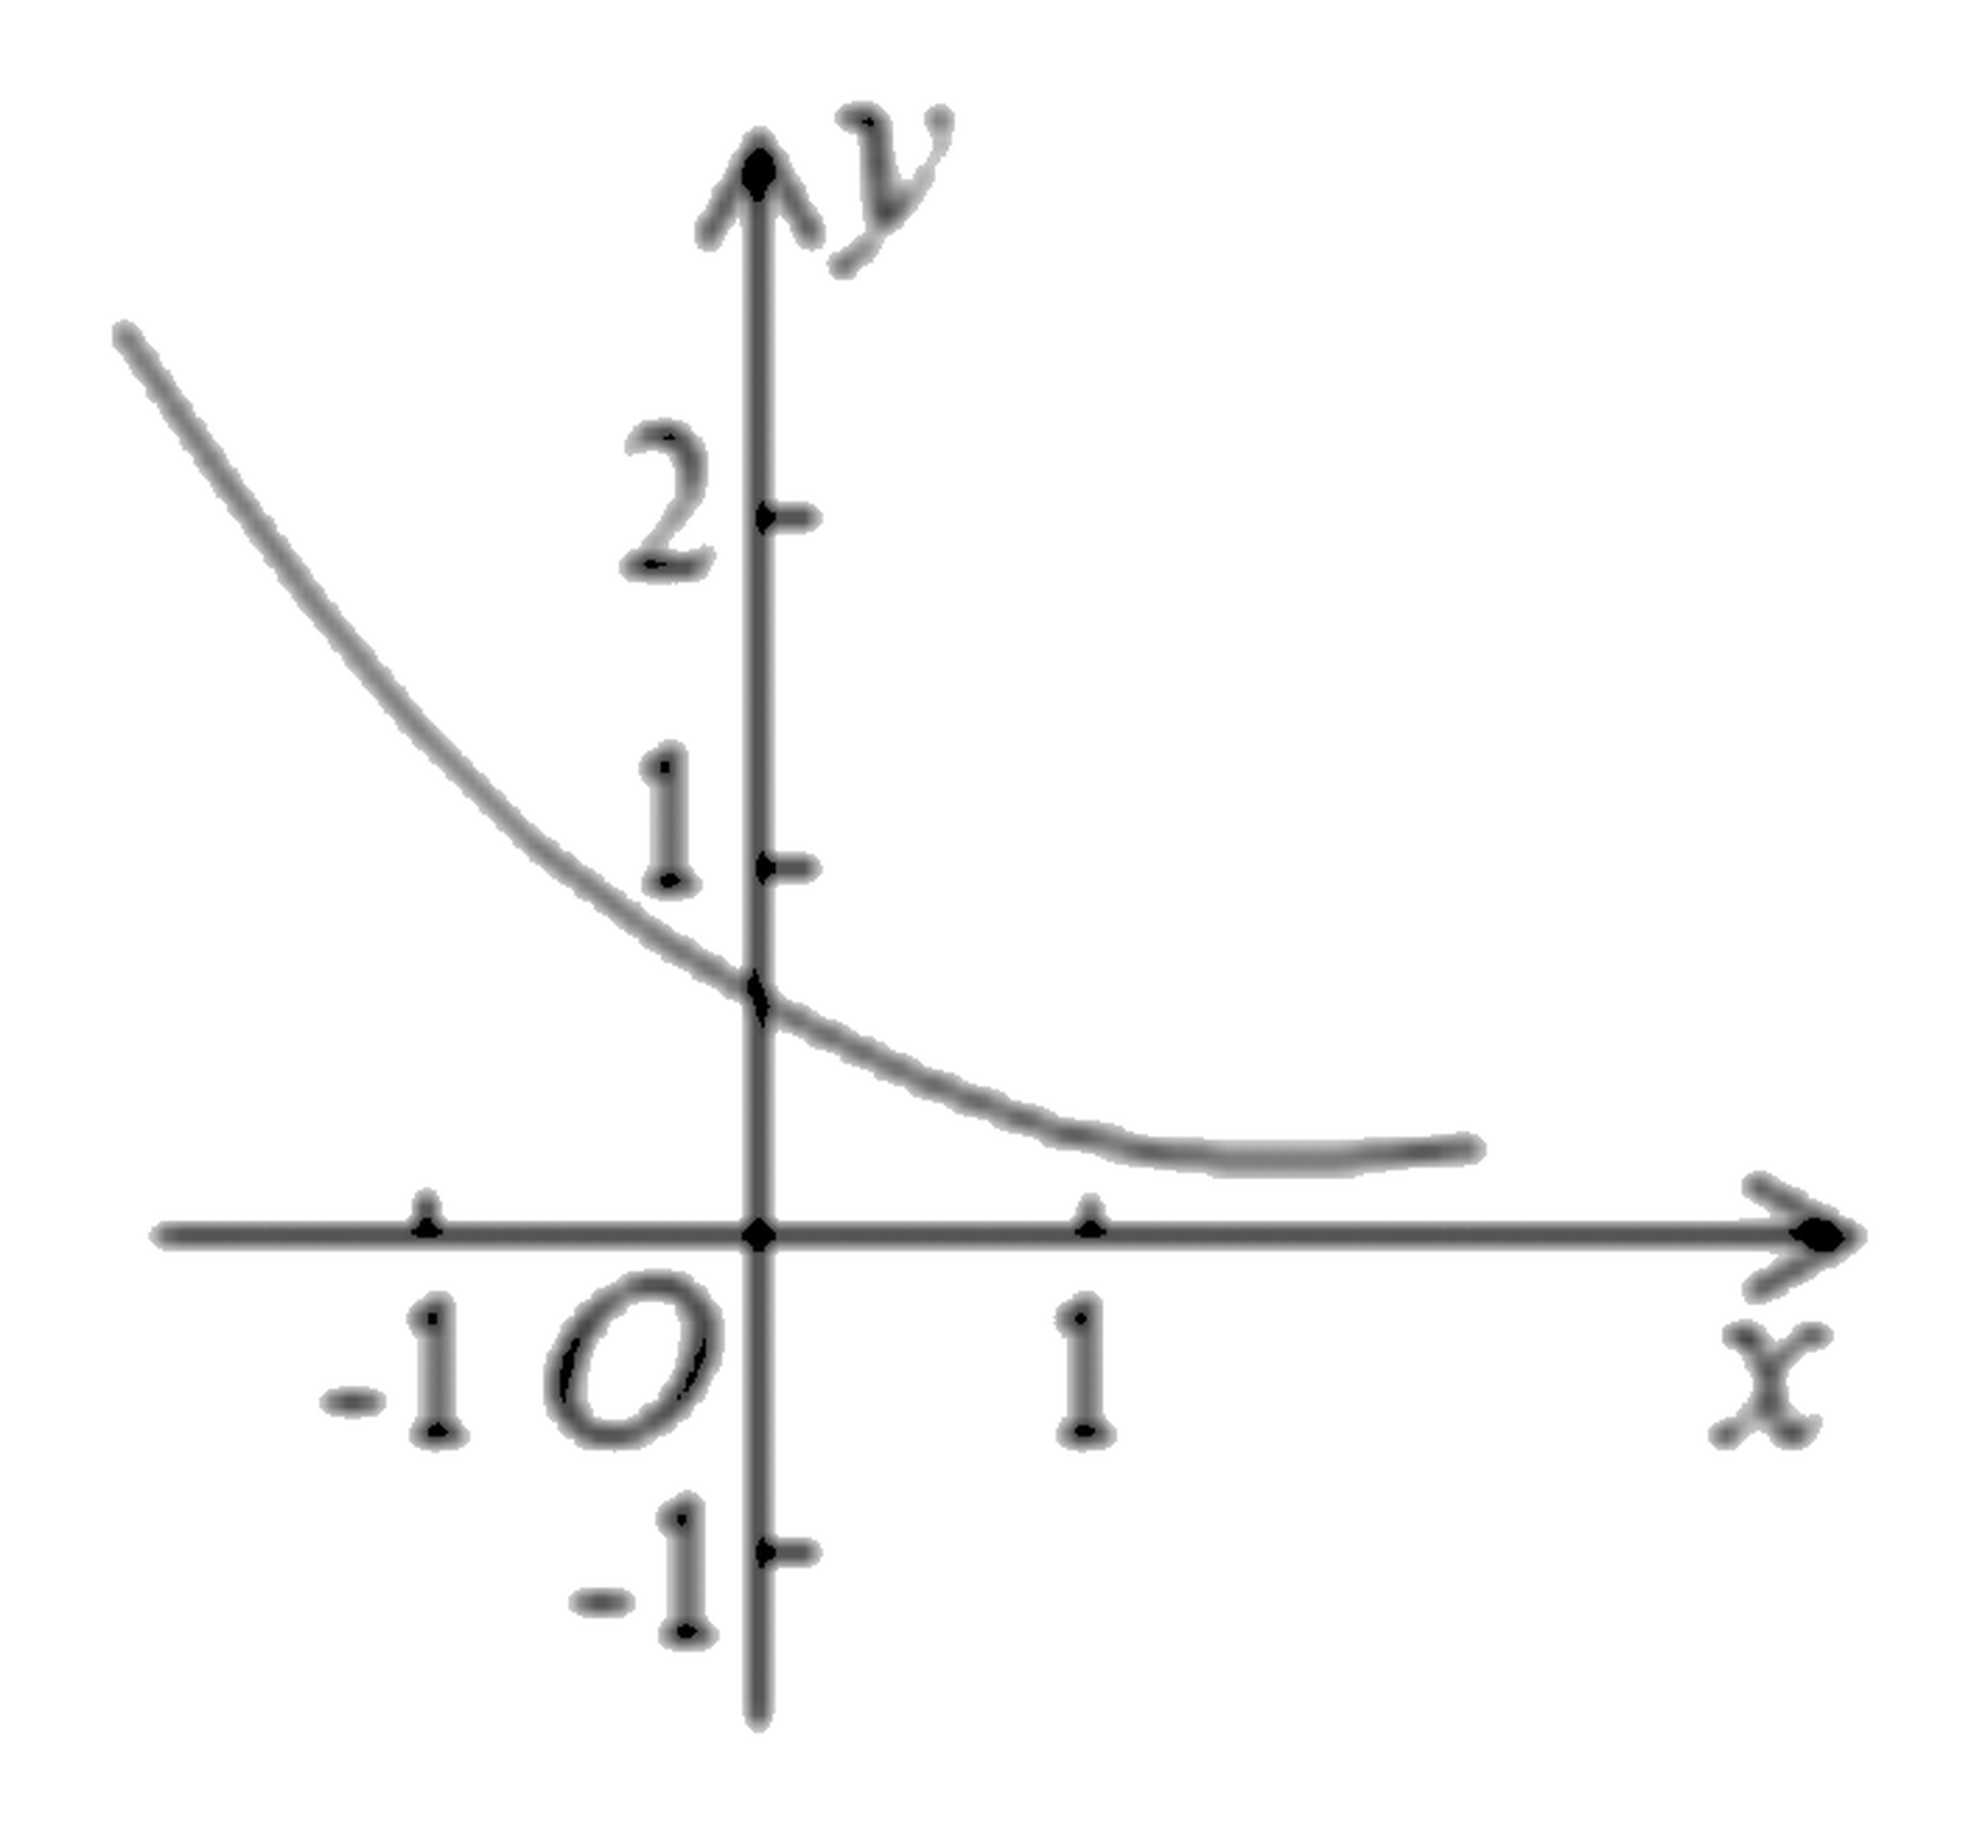
\includegraphics[width=0.30\textwidth]{figures/gao147_q15.png}
\end{center}

\ifanswer
\solbegin
\step{由图象从左到右下降得 $0<a<1$；}
\step{由图象与 $y$ 轴的交点得 $0<a^{-b}<1$，故 $b<0$；}
\step{故 $0<a<1$，$b<0$；故选 $D$.}
\solend
\fi

% === Q16 ===：位数新定义题（无弯引号，放大 04 页 z/q16_stem.png 确认）；四选项横排一行；解析 3 个印刷行
\item 数学运算是指在明晰运算对象的基础上，依据运算法则解决数学问题的素养. 因为运算，数的威力无限；没有运算，数就只是一个符号，对数运算与指数运算是两类重要的运算，对数的运算性质降低了运算的级别，简化了运算，在数学发展史上是伟大的成就. 而位数是指一个自然数有效位的个数，例如：$2^{10}=1024$，所以 $2^{10}$ 的位数为 4. 请你运用所学过的对数运算的知识，估计 $2025^{2026}$ 的位数是\mbox{（\quad）}

\keepwithprev
A. 6697\qquad B. 6698\qquad C. 6699\qquad D. 6700

\ifanswer
\solbegin
\step{设 $2025^{2026}=t$，所以 $\lg t=2026\lg2025$，}
\step{因为 $\lg2025\approx3.3064$，所以 $\lg t\approx6698.8$，}
\step{所以 $t\approx10^{6698.8}\in(10^{6698},10^{6699})$，所以 $2025^{2026}$ 的位数为 6699. 故选 $C$.}
\solend
\fi

\end{enumerate}

\bigsec{三、解答题}

\begin{enumerate}
\setcounter{enumi}{16}

% === Q17 ===：题干＋解析均在 04 页；集合描述竖线 \mid、描述内半角逗号照录；
% 空集 \varnothing、子集 \subseteq（放大 04 页 z/subset_04_q17b.png 确认带下划线）、数集 \R；
% 解析 5 个印刷行，首行末"所以 A=(-∞,-2)∪(3,+∞)"原卷无标点，照录不补
\item 已知集合 $A=\left\{x\mid \dfrac{x+2}{x-3}>0,x\in\R\right\}$，$B=\{x\mid \lvert x-2a\rvert\leqslant2,x\in\R\}$.

(1) 若 $a=1$，求 $A\cap B$；

(2) 若 $A\cap B=\varnothing$，求实数 $a$ 的取值范围.

\ifanswer
\solbegin
\step{由 $\dfrac{x+2}{x-3}>0$，得 $x<-2$ 或 $x>3$，所以 $A=(-\infty,-2)\cup(3,+\infty)$}
\step{(1) 当 $a=1$ 时，$B=\{x\mid \lvert x-2\rvert\leqslant2\}=[0,4]$，于是 $A\cap B=(3,4]$；}
\step{(2) $B=[2a-2,2a+2]$，}
\step{则 $A\cap B=\varnothing\Leftrightarrow[2a-2,2a+2]\subseteq[-2,3]\Leftrightarrow\begin{cases}2a-2\geqslant-2\\2a+2\leqslant3\end{cases}\Leftrightarrow0\leqslant a\leqslant\dfrac{1}{2}$，}
\step{所以实数 $a$ 的取值范围为 $\left[0,\dfrac{1}{2}\right]$.}
\solend
\fi

% === Q18 ===：氟化物／臭氧应用题；"氟化物""（如冰箱等）"全角夹注照录（放大 05 页 z/q18_line1.png 确认）；
% 关系式 $Q=Q_0e^{-0.0025t}$ 原卷独立一行，按一段照录；解析 6 个印刷行
\item 有些家用电器（如冰箱等）使用了氟化物，氟化物的释放破坏了大气上层的臭氧层，使臭氧含量 $Q$ 呈指数函数型变化，在氟化物排放量维持某种水平时，具有关系式

$Q=Q_0e^{-0.0025t}$，其中 $Q_0$ 是臭氧的初始量.

(1) 随时间 $t$ 的增加，臭氧的含量是增加还是减少？

(2) 试估计多少年以后将会有一半的臭氧消失.（用计算器计算）

\ifanswer
\solbegin
\step{(1) 对于函数 $Q=Q_0e^{-0.0025t}$，显然 $Q>0$，}
\step{任取 $t_1$、$t_2\in(0,+\infty)$，且 $t_1<t_2$，则 $t_2-t_1>0$，}
\step{所以 $\dfrac{Q_1}{Q_2}=\dfrac{Q_0e^{-0.0025t_1}}{Q_0e^{-0.0025t_2}}=e^{-0.0025(t_1-t_2)}=e^{0.0025(t_2-t_1)}>e^0=1$，所以 $Q_1>Q_2$，}
\step{故随着时间 $t$ 的增加，臭氧的含量是减少的；}
\step{(2) 令 $\dfrac{Q}{Q_0}=\dfrac{1}{2}$，即 $\dfrac{Q_0e^{-0.0025t}}{Q_0}=e^{-0.0025t}=\dfrac{1}{2}$，得 $-0.0025t=\ln\dfrac{1}{2}\approx-0.6931$，}
\step{解得 $t\approx277$，故估计 277 年以后将会有一半的臭氧消失.}
\solend
\fi

% === Q19 ===：题干用"图像"、解析两处用"图象"逐处照录不统一（05 页）；数集 \Z；
% 题干＋解析前 4 行在 05 页、解析后 3 行在 06 页；解析共 7 个印刷行
\item 已知幂函数 $f(x)=x^{-m^2+4m}(m\in\Z)$ 的图像关于 $y$ 轴对称，且在区间 $(0,+\infty)$ 上是严格增函数.

(1) 求 $m$ 的值；

(2) 求满足不等式 $(2a+1)^m<(a+1)^m$ 的实数 $a$ 的取值范围.

\ifanswer
\solbegin
\step{(1) 由题意得 $-m^2+4m>0$，解得 $0<m<4$，}
\step{因为 $m\in\Z$，所以 $m=1$ 或 $m=2$ 或 $m=3$.}
\step{当 $m=1$ 或 $m=3$ 时，$f(x)=x^3$，图象关于原点对称，不合题意；}
\step{当 $m=2$ 时，$f(x)=x^4$，图象关于 $y$ 轴对称，符合题意，所以 $m=2$.}
\step{(2) 代入 $m=2$，不等式为 $(2a+1)^2<(a+1)^2$，}
\step{得 $(2a+1)^2-(a+1)^2=a(3a+2)<0$，因此 $-\dfrac{2}{3}<a<0$，}
\step{所求范围为 $\left(-\dfrac{2}{3},0\right)$.}
\solend
\fi

% === Q20 ===：指数函数题，题干用"图像"；(3) 长求和式（分数 1/2026、1011/2026、2011/2026、
% 15/2026、1015/2026、2025/2026 放大 06 页 z/q20_sum_06a.png 确认）；题干在 06 页、
% 解析前 6 行在 06 页下半、后 6 行在 07 页上半；解析共 12 个印刷行
\item 已知指数函数 $y=a^x$（$a>0,a\ne1$）的图像经过点 $(1,4)$.

(1) 求实数 $a$ 的值；

(2) 若 $f(x)=(a^x)^2-2\cdot a^x-8$，当 $x\in\R$ 时，不等式 $f(x)>m\cdot4^x-12$ 恒成立，求 $m$ 的取值范围；

(3) 记 $g(x)=\dfrac{1}{a^x+2}$，求证：$g(x)+g(1-x)$ 为定值，并求 $g(0)+g\left(\dfrac{1}{2026}\right)+g\left(\dfrac{1011}{2026}\right)+g\left(\dfrac{2011}{2026}\right)+g\left(\dfrac{1}{2}\right)+g\left(\dfrac{15}{2026}\right)+g\left(\dfrac{1015}{2026}\right)+g\left(\dfrac{2025}{2026}\right)+g(1)$ 的值.

\ifanswer
\solbegin
\step{(1) 将 $(1,4)$ 代入 $y=a^x$，得 $a^1=4$，即 $a=4$.}
\step{(2) 令 $t=4^x$，当 $x\in\R$ 时，$t$ 取遍所有正实数.}
\step{原不等式等价于 $t^2-2t-8>mt-12\Leftrightarrow m<t+\dfrac{4}{t}-2$，}
\step{由基本不等式，$t+\dfrac{4}{t}-2\geqslant2\sqrt{t\cdot\dfrac{4}{t}}-2=2$，}
\step{当且仅当 $t=\dfrac{4}{t}$，即 $t=2$ 时取等号，}
\step{因此原不等式恒成立的充要条件为 $m<2$，即 $m\in(-\infty,2)$.}
\step{(3) 对任意 $x\in\R$，令 $t=4^x>0$，则 $4^{1-x}=\dfrac{4}{t}$，}
\step{从而 $g(x)+g(1-x)=\dfrac{1}{t+2}+\dfrac{1}{\dfrac{4}{t}+2}=\dfrac{1}{t+2}+\dfrac{t}{2(t+2)}=\dfrac{1}{2}$，}
\step{因此 $g(x)+g(1-x)$ 为定值 $\dfrac{1}{2}$.}
\step{原式中，0 与 1、$\dfrac{1}{2026}$ 与 $\dfrac{2025}{2026}$、$\dfrac{1011}{2026}$ 与 $\dfrac{1015}{2026}$、$\dfrac{2011}{2026}$ 与 $\dfrac{15}{2026}$}
\step{分别配对，每对函数值之和均为 $\dfrac{1}{2}$，且 $g\left(\dfrac{1}{2}\right)=\dfrac{1}{4^{\frac12}+2}=\dfrac{1}{4}$，}
\step{所以所求和为 $4\cdot\dfrac{1}{2}+\dfrac{1}{4}=\dfrac{9}{4}$.}
\solend
\fi

% === Q21 ===：不动点新定义题；题干在 07 页、解析续 08／09 页，共 20 个印刷行；
% 判别式两形混用：08 页 (2) cases 内等腰偏高 \Delta、09 页 (3) 扁等边 \triangle，逐处照录不统一
% （放大 /tmp/gao147/z/delta_vs_triangle.png 并排确认）；数集 \R；\forall 照录；
% 第 6—8 行是原卷一个长算式折成的三个印刷行，按印刷行分三条 \step、不并折行
\item 对于二次函数 $y=mx^2+nx+t(m\ne0)$，若存在 $x_0\in\R$，使得 $mx_0^2+nx_0+t=x_0$ 成立，则称 $x_0$ 为二次函数 $y=mx^2+nx+t(m\ne0)$ 的不动点.

(1) 求二次函数 $y=x^2-x-3$ 的不动点；

(2) 若二次函数 $y=2x^2-(3+a)x+a-1$ 有两个不相等的不动点 $x_1$、$x_2$，且 $x_1$、$x_2>0$，求 $\dfrac{x_1}{x_2}+\dfrac{x_2}{x_1}$ 的最小值；

(3) 若对任意实数 $b$，二次函数 $y=ax^2+(b+1)x+(b-1)(a\ne0)$ 恒有不动点，求 $a$ 的取值范围.

\ifanswer
\solbegin
\step{(1) 令 $x^2-x-3=x$，即 $x^2-2x-3=0$，即 $(x-3)(x+1)=0$，}
\step{解得 $x_1=-1$，$x_2=3$，所以不动点为 $-1$ 和 $3$.}
\step{(2) 由题意，$2x^2-(3+a)x+a-1=x$ 有两个不相等的正实数根，}
\step{即方程 $2x^2-(4+a)x+a-1=0$ 有两个不相等的正实数根，}
\step{所以 $\begin{cases}\Delta=(4+a)^2-8(a-1)>0\\x_1+x_2=\dfrac{4+a}{2}>0\\x_1\cdot x_2=\dfrac{a-1}{2}>0\end{cases}$，解得 $a>1$，}% 判别式原卷印等腰偏高粗三角 $\Delta$（放大 08 页 z/delta_08_q21cases.png）
\step{所以 $\dfrac{x_1}{x_2}+\dfrac{x_2}{x_1}=\dfrac{x_1^2+x_2^2}{x_1\cdot x_2}=\dfrac{(x_1+x_2)^2-2x_1\cdot x_2}{x_1\cdot x_2}=\dfrac{(x_1+x_2)^2}{x_1\cdot x_2}-2$}
\step{$=\dfrac{\left(\dfrac{4+a}{2}\right)^2}{\dfrac{a-1}{2}}-2=\dfrac{\dfrac{(a+4)^2}{4}}{\dfrac{a-1}{2}}-2=\dfrac{(a-1+5)^2}{2(a-1)}-2$}
\step{$=\dfrac{(a-1)^2+10(a-1)+25}{2(a-1)}-2=\dfrac{a-1}{2}+\dfrac{25}{2(a-1)}+3$.}
\step{因为 $a>1$，所以 $a-1>0$，}
\step{所以 $\dfrac{a-1}{2}+\dfrac{25}{2(a-1)}+3\geqslant2\sqrt{\dfrac{a-1}{2}\cdot\dfrac{25}{2(a-1)}}+3=8$，}
\step{当且仅当 $\dfrac{a-1}{2}=\dfrac{25}{2(a-1)}$，即 $a=6$ 时等号成立，}
\step{所以 $\dfrac{x_1}{x_2}+\dfrac{x_2}{x_1}$ 的最小值为 $8$.}
\step{(3) 设 $f(x)=ax^2+(b+1)x+b-1$，}
\step{则方程 $f(x)=x$，可化为 $ax^2+(b+1)x+b-1=x$，}
\step{即 $ax^2+bx+b-1=0$，}
\step{由题意得一元二次方程 $ax^2+bx+b-1=0$ 有解，又 $a\ne0$，}
\step{所以方程 $ax^2+bx+b-1=0$ 的判别式 $\triangle=b^2-4a(b-1)\geqslant0$，}% 判别式原卷印扁等边细线三角 $\triangle$（放大 09 页 z/triangle_09_q21.png），与 (2) 高 $\Delta$ 混用、照录不统一
\step{即 $b^2-4ab+4a\geqslant0$，则该不等式对 $\forall b\in\R$ 恒成立，}
\step{则 $(4a)^2-4\times4a\leqslant0$，且 $a\ne0$，解得 $0<a\leqslant1$，}
\step{所以实数 $a$ 的取值范围是 $(0,1]$.}
\solend
\fi

\end{enumerate}

\end{document}
